% =========================================
% == Latex-Template for Theses
% == by René Schönfelder
% == schoenfr@isp.uni-luebeck.de
% =========================================
% 
% This latex project serves as a template for theses in the MINT section of the
% University of Lübeck. The first version was created during the authors
% master's and steadily evolved from there on.
% 
% The template may be used and distributed freely. In the case of questions or
% suggestions just send an email to schoenfr@isp.uni-luebeck.de. This document
% is in english so that international students may also profit from this
% template. However, the content is written in german because the guidelines
% expect german theses and most students are writing in german..

% The document class ``scrbook'' describes books:
\documentclass[
  a4paper,               % a4 paper
  twoside,               % two-sided
  headings=small,        % make headings smaller
  DIV=12,                % divide the paper in 12 parts
  BCOR=8mm,              % 8mm binding correction
  headinclude=true,      % use a header
  footinclude=false,     % do not use a footer
  numbers=noenddot,      % no dot after last number in headings
  11pt]{scrbook}         % font size 11pt

% Encodings
\usepackage[T1]{fontenc}
% Use this for UTF8 input in .tex-files
\usepackage[utf8]{inputenc}
% You can use english alternatively
\usepackage[ngerman]{babel}

% PDF properties
\usepackage{hyperref}
\hypersetup{
  pdfauthor={Moritz Krebbel},
  pdfsubject={Drive-by cache attacks},
  pdftitle={Ausnutzung spekulativer Ausführung durch drive-by Cache-Angriffe},
  pdfkeywords={chache attacks, drive-by attacks, speculative execution}
}

% Color for Corporate Design
\usepackage{xcolor}
\definecolor{oceangreen}{cmyk}{1,.0,.20,.78}

% If you want to color the headings, then you can use the following command. It
% makes most of your pages colored. Please notice, that printing colored pages
% may be a lot more expensive than printing gray scale.
%\addtokomafont{sectioning}{\rmfamily\color{oceangreen}}

% We use the font family ``Palatino'', which does not correspond to the
% guidelines but is still valid. You could also use \usepackage{times}.
\usepackage{palatino}
\fontfamily{ppl}
\selectfont

% General packages
\usepackage{blindtext}
\usepackage{graphicx}               % Include graphics
\usepackage{appendix}               % Use an appendix
\usepackage{textpos}                % Easy text positioning
\usepackage{typearea}               % Standard for defining geometry
\usepackage{tikz}                   % TikZ pictures
\usepackage{amsmath,amssymb,amsthm} % Math
\usepackage{scrhack}
\usepackage{listings}               % Listings
\usepackage[ruled,vlined,linesnumbered]{algorithm2e} % Algorithms
\usepackage{stmaryrd}               % Lightning arrow \lightning
\usepackage{url}                    % Formatting URLs
\usepackage{rotating}               % Rotation of figures
\usepackage{todonotes}              % Make TODO-notes
% This package is used for the following spacing options
\usepackage{setspace}
\usepackage[linguistics]{forest}
\usepackage{breqn}
\usepackage{color}
\usepackage{environ}
\usepackage{minted}

%set size of algorithm env
\SetAlFnt{\small}

\makeatletter
\newsavebox{\measure@tikzpicture}
\NewEnviron{scaletikzpicturetowidth}[1]{%
  \def\tikz@width{#1}%
  \def\tikzscale{1}\begin{lrbox}{\measure@tikzpicture}%
  \BODY
  \end{lrbox}%
  \pgfmathparse{#1/\wd\measure@tikzpicture}%
  \edef\tikzscale{\pgfmathresult}%
  \BODY
}
\makeatother

\usepackage{chngcntr}               % Do not reset the counter for footnotes
\counterwithout{footnote}{chapter}  % on every new chapter

\usepackage{eurosym}
\usepackage{newunicodechar}
\newunicodechar{€}{\euro}

\usepackage{textcomp}

\renewcommand{\algorithmcfname}{Algorithmus}

\newcommand{\twodots}{\mathrel{{.}\,{.}}\nobreak}

% Listing style
\lstset{
  basicstyle={\ttfamily \footnotesize},
  language = Java,
  numbers=left, numberstyle=\tiny,
  frame=tb, framerule=1pt,
  xleftmargin=0.2cm, linewidth=1\textwidth,
  %backgroundcolor=\color{bg},
  keywordstyle=\bf\color{oceangreen},
  morecomment=[l][\color{blue}]{\/*, \*/},
  %emph={for,end,while,function,if,else},
  emphstyle={\color{blue}}
}

\definecolor{lightgray}{rgb}{.9,.9,.9}
\definecolor{darkgray}{rgb}{.4,.4,.4}
\definecolor{purple}{rgb}{0.65, 0.12, 0.82}

\lstdefinelanguage{JavaScript}{
  keywords={typeof, new, true, false, catch, function, return, null, catch, switch, var, if, in, while, do, else, case, break},
  keywordstyle=\color{blue}\bfseries,
  ndkeywords={class, export, boolean, throw, implements, import, this},
  ndkeywordstyle=\color{darkgray}\bfseries,
  identifierstyle=\color{black},
  sensitive=false,
  comment=[l]{//},
  morecomment=[s]{/*}{*/},
  commentstyle=\color{purple}\ttfamily,
  stringstyle=\color{red}\ttfamily,
  morestring=[b]',
  morestring=[b]"
}

\lstset{
   language=JavaScript,
   extendedchars=true,
   basicstyle=\footnotesize\ttfamily,
   showstringspaces=false,
   showspaces=false,
   numbers=left,
   numberstyle=\footnotesize,
   numbersep=9pt,
   tabsize=2,
   breaklines=true,
   showtabs=false,
   captionpos=b
}

\newif\ifonline
\IfFileExists{nored.tex}{\onlinefalse}{\onlinetrue}

\newcommand{\newtext}{\ifonline\color{red}\fi}
\newcommand{\newtextend}{\ifonline\color{black}\fi}

% If you want to list your bib as a usual section listed in the table of
% contents, you can use the following commands.
%\makeatletter
%\renewcommand*\bib@heading{%
%  \chapter{\refname}
%  \@mkboth{\refname}{\refname}
%}
%\makeatother

% Prevent warnings ``hbox badness'' in the bibliography
\usepackage{etoolbox}
\apptocmd{\sloppy}{\hbadness 10000\relax}{}{}

% Prevent a lot of ``hbox badness'' warnings
\setlength{\emergencystretch}{1em}

% 1.5 line spacing (the guidelines say at most 1.2, but we decided to allow
% up to 1.5)
\setstretch{1.5}

% No indentation in the beginning of a paragraph
\setlength{\parindent}{0pt}

% The space between two paragraphs
%\setlength{\parskip}{1em}

% More space inside of tables
% \renewcommand*\arraystretch{1.5}

% Do not number subsubsections
\setcounter{secnumdepth}{2}
\setcounter{tocdepth}{2}

% Load macros and hyphenations
% This file contains various useful definitions
% You may also add your own macros here

% Theorem environments
\newtheorem{definition}{Definition}[chapter]
\newtheorem{proposition}[definition]{Proposition}
\newtheorem{theorem}[definition]{Theorem}
\newtheorem{corollary}[definition]{Corollary}
\newtheorem{conjecture}[definition]{Conjecture}
\newtheorem{lemma}[definition]{Lemma}
\renewenvironment{proof}{\textbf{Proof.}}{%
  \nopagebreak{\par\hfill\textbf{\qed}}\par%
}

% Math structures
\newcommand{\with}{{\ |\ }}
\newcommand{\set}[1]{\left\{#1\right\}}
\newcommand{\abs}[1]{\left|#1\right|}
\newcommand{\norm}[1]{\left\|#1\right\|}
\newcommand{\floor}[1]{\left\lfloor#1\right\rfloor}
\newcommand{\ceil}[1]{\left\lceil#1\right\rceil}
\newcommand{\id}[1]{\text{#1}}
\newcommand{\isdef}{:=}
\DeclareMathOperator*{\argmax}{arg\,max}
\DeclareMathOperator*{\argmin}{arg\,min}

% Math symbols
\newcommand{\E}{\mathbb E} % Expected value
\newcommand{\N}{\mathbb N} % Natural numbers
\newcommand{\Z}{\mathbb Z} % Integer numbers
\newcommand{\R}{\mathbb R} % Real numbers
\newcommand{\C}{\mathbb C} % Complex numbers
\newcommand{\Q}{\mathbb Q} % Rational numbers
\newcommand{\B}{\mathbb B} % Boolean values

\newcommand{\X}{\textbf{X\ }}
\newcommand{\U}{\textbf{\ U\ }}
\newcommand{\F}{\textbf{F\ }}
\newcommand{\G}{\textbf{G\ }}
\newcommand{\true}{\textbf{true}}
\newcommand{\false}{\textbf{false}}
% You can define hyphenations as follows

\hyphenation{Trans-for-ma-tion}


% The actual document starts here
\begin{document}
  % The pages in the front are numbered with roman numerals.
  \frontmatter
  % There are specific guidelines on how to write the title page. This is an
% example of how it could look like. Please notice, that even if your thesis is
% written in english, the title page has to be in german. If you don't speak
% german, ask your advisor for help.
\begin{titlepage}

% Use single-spaced line breaking just for the title page
{\setstretch{1.0}

% Additional top margin
\vspace*{1cm}

% Logo of the institute

\includegraphics[height=2.5cm]{pictures/its-logo.png}
%\includegraphics[height=2.5cm]{pictures/isp_de.png}
% If you are interested in other logos, ask your advisor

% Margin between logo and title
\vspace*{2.5cm}

% YOU HAVE TO WRITE YOUR TITLE IN BOTH LANGUAGES! German and english!

%Drive-By Cache Angriffe auf die RSA Schlüsselgenerierung ODER
%Cache Angriffe auf die RSA Schlüsselgenerierung im Browser ODER
%Browserbasierte Cache Angriffe auf die RSA Schlüsselgenerierung


% The german title of your thesis
\textbf{\LARGE{Browser-basierte Cache-Angriffe auf die\\RSA-Schlüsselgenerierung}} \vspace*{1em} \\
% The english title of your thesis
\textit{\LARGE{Browser-based Cache Attacks on RSA key generation}}

% 2 lines of space
\vspace*{2em}

% Type of this thesis
\textbf{Masterarbeit}

% Spacing
\vspace*{1em}

% Your course of study
im Rahmen des Studiengangs \\ % within the study courses of
\textbf{Informatik} \\ % computer science or informatics (both are ok)
der Universität zu Lübeck % at the University of Lübeck

% Spacing
\vspace*{1.5em}

% Your name
vorgelegt von \\ % handed in by
\textbf{Moritz Krebbel}

% Spacing
\vspace*{1.5em}

% Name of your supervisor
ausgegeben und betreut von \\ % issued and supervised by
\textbf{Prof.\ Dr.\ Thomas Eisenbarth}

% Spacing
\vspace*{1.5em}

% Optional information about scientific assistance
mit Unterstützung von \\ % with the assistance of
Ida Bruhns

% Spacing
\vspace*{2em}

\vfill

% TODO: Remember to put the correct date here
Lübeck, den \today
}
\end{titlepage}

  %\chapter*{Abstract}
\todo{Der zweite Titel gefällt mir besser, was meinst du?}
%Einleitungssatz (zu thema hinführen): 
\todo{ja, du brauchst einen Einleitungssatz, aber ohne Meltdown/Spectre. Irgendwas in Richtung: Mikroarchitekturangriffe haben sich als sehr mächtig erwiesen, erfordern aber meist ausführung von code auf der Opfermaschine. Allerdings wurde durch PAPER gezeigt, dass auch aus Browser möglich. Solche Angriffe werden in Skriptsprachen usw. und sind besonders verherend, weil... . }
%Eventuell Meltdown und Spectre als Aufhänger nutzen
Browser-basierte Seitenkanalangriffe auf die Mikroarchitektur der CPU sind besonders verehrend, da bereits der Besuche einer Webseite ausreicht, um Opfer eines Angriffs zu werden.

%kurz näher beschreiben wie das in etwa funktionert:
So ein Angriff wird in Scriptsprachen wie Javascript implementiert und nutzt den geteilten L3-Caches der CPU aus, um Informationen über die Speicherzugriffe anderer Programme zu erhalten.
Der Angriff ist weder auf einen Exploit im Browser noch auf fahrlässiges Verhalten der Nutzer angewiesen.


%was passiert in dieser Arbeit/Was sind wesentlich Ergenisse?
%-Neue potenzielle gefährliche leakage in NSS und OpenPGP.js
%-versuchte Portierung eines nativen RSA-Schlüsselgenerierungsangriff auf OpenSSL zu browsbasierten Angriff auf NSS
%-Probleme bei Portierung wie Bremsen, verminderte Angriffsgeschwindigkeit im Browser werden analysiert
%-Eviction-Set-Suchalgorithmus wird verbessert, neue Variante beschrieben und mit altem Algorithmus verglichen

In dieser Arbeit \todo{wurde der Drive by angriff nachimplementiert und es wurde versucht, den nativen Angriff auf RSA-Primzahlgenerierung (QUELLE) in den Browser zu portieren. Zusätzlich wurden} werden neue Leakages in der RSA-Primzahlgenerierung von Mozilla NSS und OpenPGP.js analysiert und Nachteile die gegenüber einem nativen Angriff bestehen, erörtert.
Exemplarisch wird die Portierung eines nativ laufenden Angriffs auf die RSA-Primzahlgenerierung zu einem Browserangriff 
untersucht und auftretende Fallstricke\todo{besser: Schwierigkeiten} beschrieben.
Des Weiteren wird ein neuer \todo{Algorithmus zum finden von eviction sets} Eviction-Set-Algorithmus vorgestellt, der die in der Praxis wichtige Initalisierungsphase eines L3-Cache-Angriffs beschleunigt. 
  %% This declaration is essential to every thesis. You need to declare, that this
% work is done by yourself. It is necessary to write ``an Eides statt''.

\chapter*{Erklärung}
Ich versichere an Eides statt, die vorliegende Arbeit selbstständig und nur
unter Benutzung der angegebenen Hilfsmittel angefertigt zu haben.

\vspace{5em}

% You need to personally sign your thesis here. DO NOT FORGET THIS!!!

\rule{0.4\textwidth}{0.4pt}

Lübeck, \today

  %\chapter*{Acknowledgements}

% Replace this blind text with your acknowledgements
\blindtext

  \tableofcontents

  % In the main matter the pages are numbered with arabic numerals.
  \mainmatter
  %\chapter{Einführung}
\label{chapter:introduction}

%(Es fehlt mir ein einleitender Satz wie etwa "Im Bereich der IT-Sicherheit gewinnt der externe Zugriff auf Daten anderer (wer sind diese anderen genau?) zunehmende Bedeutung (gute Einleitung, aber warum und für wen sind diese Angriffe interessant?).") 
Seitenkanalangriffe sind ein mächtiger Angriff, da sie es unter anderem erlauben, geheime Informationen wie den kryptografischen Schlüssel aus einem Gerät wie einer Chipkarte zu extrahieren.
Hierfür wird beispielsweise der Stromverbrauch oder die Berechnungsdauer verschiedener Ein- und Ausgaben gemessen.
Bei solchen physikalischen Seitenkanalangriffen ist die Angreiferin gezwungen, eine örtliche Nähe zum System zu besitzen.

Seitenkanalangriffe auf die Mikroarchitektur eines Prozessors sind von dieser Einschränkung befreit, da die
Ausführung von Programmcode %einem /dem  (welchem? oder gibt es nur einen?) allgemein gemeint
auf dem Zielsystem ausreicht.
Seit der ersten Beschreibung von Seitenkanalangriffen auf die Mikroarchitektur vor über zehn Jahren \cite{FirstCacheAttackDES} sind diese zu einem ernst zu nehmenden Sicherheitsrisiko herangewachsen \cite{OpenBSDHyperthreading}.

Auf der Mikroarchitekturebene konkurriert der Opferprozess mit dem Angriffsprozess um die Ressourcen des Prozessors, selbst wenn der Angriffsprozess mit keinen außerordentlichen Privilegien ausgestattet ist.
Aufgrund dieser Konkurrenz kann die Angreiferin %(erneut weiblich? generneutrale Formulierung: der Angreifende oder die angreifende Person)
Informationen über den Opferprozess gewinnen, indem sie durch Messungen Varianzen beim Zugriff auf die Ressourcen feststellt.

Eine Reihe von Ressourcen hat sich durch das Leaken von Informationen als problematisch erwiesen, etwa die Einheiten der Sprungvorhersage oder der Return-Stack-Buffer.
Das mit Abstand größte Problem stellen die vielfältigen Caches dar, welche eine Überwachung der Speicherzugriffe des Opferprozesses erlauben.
Diese ermöglichen es, geheime Informationen wie kryptografische Schlüssel von RSA \cite{CacheBleedOpenSSLRSA} oder AES \cite{BernsteinAES} aus dem Opferprozess zu extrahieren.
Weitere Anwendungsmöglichkeiten sind Keylogger \cite{Keylogger} und Überwachungen der Webseitenaufrufe oder Nutzeraktivitäten \cite{TheSpyInTheSandbox}.

Es ist trotz dieser Möglichkeiten wenig darüber bekannt, ob Cache-Angriffe praktisch relevant sind oder wie häufig sie eingesetzt werden.
Einem breiten Angriffsvektor steht das im Großteil der Literatur angenommene Angriffsszenario entgegen, welches die Ausführung von nativem Code auf dem Opfersystem voraussetzt.
Dieses Szenario hat seine Berechtigung unter anderem bei Angriffen auf virtuelle Maschinen, wo der Code der Angreiferin auf derselben Hardware wie der des Opferprozesses läuft (Cross-VM-Attack).

Auch Mehrbenutzersysteme, wie sie häufig in Unternehmen und Organisationen anzutreffen sind, fallen unter dieses Szenario.
So ist es jedem Studierenden der Universität zu Lübeck jederzeit möglich, sich per SSH auf einen beliebigen Pool-Rechner einzuloggen, unabhängig davon, ob der Rechner lokal in Benutzung ist.

In einem typischen Endbenutzerszenario ist es realitätsfern vorauszusetzen, dass vom Opfer nativer Angriffscode ausgeführt wird.
Denn den meisten Benutzern ist die einhergehende Gefahr der Ausführung von unbekanntem nativem Code bewusst, und zudem würden mögliche Cache-Angriffe das geringste Problem darstellen. (Warum?)

Daher gibt es Bestrebungen, Cache-Angriffe auf Endbenutzergeräte zu ermöglichen \cite{TheSpyInTheSandbox,DriveByPaper,ASLROnTheLine}, indem der Angriffscode in Websprachen wie Javascript übersetzt und vom Browser des Opfers ausgeführt wird.
Da der Browser faktisch bei jedem Webseitenbesuch fremden und unbekannten Code ausführt, jedoch auch keine Angriffsfläche bieten soll, sind Möglichkeiten für die Angreiferin (weiblich?) in Javascript und Co. entsprechend restriktiv.
Auf Grund dieser Tatsachen sind Angriffe im Browser nur eingeschränkt oder aufwendiger auszuführen, wie sich im Verlaufe dieser Arbeit zeigen wird. 

\section{Aufgabenstellung}

%\todo{Ich wäre hier für section Aufgabenstellung. Außerdem ein kleines bisschen blabla: In Dieser Arbeit wird der Angriff aus PAPER nachimplementiert. Es handelt sich dabei um einen P and P Angriff, der über TECHNOLOGIE durchgeführt wird. Durch TECHNOLOGIE bekommt man VORTEILE. Im Laufe der Implementierung werden folgende Fragen bearbeitet: }

In dieser Arbeit wird unter anderem der Angriff aus dem Paper \cite{RSAKeyGeneration2} auf Mozilla NSS portiert. Es handelt sich dabei um einen Prime-and-Probe-Angriff, der im Gegensatz zum Original-Paper über Javascript bzw. Webassembly durchgeführt wird. Dadurch erhöht sich die Zahl potenzieller Opfer, da der Angriff über eine Webseite oder Werbung auf dieser ausgerollt werden kann.
Außerdem werden neue Leakages in der RSA-Primzahlgenerierung von Mozilla NSS und OpenPGP.js analysiert und ihre Einsatzmöglichkeiten bei einem praktischen Angriff überprüft.

%\todo{Ist das genug?}

Im Laufe der Arbeit werden folgende Fragen beantwortet:

\begin{enumerate}
\item Unter welchen Bedingungen sind im Oktober 2018 Cache-Angriffe aus dem Browser heraus möglich?
Die Arbeiten \cite{TheSpyInTheSandbox,DriveByPaper,ASLROnTheLine} haben demonstriert, dass Cache-Angriffe im Browser möglich sind.
Allerdings sind diese vor den Gegenmaßnahmen der Browserhersteller gegen Meltdown und Spectre veröffentlicht worden.

\item Welchen Einschränkungen unterliegen die Cache-Angriffe im Browser gegenüber Cache-Angriffen mit nativem Code?

\item Wie kann die Initialisierung des Angriffs, das heißt die notwendige Eviciton-Set-Suche beschleunigt werden?

\item Gibt es im Bereich der RSA-Schlüsselgenerierung Leakages, die Informationen über den Schlüssel verraten und sind diese im Browser ausnutzbar?
\end{enumerate}

%\section{Ergebnisse}
%\todo{diese Section (unterteilung, nicht Inhalt) kann dafür meinetwegen weg}

Für die Beantwortung der ersten Frage spielt der Browser eine wichtige Rolle, da für Cache-Angriffe hochauflösende Timer im Nanosekundenbereich benötigt werden.
In Chrome ist das Erzeugen eines solchen Timers durch einen Counter-Thread standardmäßig möglich, wobei dies in Firefox zurzeit ausschließlich durch Veränderung der Browsereinstellungen möglich ist.
Der angesprochene Counter-Thread ist während des gesamten Angriffs voll ausgelastet, belegt also einen ganzen virtuellen Kern.
Da Entwickler hochauflösende Timer nachfragen, wird Mozilla ebenso wie Google in Zukunft versuchen, wieder hochauflösende Timer anzubieten, wobei der zurzeit nötige Timer-Thread entfallen wird.
Dies wird passieren, sobald Maßnahmen gegen Meltdown und Spectre implementiert sind (siehe Abschnitt \ref{GooglePageIsolation}).

\par \medskip  

%\todo{das hier finde ich albern. Du kannst dir gern den Absatz umdefinieren, sodass du bei jedem Absatz einen medskip hast. Aber hier plötzlich damit anfangen finde ich komisch.}
%\todo{Sollte nur hier als Stilmittel verwendet werden, damit die Absätze den obigen Fragen besser zugeordnet werden können.}

Beim Prime-and-Probe-Angriff steht die Browserimplementation einer nativen Implementation in nichts nach. Allerdings ist neben den Kosten für den Counter-Thread die zeitliche Auflösung des Angriffs um \todo{c code slot time messen} TODO \% reduziert.

Der Opferprozess wird oft künstlich gebremst, da die Berechnungen auch beim Angriff mit nativem Code häufig zu schnell sind.
Auch im Browser lassen sich Methoden umsetzen, um den Opferprozess zu bremsen. %\todo{bremsvergleich c vs wasm/js}
Aufgrund der fehlenden clflush-Instruktion, ist die damit verwendete Bremsmethode im Browser nicht umsetzbar.
Anhand eines Angriffs auf die RSA-Schlüsselgenerierung wird gezeigt, dass die Portierung eines nativ laufenden Angriffs aufgrund dieser Einschränkungen nicht immer möglich ist.

\par \medskip  

Um einen realistischen Angriff zu erhalten, ist eine kurze Initialisierungsphase Voraussetzung.
Der in vielen Papers beschriebene Eviction-Set-Suchalgorithmus \cite{PrimeAndAbort, LiuPrimeAndProbe, DriveByPaper} wurde in vielerlei Hinsicht optimiert und die Ergebnisse anschließend mit der ursprünglichen Variante verglichen. 
Des Weiteren wurde eine neue noch unveröffentlichte Technik im Kontext der Eviction-Set-Suche im Browser erprobt.
Diese nutzt spezifische Eigenschaften der Store-Queue in Intel-Prozessoren aus.
Damit kann die Suche gegenüber dem optimierten Standardalgorithmus um etwa den Faktor 4 beschleunigt werden.

%Wenn mehr als eine Cache-Line überwacht werden soll, ist es für die zeitliche Auflösung von Vorteil, mehrere Angriffsinstanzen zu starten.
%Diese müssen jedoch die Eviction-Set-Suche nacheinander durchführen, da sie sich ansonsten gegenseitig beeinflussen würden.
%Somit würde sich der Performancevorteil in diesen Fällen amplifizieren (besser: erhöhen).

\par \medskip  

Es wurden sowohl die Schlüsselgenerierung von Mozilla NSS als auch von OpenPGP.js auf Leakages untersucht. 
%Zum Einsatz kam dabei ein Werkzeug (Welches ist das? Wie heißt es?), welches automatisch potenzielle Leakages aufdeckt.
Sowohl in der Primzahlgenerierung von Mozilla NSS als auch OpenPGP.js wurden Leakages entdeckt, welche die verwendeten Primzahlen in einem Gleichungssystem beschreiben.
Es konnte noch nicht abschließend geklärt werden, ob diese Gleichungssysteme bei praktischen Instanzen wie RSA-2048 in annehmbarer Zeit gelöst werden können.

Des Weiteren wurde ein bekannter Cache-Angriff auf die RSA-Schlüsselgenerierung in OpenSSL nach Mozilla NSS portiert.
Der ursprüngliche Angriff setzte die Ausführung nativen Codes voraus, wobei in dieser Arbeit eine Umsetzung im Browser geprüft wurde.
Dabei konnten mehrere Probleme identifiziert werden, welche Portierungen von nativen Cache-Angriffen hin zu Implementierungen im Browser erschweren. 
Diese werden in Kapitel \ref{chapter:results} und \ref{chapter:discussion} genauer beschrieben und beurteilt.

\section{Forschungsstand/Verwandte Arbeiten}
\label{related_work}

Hier soll ein Überblick bereits getätigter Forschungsarbeiten im Rahmen der für die Arbeit relevanten Themenbereiche Drive-by-Attacks und Angriffe auf die RSA Schlüsselgenerierung gegeben werden. Zudem soll eine Abgrenzung gegenüber verwandten, aber für diese Arbeit nicht relevanten Themenbereichen stattfinden.

%\subsection{Cache-Angriffe}

%Cache-Angriffe sind kein neues Phänomen \cite{BernsteinAES, CacheAttacksCountermeasuresAESShamir}, sondern wurden schon im Jahr 2003 \cite{DESCacheAttack2003} erstmals beschrieben.
%Die ersten Angriffe zielten auf den L1- und L2-Datencache \cite{CacheAttacksCountermeasuresAESShamir} ab, wobei die Angriffe mit der Zeit auf andere Caches, wie den L1-Instruktionscache \cite{NewResultsInstructionCacheAttacks} und den geteilten L3-Cache \cite{CacheAttacksCloud, LiuPrimeAndProbe} ausgeweitet wurden.
%Des Weiteren wurden mit dem Return-Stack-Buffer \cite{Maisuradze2018ret2specSE} und der Sprungvorhersage \cite{BranchPredictionVulnerabilitiesOpenSSL, PredictingSecretKeysViaBranchPrediction, CovertChannelsThroughBranchPredictors} auch andere Cache-Typen angegriffen.
%Einen guten Überblick bietet das Survey-Paper von Qian ge et al. \cite{SurveyTimingAttacksCountermeasures}, wobei dies Ende 2016 veröffentlichte Paper aktuelle Entwicklungen nicht berücksichtigen kann.

\subsection{Cache-Angriffe im Browser}

Alle oben zitierten Arbeiten setzen die Ausführung von nativem Code auf dem Opfersystem voraus. Im Jahr 2015 wurde die erste Arbeit \cite{TheSpyInTheSandbox}, welche sich mit Cache-Angriffen im Browser beschäftigt, veröffentlicht.
Die Autoren konnten den Aufruf von verschiedenen bekannten Webseiten unterschiedlichen Cache-Zugriffsmustern zuordnen, um so das Surfverhalten von Nutzern zu überwachen.
Gras et al. \cite{ASLROnTheLine} konnten im Browser erfolgreich die Speicherverwürfelung ASLR aushebeln, wobei sich der Angriff aufgrund der niedrigen zeitlichen Auflösung nicht zur Schlüsselextraktion eignet.

Mit dem Rowhammer-Angriff \cite{Rowhammer} ist es möglich, Bits im Speicher ohne Schreibzugriffe zu verändern, um beispielsweise Sicherheitsvorkehrungen zu umgehen. 
Dieser wurde von Gruss et al. erfolgreich in Javascript implementiert \cite{RowhammerJS}.

Code, der im Hinblick darauf designt wurde, unabhängig von den Eingaben dieselbe Laufzeit und denselben Codepfad zu besitzen, verhindert viele Leakages.
Im Paper \cite{DriveByPaper} wurde dargestellt, dass solcher Code durch die Ausführung im Browser angreifbar werden kann.
Durch die Freiheiten des Javascript-Compilers ist es möglich, je nach Eingabe unterschiedliche Codepfade auszuführen und somit eine Leakage entstehen zu lassen.

\subsection{Cache-Angriffe auf RSA}

Viele Paper haben gezeigt \cite{CacheBleedOpenSSLRSA, FlushReload, DriveByPaper}, dass sich der RSA-Schlüssel oder Teile davon mittels Cache-Angriffen extrahieren lassen. Das Angriffsziel waren dabei Komponenten der Ver- und Entschlüsselung, beispielsweise die modulare Exponentiationsfunktion \cite{CacheBleedOpenSSLRSA, DriveByPaper, DriveByPaper}. 

%\todo{Hier vielleicht noch ein bisschen mehr darüber, wie diese Angriffe ablaufen? Traces von Multiplier-Tabellen sammeln, dann auswerten? Muss auch nicht, wäre nur Masse}

Weniger Aufmerksamkeit wurde der RSA-Schlüsselgenerierung geschenkt, da diese im Gegensatz zur Ver- und Entschlüsselung nur einmal ausgeführt wird und damit schwieriger anzugreifen ist.
In der 2018 verfassten Arbeit \cite{RSAKeyGeneration2} wird ein Angriff auf die RSA-Schlüsselgenerierung in OpenSSL beschrieben.
Hierfür wird die Funktion zum Finden des größten gemeinsamen Teilers angegriffen, welche die Teilerfremdheit der beiden erzeugten Primzahlen $p$ und $q$ zu dem Exponenten $e$ überprüft.

%\todo{Trotzdem gibt es hier ein Paper. Dies ist die Stelle, an der du es beschreiben solltest. Dieses Paper bildet jetzt etwa 30 Prozent der Grundlage dieser Arbeit, da sollte mehr zu stehen. }

%\cite{BSIRSAKeyGeneration}  

% \subsection{Spekulative Ausführung, Enklaven und Hyperthreading}
% \label{relatedWorkHyperthreading}

% %\todo{hier fehlt völlig der BEzug zu deiner Arbeit. Du müsstest hier noch schreiben, dass wir diese Lücken nicht ausnutzen und dir einen Grund ausdenken warum wir das nicht tun. }
% %Verweis auf Diskussion von Meltdown und Spectre im Browser 
% %Hinweis für Intel SGX und Hyperthreading, dass im Browser Kerne nicht frei gewählt werden können

% Vorherige Angriffe hatten die Extraktion von spezifischen Informationen wie Schlüsseln zum Ziel. Allerdings können mit Cache-Angriffen auch beliebige Speicherinhalte, sogar über Prozess- und Betriebssystemgrenzen hinweg, ausgelesen werden.
% Die im Jahr 2018 veröffentlichen Angriffe Meltdown \cite{MeltdownPaper} und Spectre \cite{SpectrePaper} nutzen die spekulative Ausführung der CPU aus, um an Speicherinhalte zu gelangen, für die keine Zugriffsrechte vorliegen.
% Meltdown greift dafür direkt auf die Speicherbereiche zu, wohingegen Spectre die Sprungvorhersage manipuliert, um den Zugriff privilegierter Prozesse auf bestimmte Speicherinhalte zu lenken.

% Beide Varianten erzeugen invalide Speicherzugriffe während der spekulativen Ausführung. Das heißt, der nach außen sichtbare Zustand der CPU bleibt unverändert erhalten, jedoch ändert sich der interne Zustand wie etwa die Cache-Inhalte.
% Um den Informationen über den veränderten internen Zustand der CPU zu erhalten, werden analog zu anderen Angriffen Differenzen in der Zugriffszeit auf verschiedene Cache-Einträge genutzt.
% %Eine mögliche Nutzung der Meltdown-und-Spectre-Angriffe im Browser wird im Abschnitt \ref{MeltdownSpectreBrowser} diskutiert.

% Heutzutage teilen sich eine Reihe von parallel ausgeführten Prozessen die Ressourcen des Systems.
% Sofern eine sichere Abschottung der Prozesse gegeneinander nicht gegeben ist, kann dies Sicherheitsprobleme erzeugen.
% Intel SGX erzeugt eine vertrauenswürdige Ausführungsumgebung, welche Speicherbereiche bereitstellt, auf die selbst Prozesse mit erhöhten Rechten keinen Zugriff haben.
% Wie \cite{CacheZoom,CacheAttacksIntelSGX} zeigen, sind diese sogenannten Enklaven ebenfalls über Caches angreifbar, sofern der Angriffsprozess auf demselben physischen Kern wie der Opferprozess läuft.

% In diesem Fall ergeben sich weitergehende Angriffsmöglichkeiten.
% So kann beispielsweise eine erhöhte räumliche Auflösung ermöglicht werden, welche über die übliche 64 Byte Cache-Line-Auflösung hinausgeht \cite{MemJam}.

% Ein im Juli 2018 veröffentlichter Angriff \cite{TLBleed} nutzt konkurrierende Zugriffe auf den Translation lookaside buffer(TLB) aus, welcher zwischen zwei Hyperthreads eines selben physischen Kerns geteilt ist.
% Um Angriffe auf geteilte Caches zu verhindern, kann der Cache partitioniert werden, wobei keine vergleichbare Technik für den TLB bekannt ist.
% Im Zuge der Veröffentlichung wurde im Betriebssystem OpenBSD Hyperthreading auf allen Intel-Prozessoren standardmäßig deaktiviert \cite{OpenBSDHyperthreading}.

% Im Browser kann nicht ohne Weiteres ein Kern festgelegt werden, auf dem der Angriffscode ausgeführt wird, weshalb eine Ausnutzung dieser Lücken nicht ohne Weiteres möglich ist.

\section{Gliederung der Arbeit}

Diese Arbeit untersucht aktuelle Fragestellungen bezüglich Cache-Angriffen, wobei praxisnahe Angriffe aus dem Browser heraus im Vordergrund stehen.
Im Hinblick auf die Praxisrelevanz wird eine neuartige Eviction-Set-Suche evaluiert, welche die Initialisierungsphase eines Angriffs beschleunigt.
Des Weiteren werden Leakages in der RSA-Schlüsselgenerierung von Mozilla NSS und OpenPGP.js untersucht sowie Probleme bei der Portierung nativer Angriffen erörtert.

\par \medskip                         

Nach der Einleitung wird der aktuelle Forschungsstand zum Thema in Abschnitt \ref{related_work} dargelegt, um eine Einordnung der Arbeit in die aktuelle Forschung zu ermöglichen.

\par \medskip                     

In Kapitel \ref{chapter:basics} werden die nötigen technischen Grundlagen zum Verständnis der Arbeit vermittelt.
So wird die in der Arbeit verwendete Angriffstechnik Prime-and-Probe vorgestellt und erläutert, warum der Angriff in aktuellen Prozessoren funktioniert.
Des Weiteren werden die notwendigen Voraussetzungen erklärt wie beispielsweise die Verfügbarkeit hochpräziser Timer.
Außerdem werden die vorteilhaften Merkmale eines Cache-Angriffs aus dem Browser beschrieben.
Abschließend wird die Speicher-Disambiguierung erklärt, deren Verständnis für die beschleunigte Eviction-Set-Suche elementar ist.

\par \medskip                     

Mit der realen Implementierung des Angriffs in Javascript beziehungsweise Webassembly beschäftigt sich Kapitel \ref{chapter:preparation}.
Es wird beschrieben, wie die Voraussetzungen für einen Angriff im Webkontext trotz begrenzter Möglichkeiten geschaffen werden können.
Außerdem wird die Umsetzung des Eviction-Set-Suchalgorithmus im Webkontext beschrieben und dessen Leistung theoretisch analysiert.
Zudem wird die Performance des Eviction-Set-Suchalgorithmus sowie diverse Optimierungen desselben in der Praxis evaluiert.
Ein spezifisches Verhalten von Intel-Prozessoren im Bezug auf die Speicher-Disambiguierung, welches neue Möglichkeiten in der Eviction-Set-Suche eröffnet, wird erläutert.
Erstmals wird beschrieben, wie damit ein verbesserter Eviction-Set-Suchalgorthmius im Webkontext umsetzbar ist und wie dieser im Vergleich zur Standardversion performt.
Als Beispiel wird ein verdeckter Kanal vom Browser zu einem nativ laufenden Programm aufgebaut.

\par \medskip                      

Im \ref{chapter:results}. Kapitel werden verschiedene Leakages in der RSA-Schlüsselgenerierung von Mozilla NSS und OpenPGP.js analysiert.
Dabei wird erörtert, wie die Ergebnisse einer automatisierten Leakage-Erkennung mit einbezogen werden können.
Bei der Leakage in der RSA-Primzahlgenerierung von Mozilla NSS und OpenPGP.js ist offen, ob sich diese eignet, Teile der Primzahlen (Was ist damit gemeint?) effizient zu rekonstruieren.
Darüber hinaus wird die Portierung eines nativen Angriffs auf OpenSSL hin zu einem Angriff im Browser auf Mozilla NSS analysiert.
Dabei auftretende Fallstricke, wie beispielsweise der fehlende clflush-Befehl im Webkontext, werden herausgearbeitet und mögliche Lösungen diskutiert.

\par \medskip                       

Die Ergebnisse der Arbeit werden im \ref{chapter:discussion}. Kapitel bewertet.
So wird beschrieben, welche zusätzlichen Auswirkungen die Hardware und Software des Opfers auf die Erfolgswahrscheinlichkeit eines Angriffs hat.
Gegenmaßnahmen werden erläutert, indem die in diesem Kontext wichtige Rolle der Browserhersteller untersucht wird.
Des Weiteren werden Vorteile der RSA-Schlüsselgenerierung in OpenPGP.js gegenüber Mozilla NSS dargestellt.
Am Schluss des Kapitels wird die Umsetzung der populären Meltdown-und-Spectre Angriffe im Webkontext beurteilt.

\par \medskip  

Das letzte und \ref{chapter:conclusions}. Kapitel wird die vorherigen Ergebnisse abschließend bewerten.
Zusätzlich wird ein Ausblick gewährt, welche technischen Fortschritte und Erkenntnisse die Angriffsmöglichkeiten im Browser verbessern würden.
Zudem wird ein Blick auf andere Endgeräte und deren Angreifbarkeit geworfen.
Abschließend wird beschrieben, wie Angriffe verhindert werden können und welche Forschung in diesen Bereichen zukünftig notwendig ist.

%Diese Arbeit ist in sechs Hauptkapitel untergliedert. 
%Nach der Einleitung werden im zweiten Kapitel die notwendigen technischen Grundlagen erläutert, die für das Verständnis der nachfolgenden Kapitel bedeutend sind.

%Die Implementierung des Angriffs wird im dritten Kapitel erörtert. 
%Im Zuge dessen wird die Initialisierungsphase des Angriffs optimiert und evaluiert, sowie ein verdeckter Kanal als Beispiel vorgebracht und dessen maximale Kapazität untersucht.

%Das vierte Kapitel befasst sich mit der Analyse möglicher Angriffsziele innerhalb der RSA-Schüsselgenerierung von Mozilla NSS und OpenPGP.js.
%Dabei werden Unterschiede zwischen beiden Implementierungen verglichen und die Übertragbarkeit eines nativen Angriffs aus OpenSSL diskutiert.

%Im fünften Kapitel werden die Ursachen und Folgen der Ergebnisse erläutert, sowie mögliche Verbesserungen und Erweiterungen vorgestellt.

%Im letzten Kapitel wird ein Fazit gezogen und ein Ausblick auf mögliche Änderungen der Thematik in der Zukunft gewährt.
  \chapter{Grundlagen}
\label{chapter:basics}

Im Folgenden sollen Verfahren und Techniken %hier thmea nochmal angreifen ,techniken wofür etc.
erläutert werden, welche für das Verständnis der späteren Kapitel essenziell sind.
%Nochmal Thema einfügen 

\todo[size=\footnotesize]{Hier sollte mehr stehen als ein Satz, ergibt sich vielleicht später. Hier gehört die Erklärung des Themas hin sowie eine Bestimmung der Rewlevanz des Themas für die Forschung.} 
%\todo[size=\footnotesize]{Generell: Du tendierst zu verschachtelten und langen Sätzen. Versuche, Simplere Sätze mit höchstens einem Komma und ohne Zwischeneinschübe zu verwenden. }
\section{Virtuelle Speicherverwaltung}

%Quelle von Tannenbaum eingefügt
%\todo[size=\footnotesize]{Ein Quelle in Absatz einfügen?}

Virtuelle Speicherverwaltung stellt eine Abstraktion für die vorhandenen physischen Speichermedien wie etwa den Hauptspeicher oder die Festplatte bereit \cite{tanenbaumVirtualMemory}.
Das Betriebssystem übersetzt virtuelle Adressen, welche von Prozessen genutzt werden, mit Hilfe der Hardware in physische Adressen. 
Jedem Prozess steht der gleiche virtuelle Adressraum zur Verfügung, wobei das Betriebssystem dafür Sorge trägt, dass für jeden Prozess die richtige Zuordnung von virtueller zu physischer Adresse sichergestellt wird.
Ein Vorteil der virtuellen Speicherverwaltung ist eine erhöhte Sicherheit durch die Speicherisolierung aller Prozesse, da ein Prozess keinen Zugriff auf das Adressmapping eines anderen hat.
So kann eine fehlerhafte Schreiboperation eines Prozesses keinen Fehler in anderen Prozessen verursachen, da gleiche virtuelle Adressen vom Betriebssystem auf unterschiedliche physische Adressen abgebildet werden.
%Des Weiteren kann ein Prozess mehr Hauptspeicher nutzen als physisch vorhanden ist, indem Daten vom Betriebssystem auf andere Speichermedien wie die Festplatte ausgelagert werden. Hiermit werden beispielsweise Anwendungsentwickler entlastet, da sie ihre Software nicht für Systeme mit weniger Hauptspeicher gesondert anpassen müssen. 

%Speicher-Deduplizierung wird in der Arbeit nicht weiter erwähnt, deswegen würde ich es hier auch nicht beschreiben.
%\todo[size=\footnotesize]{ggf. Speicher-Deduplizierung, wo du dann plötzlich doch das gleiche Mapping hast. }

\section{Caches}

Die Geschwindigkeitsentwicklung des Hauptspeichers konnte in den letzten Jahren nicht mit der des Prozessors Schritt halten \cite{speedGapCPUandRAM}. Der Cache ist ein im Vergleich zum Hauptspeicher kleinerer, aber schnellerer Pufferspeicher, welcher im aktuellen Kontext häufig benötigte Daten vorhält. Diese Daten zeichnen sich auch häufig dadurch aus, dass sie räumlich nah beieinander liegen.
Ohne Caches wäre ein Prozessor häufig gezwungen, auf Daten des langsamen Hauptspeichers zu warten, und würde in seiner Verarbeitungsgeschwindigkeit gebremst. %\todo[size=\footnotesize]{positiv formulieren: Mit cache muss man nicht warten, dadurch wirds schneller} Ist die Aussage nicht wirkungsgleich beziehungsweise genauso Pro-Caches vormuliert?
Weiter liegt der Fokus der Arbeit auf der im Desktopbereich weit verbreiteten x86-Architektur. Deshalb werden mit Intel-Prozessoren der Core-Architektur bestückte Testrechner verwendet, da Intels Core-Architektur im x86-Desktopsegment zurzeit den höchsten Marktanteil besitzt \cite{AMDIntelMarketShare}. Aus diesem Grund werden Erklärungen im Folgenden häufig mit Beispielen der Intel Core-Architektur veranschaulicht.

Ein Cache der Core-Architektur lagert nicht einzelne Bytes, sondern immer gleich 64 Bytes, Cache-Line genannt, auf einmal ein. Dabei werden die 64 Bytes beginnend ab der größten Adresse, welche zugleich kleiner als die Zieladresse und ein Vielfaches von 64 ist, angefragt.
Angenommen 4 Bytes Daten an Adresse \lstinline!0b10110111!
werden angefordert, dann lagert der Cache die 64 Bytes beginnend mit der Adresse \lstinline!0b10000000! ein.
Heutige Arbeitsspeichermodule liefern 8 Bytes zeitgleich, wobei die CPU mit einem einzigen Befehl einen Burst von 8 Übertragungen initiieren kann, die das Lesen und Schreiben einer gesamten 64-Bytes-Cache-Line ermöglichen.
Das Vorausladen von aktuell nicht benötigten Daten liegt in der Lokalitätseigenschaft typischer Programme begründet \cite{tanenbaumLocality}. So besagt die zeitliche Lokalität, dass aktuell verwendete Daten mit hoher Wahrscheinlichkeit in naher Zukunft erneut benötigt werden. Räumlich Lokalität hingegen besagt, dass beim Zugriff einer bestimmten Speicheradresse benachbarte Speicheradressen in naher Zukunft mit hoher Wahrscheinlichkeit benötigt werden.
Somit ist es von Vorteil, gleichzeitig 64 Bytes zu laden, da die zusätzlich geladenen Bytes mit hoher Wahrscheinlichkeit in den nächsten Zyklen ebenfalls benötigt werden. Der Performancenachteil, welcher durch ein Laden von gleichzeitig 64 Bytes entsteht, ist daher vernachlässigbar.

Ein Prozessorcache besteht üblicherweise aus mehreren Ebenen, Cache-Levels genannt, wobei die Core-Architektur etwa 3 Cache-Levels besitzt, welche absteigend größer und langsamer werden. Ein Intel i7-4770 besitzt pro physischen Kern beispielsweise einen 32 KiB-L1-Datencache mit einer Zugriffslatenz von 4 bis 5 Taktzyklen und einen 256 KiB-L2-Cache mit einer Latenz von 12 Taktzyklen \cite{CacheStatsHaswell}.
Im Unterschied zu den beiden ersten Cache-Levels teilen sich in der Core-Architektur alle Kerne den L3-Cache. 
Dies bedeutet aus Sicht der Angreiferin einen großen Vorteil, da jedes Programm den Zustand des L3-Caches beeinflusst, und zwar unabhängig davon, auf welchem Kern es ausgeführt wird.
Dagegen muss die Angreiferin bei einem Angriff auf den L1- beziehungsweise L2-Cache sicherstellen, dass ihr Code und das angegriffene Programm auf demselben physischen Kern ausgeführt werden.

Die Ersetzungsstrategie legt fest, welcher Eintrag aus dem Cache verdrängt wird, sofern alle Einträge des zugehörigen Cache-Sets belegt sind. 
Intels Core-Prozessoren verdrängen typischerweise den Eintrag, welcher bezogen auf die letzte Zugriffszeit am ältesten ist, auch least-recently-used-Strategie (LRU) genannt. 
Ab der Ivy-Bridge-Generation passt Intel diese Strategie situationsbedingt an \cite{CacheReplacementPolicy} und verwendet ebenfalls  die bimodul insertion policy (BIP), welche häufig den zuletzt hinzugefügten Eintrag löscht. 
Dies kann von Vorteil sein, wenn das Working-Set des Programms die Größe des Caches übersteigt und die LRU-Strategie zu keinen Cache-Hits führen würde.
Bei Ivy-Bridge Prozessoren stellten die Autoren des Papers fest, dass manche Cache-Sets die LRU-Strategie und manche die BIP-Strategie verfolgen. 
Es wird daher ein Echtzeitvergleich zwischen beiden Strategien vermutet, um herauszufinden, welche Strategie weniger Cache-Misses produziert. 
Bei den Nachfolger- Generationen Haswell und Broadwell stellten die Autoren fest, dass zwischen beiden Strategien mit hoher Frequenz gewechselt wird, wobei der Algorithmus hinter den Ersetzungsstrategien ebenfalls nicht öffentlich zugänglich ist.

\subsection{Assoziativität}

%\newtext

Sofern die Auswahl des Cache-Eintrags für die Daten einer bestimmten Hauptspeicheradresse keinerlei Beschränkungen unterliegt, wird von einem voll-assoziativen Cache gesprochen. 
Das andere Extrem wäre ein einfach-assoziativer Cache beziehungsweise eine direkte Abbildung, wobei die Adresse des Hauptspeichers, von der die Daten stammen, den zu wählenden Cache-Eintrag eindeutig festlegt.
Der Mittelweg ist die n-Wege-Assoziativität, bei der die Daten nur an n Cache-Einträgen liegen können (siehe auch Abb. \ref{fig:CacheAsso}).

%\todo{Tabellen haben Überschriften, Abbildungen haben Unterschriften. Bitte für alle Abbildungen unter das Bild schieben.}
\label{fig:CacheAsso}
\begin{figure}[h]
\centering
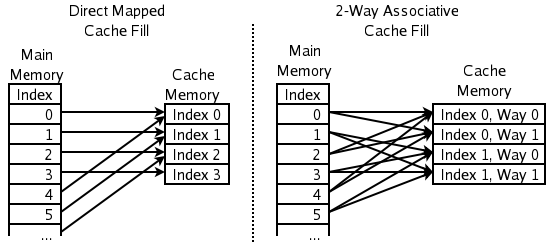
\includegraphics[width=0.8\textwidth]{basics/Cache_Asso.png}
\caption{Links ist ein direkt abgebildeter Cache zu sehen, bei dem die Hauptspeicheradresse den Cache-Index vollumfänglich festlegt. Rechts ist ein 2-Wege assoziativer Cache zu sehen bei dem etwa die Hauptspeicheradresse 0 sowohl auf \textit{Index 0, Way 0} als auch auf \textit{Index 0, Way 1} im Cache abgebildet werden kann \cite{CacheAssoWiki}.}
\end{figure}

%\newtextend

Der L3-Cache eines Intel i7-4770 ist beispielsweise 8 MiB groß und verfügt daher über 131072 ($2^{17}$) Cache-Einträge in der Größe einer Cache-Line. 
Wäre dieser Cache nun voll-assoziativ, müsste er bei jeder Anfrage komplett durchsucht werden. Aus diesem Grund ist der Cache in Cache-Sets unterteilt, wobei Daten einer spezifischen Hauptspeicheradresse nur in genau ein Cache-Set eingelagert werden können. 
Der i7-4770 besitzt 8192 dieser Cache-Sets, womit sich eine Assoziativität von 16 ergibt, das heißt man teilt die Anzahl der Cache-Einträge durch Anzahl der Cache-Sets. Dies bedeutet, dass die Suche nach den Daten einer Hauptspeicheradresse im Cache auf 16 Einträge begrenzt ist. 
%Die Zuordnung der physischen Hauptspeicheradressen zu den Cache-Sets ist nicht öffentlich dokumentiert.
Des Weiteren wird der Cache in \textit{Slices} unterteilt, wobei jede Slice einem Kern zugeordnet wird. Die Slices sind mittels eines Ringbuses verbunden, so dass jeder Kern auf Daten jeder Slice zugreifen kann. Die Zugriffslatenz erhöht sich mit der Anzahl der benötigten Hops, jedoch ist diese Erhöhung im Bereich von etwa 10 ns pro Hop. Diese Latenzunterschiede sind daher zu gering, um die Erkennung zwischen Cache-Hit und Cache-Miss zu gefährden, welche bei ca. 60 ns liegen \cite{TheSpyInTheSandbox}. Bei i7-4770 sind jedem der 4 Slices 2048 Cache-Sets zugeordnet. Die Zuordnung der Cache-Sets innerhalb der Slices sind fest an die untersten 18 Bit der pysischen Adresse gekoppelt. Zu welchem Slice ein Adresse gemappt wird, wird durch eine nicht dokumentierte Hashfunktion bestimmt.

%Im Rahmen dieser Arbeit sind Slices daher vernachlässigbar, so dass etwa bei Cache-Spezifikationen Slices nicht gesondert erwähnt werden.
%\todo[size=\footnotesize]{Eventuell Slices doch nicht so vernachlässigbar, da store forward eviction set Suche Slices einbezieht)}



%\todo[size=\footnotesize]{Hier fehlt wieder Mapping durch letzte Bits der Adresse (Beschrieben in Abschnitt Prime and Probe)}

%Ein CPU-Cache enthält mehrere Einträge, welche folgende Bestandteile besitzen:
%\begin{enum}
%\item Cache-Line: Die gecacheten Daten, wobei die Länge in der Core-Architektur etwa 64 Bytes beträgt.
%\item Address-Tag: Die Adresse im Hauptspeicher von der die Daten in der Cache-Line stammen.
%\item Flag-Bits: Etwa das "Dirty"-Bit welches anzeigt ob die Daten der Cache-Line noch mit denen im Hauptspeicher übereinstimmen.
%\end{enum}

\subsection{\textit{Inclusive} und \textit{exclusive}}
Ein Cache wird als \textit{inclusive} bezeichnet, falls alle Daten, die in einem niedrigen Cache-Level vorliegen, zusätzlich auch in den höheren Cache-Levels eingelagert sind. 
So besitzen die Caches aller Desktop-Versionen der Intel Core-Architektur diese inclusive-Eigenschaft (Stand Juni 2018).
Die Caches der Desktop-Prozessoren des Konkurrenten AMD haben zum Beispiel die Zen-Architektur \cite{CacheRyzen}, während jene der aktuellen Skylake-X-Prozessoren \cite{CacheSkylakeX} für Intels High-Performance-Plattform diese Eigenschaft hingegen nicht besitzen.
Wegen des großen Marktanteils von Intel-CPUs kann festgehalten werden, dass der Großteil der sich im Einsatz befindlichen Prozessoren mit \textit{Inclusive}-Caches ausgestattet ist.

\section{Cache-Angriffe}

Cache-Angriffe beschreiben eine generelle Klasse von Mikroarchitektur-Seitenkanalangriffen, welche den Cache verwenden, um Informationen abzugreifen, wobei der Cache als geteilte Ressource zwischen verschiedenen Prozessen fungiert. Durch diesen Angriff können sichere und unsichere Prozesse über den geteilten Cache trotz höher liegender Schutzmechanismen wie virtualisiertem Speicher oder Hypervisor-Systemen kommunizieren. 
Eine Angreiferin könnte ein Programm entwickeln, welches Informationen über den inneren Zustand eines anderen Prozesses sammelt, und so AES-Schlüssel \cite{BernsteinAES} sowie RSA-Schlüssel \cite{CacheAttackRSA} abgreifen auch über die Grenzen von virtuellen Maschinen hinweg.

%\newtext

\subsection{Flush and Reload}

Diese Angriffstechnik wurde 2014 von Yuval Yarom
und Katrina Falkner veröffentlicht \cite{FlushReload}.
Ausgang dieses Angriffs ist ein architekturspezifischer Flush-Befehl wie etwa der x86-Assemblerbefehl \textit{clflush}, welcher eine Adresse entgegennimmt und die dazugehörige Cache-Line invalidiert. 
Dadurch müssen die Daten beim nächsten Zugriff aus dem Hauptspeicher geladen werden. Dies ist die erste Phase des Angriffs und wird als Flush bezeichnet. 

Nach dem Flush folgt die Wait-Phase, in welcher die Angreiferin eine bestimmte Zeitperiode wartet und anschließend die Zugriffszeit auf die geflushte Adressse misst. 

Zu guter Letzt folgt die Reload-Phase, in welcher die Angreiferin auf die Adresse zugreift. Sofern das Opferprogramm in der Wait-Phase auf die Adresse zugegriffen hat, ist die Zugriffszeit gering, da die Daten bereits im Cache vorliegen.
Im anderen Fall müssen die Daten erst aus dem Hauptspeicher geladen werden, womit eine messbar erhöhte Zugriffszeit einhergeht \cite{FlushReload}. Eine Übersicht der eben beschriebenen Schritte als Pseudocode findet sich in Algorithmus \ref{alg:flush_and_reload}.

Ein Nachteil dieser Angriffsmethode ist die Notwendigkeit, dass sich der Opferprozess Speicherseiten mit dem Prozess der Angreiferin teilen muss. 
Ein typisches Beispiel hierfür sind geteilte Bibliotheken, zum Beispiel .so Dateien unter Linux oder .dll Dateien unter Windows, welche etwa Kryptofunktionen bereitstellen. Des Weiteren ist der clflush-Befehl nicht in jeder Umgebung verfügbar. So ist etwa ein Angriff aus dem Browser heraus mit dieser Methode nicht möglich. 
%\todo[size=\footnotesize]{Du hast ja schon geschrieben todo. Hier vielleicht auch eine kleine abbildung, aber defintiv irgendwas über flush WAIT reload und zeitmessungen}


%\todo{Ok, ich sehe du benutzt keine listing-Umgebung, sondern das alogrithm(2) Paket. Dann habe ich keine Ahnung, wie du die Schriftgröße anpassen kannst. Musst du dann selber rausfinden.}
\SetKwProg{Fn}{Function}{}{}

\begin{algorithm}[h]
\DontPrintSemicolon
\caption{Pseudo-Code für Flush and Reload}
\label{alg:flush_and_reload}
\SetAlgoNlRelativeSize{-2}

\Fn{$flushAndReload(address)$}{
    clflush(address)\;
    wait()\;
	timestampBefore <- getTimestamp()\;
	readMem(address)\;
	timestampAfter <- getTimestamp()\;
	\Return timestampAfter - timestampBefore > threshold
}

%\newtextend

\end{algorithm}

\subsection{Prime and Probe}

Ein erfolgreicher Prime and Probe Angriff auf den L3-Cache wurde 2015 von Liu et al. veröffentlicht \cite{LiuPrimeAndProbe}.
Er unterscheidet sich von Prime and Probe Angriffen auf niedrigere Cache-Level durch die aufwendigere Eviction-Set Suche.

Ein \textit{Eviction-Set} sei eine Menge Adressen, welche einen Cache-Eintrag aus einem Cache verdrängen kann. D.h. ein Eviction-Set, welches einen Eintrag aus dem L3-Cache löscht, würde den gleichen Zweck wie der \textit {clflush}-Assemblerbefehl im Flush-and-Reload-Angriff erfüllen. 
Um einen Eintrag aus dem Cache zu verdrängen, müssen mehrere Adressen der Daten aus dem Eviction-Set von der CPU auf das gleiche Cache-Set wie der zu verdrängende Eintrag abgebildet werden, so dass die Größe eines Eviction-Sets mindestens die Assoziativität des Caches erreichen muss.

Die Idee beim Prime and Probe Angriff besteht darin, in einer sich wiederholenden Abfolge zuerst den Cache zu primen, dann das Opferprogramm rechnen zu lassen und anschließend zu proben.
In der Priming-Phase werden mittels der Eviction-Sets gezielt Cache-Sets vollständig mit den Daten aus dem Eviction-Sets belegt.
In der anschließenden Berechnungsphase werden einige Einträge aus den geprimten Cache-Sets vom Opferprogramm verdrängt. Abschließend berechnet die Angreiferin die Summe der Zugriffszeiten auf alle Einträge in einem Eviction-Set.
Sofern das Opferprogramm in dem zum Eviction-Set korrelierenden Cache-Set Einträge verdrängt hat, kann die Angreiferin eine Abweichung nach oben in ihrer Messung feststellen, da die verdrängten Einträge eine erhöhte Zugriffszeit verursachen. Somit kann aus den Zugriffszeiten der Eviction-Sets auf die Speicherzugriffe des Opferprogramms geschlossen werden.

Die Eviction-Sets, die zur Durchführung eines Cache-Angriffs notwendig sind, lassen sich nicht immer leicht finden, da das Mapping der virtuellen auf die physischen Adressen in manchen Umgebungen nur eingeschränkt zugänglich ist.
So ist aber in der Regel das Mapping der virtuellen und physischen Adressen bei den Adressbits der Speicher-Pages identisch, welche etwa unter Windows und Linux zur Zeit 4096 Bytes groß sind. Somit ist in diesem Fall garantiert, dass die untersten 12 virtuellen Adressbits mit den physischen Adressbits identisch sind. 

%Der L3-Caches des Intel i7-4770 ist etwa 8 Mib groß, sodass 11 Bits des Mapping auf die physischen Adressen unbekannt sind.
%In solchen Fällen müssen die Eviction-Sets in einem Trial-and-Error-Verfahren ermittelt werden, wie es der Algorithmus TODO %\ref[alg:evictionSet} beschreibt.

\begin{algorithm}[h]
\DontPrintSemicolon
\caption{Psuedo-Code für Prime and probe}
\label{alg:prime_and_pribe}

\Fn{$flushAndReload(address)$}{
    \ForEach{address in evictionSet}{
        readMem(address)\;
    }
    wait()\;
	timestampBefore <- getTimestamp()\;
	\ForEach{address in evictionSet}{
        readMem(address)\;
    }
	timestampAfter <- getTimestamp()\;
	\Return timestampAfter - timestampBefore > threshold
}

\end{algorithm}


%Beschreibe Algorithmus
%Hierfür werden zuerst wiederholt Speicherblöcke angefordert, wobei solche in einer Menge gesammelt werden, welche 

%\newtext

\subsection{Timer}

Beide eben beschrieben Angriffsmethoden setzen voraus, dass die Angreiferin Laufzeitunterschiede zwischen dem Ladevorgang aus dem Cache und dem Hauptspeicher zuverlässig unterscheiden kann. Beim AIDA64-Benchmark mit einem aktuellen Intel i7-8700K ist die L3-Cache-Latenz im Mittel bei 12 ns, wobei gepaart mit DDR4-3200 CL16 RAM die Hauptspeicherlatenz im Mittel 49 ns beträgt \cite{i78700kLatency}. Somit ist eine Timer-Auflösung von unter 30 ns Voraussetzung für ein erfolgreichen Angriff. Anschaulich ist dies auch im Diagramm \ref{fig:RAMCacheLatency} zu sehen. Die Autoren verwendeten ein i7-4960HQ und haben Zugriffszeitdifferenzen für Cache-Miss und Hit von etwa 70 ns festgestellt. 

\label{fig:RAMCacheLatency}
\begin{figure}[h]
\centering
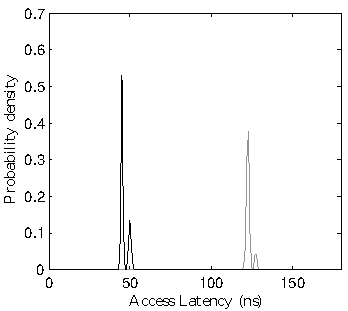
\includegraphics[width=0.55\textwidth]{basics/i7-4790HQ_latency_plot.pdf}
\caption{Wahrscheinlichkeitsverteilung der Zugriffszeiten für eine aus dem Cache verdrängte und dort vorliegende Variable \cite{TheSpyInTheSandbox}}
\end{figure}

\section{Chinesischer Restsatz}
\label{chinese_remainder}

Beschrieben sei ein System linearer Kongruenzen \cite{CRTref}:
\begin{align*}
x \equiv a_1 &(\mod m_1)\\
x \equiv a_2 &(\mod m_2)\\
\vdots\\
x \equiv a_3 &(\mod m_3)
\end{align*}
Für dieses System sollen alle $x$ bestimmt werden, welche alle Gleichungen erfüllen.
Wenn alle $m_1,m_2,...,m_n$ paarweise teilerfremde natürliche Zahlen sein, so existiert für jedes ganzahlige Tupel $a_1, ..., a_n$ genau eine Lösung $x \in \{0,1,...,kgV(m_1,m_2,...,m_n)\}$ \cite{CRTwiki}.

Sofern alle Moduli $m_i$ Primzahlen sind vereinfacht sich $kgV(m_1,m_2,...,m_n)$ zu $\prod_i m_i$.

Eine konkrete Lösung für $x$ ist etwa mit Hilfe des erweiterten euklidischen Algorithmus berechenbar.

\section{RSA}

RSA (Rivest–Shamir–Adleman) ist ein 1978 veröffentlichtes und weitverbreitetes Public-Key-Kryptosystem \cite{RSAPaper}.
Das grundlegende Prinzip hinter RSA ist es,  große positive natürliche Zahlen $e,d,n$ zu finden, so dass $(m^d)^e \equiv m \mod n$ gilt, aber schwer ein $d$ zu finden ist, wenn nur $e$ und $n$ gegeben sind.

Der RSA-Algorihtmus besteht aus vier Schritten: Der Schlüsselgenerierung, der Schlüsselverteilung, der Verschlüsselung und Entschlüsselung.

Für die Schlüsselgenerierung werden zwei Primzahlen $p$ und $q$ benötigt, und anschließend wird $n = pq$ berechnet. Die Länge $n$ wird auch als Schlüssellänge bezeichnet.

Eine heute gängige Schlüssellänge ist 2048 Bit, so dass die Bitlänge jeder Primzahl in etwa 1024 Bit beträgt. 
Um derart große Primzahlen in akzeptabler Zeit zu finden, werden probabilistische Primzahltests eingesetzt, welche mit einer hohen Wahrscheinlichkeit garantieren, dass die gefundenen Zahlen prim sind.

Des Weiteren wird $\lambda(n) = kgV(\lambda(p),\lambda(q)) = kgV(p-1, q-1)$ berechnet, wobei $\lambda$ die Carmichael-Funktion beschreibt.
Diese liefert zu jeder natürlichen Zahl $n$ die kleinste Zahl $\lambda(n)$, sodass $a^m \equiv 1 \mod n$ für jedes $a$ gilt.

Sei $e$ eine natürliche Zahl mit $1<e<\lambda(n)$ und teilerfremd zu $\lambda(n)$, d.h. es gilt $ggT(e,\lambda(n)) = 1$. Weiter sei $d \equiv e^{-1} \mod \lambda(n)$.

Im Rahmen dieser Arbeit liegt der Fokus darauf, während der Schlüsselgenerierung Informationen über die generierten Primzahlen p und q abzugreifen.

%\todo{verschlüsseln und entschlüsseln ist irrelevant für diese Arbeit. Statt es zu beschreiben einfach "im rahmen dieser Arbeit wurde versucht, während der Schlüsselgenerierung Informationen über die generierten Primzahlen p und q abzugreifen" oder so. Da wir jetzt ja ein "Idenifikation von Angriffszielen" kapitel haben, passt RSA vielleicht da besser statt in die Grundlagen}

%Der öffentliche Schlüssel besteht nun aus $n$ und dem Exponenten $e$ und muss Personen bekannt sein, welche Nachrichten verschlüsseln möchten.

%Um eine Nachricht $m$ mit $0 \leq m < n$ zu verschlüsseln, berechnet der Sender $c \equiv m^e \mod n$ mit dem $e$ aus dem öffentlichen Schlüssel des Empfängers und sendet den Chiffretext $c$ an den Empfänger.

%Der geheime Schlüssel ist der Exponent $d$, wobei die Zahlen $p,q,\lambda(n)$ ebenfalls geheim bleiben müssen, da andernfalls $d$ leicht berechnet werden könnte.

%Der Empfänger wiederum nutzt sein $d$ aus dem privaten Schlüssel, um $c^d \equiv (m^e)^d \equiv m \mod n$, die ursprüngliche Nachricht, zu berechnen.




%RSA Key Gen, RSA Verschlüsselung Entschlüsselung


\section{Javascript und Webassembly}

Javascript ist eine interpretierte Hochsprache, welche zusammen mit HTML und CSS die wichtigsten Komponenten für das World Wide Web bildet. 
Interaktive Webseiten und Applikationen werden erst mit Hilfe von Javascript möglich, weshalb jeder moderne Browser eine Javascript-Engine mitbringt.

Webanwendungen mit Javascript sollen auf unterschiedlichsten Endgeräten vom Laptop über das Smartphone bis zur Heimkonsole laufen, so dass ein Vorhalten von kompilierten Binärdateien für jedes dieser Geräte schwierig ist. 
Dennoch soll die Webanwendung beim Anwender ohne lange Ladezeiten auskommen, womit die Kompilierung auf dem Anwendungsgerät als Lösung entfällt.

Unter anderem deshalb ist Javascript eine interpretierte Sprache, welche jedoch ein Geschwindigkeitsnachteil gegenüber vorkompilierten Sprachen wie C oder Java hat.
Es wurden viele Anstrengungen unternommen, diesen designbedingten Performancenachteil auszugleichen. 
So erkennt etwa Googles Javascript-Engine V8 häufig genutzte, langsam laufende Codeteile und optimiert diese während der Laufzeit \cite{GoogleTurboFan}.

WebAssembly ist ein W3C-Webstandard, welcher ein binäres Format für ausführbaren Code in Webseiten definiert. 
Dieser Standard wurde 2017 ins Leben gerufen, um den Performancenachteil von Javascript gegenüber nativen Code zu reduzieren, sowie eim kompakte Code-Repräsentation zu bieten, und wird von allen gängigen Webbrowsern unterstützt.

Des Weiteren ermöglicht WebAssembly die Entwicklungen von Webanwendungen in anderen Sprachen wie etwa C, dessen Code abschließend in ein binäres Format, Wasm-Modul genannt, kompiliert wird.
Dieser ist aber weiterhin maschinenunabhängig, sodass nur ein Wasm-Modul vorgehalten werden muss.
Diese Module können von Javascript als Bibliotheken geladen und verwendet werden.

\section{Drive-by Attacks}

Die große Herausforderung eines Angriff auf ein Endgerät ist es, den Schadcode auf dem Gerät des Opfers zur Ausführung zu bringen. Eine beliebte Methode ist das so genannte Social-Engineering, welches darauf abzielt, bei Anwendern bestimmte Reaktionen wie etwa das Öffnen eines E-Mail-Anhangs hervorzurufen. Allerdings muss hier das Opfer selbst aktiv mitwirken, um dem Angriff zum Erfolg zu verhelfen.

Im Gegensatz dazu steht der Drive-by-Attack \cite{DriveByAttacksGeneric}, bei dem das Opfer bereits durch den Besuch einer Website angegriffen wird. Zum einen ist es möglich, durch Lücken im Browser beliebigen Code auf dem Gerät des Opfers auszuführen. Zum anderen, wie in der vorliegenden Arbeit dargestellt, können die vorhandenen Mittel wie Scriptsprachen für einen Angriff genutzt werden.
Die Erfolgswahrscheinlichkeit eines Angriffs ist im letzteren Fall bedeutend größer, da bereits die von der Angreiferin geschalteten Werbeanzeigen auf häufig aufgerufenen Webseiten für einen umfangreichen Pool von Opfern sorgen.
Hinzu kommnt, dass die meisten Opfer den Angriff nicht zu ihrem Ursprung zurückverfolgen können, da sie die Website mit der bösartigen Werbeanzeige regelmäßig besuchen.

Somit ist, zusammenfassend bemerkt, das Schreiben von Drive-by-Angriffen zunächst aufwändiger und setzt in der Regel die Kenntnis unbekannter oder nicht gepatchter Sicherheitslücken voraus, verspricht dafür aber eine deutliche höhere Erfolgswahrscheinlichkeit.

%Mit der zunehmenden Wandlung vieler Applikationen weg von der lokalen Desktopanwendung hin zur endgerätunabhängigen Webanwendung

%\todo[size=\footnotesize]{Fehlt: irgendwas in Richtung Drive-by, JIT-Environments, WebAssembly}

%\todo{was soll das ständige newtextend denn tun?}
%das markiert für nicht latex- beziehungsweise versionskontrollenaffine Nutzer farblich Textstellen die ich geändert habe
%\newtextend

\section{Speicher-Disambiguierung}

Heutige Prozessoren, wie etwa die Intel-Core-Reihe, führen Store- und Load-Befehle Out-of-Order aus und stehen damit vor der Aufgabe, auf Datenabhängigkeiten 
%(Was ist das denn?) In diesem Kontext klar
zu reagieren \cite{memoryDisambiguationBlog}.
Die Techniken für eine Speicher-Disambiguierung erkennen echte Abhängigkeiten zwischen Speicheroperationen während der Ausführung und erlauben es der CPU, zu einem vorherigen Zustand zurückzukehren, sobald eine Abhängigkeit verletzt wurde.

Die Möglichkeit, Load- und Store-Befehle Out-of-Order auszuführen, sorgt für eine erhöhte Parallelität auf Instruktionsebene und eine damit verbesserte Single-Thread-Performance.
Grafik \ref{fig:MemoryDisambiguation} zeigt ein Beispiel für die Speicher-Disambiguierung. 

\label{fig:MemoryDisambiguation}
\begin{figure}[h]
\centering
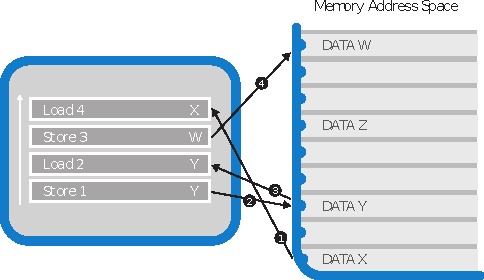
\includegraphics[width=0.6\textwidth]{methods/memory_disambiguation.pdf}
\caption{Beispiel für eine Speicher-Disambiguierung. Die Nummern in den Kreisen geben die chronologische und der weiße Pfeil am linken Rand die logische Ausführungsreihenfolge an. Load 2 kann nicht früher ausgeführt werden, da er von Store 1 abhängig ist. Load 4 hingegen ist von den anderen Operationen unabhängig und kann daher vor Store 1 und Store 3 ausgeführt werden. Durch diese vorgezogene Ausführung können Instruktionen, die den Wert von X benötigen, im Folgenden von einer geringen Zugriffslatenz profitieren. \cite{CacheAssoWiki}.}
\end{figure}

Um diese Techniken umzusetzen, werden Store-Instruktionen bei der Ausführung nicht direkt an das Speichersystem, in diesem Fall den CPU-Cache, übermittelt.
Stattdessen werden die Store-Instrukionen inklusive der Speicheradressen und Daten in einer Store-Queue gepuffert.
Die Werte werden erst an das Speichersystem übergeben, wenn alle vorherigen Befehle im Code komplett abgeschlossen wurden.
Dies vermeidet Write-after-Read(WAR)-Konflikte, bei denen ansonsten ein früheres LOAD einen inkorrekten Wert vom Speichersystem lesen würde, weil die Ausführung eines späteren STORES vorgezogen wurde.
Auch Write-after-Write(WAW)-Konflikte werden dadurch gelöst, da keine früheren STORES ihre Werte nach späteren STORES in das Speichersystem übermitteln, wie es ohne STORE-Queue bei der Out-Of-Order-Ausführung der Fall wäre. 

Des Weiteren ermöglicht die Store-Queue die spekulative Ausführung von bedingten Verzweigungen, deren Richtung zum Ausführungszeitpunkt noch nicht bekannt ist.
Wenn ein Pfad falsch geraten wurde, muss der berechnete Pfad verworfen und alle STORES rückabgewickelt werden.
Ohne die Store-Queue wäre dies nicht möglich, da in der Zwischenzeit die geschriebenen Werte von anderen Cores gelesen sein könnten und somit der Systemzustand korrumpiert wäre.

Jedoch schafft die Store-Queue auch ein neues Problem.
Angenommen ein STORE wird ausgeführt und seine Adresse und seine Daten werden in der Store-Queue gepuffert. Kurz danach liest ein LOAD von derselben Adresse, auf die der STORE geschrieben hat.
Würde der LOAD den Wert vom Speichersystem lesen, wäre der Wert veraltet, da der im Code vorher stehende STORE noch nicht übermittelt wurde.

Um diesem Problem zu begegnen, nutzten Prozessoren in der Store-Queue die store-to-load-forwarding-Technik.
Diese veranlasst die Store-Queue, abgeschlossene STORES, die noch nicht an den Speicher übermittelt wurden, zu späteren LOADS weiterzuleiten.
Bei der Ausführung eines LOADS wird die als assoziativer Speicher umgesetzte Store-Queue nach STORES auf derselben Adresse durchsucht, welche in der logischen Ausführungsreihenfolge vorher auftauchen.
Sofern es einen Treffer gibt, wird der Wert des abgeschlossenen STORES aus der Store-Queue anstatt des veralteten Wertes aus dem Speichersystem verwendet.

\section{Angegriffene Hardware und Software}

Der Testrechner war ein Dell Precision T1700 mit einem Intel Core i7-4770, dessen 4 physischen Kerne beziehungsweise 8 virtuellen Kerne einen Grundtakt von 3,4GHz bieten.
Der geteilte L3-Cache ist 8 MiB groß, besitzt eine Assoziativität von 16, eine Cache-Line-Größe von 64 Byte und 8192 Cache-Sets, die in 4 Slices aufgeteilt sind.
Weiterhin ist ein Intel C226 Chipsatz und 8GB DDR3-1600 verbaut. 
Als Betriebsystem wird Ubuntu 16.04.5 LTS (GNU/Linux 4.4.0-131-generic x86_64) verwendet. 

Als Browser wurden Chromeium TODO, Firefox 62 sowie Firefox Developer Edition 63 getestet.


%Nuc i3-5... 2C4T, 

Mozilla Network Security Services(NSS) \cite{MozillaNSS} ist eine Menge von Bibliotheken, welche eine plattformübergreifende Entwicklung von sicheren Client- und Server-Anwendungen anstrebt. Dabei wird unter anderem TLS oder S/MIME implementiert. Mozilla NSS wird etwa im Firefox-Browser und der Mail-Anwendung Thunderbird eingesetzt.
Der Quellcode ist unter der Mozilla Public License verfügbar und kann online etwa im Firefox-Repository \cite{MozillaDXR} eingesehen werden.

OpenPGP ist ein Standard für das Signieren, Ver- und Entschlüsseln von Daten, welcher im RFC 4880 \cite{rfc4880} definiert wird.
OpenPGP.js \cite{OpenPGPjs} ist eine Opensource-Implementierung des OpenPGP-Protokolls in Javascript, welche sich zum Ziel gesetzt hat, OpenPGP auf einer breiten Palette (meinst du "Palette"?) von Endgeräten zu ermöglichen.
So wird OpenPGP.js etwa vom E-Mail-Dienst Protonmail \cite{Protonmail} genutzt.

%\todo{Besser in Implementierung aufgehoben?}
  \chapter{Implementierung}
\label{chapter:preparation}

\SetKwProg{Fn}{Function}{}{}

Das folgende Kapitel beschreibt, mit Hilfe welcher Softwaretools der Cache-Angriff implementiert wird.

In dem in dieser Arbeit verwendeten praxisnahen Angriffsmodell reicht für den Start eines Angriffs der Besuch des Opfers auf einer vorher präparierten Website, auch Drive-By-Angriff genannt, aus. 
Dafür genügt bereits eine eingebundene JavaScript-Werbeanzeige, die von der Angreiferin kontrolliert wird. 
Gegenüber Angriffen, die ein Ausführen von nativem Code auf dem Endgerät des Opfers verlangen, ist mit diesen Voraussetzungen ein deutlich größerer Angriffsvektor gegeben.
Da aufgrund des Angriffsmodells nur Webtechnologien verfügbar sind, liegt der komplette Angriffscode in JavaScript und Webassembly vor. 
Frühere Implementierungen von Cache-Angriffen im Browser \cite{TheSpyInTheSandbox} hatten noch keine Möglichkeit, Webassembly zu verwenden, weshalb deren kompletter Angriffscode in JavaScript geschrieben war. 
Webassembly ermöglicht hardwarenähere Programmierung und den Vorteil, dass der Code anders als in JavaScript nicht während der Laufzeit optimiert werden muss. 
Des Weiteren steht mit dem Emscripten-Compiler ein Tool bereit, welches die Übersetzung von C-Code in Webassembly anbietet. Somit kann ein bestehender Angriffscode in C, in diesem Fall von Mastik \cite{Mastik}, als Grundlage verwendet werden, und eine komplette fehleranfällige Neuimplementierung in JavaScript entfällt.

\section{Timer in JavaScript}

Der hier ausgeführte Cache-Angriff benötigt, wie im Grundlagenkapitel beschrieben, präzise Timer, welche eine Auflösung von unter 30 ns bereitstellen sollten. Dennoch könnte die Suche nach \textit{Eviction-Sets} auch mit schlechteren Timerauflösungen bewerkstelligt werden, indem Operationen mehrfach ausgeführt werden und die Differenz der aufsummierten Zeiten zur Bewertung herangezogen wird.
Im \textit{Eviction-Set}-Algorithmus könnte etwa die Funktion $checkevict$ wie in Algorithmus \ref{alg:checkevict_low_resolution} angepasst werden, wobei der Parameter $repeatIterations$ abhängig von der Timerauflösung gewählt wird. 
Es besteht jedoch das Problem, auch schwache Aktivitäten im Cache-Set während des eigentlichen Angriffs aufzudecken, da im Worst-Case nur ein Eintrag aus dem beobachteten Cache-Set verdrängt wird und somit lediglich die Zugriffszeit zwischen einem Hit und einem Miss ausschlaggebend ist. 
In diesem Fall könnte die Dauer mehrerer Prime-and-Probe-Iterationen gesamtheitlich gemessen werden, und zwar unter der Vermutung, dass auf die für die Verdrängung verantwortliche Adresse über die Zeit mehrfach zugegriffen wird.
Aus einem niedrig aufgelösten Timer folgt also eine geringere zeitliche Auflösung von Cache-Aktivitäten oder die Nichtregistrierung von schwachen Cache-Aktivitäten.

\begin{algorithm}[h]
\DontPrintSemicolon
\caption{Pseudo-Code für $checkevict$ im Fall von einer niedrig aufgelösten getTimestamp}
\label{alg:checkevict_low_resolution}

\Fn{$checkevict(possibleEvictionSet, witness)$}{
    timestampBefore <- getTimestamp()\;
    \For{i=1 to repeatIterations}{
        accessMemory(possibleEvictionSet)\;
        accessMemory(witness)\;
    }
	timestampAfter <- getTimestamp()\;
	\Return timestampAfter - timestampBefore > threshold
}

\end{algorithm}

Der W3C hat die High-Resolution-Time-API spezifiziert, welche die Methode performance.now beinhaltet, die einen aktuellen Timestamp zurückgibt. Im Firefox hatte die Methode in früheren Versionen eine hinreichend genaue Auflösung im Nanosekundenbereich, wobei in Reaktion auf die Sicherheitslücken Meltdown und Spectre die Auflösung schrittweise auf 2 ms im aktuellen Firefox 60 abgesenkt wurde. 
Auch in den Browsern Edge und Chrome wurden im Zuge der Veröffentlichung von Meltdown und Spectre die Auflösung von perfomance.now() verringert.
Darüber hinaus wird bei beiden Browsern auf den zurückgegebenen Timestamp ein Timerjitter addiert.

So bieten Edge und Chrome zurzeit (Stand Juni 2018) eine Auflösung von 20 \textmu s + 20 \textmu s Jitter respektive 100 \textmu s + 100 \textmu s Jitter.
Das Paper "Fantastic Timers and where to find them" \cite{FantasticTimers} beschreibt diverse andere Methoden, um mit Hilfe von JavaScript Timer zu generieren. 
Es werden etwa CSS-Animationen und Nachrichtenkanäle als mögliche Zeitgeber untersucht.
Allerdings ist nur eine geeignete Methode dabei, da die Auflösung aller anderen mindestens im hohen einstelligen \textmu s Bereich liegt und somit der Parameter $repeatIterations$ auf Werte von etwa 1000 gesetzt werden müsste, um zuverlässig \textit{Eviction Sets} zu finden. 
Hierdurch würde die benötigte Ausführungszeit zum Finden der \textit{Eviction Sets} auf ein Maß ansteigen, welches nicht mehr zum angenommenen Angriffsmodell passen würde.

%\newtext

Als einziges angemessenes Zeitmessungswerkzeug verbleibt der SharedArrayBuffer aus Javascript. 
Die Ausführung von Javascript geschieht in einem Thread, wobei die Möglichkeit besteht, so genannte Webworker zu starten, welche Code aus einem Skript in einem eigenen Thread ausführen.
Der Speicherbereich eines Webworkers und des Mainthreads sind strikt getrennt, sodass Daten ursprünglich über Nachrichten ausgetauscht werden mussten. Hier setzt der SharedArrayBuffer an, welcher einen geteilten Speicherbereich zwischen Mainthread und Webworker definiert.

Gemäß Code-Listing \ref{alg_list:sharedArrayBufferWorkerMain} wird im Mainthread zuerst ein SharedArrayBuffer von 4 Bytes angelegt. Anschließend wird der als Zeitgeber fungierende Webworker gestartet und ihm eine Referenz auf den eben angelegten SharedArrayBuffer übersandt. 

\begin{figure}[h]
\begin{lstlisting}[caption=main.js: Code für Zeitmessungen mittels counterWorker,label=alg_list:sharedArrayBufferWorkerMain]
var sharedArrayBuffer = new SharedArrayBuffer(4);
var counterWorker = new Webworker('counterWebworker.js');
counterWorker.postMessage(sharedArrayBuffer);
var sharedArrayBufferUin32Array = new Uint32Array(sharedArrayBuffer);

function measureTime(func){
    var t1 = Atomics.load(sharedArrayBufferUin32Array[0]);
    func();
    var t2 = Atomics.load(sharedArrayBufferUin32Array[0]);
    return t2 - t1;
}
\end{lstlisting}
\end{figure}

Die Zählvariable soll hier eine Größe von 32 Bits haben, weshalb abschließend ein \lstinline{Uint32Array} definiert wird, dessen Inhalt auf den SharedArrayBuffer referenziert. 
Ein Zählvariable kann nun durch Lesen des ersten Eintrags des Arrays erhalten werden. 
Problematisch ist jedoch, dass auf die Zählvariable sowohl lesend vom Mainthread als auch schreibend vom Webworker zugegriffen wird. 
Dadurch können die im Mainthread gelesenen Werte veraltet sein, da der SharedArrayBuffer noch nicht zwischen beiden Threads synchronisiert wurde. 
Abhilfe schafft hier die von Javascript bereitgestellte Atomics-Library, welche es ermöglicht, die Leseoperation atomar auszuführen.

Der Webworker iteriert nun in einem eigenen Thread die Zählvariable in einer Endlosschleife (siehe auch Pseudocode \ref{alg_list:sharedArrayBufferWorker}). 
Zuerst wird dazu dem Webworker via message die Referenz auf einen im Mainthread erstellten SharedArrayBuffer übergeben.
Anschließend wird im Webworker ein \lstinline{Uint32Array} angelegt, welches mit dem übergebenen SharedArrayBuffer verknüpft ist. 
Zum Schluss geht der Webworker in die Endlosschleife über, in welcher die Zählvariable \textit{sharedArray[0]} durchgehend iteriert.

\begin{figure}[h]
\begin{lstlisting}[caption=counterWebworker.js: Iterieren der Zählvariable in einer Endlosschleife mittels Webworker,label=alg_list:sharedArrayBufferWorker]
self.addEventListener('message', (m) => {
  // Create an Uint32Array on top of the shared memory array 
  const sharedArray = new Uint32Array(m.data);
  while{true}{
    sharedArray[0]++;
  }
});
\end{lstlisting}
\end{figure}

Das Iterieren einer Variable benötigt nur wenige Taktzyklen, wodurch der aktuelle Wert der Zählvariable als Zeitstempel interpretiert werden kann. 
Die Auflösung dieser Methode hängt also von der Geschwindigkeit der Iteration sowie der Speichersynchronisation des SharedArrayBuffers zwischen Mainthread und Webworker ab.

In Versuchen mit verschiedenen Webbrowsern und Hardwarekonfigurationen zeigte sich, dass die Auflösung mindestens im einstelligen Nanosekundenbreich liegt und somit ausreichend genau ist, um den Unterschied zwischen einem Cache-Miss und Hit festzustellen (siehe Tabelle \ref{tbl:times_res}).

Um die Auflösung zu bestimmen, wird die Javascriptfunktion performance.now zur Hilfe genommen (siehe Listing \ref{alg_list:getResolutionNS}). Die Funktion \lstinline{wait_edge} ruft zuerst performance.now für den Startwert auf und wartet anschließend in einer Endlosschleife, bis performance.now einen höheren Wert als den Startwert zurückgibt. 
Dieser höhere Wert wird ebenso wie der aktuelle Stand der Zählvariable gespeichert. 
Dann folgt ein erneuter Aufruf von \lstinline{wait_edge}, wobei beim Zurückkehren wieder der letzte performance.now-Wert sowie der Wert der Zählvariable gespeichert wird.
Für die performance.now-Funktion ist die Auflösung bekannt, sodass aus den Differenzen der performance.now-Werte und der Werte der Zählvariable eine Auflösung für den Timer errechnet werden kann.
Wie oben beschrieben addiert Chrome auf den performance.now-Wert einen Timerjitter, und deshalb wurde diese Prozedur 20000 mal durchgeführt, um valide Mittelwerte zu erhalten.

Die Zählvariable besitzt den Datentyp \lstinline{Uint32}, und in Javascript ergibt eine Iteration des Wertes $2^{32}-1$ wieder 0. 
Daher ist es naheliegend, den gesamten Wertebereich von 0 bis $2^{32}-1$ auszuschöpfen und bei Messwerten über $2^{31}$ anzunehmen, dass in diesem Zeitraum ein Overflow stattfand.
Beim Testen mit Firefox zeigte sich jedoch, dass die Iteration der Zählvariable ab dem Wert $2^{31}$ signifikant langsamer wird, wobei dieses Phänomen mit Chrome nicht zu beobachten war.
Als Workaround wurde eine Abfrage hinzugefügt, die bei einem Überschreiten von $2^{31}$ die Zählvariable auf 0 zurücksetzt.
Die Ergebnisse zeigen, dass dieser Workaround die Auflösung in Chrome nur minimal verschlechtert, dafür aber in Firefox signifikant verbessert.
Ohne diese Änderungen sorgt der Timer in Firefox für Probleme bei der Zeitmessung, da ein Zeitintervall beim Überschreiten des Wertes $2^{31}$ wegen der verringerten Iterationsgeschwindigkeit als deutlich verkürzt wahrgenommen wird.

\begin{table}[h]
\caption{Zeitauflösung des SharedArrayBuffer-Zählers mit verschiedenen Browsern auf Ubuntu 16.04.5 LTS (GNU/Linux 4.4.0-131-generic x86_64) mit einem i7-4770. Wertebereich der \lstinline{Uint32} Zählvariable wird in der linken Spalte ausgeschöpft, in der rechten hingegen wird nur bis $2^{31}$ gezählt.}
\label{tbl:times_res}
\begin{tabular}{lllll}
\toprule
                           & Zählen bis $2^{32}$ & Zählen bis $2^{31}-1$ &  &  \\
                           \midrule
Chromium 68.0.3440.106     & $\sim$2,7ns                      & $\sim$3ns                        &  &  \\
Google Chrome 69.0.3497.81 & $\sim$2,7ns                      & $\sim$3ns                        &  &  \\
Firefox 63.0b4             & $\sim$5,1ns                      & $\sim$2,2ns                      &  &  \\
\bottomrule
\end{tabular}
\end{table}


\begin{figure}[h]
\begin{lstlisting}[caption=main.js: Code zur Bestimmung der Timerauflösung,label=alg_list:getResolutionNS]
var start = wait_edge();
var start_count = Atomics.load(Module['sharedArrayCounter'], 0);
var end = wait_edge();
var end_count = Atomics.load(Module['sharedArrayCounter'], 0);
nsPerTick += (end - start) * 10^6 / (end_count - start_count);

function wait_edge() {
  var next, last = performance.now();
  while ((next = performance.now()) == last) {}
  return next;
}
\end{lstlisting}
\end{figure}

Diese Methode geht allerdings mit dem Nachteil einher, dass der Webworker-Thread in der Messphase einen CPU-Kern komplett auslastet. Das heißt, dass im Angriffsszenario das Opferprogramm, der Javascript-Mainthread und der Webworker gleichzeitig rechnen, sodass mindestens 3 CPU-Kerne benötigt werden. 
Sofern sich der Webworker einen physischen Kern mit einen anderen aktiven Prozess teilt, können die gemessen Zeiten einer stärkeren Volatilität durch die erhöhte Iterationsdauer unterliegen.
Folglich reduziert sich die Auflösung des Zeitgebers, wobei eine ausreichende Genauigkeit dennoch gegeben ist, da beide Prozesse in etwa die gleiche Rechenzeit zugesprochen bekommen.

Aufgrund der Option, den SharedArrayBuffer als Timer zweckzuentfremden, wurde dieser im Zuge der Veröffentlichung von Meltdown und Spectre in allen gängigen Webbrowsern deaktiviert \cite{FirefoxSharedArrayBuffer}. Jedoch planen die Hersteller, das Feature in Zukunft wieder zu aktivieren, sobald die Gefahr von Angriffen wie Meltdown und Spectre reduziert ist. 
Google ist der erste Hersteller, der in seinem Chrome-Browser mit Version 68 die SharedArrayBuffer wieder aktiviert hat \cite{ChromeSharedArrayBufferAgain}. 
Als logische Konsequenz wurde angekündigt, in Zukunft erneut hochauflösende Timer bereitzustellen, da ein SharedArrayBuffer genau diese Möglichkeit schon jetzt bereitstellt \cite{ChromeHighResolutionTimerAgain}.

Aus diesen Gründen wird im Folgenden davon ausgegangen, dass das Opfer SharedArrayBuffer in seinem Webbrowser aktiviert hat.

%\todo{Hier steht ein h in eckigen Klammern. Listings funktionieren nicht so, das sind keine float-umgebungen. Darum bricht auch mitten im Listing die Seite um. Um es "hübsch" in den text einzufügen musst du das listing in eine figure packen. Ansonsten taucht es einfach immer genau da auf, wo du es hinsetzt.}

%moved from section grundlagen
\section{Eviction-Set-Algorithmus in der Javascript-Umgebung}
%\section{Cache-Angriff in JavaScript und Webassembly}
Der wichtigste Teil für einen Prime-and-Probe-Angriff ist die Fähigkeit, zuverlässig Eviction-Sets zu finden. Wie im Grundlagenkapitel beschrieben, führt die CPU das Cache-Mapping anhand der physischen Adressen durch. Webassembly emuliert eine 32-Bit-Umgebung, welche die internen Adressen in virtuelle Adressen des Hostprozesses, hier des Browsers, übersetzt. 
Webassembly-Code verwendet nur Adressen der emulierten Umgebung und hat keinerlei Zugriff auf das Mapping zu den virtuellen Adressen. 

Somit sind die physischen Adressen in Webassembly durch gleich zwei Abstraktionsschichten geschützt. 
Jedoch lässt sich für das Finden der Eviction-Sets die Eigenschaft ausnutzen, dass im Betriebssystem 4-KiB-Pages existieren, sodass die letzten 12 Bits der virtuellen und physischen Adresse identisch sind. 
Des Weiteren alloziert %(??? erstellt?) hier der Fachausdruck
Webassembly 4 KiB große Blöcke, die zur Übereinstimmung der 12 letzten Bits der Webassembly-Adresse mit der virtuellen und physischen führen.

Um aus dieser Eigenschaft Kapital zu schlagen, wird ein Array angelegt, der mindestens die Größe des L3-Caches in Webassembly hat. Im Folgenden soll der Intel i7-4770 mit 8 MiB großem L3-Cache erneut als Basis dienen. In diesem Array sind nun $x$ Blöcke der Größe 4 KiB, deren letzte 12 Adressbits mit der physischen Adresse übereinstimmen. Im sogenannten Adresspool seien nun die Adressen des Arrays, bei denen die letzten 12 Bits gleich sind, also insgesamt $x$ Stück.

Der i7-4770 besitzt 8192 Cache-Sets, die auf 4 Slices aufgeteilt sind, wobei für das Mapping der 2048 Cache-Sets innerhalb eines Slices nur die untersten 17 Bits der physischen Adresse relevant sind (siehe auch Abbildung \ref{fig:address_layout}. Dabei bestimmen die Bits 6 bis 17 eindeutig das Cache-Set und die Bits 0 bis 5 das Offset innerhalb der Cache-Line.

\label{fig:address_layout}
\begin{figure}[h]
\centering
\begin{scaletikzpicturetowidth}{\textwidth}
\begin{center}














\end{center}


\tikzset{every picture/.style={line width=0.75pt}} %set default line width to 0.75pt        

\begin{tikzpicture}[x=0.75pt,y=0.75pt,yscale=-1,xscale=1]
%uncomment if require: \path (0,147); %set diagram left start at 0, and has height of 147

%Shape: Rectangle [id:dp378127113165748] 
\draw   (139.4,25) -- (399,25) -- (399,50) -- (139.4,50) -- cycle ;
%Shape: Rectangle [id:dp46142039984044336] 
\draw   (139.8,64) -- (444,64) -- (444,89) -- (139.8,89) -- cycle ;
%Shape: Rectangle [id:dp8338046143479867] 
\draw   (399,25) -- (487,25) -- (487,50) -- (399,50) -- cycle ;
%Shape: Rectangle [id:dp940182630841411] 
\draw   (487,25) -- (545,25) -- (545,50) -- (487,50) -- cycle ;
%Shape: Rectangle [id:dp12367960229267094] 
\draw   (444,64) -- (545,64) -- (545,89) -- (444,89) -- cycle ;
%Shape: Rectangle [id:dp7768353739474505] 
\draw   (315,106) -- (545.33,106) -- (545.33,131) -- (315,131) -- cycle ;
%Straight Lines [id:da18312510628843603] 
\draw  [dash pattern={on 0.84pt off 2.51pt}]  (443.9,105.6) -- (443.9,129.6) ;



% Text Node
\draw (721,21) node   {$0$};
% Text Node
\draw (701,71) node   {$0$};
% Text Node
\draw (67,37) node  [align=left] {Phyische Adresse};
% Text Node
\draw (71,76) node  [align=left] {Virtuelle Adresse};
% Text Node
\draw (75,120) node  [align=left] {Webassambly's\\ \ \ \ \ \ Adresse};
% Text Node
\draw (516,38) node [scale=0.7] [align=left] {Cache-Line\\ \ \ \ Offset};
% Text Node
\draw (443,38) node [scale=1] [align=left] {Cache-Set};
% Text Node
\draw (266,38) node [scale=1] [align=left] {Slice (durch Hashfunktion)};
% Text Node
\draw (141,16) node [scale=0.7] [align=left] {64};
% Text Node
\draw (400,17) node [scale=0.7] [align=left] {17};
% Text Node
\draw (488,16) node [scale=0.7] [align=left] {6};
% Text Node
\draw (546,16) node [scale=0.7] [align=left] {0};
% Text Node
\draw (298,76) node [scale=1] [align=left] {Page};
% Text Node
\draw (495,77) node [scale=1] [align=left] {Page Offset};
% Text Node
\draw (445,57) node [scale=0.7] [align=left] {12};
% Text Node
\draw (316,98) node [scale=0.7] [align=left] {32};
% Text Node
\draw (546,56) node [scale=0.7] [align=left] {0};
% Text Node
\draw (546,98) node [scale=0.7] [align=left] {0};
% Text Node
\draw (445,98) node [scale=0.7] [align=left] {12};
% Text Node
\draw (432,118) node [scale=1] [align=left] {Adressbits};


\end{tikzpicture}
\begin{center}


\end{center}

\end{scaletikzpicturetowidth}
\caption{Physischer, virtueller und Webassembly's Adressraum auf dem Intel i7-4770 mit vier Slices und insgesamt 8192 Cache-Sets im Vergleich \cite{DriveByPaper}. Die letzten 12 Bits einer Adresse stimmen in allen drei Adressräumen überein.}
\end{figure}

In welchem der 4 Slices die Daten landen, wird anhand der Adressbits 18 bis 63 bestimmt.
Durch die Kenntnis der untersten 12 Bits der physischen Adresse sind gleichzeitig 6 Bits (6 bis 11) bekannt, welche für die Zuordnung zu den Cache-Sets verantwortlich sind.

Angenommen, im Pool sind ausschließlich Adressen, bei denen die letzten 12 Bits auf 0 gesetzt sind. 
Somit ist ein Abstand von $2^{12}$ für aufeinanderfolgende Adressen gegeben und jede Adresse lässt sich genau einem der 4-KiB-großen Blöcke zuordnen.
Dann kann erwartet werden, dass im Mittel jede 128. 
Adresse auf das gleiche Cache-Set gemappt wird. Es gibt 8192 Möglichkeiten, eine Adresse einem Cache-Set zuzuordnen, also 13 Bits an Unsicherheit.
Durch die Kenntnis der untersten 12 Bits der Adresse sind davon 6 Bits bekannt, welche für eine eindeutige Zuordnung sorgen. 
Es bleiben noch 7 Bits an Unsicherheit, die durch Kenntnis der restlichen Adressbits beseitigt werden könnten.

\subsection{Eviction-Set-Suchalgorithmus}
\label{evictionSetSearchAlgo}

Im Folgenden soll der Algorithmus beschrieben werden, der die Adressen im Pool verschiedenen Eviction-Sets zuordnet.
Dieser Algorithmus ist in der Lage, Adressen Cache-Sets zuzuordnen, ohne Näheres über die CPU (L3-Cache Größe usw.) und die Adressbits 12 bis 63 zu wissen.
Der Algorithmus basiert auf den von \cite{DriveByPaper} und \cite{PrimeAndAbort} beschriebenen Algorithmen zum Finden von Eviction-Sets, wobei einige Optimierungen und Modifikationen implementiert und getestet wurden.

Der Eviction-Set-Konstruktionsalgorithmus besteht aus drei Hauptphasen, der Expand-, Contract- und Collect-Phase. 
Zu Anfang wird zufällig eine Zeugenadresse aus dem Adresspool ausgewählt.
Die Annahme in der Expand-Phase ist, dass eine bestimmte Teilmenge der Adressen aus dem Pool, genannt Candidate-Set, ein Eviction-Set für die Zeugenadresse bildet, sofern der Pool groß genug ist. 
Um ein Candidate-Set zu testen, wird zuerst auf die Zeugenadresse zugegriffen, um sicherzustellen, dass diese im Cache landet.
Danach wird auf alle Adressen aus dem Candidate-Set zugegriffen und abschließend die Zugriffszeit auf die Zeugenadresse gemessen. 
Sofern das Candidate-Set ein Eviction-Set für die Zeugenadresse ist, werden die Daten der Zeugenadresse aus dem Cache verdrängt, womit bei einer erneuten Messung der Zeugenadresse eine erhöhte Zugriffszeit gemessen wird.
Dieser Vorgang wird mehrmals wiederholt, um den Einfluss des Timer- und System-Rauschens zu vermindern.

In der Expand-Phase wird dem Addresspool iterativ eine zufällige Adresse entnommen, welche in dieser Iteration die Zeugenadresse ist (siehe auch Pseudocode \ref{alg:evictionSetExpand}).
Nach jeder Iteration wird, wie eben beschrieben, getestet, ob das Candidate-Set ein Eviction-Set für die Zeugenadresse ist.
Falls dies zutrifft, wird zur nächsten Phase übergegangen, andernfalls wird die Zeugenadresse dem Candidate-Set hinzugefügt und mit der nächsten Iteration fortgefahren.

\begin{algorithm}[h]
\DontPrintSemicolon
\caption{Pseudo-Code für Expand-Phase des Eviction-Set Algorithmus}
\label{alg:evictionSetExpand}

\Fn{$Expand(evictionSet, addressPool)$}{
	\While{size(addressPool) > 0}{
		witness = SelectRandomItem(addressPool)\;
		\If{checkevict(evictionSet, witness)}{
			\Return witness
		}
		evictionSet.add(witness)\;
	}
	\Return failed
}
\end{algorithm}

Im Allgemeinen beinhaltet das Candidate-Set nach der Expand-Phase mehrere hundert Einträge, von denen eine Teilmenge der Größe 16 bereits ein Eviction-Set für die Zeugenadresse bilden würde. 
Der überwiegende Teil der Einträge gehört nicht zum gleichen Cache-Set wie die Zeugenadresse.
Diese überflüssigen Einträge würden den Prime-and-Probe-Vorgang erheblich verlangsamen. Deshalb wird in der Contract-Phase versucht, das Candidate-Set auf die Größe 16 zu reduzieren (siehe auch Pseudocode \ref{alg:evictionSetContract}).
Hierzu wird ein Element aus dem Candidate-Set entfernt und dann erneut getestet, ob dieses reduzierte Candidate-Set noch ein Eviction-Set für die Zeugenadresse ist.
Falls ja, wird dieses Element wieder dem Adresspool hinzugefügt, andernfalls verbleibt es im Candidate-Set, da es notwendiger Bestandteil des Eviction-Sets ist.
Dieser Vorgang wird für jedes Element im Candidate-Set einmal durchgeführt, so dass im fehlerfreien Fall schlussendlich 16 Elemente im Candidate-Set verbleiben.
Durch Messrauschen kann auch hier wieder ein Element fälschlicherweise als relevant für das Eviction-Set eingestuft werden, weshalb die Contract-Phase dreimal wiederholt wird.
Die zweite und dritte Wiederholung sind weit weniger kostenintensiv, da das Candidate-Set nach einer Contract-Phase bereits um mehrere 100 Einträge bereinigt wurde.

\begin{algorithm}[h]
%\algsetup{linenosize=\small}
\DontPrintSemicolon
\caption{Pseudo-Code für Contract-Phase des Eviction-Set Algorithmus}
\label{alg:evictionSetContract}
\Fn{$Contract(evictionSet, addressPool, witness)$}{
	\ForEach{candidate in evictionSet}{
	    evictionSet.remove(candidate)\;
		\If{checkevict(evictionSet, witness)}{
			addressPool.add(candidate)\;
		}\Else{
		    evictionSet.add(candidate)\;
		}	
	}
}
\end{algorithm}

Wenn im Anschluss sofort wieder eine neue Zeugenadresse aus dem Pool gewählt wird, könnte eine Adresse gewählt werden, welche auf dasselbe Cache-Set wie die vorherige Zeugenadresse abgebildet wird.
Deshalb folgt im Anschluss an eine erfolgreiche Contract-Phase die Collect-Phase.
In dieser werden alle Adressen aus dem Pool entfernt, welche ebenfalls von dem in der Contract-Phase gefundenen Eviction-Set aus dem Cache verdrängt wurden (siehe auch Pseudocode \ref{alg:evictionSetCollect}).
Durch diesen Schritt wird vermieden, dass die spätere Menge von Eviction-Sets dahingehend überprüft werden müsste, ob Eviction-Sets paarweise dasselbe zugrundeliegende Cache-Set besitzen. 
Zudem beschleunigt die Collect-Phase die nächsten Iterationen, da weniger Adressen im Pool vorhanden sind.
Hierzu wird eine Adresse aus dem Pool durch einen Zugriff in den Cache geladen und anschließend auf alle Einträge im Eviction-Set zugegriffen.
Daraufhin wird die Zugriffszeit auf die Adresse gemessen und bei einer erhöhten Zeit aus dem Pool entfernt, da dann die Adresse auf dasselbe Cache-Set wie die Einträge des Eviction-Set beziehungsweise die letzte Zeugenadresse abgebildet wird.

\begin{algorithm}[h]
\DontPrintSemicolon
\caption{Pseudo-Code für Collect-Phase des Eviction-Set Algorithmus}
\label{alg:evictionSetCollect}

\Fn{$Collect(evictionSet, addressPool)$}{
	%witnessSet = empty\;
	\ForEach{candidate in addressPool}{
		\If{checkevict(evictionSet, candidate)}{
			addressPool.delete(candidate)\;
			%witnessSet.add(candidate)\;
		}
	}
	%\Return witnessSet;
}
\end{algorithm}

Abschließend wird in der Expand-Phase das Candidate-Set soweit vergrößert, bis es ein Eviction-Set bildet Danach wird es in der Contract-Phase auf die Größe 16 verkleinert, und anschließend werden in der Collect-Phase  alle auf dasselbe Cache-Set abgebildeten Adressen aus dem Pool entfernt (siehe auch Pseudocode \ref{alg:evictionSetOverview}).
Das gefundene Eviction-Set wird gespeichert und der Vorgang solange wiederholt, bis der Pool der Adressen erschöpft ist oder aufgrund von Fehlern in einer Phase mehrmals kein Eviction-Set gefunden wurde.

\begin{algorithm}[h]
\DontPrintSemicolon
\caption{Pseudo-Code für Eviction-Set Algorithmus}
\label{alg:evictionSetOverview}

\Fn{$EvictionSetFinder(addressPool)$}{
    evictionSets $\leftarrow$ empty\;
    \While{size(addressPool) > 0}{
        evictionSet $\leftarrow$ empty\;
		witness $\leftarrow$ expand(evictionSet, addressPool)\;
		
		\If{witness != failed}{
    		contract(evictionSet, addressPool, witness)\;
    		collect(evictionSet, addressPool)\;
    		evictionSets.add(evictionSet)\;
		}
    }
    \Return evictionSets
}
\end{algorithm}

\subsection{Wahl der Adresspoolgröße}
\label{addressPoolSize}

Um die Anzahl der Blöcke beziehungsweise die Arraygröße in Webassembly sinnvoll zu bestimmen, kann zuerst die vereinfachte Annahme getroffen werden, dass die physischen Adressbits 12 bis 63 der 4-KiB-Blöcke zufällig gewählt sind. 
Die unbekannte Cache-Mapping-Funktion nimmt nun die zufälligen Bits 12 bis 63 und die auf 0 gesetzten Bits 0 bis 11 entgegen und gibt eines von 128 möglichen Cache-Sets zurück.
Ziel ist es, mit einer Poolgröße $x$ und einer hohen Wahrscheinlichkeit für jedes Cache-Set 17 Zuordnungen beziehungsweise ein Eviction-Set zu finden.
Für ein Eviction-Set werden wegen der L3-Cache-Assoziativität 16 Adressen gebraucht, wobei die weitere Adresse für den Anfangskandidaten benötigt wird, welcher zum selben Cache-Set zugeordnet werden muss.  
Gesucht ist somit die Wahrscheinlichkeit, bei einer Poolgröße $x$ mindestens 17 Zuordnungen zu einem fixen Cache-Set $cs$ bei 128 Möglichkeiten zu finden.
Hierfür eignet sich das Urnenmodell für Ziehungen mit Zurücklegen ohne Berücksichtigung der Reihenfolge, wobei die $x$ Adressen im Pool die Ziehungen und die Cache-Sets die 128 verschiedenfarbigen Kugeln repräsentieren. Sei $P(count(cs)>=17)$ die Wahrscheinlichkeit dafür, dass in der gezogenen Folge mindestens 17 mal das Cache-Set $cs$ auftaucht, unter der Bedingung, dass die Poolgröße $\#add = x$.
Leichter ist es in diesem Fall, die Gegenwahrscheinlichkeit zu berechnen, die mit
\begin{align*}
P(count(cs)<17|\#add = x) &=
\left( \sum\limits_{i=0}^{16}P(count(cs)=i|\#add = x) \right) \\&=
\left( \sum\limits_{i=0}^{16} {x \choose i} \frac{127}{128}^{x-i} \cdot \frac{1}{128}^i  \right)
\end{align*}
beschrieben ist.

Die Wahrscheinlichkeit des $P(count(cs)>=17)$ ist etwa bedeutend im ersten Szenario.
Angenommen, die Angreiferin hat es auf eine bestimmte Adresse abgesehen und möchte ein korrelierendes Eviction-Set finden. 
Wie wahrscheinlich ist ein erfolgreicher Angriff beziehungsweise wie hoch ist die Wahrscheinlichkeit, ein korrelierendes Eviction-Set zu finden? 
Das Diagramm \ref{fig:combined_es_prob} zeigt die Erfolgswahrscheinlichkeiten für verschiedene $x$-Werte. 

%\todo{Die Linie muss dünner. Die Bildunterschrift muss die cache-sets und die assoziativität beeinhalten. Das Bild soll mit der Unterschrift verständlich sein, ohne den restlichen text lesen zu müssen. Schriftgröße für Bildunterschriften und beschriftungen gern kleiner.}

Im zweiten Szenario möchte die Angreiferin in einem komplexen Angriff eine Vielzahl von Adressen in unterschiedlichen Cache-Sets überwachen. 
Sie interessiert sich nun dafür, wie wahrscheinlich es ist, alle 8192 Cache-Sets zu finden und somit auch die für sie relevanten. 

Die Wahrscheinlichkeit, für alle 128 möglichen Cache-Sets jeweils 17 Zuordnungen und damit gleichbedeutend alle 8192 möglichen Eviction Sets konstruieren zu können, ist approximativ mit
\begin{align*}
P(count(cs)>=17|\#add = x)^{128} = (1-P(count(cs)<17|\#add = x))^{128}
\end{align*}
beschrieben.
Die Ereignisse sind nicht unabhängig, weshalb diese Vereinfachung zu Ungenauigkeiten führt.
Diese sind aber im zur Veranschaulichung gezeigten Bereich unter 0,3 Prozentpunkten und damit visuell nicht identifizierbar.

Die durchgezogene Linie im Diagramm \ref{fig:combined_es_prob} gibt die Erfolgswahrscheinlichkeiten für verschiedene $x$-Werte im zweiten Szenario an. 

%\todo{siehe oben. Du hast drei mal den gleichen graphen! vielleicht kann man die in ein Diagramm zeichnen? Wie viel Mehrwert bieten sie?}

\label{fig:combined_es_prob}
\begin{figure}[h]
\centering
\begin{scaletikzpicturetowidth}{\textwidth}
% Created by tikzDevice version 0.12 on 2018-09-14 20:55:30
% !TEX encoding = UTF-8 Unicode
\begin{tikzpicture}[x=1pt,y=1pt]
\definecolor{fillColor}{RGB}{255,255,255}
\path[use as bounding box,fill=fillColor,fill opacity=0.00] (0,0) rectangle (432.17,289.08);
\begin{scope}
\path[clip] (  0.00,  0.00) rectangle (432.17,289.08);
\definecolor{drawColor}{RGB}{255,255,255}
\definecolor{fillColor}{RGB}{255,255,255}

\path[draw=drawColor,line width= 0.6pt,line join=round,line cap=round,fill=fillColor] (  0.00,  0.00) rectangle (432.17,289.08);
\end{scope}
\begin{scope}
\path[clip] ( 39.22, 32.09) rectangle (426.67,283.58);
\definecolor{fillColor}{gray}{0.92}

\path[fill=fillColor] ( 39.22, 32.09) rectangle (426.67,283.58);
\definecolor{drawColor}{RGB}{255,255,255}

\path[draw=drawColor,line width= 0.3pt,line join=round] ( 39.22, 32.09) --
	(426.67, 32.09);

\path[draw=drawColor,line width= 0.3pt,line join=round] ( 39.22, 54.95) --
	(426.67, 54.95);

\path[draw=drawColor,line width= 0.3pt,line join=round] ( 39.22, 77.81) --
	(426.67, 77.81);

\path[draw=drawColor,line width= 0.3pt,line join=round] ( 39.22,100.68) --
	(426.67,100.68);

\path[draw=drawColor,line width= 0.3pt,line join=round] ( 39.22,123.54) --
	(426.67,123.54);

\path[draw=drawColor,line width= 0.3pt,line join=round] ( 39.22,146.40) --
	(426.67,146.40);

\path[draw=drawColor,line width= 0.3pt,line join=round] ( 39.22,169.26) --
	(426.67,169.26);

\path[draw=drawColor,line width= 0.3pt,line join=round] ( 39.22,192.13) --
	(426.67,192.13);

\path[draw=drawColor,line width= 0.3pt,line join=round] ( 39.22,214.99) --
	(426.67,214.99);

\path[draw=drawColor,line width= 0.3pt,line join=round] ( 39.22,237.85) --
	(426.67,237.85);

\path[draw=drawColor,line width= 0.3pt,line join=round] ( 39.22,260.72) --
	(426.67,260.72);

\path[draw=drawColor,line width= 0.3pt,line join=round] ( 39.22,283.58) --
	(426.67,283.58);

\path[draw=drawColor,line width= 0.3pt,line join=round] (104.25, 32.09) --
	(104.25,283.58);

\path[draw=drawColor,line width= 0.3pt,line join=round] (171.99, 32.09) --
	(171.99,283.58);

\path[draw=drawColor,line width= 0.3pt,line join=round] (239.72, 32.09) --
	(239.72,283.58);

\path[draw=drawColor,line width= 0.3pt,line join=round] (307.46, 32.09) --
	(307.46,283.58);

\path[draw=drawColor,line width= 0.3pt,line join=round] (375.19, 32.09) --
	(375.19,283.58);

\path[draw=drawColor,line width= 0.6pt,line join=round] ( 39.22, 43.52) --
	(426.67, 43.52);

\path[draw=drawColor,line width= 0.6pt,line join=round] ( 39.22, 66.38) --
	(426.67, 66.38);

\path[draw=drawColor,line width= 0.6pt,line join=round] ( 39.22, 89.24) --
	(426.67, 89.24);

\path[draw=drawColor,line width= 0.6pt,line join=round] ( 39.22,112.11) --
	(426.67,112.11);

\path[draw=drawColor,line width= 0.6pt,line join=round] ( 39.22,134.97) --
	(426.67,134.97);

\path[draw=drawColor,line width= 0.6pt,line join=round] ( 39.22,157.83) --
	(426.67,157.83);

\path[draw=drawColor,line width= 0.6pt,line join=round] ( 39.22,180.70) --
	(426.67,180.70);

\path[draw=drawColor,line width= 0.6pt,line join=round] ( 39.22,203.56) --
	(426.67,203.56);

\path[draw=drawColor,line width= 0.6pt,line join=round] ( 39.22,226.42) --
	(426.67,226.42);

\path[draw=drawColor,line width= 0.6pt,line join=round] ( 39.22,249.29) --
	(426.67,249.29);

\path[draw=drawColor,line width= 0.6pt,line join=round] ( 39.22,272.15) --
	(426.67,272.15);

\path[draw=drawColor,line width= 0.6pt,line join=round] ( 70.38, 32.09) --
	( 70.38,283.58);

\path[draw=drawColor,line width= 0.6pt,line join=round] (138.12, 32.09) --
	(138.12,283.58);

\path[draw=drawColor,line width= 0.6pt,line join=round] (205.85, 32.09) --
	(205.85,283.58);

\path[draw=drawColor,line width= 0.6pt,line join=round] (273.59, 32.09) --
	(273.59,283.58);

\path[draw=drawColor,line width= 0.6pt,line join=round] (341.33, 32.09) --
	(341.33,283.58);

\path[draw=drawColor,line width= 0.6pt,line join=round] (409.06, 32.09) --
	(409.06,283.58);
\definecolor{drawColor}{RGB}{0,0,0}

\path[draw=drawColor,line width= 0.6pt,line join=round] (254.62, 44.02) --
	(254.76, 44.87) --
	(254.90, 45.71) --
	(255.03, 46.56) --
	(255.17, 47.40) --
	(255.30, 48.23) --
	(255.44, 49.07) --
	(255.57, 49.90) --
	(255.71, 50.73) --
	(255.84, 51.55) --
	(255.98, 52.37) --
	(256.11, 53.20) --
	(256.25, 54.02) --
	(256.39, 54.83) --
	(256.52, 55.64) --
	(256.66, 56.46) --
	(256.79, 57.26) --
	(256.93, 58.07) --
	(257.06, 58.87) --
	(257.20, 59.68) --
	(257.33, 60.47) --
	(257.47, 61.27) --
	(257.60, 62.06) --
	(257.74, 62.85) --
	(257.88, 63.64) --
	(258.01, 64.43) --
	(258.15, 65.21) --
	(258.28, 65.99) --
	(258.42, 66.77) --
	(258.55, 67.55) --
	(258.69, 68.32) --
	(258.82, 69.09) --
	(258.96, 69.86) --
	(259.09, 70.63) --
	(259.23, 71.39) --
	(259.37, 72.16) --
	(259.50, 72.92) --
	(259.64, 73.67) --
	(259.77, 74.43) --
	(259.91, 75.18) --
	(260.04, 75.93) --
	(260.18, 76.68) --
	(260.31, 77.42) --
	(260.45, 78.16) --
	(260.58, 78.90) --
	(260.72, 79.64) --
	(260.86, 80.38) --
	(260.99, 81.11) --
	(261.13, 81.84) --
	(261.26, 82.57) --
	(261.40, 83.29) --
	(261.53, 84.02) --
	(261.67, 84.74) --
	(261.80, 85.46) --
	(261.94, 86.17) --
	(262.08, 86.89) --
	(262.21, 87.60) --
	(262.35, 88.31) --
	(262.48, 89.02) --
	(262.62, 89.72) --
	(262.75, 90.42) --
	(262.89, 91.12) --
	(263.02, 91.82) --
	(263.16, 92.52) --
	(263.29, 93.21) --
	(263.43, 93.90) --
	(263.57, 94.59) --
	(263.70, 95.28) --
	(263.84, 95.96) --
	(263.97, 96.64) --
	(264.11, 97.32) --
	(264.24, 98.00) --
	(264.38, 98.68) --
	(264.51, 99.35) --
	(264.65,100.02) --
	(264.78,100.69) --
	(264.92,101.35) --
	(265.06,102.02) --
	(265.19,102.68) --
	(265.33,103.34) --
	(265.46,104.00) --
	(265.60,104.65) --
	(265.73,105.31) --
	(265.87,105.96) --
	(266.00,106.60) --
	(266.14,107.25) --
	(266.27,107.90) --
	(266.41,108.54) --
	(266.55,109.18) --
	(266.68,109.81) --
	(266.82,110.45) --
	(266.95,111.08) --
	(267.09,111.72) --
	(267.22,112.34) --
	(267.36,112.97) --
	(267.49,113.60) --
	(267.63,114.22) --
	(267.76,114.84) --
	(267.90,115.46) --
	(268.04,116.07) --
	(268.17,116.69) --
	(268.31,117.30) --
	(268.44,117.91) --
	(268.58,118.52) --
	(268.71,119.12) --
	(268.85,119.73) --
	(268.98,120.33) --
	(269.12,120.93) --
	(269.26,121.53) --
	(269.39,122.12) --
	(269.53,122.72) --
	(269.66,123.31) --
	(269.80,123.90) --
	(269.93,124.48) --
	(270.07,125.07) --
	(270.20,125.65) --
	(270.34,126.23) --
	(270.47,126.81) --
	(270.61,127.39) --
	(270.75,127.97) --
	(270.88,128.54) --
	(271.02,129.11) --
	(271.15,129.68) --
	(271.29,130.25) --
	(271.42,130.81) --
	(271.56,131.37) --
	(271.69,131.93) --
	(271.83,132.50) --
	(271.96,133.05) --
	(272.10,133.61) --
	(272.24,134.16) --
	(272.37,134.71) --
	(272.51,135.26) --
	(272.64,135.81) --
	(272.78,136.35) --
	(272.91,136.90) --
	(273.05,137.44) --
	(273.18,137.98) --
	(273.32,138.52) --
	(273.45,139.05) --
	(273.59,139.59) --
	(273.73,140.12) --
	(273.86,140.65) --
	(274.00,141.18) --
	(274.13,141.70) --
	(274.27,142.23) --
	(274.40,142.75) --
	(274.54,143.27) --
	(274.67,143.79) --
	(274.81,144.31) --
	(274.94,144.82) --
	(275.08,145.34) --
	(275.22,145.85) --
	(275.35,146.36) --
	(275.49,146.87) --
	(275.62,147.37) --
	(275.76,147.88) --
	(275.89,148.38) --
	(276.03,148.88) --
	(276.16,149.38) --
	(276.30,149.88) --
	(276.44,150.37) --
	(276.57,150.87) --
	(276.71,151.36) --
	(276.84,151.85) --
	(276.98,152.33) --
	(277.11,152.82) --
	(277.25,153.31) --
	(277.38,153.79) --
	(277.52,154.27) --
	(277.65,154.75) --
	(277.79,155.23) --
	(277.93,155.70) --
	(278.06,156.18) --
	(278.20,156.65) --
	(278.33,157.12) --
	(278.47,157.59) --
	(278.60,158.06) --
	(278.74,158.52) --
	(278.87,158.98) --
	(279.01,159.45) --
	(279.14,159.91) --
	(279.28,160.37) --
	(279.42,160.82) --
	(279.55,161.28) --
	(279.69,161.73) --
	(279.82,162.18) --
	(279.96,162.63) --
	(280.09,163.08) --
	(280.23,163.53) --
	(280.36,163.98) --
	(280.50,164.42) --
	(280.63,164.86) --
	(280.77,165.30) --
	(280.91,165.74) --
	(281.04,166.18) --
	(281.18,166.61) --
	(281.31,167.05) --
	(281.45,167.48) --
	(281.58,167.91) --
	(281.72,168.34) --
	(281.85,168.77) --
	(281.99,169.19) --
	(282.13,169.62) --
	(282.26,170.04) --
	(282.40,170.46) --
	(282.53,170.88) --
	(282.67,171.30) --
	(282.80,171.71) --
	(282.94,172.13) --
	(283.07,172.54) --
	(283.21,172.95) --
	(283.34,173.36) --
	(283.48,173.77) --
	(283.62,174.18) --
	(283.75,174.58) --
	(283.89,174.99) --
	(284.02,175.39) --
	(284.16,175.79) --
	(284.29,176.19) --
	(284.43,176.59) --
	(284.56,176.99) --
	(284.70,177.38) --
	(284.83,177.78) --
	(284.97,178.17) --
	(285.11,178.56) --
	(285.24,178.95) --
	(285.38,179.33) --
	(285.51,179.72) --
	(285.65,180.11) --
	(285.78,180.49) --
	(285.92,180.87) --
	(286.05,181.25) --
	(286.19,181.63) --
	(286.32,182.01) --
	(286.46,182.38) --
	(286.60,182.76) --
	(286.73,183.13) --
	(286.87,183.50) --
	(287.00,183.87) --
	(287.14,184.24) --
	(287.27,184.61) --
	(287.41,184.97) --
	(287.54,185.34) --
	(287.68,185.70) --
	(287.81,186.06) --
	(287.95,186.42) --
	(288.09,186.78) --
	(288.22,187.14) --
	(288.36,187.50) --
	(288.49,187.85) --
	(288.63,188.21) --
	(288.76,188.56) --
	(288.90,188.91) --
	(289.03,189.26) --
	(289.17,189.61) --
	(289.31,189.95) --
	(289.44,190.30) --
	(289.58,190.64) --
	(289.71,190.98) --
	(289.85,191.33) --
	(289.98,191.67) --
	(290.12,192.01) --
	(290.25,192.34) --
	(290.39,192.68) --
	(290.52,193.01) --
	(290.66,193.35) --
	(290.80,193.68) --
	(290.93,194.01) --
	(291.07,194.34) --
	(291.20,194.67) --
	(291.34,195.00) --
	(291.47,195.32) --
	(291.61,195.65) --
	(291.74,195.97) --
	(291.88,196.29) --
	(292.01,196.61) --
	(292.15,196.93) --
	(292.29,197.25) --
	(292.42,197.57) --
	(292.56,197.88) --
	(292.69,198.20) --
	(292.83,198.51) --
	(292.96,198.82) --
	(293.10,199.14) --
	(293.23,199.45) --
	(293.37,199.75) --
	(293.50,200.06) --
	(293.64,200.37) --
	(293.78,200.67) --
	(293.91,200.97) --
	(294.05,201.28) --
	(294.18,201.58) --
	(294.32,201.88) --
	(294.45,202.18) --
	(294.59,202.48) --
	(294.72,202.77) --
	(294.86,203.07) --
	(294.99,203.36) --
	(295.13,203.66) --
	(295.27,203.95) --
	(295.40,204.24) --
	(295.54,204.53) --
	(295.67,204.82) --
	(295.81,205.10) --
	(295.94,205.39) --
	(296.08,205.67) --
	(296.21,205.96) --
	(296.35,206.24) --
	(296.49,206.52) --
	(296.62,206.80) --
	(296.76,207.08) --
	(296.89,207.36) --
	(297.03,207.64) --
	(297.16,207.91) --
	(297.30,208.19) --
	(297.43,208.46) --
	(297.57,208.74) --
	(297.70,209.01) --
	(297.84,209.28) --
	(297.98,209.55) --
	(298.11,209.82) --
	(298.25,210.08) --
	(298.38,210.35) --
	(298.52,210.62) --
	(298.65,210.88) --
	(298.79,211.14) --
	(298.92,211.40) --
	(299.06,211.67) --
	(299.19,211.93) --
	(299.33,212.19) --
	(299.47,212.44) --
	(299.60,212.70) --
	(299.74,212.96) --
	(299.87,213.21) --
	(300.01,213.46) --
	(300.14,213.72) --
	(300.28,213.97) --
	(300.41,214.22) --
	(300.55,214.47) --
	(300.68,214.72) --
	(300.82,214.97) --
	(300.96,215.21) --
	(301.09,215.46) --
	(301.23,215.70) --
	(301.36,215.95) --
	(301.50,216.19) --
	(301.63,216.43) --
	(301.77,216.67) --
	(301.90,216.91) --
	(302.04,217.15) --
	(302.18,217.39) --
	(302.31,217.63) --
	(302.45,217.86) --
	(302.58,218.10) --
	(302.72,218.33) --
	(302.85,218.56) --
	(302.99,218.80) --
	(303.12,219.03) --
	(303.26,219.26) --
	(303.39,219.49) --
	(303.53,219.72) --
	(303.67,219.94) --
	(303.80,220.17) --
	(303.94,220.40) --
	(304.07,220.62) --
	(304.21,220.84) --
	(304.34,221.07) --
	(304.48,221.29) --
	(304.61,221.51) --
	(304.75,221.73) --
	(304.88,221.95) --
	(305.02,222.17) --
	(305.16,222.39) --
	(305.29,222.60) --
	(305.43,222.82) --
	(305.56,223.03) --
	(305.70,223.25) --
	(305.83,223.46) --
	(305.97,223.67) --
	(306.10,223.88) --
	(306.24,224.09) --
	(306.37,224.30) --
	(306.51,224.51) --
	(306.65,224.72) --
	(306.78,224.93) --
	(306.92,225.13) --
	(307.05,225.34) --
	(307.19,225.54) --
	(307.32,225.75) --
	(307.46,225.95) --
	(307.59,226.15) --
	(307.73,226.35) --
	(307.86,226.55) --
	(308.00,226.75) --
	(308.14,226.95) --
	(308.27,227.15) --
	(308.41,227.35) --
	(308.54,227.54) --
	(308.68,227.74) --
	(308.81,227.93) --
	(308.95,228.13) --
	(309.08,228.32) --
	(309.22,228.51) --
	(309.36,228.70) --
	(309.49,228.89) --
	(309.63,229.08) --
	(309.76,229.27) --
	(309.90,229.46) --
	(310.03,229.65) --
	(310.17,229.84) --
	(310.30,230.02) --
	(310.44,230.21) --
	(310.57,230.39) --
	(310.71,230.57) --
	(310.85,230.76) --
	(310.98,230.94) --
	(311.12,231.12) --
	(311.25,231.30) --
	(311.39,231.48) --
	(311.52,231.66) --
	(311.66,231.84) --
	(311.79,232.02) --
	(311.93,232.19) --
	(312.06,232.37) --
	(312.20,232.55) --
	(312.34,232.72) --
	(312.47,232.89) --
	(312.61,233.07) --
	(312.74,233.24) --
	(312.88,233.41) --
	(313.01,233.58) --
	(313.15,233.75) --
	(313.28,233.92) --
	(313.42,234.09) --
	(313.55,234.26) --
	(313.69,234.43) --
	(313.83,234.59) --
	(313.96,234.76) --
	(314.10,234.93) --
	(314.23,235.09) --
	(314.37,235.25) --
	(314.50,235.42) --
	(314.64,235.58) --
	(314.77,235.74) --
	(314.91,235.90) --
	(315.04,236.06) --
	(315.18,236.22) --
	(315.32,236.38) --
	(315.45,236.54) --
	(315.59,236.70) --
	(315.72,236.86) --
	(315.86,237.01) --
	(315.99,237.17) --
	(316.13,237.32) --
	(316.26,237.48) --
	(316.40,237.63) --
	(316.54,237.79) --
	(316.67,237.94) --
	(316.81,238.09) --
	(316.94,238.24) --
	(317.08,238.39) --
	(317.21,238.54) --
	(317.35,238.69) --
	(317.48,238.84) --
	(317.62,238.99) --
	(317.75,239.14) --
	(317.89,239.29) --
	(318.03,239.43) --
	(318.16,239.58) --
	(318.30,239.72) --
	(318.43,239.87) --
	(318.57,240.01) --
	(318.70,240.15) --
	(318.84,240.30) --
	(318.97,240.44) --
	(319.11,240.58) --
	(319.24,240.72) --
	(319.38,240.86) --
	(319.52,241.00) --
	(319.65,241.14) --
	(319.79,241.28) --
	(319.92,241.42) --
	(320.06,241.55) --
	(320.19,241.69) --
	(320.33,241.83) --
	(320.46,241.96) --
	(320.60,242.10) --
	(320.73,242.23) --
	(320.87,242.36) --
	(321.01,242.50) --
	(321.14,242.63) --
	(321.28,242.76) --
	(321.41,242.90) --
	(321.55,243.03) --
	(321.68,243.16) --
	(321.82,243.29) --
	(321.95,243.42) --
	(322.09,243.54) --
	(322.23,243.67) --
	(322.36,243.80) --
	(322.50,243.93) --
	(322.63,244.05) --
	(322.77,244.18) --
	(322.90,244.31) --
	(323.04,244.43) --
	(323.17,244.56) --
	(323.31,244.68) --
	(323.44,244.80) --
	(323.58,244.93) --
	(323.72,245.05) --
	(323.85,245.17) --
	(323.99,245.29) --
	(324.12,245.41) --
	(324.26,245.53) --
	(324.39,245.65) --
	(324.53,245.77) --
	(324.66,245.89) --
	(324.80,246.01) --
	(324.93,246.13) --
	(325.07,246.24) --
	(325.21,246.36) --
	(325.34,246.48) --
	(325.48,246.59) --
	(325.61,246.71) --
	(325.75,246.82) --
	(325.88,246.94) --
	(326.02,247.05) --
	(326.15,247.16) --
	(326.29,247.27) --
	(326.42,247.39) --
	(326.56,247.50) --
	(326.70,247.61) --
	(326.83,247.72) --
	(326.97,247.83) --
	(327.10,247.94) --
	(327.24,248.05) --
	(327.37,248.16) --
	(327.51,248.27) --
	(327.64,248.38) --
	(327.78,248.48) --
	(327.91,248.59) --
	(328.05,248.70) --
	(328.19,248.80) --
	(328.32,248.91) --
	(328.46,249.01) --
	(328.59,249.12) --
	(328.73,249.22) --
	(328.86,249.33) --
	(329.00,249.43) --
	(329.13,249.53) --
	(329.27,249.64) --
	(329.41,249.74) --
	(329.54,249.84) --
	(329.68,249.94) --
	(329.81,250.04) --
	(329.95,250.14) --
	(330.08,250.24) --
	(330.22,250.34) --
	(330.35,250.44) --
	(330.49,250.54) --
	(330.62,250.64) --
	(330.76,250.73) --
	(330.90,250.83) --
	(331.03,250.93) --
	(331.17,251.02) --
	(331.30,251.12) --
	(331.44,251.22) --
	(331.57,251.31) --
	(331.71,251.41) --
	(331.84,251.50) --
	(331.98,251.59) --
	(332.11,251.69) --
	(332.25,251.78) --
	(332.39,251.87) --
	(332.52,251.96) --
	(332.66,252.06) --
	(332.79,252.15) --
	(332.93,252.24) --
	(333.06,252.33) --
	(333.20,252.42) --
	(333.33,252.51) --
	(333.47,252.60) --
	(333.60,252.69) --
	(333.74,252.78) --
	(333.88,252.87) --
	(334.01,252.95) --
	(334.15,253.04) --
	(334.28,253.13) --
	(334.42,253.22) --
	(334.55,253.30) --
	(334.69,253.39) --
	(334.82,253.47) --
	(334.96,253.56) --
	(335.09,253.64) --
	(335.23,253.73) --
	(335.37,253.81) --
	(335.50,253.90) --
	(335.64,253.98) --
	(335.77,254.06) --
	(335.91,254.15) --
	(336.04,254.23) --
	(336.18,254.31) --
	(336.31,254.39) --
	(336.45,254.47) --
	(336.59,254.55) --
	(336.72,254.64) --
	(336.86,254.72) --
	(336.99,254.80) --
	(337.13,254.87) --
	(337.26,254.95) --
	(337.40,255.03) --
	(337.53,255.11) --
	(337.67,255.19) --
	(337.80,255.27) --
	(337.94,255.34) --
	(338.08,255.42) --
	(338.21,255.50) --
	(338.35,255.57) --
	(338.48,255.65) --
	(338.62,255.73) --
	(338.75,255.80) --
	(338.89,255.88) --
	(339.02,255.95) --
	(339.16,256.03) --
	(339.29,256.10) --
	(339.43,256.17) --
	(339.57,256.25) --
	(339.70,256.32) --
	(339.84,256.39) --
	(339.97,256.47) --
	(340.11,256.54) --
	(340.24,256.61) --
	(340.38,256.68) --
	(340.51,256.75) --
	(340.65,256.82) --
	(340.78,256.89) --
	(340.92,256.96) --
	(341.06,257.03) --
	(341.19,257.10) --
	(341.33,257.17) --
	(341.46,257.24) --
	(341.60,257.31) --
	(341.73,257.38) --
	(341.87,257.45) --
	(342.00,257.51) --
	(342.14,257.58) --
	(342.28,257.65) --
	(342.41,257.72) --
	(342.55,257.78) --
	(342.68,257.85) --
	(342.82,257.92) --
	(342.95,257.98) --
	(343.09,258.05) --
	(343.22,258.11) --
	(343.36,258.18) --
	(343.49,258.24) --
	(343.63,258.30) --
	(343.77,258.37) --
	(343.90,258.43) --
	(344.04,258.50) --
	(344.17,258.56) --
	(344.31,258.62) --
	(344.44,258.68) --
	(344.58,258.75) --
	(344.71,258.81) --
	(344.85,258.87) --
	(344.98,258.93) --
	(345.12,258.99) --
	(345.26,259.05) --
	(345.39,259.11) --
	(345.53,259.17) --
	(345.66,259.23) --
	(345.80,259.29) --
	(345.93,259.35) --
	(346.07,259.41) --
	(346.20,259.47) --
	(346.34,259.53) --
	(346.47,259.59) --
	(346.61,259.65) --
	(346.75,259.71) --
	(346.88,259.76) --
	(347.02,259.82) --
	(347.15,259.88) --
	(347.29,259.94) --
	(347.42,259.99) --
	(347.56,260.05) --
	(347.69,260.10) --
	(347.83,260.16) --
	(347.96,260.22) --
	(348.10,260.27) --
	(348.24,260.33) --
	(348.37,260.38) --
	(348.51,260.44) --
	(348.64,260.49) --
	(348.78,260.54) --
	(348.91,260.60) --
	(349.05,260.65) --
	(349.18,260.71) --
	(349.32,260.76) --
	(349.46,260.81) --
	(349.59,260.86) --
	(349.73,260.92) --
	(349.86,260.97) --
	(350.00,261.02) --
	(350.13,261.07) --
	(350.27,261.13) --
	(350.40,261.18) --
	(350.54,261.23) --
	(350.67,261.28) --
	(350.81,261.33) --
	(350.95,261.38) --
	(351.08,261.43) --
	(351.22,261.48) --
	(351.35,261.53) --
	(351.49,261.58) --
	(351.62,261.63) --
	(351.76,261.68) --
	(351.89,261.73) --
	(352.03,261.77) --
	(352.16,261.82) --
	(352.30,261.87) --
	(352.44,261.92) --
	(352.57,261.97) --
	(352.71,262.01) --
	(352.84,262.06) --
	(352.98,262.11) --
	(353.11,262.16) --
	(353.25,262.20) --
	(353.38,262.25) --
	(353.52,262.30) --
	(353.65,262.34) --
	(353.79,262.39) --
	(353.93,262.43) --
	(354.06,262.48) --
	(354.20,262.52) --
	(354.33,262.57) --
	(354.47,262.61) --
	(354.60,262.66) --
	(354.74,262.70) --
	(354.87,262.75) --
	(355.01,262.79) --
	(355.14,262.84) --
	(355.28,262.88) --
	(355.42,262.92) --
	(355.55,262.97) --
	(355.69,263.01) --
	(355.82,263.05) --
	(355.96,263.09) --
	(356.09,263.14) --
	(356.23,263.18) --
	(356.36,263.22) --
	(356.50,263.26) --
	(356.64,263.30) --
	(356.77,263.35) --
	(356.91,263.39) --
	(357.04,263.43) --
	(357.18,263.47) --
	(357.31,263.51) --
	(357.45,263.55) --
	(357.58,263.59) --
	(357.72,263.63) --
	(357.85,263.67) --
	(357.99,263.71) --
	(358.13,263.75) --
	(358.26,263.79) --
	(358.40,263.83) --
	(358.53,263.87) --
	(358.67,263.91) --
	(358.80,263.95) --
	(358.94,263.98) --
	(359.07,264.02) --
	(359.21,264.06) --
	(359.34,264.10) --
	(359.48,264.14) --
	(359.62,264.17) --
	(359.75,264.21) --
	(359.89,264.25) --
	(360.02,264.29) --
	(360.16,264.32) --
	(360.29,264.36) --
	(360.43,264.40) --
	(360.56,264.43) --
	(360.70,264.47) --
	(360.83,264.51) --
	(360.97,264.54) --
	(361.11,264.58) --
	(361.24,264.61) --
	(361.38,264.65) --
	(361.51,264.68) --
	(361.65,264.72) --
	(361.78,264.75) --
	(361.92,264.79) --
	(362.05,264.82) --
	(362.19,264.86) --
	(362.32,264.89) --
	(362.46,264.93) --
	(362.60,264.96) --
	(362.73,265.00) --
	(362.87,265.03) --
	(363.00,265.06) --
	(363.14,265.10) --
	(363.27,265.13) --
	(363.41,265.16) --
	(363.54,265.20) --
	(363.68,265.23) --
	(363.82,265.26) --
	(363.95,265.29) --
	(364.09,265.33) --
	(364.22,265.36) --
	(364.36,265.39) --
	(364.49,265.42) --
	(364.63,265.46) --
	(364.76,265.49) --
	(364.90,265.52) --
	(365.03,265.55) --
	(365.17,265.58) --
	(365.31,265.61) --
	(365.44,265.64) --
	(365.58,265.67) --
	(365.71,265.70) --
	(365.85,265.74) --
	(365.98,265.77) --
	(366.12,265.80) --
	(366.25,265.83) --
	(366.39,265.86) --
	(366.52,265.89) --
	(366.66,265.91) --
	(366.80,265.94) --
	(366.93,265.97) --
	(367.07,266.00) --
	(367.20,266.03) --
	(367.34,266.06) --
	(367.47,266.09) --
	(367.61,266.12) --
	(367.74,266.15) --
	(367.88,266.18) --
	(368.01,266.21) --
	(368.15,266.23) --
	(368.29,266.26) --
	(368.42,266.29) --
	(368.56,266.32) --
	(368.69,266.34) --
	(368.83,266.37) --
	(368.96,266.40) --
	(369.10,266.43) --
	(369.23,266.45) --
	(369.37,266.48) --
	(369.51,266.51) --
	(369.64,266.54) --
	(369.78,266.56) --
	(369.91,266.59) --
	(370.05,266.62) --
	(370.18,266.64) --
	(370.32,266.67) --
	(370.45,266.69) --
	(370.59,266.72) --
	(370.72,266.75) --
	(370.86,266.77) --
	(371.00,266.80) --
	(371.13,266.82) --
	(371.27,266.85) --
	(371.40,266.87) --
	(371.54,266.90) --
	(371.67,266.92) --
	(371.81,266.95) --
	(371.94,266.97) --
	(372.08,267.00) --
	(372.21,267.02) --
	(372.35,267.05) --
	(372.49,267.07) --
	(372.62,267.10) --
	(372.76,267.12) --
	(372.89,267.14) --
	(373.03,267.17) --
	(373.16,267.19) --
	(373.30,267.21) --
	(373.43,267.24) --
	(373.57,267.26) --
	(373.70,267.29) --
	(373.84,267.31) --
	(373.98,267.33) --
	(374.11,267.35) --
	(374.25,267.38) --
	(374.38,267.40) --
	(374.52,267.42) --
	(374.65,267.45) --
	(374.79,267.47) --
	(374.92,267.49) --
	(375.06,267.51) --
	(375.19,267.53) --
	(375.33,267.56) --
	(375.47,267.58) --
	(375.60,267.60) --
	(375.74,267.62) --
	(375.87,267.64) --
	(376.01,267.67) --
	(376.14,267.69) --
	(376.28,267.71) --
	(376.41,267.73) --
	(376.55,267.75) --
	(376.69,267.77) --
	(376.82,267.79) --
	(376.96,267.81) --
	(377.09,267.83) --
	(377.23,267.85) --
	(377.36,267.88) --
	(377.50,267.90) --
	(377.63,267.92) --
	(377.77,267.94) --
	(377.90,267.96) --
	(378.04,267.98) --
	(378.18,268.00) --
	(378.31,268.02) --
	(378.45,268.04) --
	(378.58,268.06) --
	(378.72,268.08) --
	(378.85,268.10) --
	(378.99,268.12) --
	(379.12,268.13) --
	(379.26,268.15) --
	(379.39,268.17) --
	(379.53,268.19) --
	(379.67,268.21) --
	(379.80,268.23) --
	(379.94,268.25) --
	(380.07,268.27) --
	(380.21,268.29) --
	(380.34,268.31) --
	(380.48,268.32) --
	(380.61,268.34) --
	(380.75,268.36) --
	(380.88,268.38) --
	(381.02,268.40) --
	(381.16,268.41) --
	(381.29,268.43) --
	(381.43,268.45) --
	(381.56,268.47) --
	(381.70,268.49) --
	(381.83,268.50) --
	(381.97,268.52) --
	(382.10,268.54) --
	(382.24,268.56) --
	(382.37,268.57) --
	(382.51,268.59) --
	(382.65,268.61) --
	(382.78,268.63) --
	(382.92,268.64) --
	(383.05,268.66) --
	(383.19,268.68) --
	(383.32,268.69) --
	(383.46,268.71) --
	(383.59,268.73) --
	(383.73,268.74) --
	(383.87,268.76) --
	(384.00,268.78) --
	(384.14,268.79) --
	(384.27,268.81) --
	(384.41,268.82) --
	(384.54,268.84) --
	(384.68,268.86) --
	(384.81,268.87) --
	(384.95,268.89) --
	(385.08,268.90) --
	(385.22,268.92) --
	(385.36,268.93) --
	(385.49,268.95) --
	(385.63,268.97) --
	(385.76,268.98) --
	(385.90,269.00) --
	(386.03,269.01) --
	(386.17,269.03) --
	(386.30,269.04) --
	(386.44,269.06) --
	(386.57,269.07) --
	(386.71,269.09) --
	(386.85,269.10) --
	(386.98,269.12) --
	(387.12,269.13) --
	(387.25,269.15) --
	(387.39,269.16) --
	(387.52,269.17) --
	(387.66,269.19) --
	(387.79,269.20) --
	(387.93,269.22) --
	(388.06,269.23) --
	(388.20,269.25) --
	(388.34,269.26) --
	(388.47,269.27) --
	(388.61,269.29) --
	(388.74,269.30) --
	(388.88,269.32) --
	(389.01,269.33) --
	(389.15,269.34) --
	(389.28,269.36) --
	(389.42,269.37) --
	(389.56,269.38) --
	(389.69,269.40) --
	(389.83,269.41) --
	(389.96,269.42) --
	(390.10,269.44) --
	(390.23,269.45) --
	(390.37,269.46) --
	(390.50,269.48) --
	(390.64,269.49) --
	(390.77,269.50) --
	(390.91,269.51) --
	(391.05,269.53) --
	(391.18,269.54) --
	(391.32,269.55) --
	(391.45,269.56) --
	(391.59,269.58) --
	(391.72,269.59) --
	(391.86,269.60) --
	(391.99,269.62) --
	(392.13,269.63) --
	(392.26,269.64) --
	(392.40,269.65) --
	(392.54,269.66) --
	(392.67,269.68) --
	(392.81,269.69) --
	(392.94,269.70) --
	(393.08,269.71) --
	(393.21,269.72) --
	(393.35,269.74) --
	(393.48,269.75) --
	(393.62,269.76) --
	(393.75,269.77) --
	(393.89,269.78) --
	(394.03,269.79) --
	(394.16,269.80) --
	(394.30,269.82) --
	(394.43,269.83) --
	(394.57,269.84) --
	(394.70,269.85) --
	(394.84,269.86) --
	(394.97,269.87) --
	(395.11,269.88) --
	(395.24,269.90) --
	(395.38,269.91) --
	(395.52,269.92) --
	(395.65,269.93) --
	(395.79,269.94) --
	(395.92,269.95) --
	(396.06,269.96) --
	(396.19,269.97) --
	(396.33,269.98) --
	(396.46,269.99) --
	(396.60,270.00) --
	(396.74,270.01) --
	(396.87,270.02) --
	(397.01,270.03) --
	(397.14,270.04) --
	(397.28,270.05) --
	(397.41,270.06) --
	(397.55,270.07) --
	(397.68,270.09) --
	(397.82,270.10) --
	(397.95,270.11) --
	(398.09,270.12) --
	(398.23,270.13) --
	(398.36,270.14) --
	(398.50,270.14) --
	(398.63,270.15) --
	(398.77,270.17) --
	(398.90,270.17) --
	(399.04,270.18) --
	(399.17,270.19) --
	(399.31,270.20) --
	(399.44,270.21) --
	(399.58,270.22) --
	(399.72,270.23) --
	(399.85,270.24) --
	(399.99,270.25) --
	(400.12,270.26) --
	(400.26,270.27) --
	(400.39,270.28) --
	(400.53,270.29) --
	(400.66,270.30) --
	(400.80,270.31) --
	(400.93,270.31) --
	(401.07,270.32) --
	(401.21,270.33) --
	(401.34,270.34) --
	(401.48,270.35) --
	(401.61,270.36) --
	(401.75,270.37) --
	(401.88,270.38) --
	(402.02,270.38) --
	(402.15,270.39) --
	(402.29,270.40) --
	(402.42,270.41) --
	(402.56,270.42) --
	(402.70,270.43) --
	(402.83,270.44) --
	(402.97,270.45) --
	(403.10,270.45) --
	(403.24,270.46) --
	(403.37,270.47) --
	(403.51,270.48) --
	(403.64,270.49) --
	(403.78,270.49) --
	(403.92,270.50) --
	(404.05,270.51) --
	(404.19,270.52) --
	(404.32,270.53) --
	(404.46,270.53) --
	(404.59,270.54) --
	(404.73,270.55) --
	(404.86,270.56) --
	(405.00,270.57) --
	(405.13,270.57) --
	(405.27,270.58) --
	(405.41,270.59) --
	(405.54,270.60) --
	(405.68,270.61) --
	(405.81,270.61) --
	(405.95,270.62) --
	(406.08,270.63) --
	(406.22,270.63) --
	(406.35,270.64) --
	(406.49,270.65) --
	(406.62,270.66) --
	(406.76,270.66) --
	(406.90,270.67) --
	(407.03,270.68) --
	(407.17,270.69) --
	(407.30,270.69) --
	(407.44,270.70) --
	(407.57,270.71) --
	(407.71,270.71) --
	(407.84,270.72) --
	(407.98,270.73) --
	(408.11,270.74) --
	(408.25,270.74) --
	(408.39,270.75) --
	(408.52,270.76) --
	(408.66,270.76) --
	(408.79,270.77) --
	(408.93,270.78) --
	(409.06,270.78);

\path[draw=drawColor,line width= 0.6pt,dash pattern=on 2pt off 2pt ,line join=round] ( 64.96, 43.67) --
	( 65.10, 44.22) --
	( 65.23, 44.78) --
	( 65.37, 45.33) --
	( 65.50, 45.88) --
	( 65.64, 46.43) --
	( 65.77, 46.98) --
	( 65.91, 47.53) --
	( 66.05, 48.07) --
	( 66.18, 48.62) --
	( 66.32, 49.17) --
	( 66.45, 49.71) --
	( 66.59, 50.25) --
	( 66.72, 50.80) --
	( 66.86, 51.34) --
	( 66.99, 51.88) --
	( 67.13, 52.42) --
	( 67.27, 52.96) --
	( 67.40, 53.49) --
	( 67.54, 54.03) --
	( 67.67, 54.57) --
	( 67.81, 55.10) --
	( 67.94, 55.64) --
	( 68.08, 56.17) --
	( 68.21, 56.70) --
	( 68.35, 57.24) --
	( 68.48, 57.76) --
	( 68.62, 58.29) --
	( 68.76, 58.82) --
	( 68.89, 59.34) --
	( 69.03, 59.87) --
	( 69.16, 60.40) --
	( 69.30, 60.92) --
	( 69.43, 61.44) --
	( 69.57, 61.97) --
	( 69.70, 62.49) --
	( 69.84, 63.01) --
	( 69.97, 63.53) --
	( 70.11, 64.05) --
	( 70.25, 64.57) --
	( 70.38, 65.09) --
	( 70.52, 65.59) --
	( 70.65, 66.11) --
	( 70.79, 66.63) --
	( 70.92, 67.14) --
	( 71.06, 67.65) --
	( 71.19, 68.17) --
	( 71.33, 68.68) --
	( 71.46, 69.19) --
	( 71.60, 69.69) --
	( 71.74, 70.20) --
	( 71.87, 70.70) --
	( 72.01, 71.21) --
	( 72.14, 71.71) --
	( 72.28, 72.22) --
	( 72.41, 72.72) --
	( 72.55, 73.22) --
	( 72.68, 73.72) --
	( 72.82, 74.22) --
	( 72.95, 74.72) --
	( 73.09, 75.22) --
	( 73.23, 75.72) --
	( 73.36, 76.21) --
	( 73.50, 76.71) --
	( 73.63, 77.20) --
	( 73.77, 77.70) --
	( 73.90, 78.19) --
	( 74.04, 78.68) --
	( 74.17, 79.17) --
	( 74.31, 79.66) --
	( 74.45, 80.15) --
	( 74.58, 80.64) --
	( 74.72, 81.13) --
	( 74.85, 81.61) --
	( 74.99, 82.10) --
	( 75.12, 82.58) --
	( 75.26, 83.06) --
	( 75.39, 83.55) --
	( 75.53, 84.03) --
	( 75.66, 84.51) --
	( 75.80, 84.98) --
	( 75.94, 85.47) --
	( 76.07, 85.95) --
	( 76.21, 86.42) --
	( 76.34, 86.90) --
	( 76.48, 87.37) --
	( 76.61, 87.84) --
	( 76.75, 88.32) --
	( 76.88, 88.79) --
	( 77.02, 89.26) --
	( 77.15, 89.74) --
	( 77.29, 90.20) --
	( 77.43, 90.67) --
	( 77.56, 91.14) --
	( 77.70, 91.60) --
	( 77.83, 92.07) --
	( 77.97, 92.54) --
	( 78.10, 93.00) --
	( 78.24, 93.46) --
	( 78.37, 93.92) --
	( 78.51, 94.39) --
	( 78.64, 94.84) --
	( 78.78, 95.31) --
	( 78.92, 95.76) --
	( 79.05, 96.22) --
	( 79.19, 96.68) --
	( 79.32, 97.14) --
	( 79.46, 97.59) --
	( 79.59, 98.04) --
	( 79.73, 98.50) --
	( 79.86, 98.95) --
	( 80.00, 99.40) --
	( 80.13, 99.85) --
	( 80.27,100.30) --
	( 80.41,100.75) --
	( 80.54,101.19) --
	( 80.68,101.64) --
	( 80.81,102.09) --
	( 80.95,102.53) --
	( 81.08,102.98) --
	( 81.22,103.43) --
	( 81.35,103.86) --
	( 81.49,104.31) --
	( 81.63,104.75) --
	( 81.76,105.19) --
	( 81.90,105.62) --
	( 82.03,106.06) --
	( 82.17,106.50) --
	( 82.30,106.94) --
	( 82.44,107.37) --
	( 82.57,107.80) --
	( 82.71,108.24) --
	( 82.84,108.67) --
	( 82.98,109.11) --
	( 83.12,109.53) --
	( 83.25,109.96) --
	( 83.39,110.39) --
	( 83.52,110.82) --
	( 83.66,111.25) --
	( 83.79,111.68) --
	( 83.93,112.10) --
	( 84.06,112.53) --
	( 84.20,112.95) --
	( 84.33,113.38) --
	( 84.47,113.79) --
	( 84.61,114.21) --
	( 84.74,114.63) --
	( 84.88,115.05) --
	( 85.01,115.47) --
	( 85.15,115.89) --
	( 85.28,116.31) --
	( 85.42,116.72) --
	( 85.55,117.14) --
	( 85.69,117.55) --
	( 85.82,117.97) --
	( 85.96,118.39) --
	( 86.10,118.80) --
	( 86.23,119.21) --
	( 86.37,119.62) --
	( 86.50,120.02) --
	( 86.64,120.43) --
	( 86.77,120.84) --
	( 86.91,121.24) --
	( 87.04,121.65) --
	( 87.18,122.06) --
	( 87.32,122.46) --
	( 87.45,122.86) --
	( 87.59,123.26) --
	( 87.72,123.66) --
	( 87.86,124.07) --
	( 87.99,124.47) --
	( 88.13,124.87) --
	( 88.26,125.26) --
	( 88.40,125.66) --
	( 88.53,126.06) --
	( 88.67,126.45) --
	( 88.81,126.85) --
	( 88.94,127.24) --
	( 89.08,127.64) --
	( 89.21,128.03) --
	( 89.35,128.41) --
	( 89.48,128.81) --
	( 89.62,129.20) --
	( 89.75,129.58) --
	( 89.89,129.98) --
	( 90.02,130.36) --
	( 90.16,130.75) --
	( 90.30,131.14) --
	( 90.43,131.52) --
	( 90.57,131.91) --
	( 90.70,132.28) --
	( 90.84,132.67) --
	( 90.97,133.05) --
	( 91.11,133.43) --
	( 91.24,133.81) --
	( 91.38,134.18) --
	( 91.51,134.57) --
	( 91.65,134.94) --
	( 91.79,135.32) --
	( 91.92,135.69) --
	( 92.06,136.07) --
	( 92.19,136.44) --
	( 92.33,136.82) --
	( 92.46,137.19) --
	( 92.60,137.56) --
	( 92.73,137.94) --
	( 92.87,138.30) --
	( 93.00,138.67) --
	( 93.14,139.04) --
	( 93.28,139.41) --
	( 93.41,139.77) --
	( 93.55,140.14) --
	( 93.68,140.51) --
	( 93.82,140.86) --
	( 93.95,141.23) --
	( 94.09,141.60) --
	( 94.22,141.95) --
	( 94.36,142.32) --
	( 94.50,142.68) --
	( 94.63,143.03) --
	( 94.77,143.39) --
	( 94.90,143.75) --
	( 95.04,144.11) --
	( 95.17,144.46) --
	( 95.31,144.82) --
	( 95.44,145.18) --
	( 95.58,145.53) --
	( 95.71,145.88) --
	( 95.85,146.23) --
	( 95.99,146.59) --
	( 96.12,146.94) --
	( 96.26,147.29) --
	( 96.39,147.63) --
	( 96.53,147.98) --
	( 96.66,148.33) --
	( 96.80,148.68) --
	( 96.93,149.03) --
	( 97.07,149.37) --
	( 97.20,149.71) --
	( 97.34,150.05) --
	( 97.48,150.40) --
	( 97.61,150.74) --
	( 97.75,151.08) --
	( 97.88,151.42) --
	( 98.02,151.76) --
	( 98.15,152.10) --
	( 98.29,152.44) --
	( 98.42,152.78) --
	( 98.56,153.11) --
	( 98.69,153.45) --
	( 98.83,153.79) --
	( 98.97,154.12) --
	( 99.10,154.45) --
	( 99.24,154.79) --
	( 99.37,155.12) --
	( 99.51,155.45) --
	( 99.64,155.78) --
	( 99.78,156.11) --
	( 99.91,156.44) --
	(100.05,156.76) --
	(100.18,157.09) --
	(100.32,157.42) --
	(100.46,157.74) --
	(100.59,158.07) --
	(100.73,158.40) --
	(100.86,158.72) --
	(101.00,159.04) --
	(101.13,159.36) --
	(101.27,159.68) --
	(101.40,160.00) --
	(101.54,160.32) --
	(101.68,160.65) --
	(101.81,160.96) --
	(101.95,161.28) --
	(102.08,161.59) --
	(102.22,161.91) --
	(102.35,162.23) --
	(102.49,162.54) --
	(102.62,162.86) --
	(102.76,163.17) --
	(102.89,163.49) --
	(103.03,163.79) --
	(103.17,164.10) --
	(103.30,164.42) --
	(103.44,164.73) --
	(103.57,165.03) --
	(103.71,165.34) --
	(103.84,165.65) --
	(103.98,165.96) --
	(104.11,166.26) --
	(104.25,166.57) --
	(104.38,166.87) --
	(104.52,167.17) --
	(104.66,167.48) --
	(104.79,167.78) --
	(104.93,168.09) --
	(105.06,168.38) --
	(105.20,168.68) --
	(105.33,168.98) --
	(105.47,169.28) --
	(105.60,169.58) --
	(105.74,169.88) --
	(105.87,170.18) --
	(106.01,170.47) --
	(106.15,170.76) --
	(106.28,171.06) --
	(106.42,171.35) --
	(106.55,171.65) --
	(106.69,171.93) --
	(106.82,172.23) --
	(106.96,172.52) --
	(107.09,172.81) --
	(107.23,173.10) --
	(107.37,173.39) --
	(107.50,173.68) --
	(107.64,173.96) --
	(107.77,174.25) --
	(107.91,174.53) --
	(108.04,174.82) --
	(108.18,175.11) --
	(108.31,175.39) --
	(108.45,175.68) --
	(108.58,175.95) --
	(108.72,176.24) --
	(108.86,176.52) --
	(108.99,176.80) --
	(109.13,177.08) --
	(109.26,177.36) --
	(109.40,177.64) --
	(109.53,177.92) --
	(109.67,178.20) --
	(109.80,178.47) --
	(109.94,178.75) --
	(110.07,179.02) --
	(110.21,179.29) --
	(110.35,179.57) --
	(110.48,179.84) --
	(110.62,180.12) --
	(110.75,180.38) --
	(110.89,180.66) --
	(111.02,180.93) --
	(111.16,181.20) --
	(111.29,181.46) --
	(111.43,181.73) --
	(111.56,182.00) --
	(111.70,182.27) --
	(111.84,182.54) --
	(111.97,182.80) --
	(112.11,183.06) --
	(112.24,183.33) --
	(112.38,183.60) --
	(112.51,183.86) --
	(112.65,184.12) --
	(112.78,184.38) --
	(112.92,184.64) --
	(113.05,184.90) --
	(113.19,185.16) --
	(113.33,185.42) --
	(113.46,185.68) --
	(113.60,185.94) --
	(113.73,186.20) --
	(113.87,186.46) --
	(114.00,186.71) --
	(114.14,186.97) --
	(114.27,187.22) --
	(114.41,187.47) --
	(114.55,187.72) --
	(114.68,187.97) --
	(114.82,188.23) --
	(114.95,188.48) --
	(115.09,188.73) --
	(115.22,188.98) --
	(115.36,189.23) --
	(115.49,189.48) --
	(115.63,189.73) --
	(115.76,189.98) --
	(115.90,190.23) --
	(116.04,190.48) --
	(116.17,190.72) --
	(116.31,190.97) --
	(116.44,191.21) --
	(116.58,191.45) --
	(116.71,191.69) --
	(116.85,191.94) --
	(116.98,192.18) --
	(117.12,192.42) --
	(117.25,192.66) --
	(117.39,192.90) --
	(117.53,193.14) --
	(117.66,193.38) --
	(117.80,193.62) --
	(117.93,193.86) --
	(118.07,194.09) --
	(118.20,194.33) --
	(118.34,194.57) --
	(118.47,194.80) --
	(118.61,195.04) --
	(118.74,195.27) --
	(118.88,195.50) --
	(119.02,195.74) --
	(119.15,195.97) --
	(119.29,196.20) --
	(119.42,196.43) --
	(119.56,196.66) --
	(119.69,196.90) --
	(119.83,197.12) --
	(119.96,197.35) --
	(120.10,197.58) --
	(120.23,197.81) --
	(120.37,198.03) --
	(120.51,198.26) --
	(120.64,198.49) --
	(120.78,198.71) --
	(120.91,198.93) --
	(121.05,199.16) --
	(121.18,199.38) --
	(121.32,199.60) --
	(121.45,199.83) --
	(121.59,200.05) --
	(121.73,200.27) --
	(121.86,200.49) --
	(122.00,200.71) --
	(122.13,200.93) --
	(122.27,201.15) --
	(122.40,201.37) --
	(122.54,201.59) --
	(122.67,201.80) --
	(122.81,202.02) --
	(122.94,202.24) --
	(123.08,202.45) --
	(123.22,202.67) --
	(123.35,202.88) --
	(123.49,203.09) --
	(123.62,203.31) --
	(123.76,203.51) --
	(123.89,203.73) --
	(124.03,203.94) --
	(124.16,204.16) --
	(124.30,204.36) --
	(124.43,204.58) --
	(124.57,204.78) --
	(124.71,204.99) --
	(124.84,205.20) --
	(124.98,205.41) --
	(125.11,205.61) --
	(125.25,205.82) --
	(125.38,206.02) --
	(125.52,206.23) --
	(125.65,206.43) --
	(125.79,206.64) --
	(125.92,206.85) --
	(126.06,207.05) --
	(126.20,207.25) --
	(126.33,207.45) --
	(126.47,207.65) --
	(126.60,207.85) --
	(126.74,208.05) --
	(126.87,208.26) --
	(127.01,208.45) --
	(127.14,208.65) --
	(127.28,208.86) --
	(127.42,209.05) --
	(127.55,209.25) --
	(127.69,209.44) --
	(127.82,209.64) --
	(127.96,209.84) --
	(128.09,210.03) --
	(128.23,210.22) --
	(128.36,210.42) --
	(128.50,210.61) --
	(128.63,210.80) --
	(128.77,211.00) --
	(128.91,211.19) --
	(129.04,211.38) --
	(129.18,211.57) --
	(129.31,211.77) --
	(129.45,211.95) --
	(129.58,212.14) --
	(129.72,212.33) --
	(129.85,212.52) --
	(129.99,212.70) --
	(130.12,212.89) --
	(130.26,213.08) --
	(130.40,213.27) --
	(130.53,213.45) --
	(130.67,213.64) --
	(130.80,213.82) --
	(130.94,214.01) --
	(131.07,214.20) --
	(131.21,214.37) --
	(131.34,214.56) --
	(131.48,214.74) --
	(131.61,214.92) --
	(131.75,215.11) --
	(131.89,215.29) --
	(132.02,215.46) --
	(132.16,215.64) --
	(132.29,215.82) --
	(132.43,216.00) --
	(132.56,216.18) --
	(132.70,216.36) --
	(132.83,216.54) --
	(132.97,216.71) --
	(133.10,216.89) --
	(133.24,217.06) --
	(133.38,217.24) --
	(133.51,217.41) --
	(133.65,217.59) --
	(133.78,217.76) --
	(133.92,217.94) --
	(134.05,218.11) --
	(134.19,218.29) --
	(134.32,218.46) --
	(134.46,218.63) --
	(134.60,218.80) --
	(134.73,218.97) --
	(134.87,219.13) --
	(135.00,219.30) --
	(135.14,219.47) --
	(135.27,219.64) --
	(135.41,219.81) --
	(135.54,219.98) --
	(135.68,220.15) --
	(135.81,220.31) --
	(135.95,220.48) --
	(136.09,220.64) --
	(136.22,220.81) --
	(136.36,220.97) --
	(136.49,221.14) --
	(136.63,221.30) --
	(136.76,221.47) --
	(136.90,221.64) --
	(137.03,221.80) --
	(137.17,221.96) --
	(137.30,222.12) --
	(137.44,222.28) --
	(137.58,222.44) --
	(137.71,222.60) --
	(137.85,222.76) --
	(137.98,222.92) --
	(138.12,223.08) --
	(138.25,223.24) --
	(138.39,223.39) --
	(138.52,223.56) --
	(138.66,223.72) --
	(138.79,223.87) --
	(138.93,224.03) --
	(139.07,224.18) --
	(139.20,224.33) --
	(139.34,224.49) --
	(139.47,224.65) --
	(139.61,224.80) --
	(139.74,224.96) --
	(139.88,225.11) --
	(140.01,225.26) --
	(140.15,225.41) --
	(140.28,225.56) --
	(140.42,225.72) --
	(140.56,225.87) --
	(140.69,226.02) --
	(140.83,226.16) --
	(140.96,226.32) --
	(141.10,226.47) --
	(141.23,226.62) --
	(141.37,226.76) --
	(141.50,226.91) --
	(141.64,227.06) --
	(141.78,227.21) --
	(141.91,227.35) --
	(142.05,227.50) --
	(142.18,227.65) --
	(142.32,227.79) --
	(142.45,227.94) --
	(142.59,228.08) --
	(142.72,228.23) --
	(142.86,228.37) --
	(142.99,228.51) --
	(143.13,228.66) --
	(143.27,228.80) --
	(143.40,228.94) --
	(143.54,229.08) --
	(143.67,229.23) --
	(143.81,229.37) --
	(143.94,229.50) --
	(144.08,229.65) --
	(144.21,229.79) --
	(144.35,229.92) --
	(144.48,230.07) --
	(144.62,230.20) --
	(144.76,230.34) --
	(144.89,230.48) --
	(145.03,230.62) --
	(145.16,230.75) --
	(145.30,230.89) --
	(145.43,231.02) --
	(145.57,231.16) --
	(145.70,231.30) --
	(145.84,231.43) --
	(145.97,231.57) --
	(146.11,231.70) --
	(146.25,231.83) --
	(146.38,231.97) --
	(146.52,232.10) --
	(146.65,232.24) --
	(146.79,232.36) --
	(146.92,232.50) --
	(147.06,232.63) --
	(147.19,232.76) --
	(147.33,232.89) --
	(147.47,233.02) --
	(147.60,233.15) --
	(147.74,233.28) --
	(147.87,233.41) --
	(148.01,233.54) --
	(148.14,233.67) --
	(148.28,233.79) --
	(148.41,233.92) --
	(148.55,234.05) --
	(148.68,234.17) --
	(148.82,234.30) --
	(148.96,234.42) --
	(149.09,234.56) --
	(149.23,234.68) --
	(149.36,234.81) --
	(149.50,234.93) --
	(149.63,235.05) --
	(149.77,235.17) --
	(149.90,235.30) --
	(150.04,235.42) --
	(150.17,235.55) --
	(150.31,235.67) --
	(150.45,235.79) --
	(150.58,235.92) --
	(150.72,236.03) --
	(150.85,236.16) --
	(150.99,236.27) --
	(151.12,236.40) --
	(151.26,236.51) --
	(151.39,236.64) --
	(151.53,236.76) --
	(151.66,236.87) --
	(151.80,237.00) --
	(151.94,237.11) --
	(152.07,237.23) --
	(152.21,237.34) --
	(152.34,237.46) --
	(152.48,237.58) --
	(152.61,237.69) --
	(152.75,237.81) --
	(152.88,237.93) --
	(153.02,238.04) --
	(153.15,238.16) --
	(153.29,238.27) --
	(153.43,238.39) --
	(153.56,238.50) --
	(153.70,238.61) --
	(153.83,238.73) --
	(153.97,238.84) --
	(154.10,238.95) --
	(154.24,239.07) --
	(154.37,239.18) --
	(154.51,239.29) --
	(154.65,239.40) --
	(154.78,239.51) --
	(154.92,239.62) --
	(155.05,239.73) --
	(155.19,239.85) --
	(155.32,239.95) --
	(155.46,240.06) --
	(155.59,240.17) --
	(155.73,240.27) --
	(155.86,240.39) --
	(156.00,240.50) --
	(156.14,240.60) --
	(156.27,240.71) --
	(156.41,240.82) --
	(156.54,240.93) --
	(156.68,241.02) --
	(156.81,241.13) --
	(156.95,241.24) --
	(157.08,241.35) --
	(157.22,241.45) --
	(157.35,241.55) --
	(157.49,241.66) --
	(157.63,241.77) --
	(157.76,241.86) --
	(157.90,241.97) --
	(158.03,242.08) --
	(158.17,242.18) --
	(158.30,242.27) --
	(158.44,242.38) --
	(158.57,242.48) --
	(158.71,242.59) --
	(158.84,242.69) --
	(158.98,242.78) --
	(159.12,242.89) --
	(159.25,242.99) --
	(159.39,243.09) --
	(159.52,243.19) --
	(159.66,243.28) --
	(159.79,243.38) --
	(159.93,243.48) --
	(160.06,243.58) --
	(160.20,243.68) --
	(160.33,243.78) --
	(160.47,243.87) --
	(160.61,243.97) --
	(160.74,244.07) --
	(160.88,244.17) --
	(161.01,244.27) --
	(161.15,244.36) --
	(161.28,244.45) --
	(161.42,244.55) --
	(161.55,244.64) --
	(161.69,244.74) --
	(161.83,244.84) --
	(161.96,244.93) --
	(162.10,245.03) --
	(162.23,245.11) --
	(162.37,245.21) --
	(162.50,245.30) --
	(162.64,245.39) --
	(162.77,245.49) --
	(162.91,245.58) --
	(163.04,245.67) --
	(163.18,245.77) --
	(163.32,245.86) --
	(163.45,245.95) --
	(163.59,246.03) --
	(163.72,246.12) --
	(163.86,246.22) --
	(163.99,246.31) --
	(164.13,246.40) --
	(164.26,246.49) --
	(164.40,246.58) --
	(164.53,246.67) --
	(164.67,246.75) --
	(164.81,246.84) --
	(164.94,246.93) --
	(165.08,247.02) --
	(165.21,247.11) --
	(165.35,247.20) --
	(165.48,247.28) --
	(165.62,247.37) --
	(165.75,247.45) --
	(165.89,247.53) --
	(166.02,247.62) --
	(166.16,247.71) --
	(166.30,247.79) --
	(166.43,247.88) --
	(166.57,247.96) --
	(166.70,248.05) --
	(166.84,248.13) --
	(166.97,248.21) --
	(167.11,248.30) --
	(167.24,248.38) --
	(167.38,248.46) --
	(167.51,248.55) --
	(167.65,248.63) --
	(167.79,248.71) --
	(167.92,248.79) --
	(168.06,248.87) --
	(168.19,248.96) --
	(168.33,249.04) --
	(168.46,249.12) --
	(168.60,249.21) --
	(168.73,249.29) --
	(168.87,249.37) --
	(169.01,249.45) --
	(169.14,249.53) --
	(169.28,249.61) --
	(169.41,249.68) --
	(169.55,249.76) --
	(169.68,249.84) --
	(169.82,249.92) --
	(169.95,250.00) --
	(170.09,250.07) --
	(170.22,250.15) --
	(170.36,250.23) --
	(170.50,250.30) --
	(170.63,250.38) --
	(170.77,250.46) --
	(170.90,250.54) --
	(171.04,250.62) --
	(171.17,250.69) --
	(171.31,250.77) --
	(171.44,250.84) --
	(171.58,250.92) --
	(171.71,250.99) --
	(171.85,251.06) --
	(171.99,251.14) --
	(172.12,251.21) --
	(172.26,251.29) --
	(172.39,251.37) --
	(172.53,251.44) --
	(172.66,251.51) --
	(172.80,251.58) --
	(172.93,251.66) --
	(173.07,251.73) --
	(173.20,251.80) --
	(173.34,251.88) --
	(173.48,251.95) --
	(173.61,252.02) --
	(173.75,252.09) --
	(173.88,252.16) --
	(174.02,252.23) --
	(174.15,252.30) --
	(174.29,252.38) --
	(174.42,252.45) --
	(174.56,252.51) --
	(174.70,252.58) --
	(174.83,252.65) --
	(174.97,252.72) --
	(175.10,252.80) --
	(175.24,252.86) --
	(175.37,252.93) --
	(175.51,253.00) --
	(175.64,253.06) --
	(175.78,253.13) --
	(175.91,253.21) --
	(176.05,253.27) --
	(176.19,253.34) --
	(176.32,253.40) --
	(176.46,253.47) --
	(176.59,253.54) --
	(176.73,253.61) --
	(176.86,253.67) --
	(177.00,253.74) --
	(177.13,253.80) --
	(177.27,253.87) --
	(177.40,253.94) --
	(177.54,254.00) --
	(177.68,254.06) --
	(177.81,254.13) --
	(177.95,254.20) --
	(178.08,254.26) --
	(178.22,254.32) --
	(178.35,254.38) --
	(178.49,254.45) --
	(178.62,254.52) --
	(178.76,254.58) --
	(178.89,254.64) --
	(179.03,254.71) --
	(179.17,254.77) --
	(179.30,254.83) --
	(179.44,254.89) --
	(179.57,254.96) --
	(179.71,255.02) --
	(179.84,255.08) --
	(179.98,255.14) --
	(180.11,255.20) --
	(180.25,255.26) --
	(180.38,255.32) --
	(180.52,255.39) --
	(180.66,255.45) --
	(180.79,255.50) --
	(180.93,255.56) --
	(181.06,255.63) --
	(181.20,255.69) --
	(181.33,255.74) --
	(181.47,255.80) --
	(181.60,255.86) --
	(181.74,255.92) --
	(181.88,255.98) --
	(182.01,256.04) --
	(182.15,256.10) --
	(182.28,256.15) --
	(182.42,256.22) --
	(182.55,256.27) --
	(182.69,256.33) --
	(182.82,256.39) --
	(182.96,256.44) --
	(183.09,256.50) --
	(183.23,256.56) --
	(183.37,256.62) --
	(183.50,256.67) --
	(183.64,256.72) --
	(183.77,256.78) --
	(183.91,256.84) --
	(184.04,256.89) --
	(184.18,256.95) --
	(184.31,257.00) --
	(184.45,257.06) --
	(184.58,257.12) --
	(184.72,257.17) --
	(184.86,257.22) --
	(184.99,257.28) --
	(185.13,257.33) --
	(185.26,257.39) --
	(185.40,257.44) --
	(185.53,257.49) --
	(185.67,257.55) --
	(185.80,257.60) --
	(185.94,257.65) --
	(186.07,257.71) --
	(186.21,257.76) --
	(186.35,257.81) --
	(186.48,257.87) --
	(186.62,257.92) --
	(186.75,257.97) --
	(186.89,258.02) --
	(187.02,258.07) --
	(187.16,258.13) --
	(187.29,258.18) --
	(187.43,258.23) --
	(187.56,258.28) --
	(187.70,258.33) --
	(187.84,258.38) --
	(187.97,258.43) --
	(188.11,258.48) --
	(188.24,258.53) --
	(188.38,258.58) --
	(188.51,258.63) --
	(188.65,258.68) --
	(188.78,258.73) --
	(188.92,258.78) --
	(189.06,258.83) --
	(189.19,258.88) --
	(189.33,258.93) --
	(189.46,258.98) --
	(189.60,259.02) --
	(189.73,259.07) --
	(189.87,259.12) --
	(190.00,259.17) --
	(190.14,259.22) --
	(190.27,259.26) --
	(190.41,259.31) --
	(190.55,259.36) --
	(190.68,259.40) --
	(190.82,259.46) --
	(190.95,259.50) --
	(191.09,259.55) --
	(191.22,259.59) --
	(191.36,259.64) --
	(191.49,259.69) --
	(191.63,259.73) --
	(191.76,259.78) --
	(191.90,259.82) --
	(192.04,259.87) --
	(192.17,259.91) --
	(192.31,259.96) --
	(192.44,260.00) --
	(192.58,260.05) --
	(192.71,260.09) --
	(192.85,260.14) --
	(192.98,260.18) --
	(193.12,260.23) --
	(193.25,260.27) --
	(193.39,260.32) --
	(193.53,260.36) --
	(193.66,260.40) --
	(193.80,260.45) --
	(193.93,260.49) --
	(194.07,260.54) --
	(194.20,260.58) --
	(194.34,260.62) --
	(194.47,260.66) --
	(194.61,260.71) --
	(194.75,260.75) --
	(194.88,260.80) --
	(195.02,260.83) --
	(195.15,260.88) --
	(195.29,260.92) --
	(195.42,260.96) --
	(195.56,261.00) --
	(195.69,261.05) --
	(195.83,261.08) --
	(195.96,261.13) --
	(196.10,261.17) --
	(196.24,261.21) --
	(196.37,261.25) --
	(196.51,261.29) --
	(196.64,261.33) --
	(196.78,261.37) --
	(196.91,261.41) --
	(197.05,261.45) --
	(197.18,261.49) --
	(197.32,261.53) --
	(197.45,261.57) --
	(197.59,261.61) --
	(197.73,261.65) --
	(197.86,261.69) --
	(198.00,261.73) --
	(198.13,261.77) --
	(198.27,261.81) --
	(198.40,261.85) --
	(198.54,261.89) --
	(198.67,261.92) --
	(198.81,261.96) --
	(198.94,262.00) --
	(199.08,262.04) --
	(199.22,262.07) --
	(199.35,262.12) --
	(199.49,262.15) --
	(199.62,262.19) --
	(199.76,262.23) --
	(199.89,262.26) --
	(200.03,262.31) --
	(200.16,262.34) --
	(200.30,262.38) --
	(200.43,262.41) --
	(200.57,262.45) --
	(200.71,262.49) --
	(200.84,262.52) --
	(200.98,262.56) --
	(201.11,262.59) --
	(201.25,262.63) --
	(201.38,262.66) --
	(201.52,262.70) --
	(201.65,262.74) --
	(201.79,262.77) --
	(201.93,262.81) --
	(202.06,262.84) --
	(202.20,262.88) --
	(202.33,262.91) --
	(202.47,262.95) --
	(202.60,262.99) --
	(202.74,263.02) --
	(202.87,263.06) --
	(203.01,263.09) --
	(203.14,263.12) --
	(203.28,263.16) --
	(203.42,263.19) --
	(203.55,263.23) --
	(203.69,263.26) --
	(203.82,263.29) --
	(203.96,263.32) --
	(204.09,263.36) --
	(204.23,263.40) --
	(204.36,263.42) --
	(204.50,263.46) --
	(204.63,263.49) --
	(204.77,263.53) --
	(204.91,263.56) --
	(205.04,263.59) --
	(205.18,263.63) --
	(205.31,263.66) --
	(205.45,263.69) --
	(205.58,263.72) --
	(205.72,263.75) --
	(205.85,263.79) --
	(205.99,263.82) --
	(206.12,263.85) --
	(206.26,263.88) --
	(206.40,263.91) --
	(206.53,263.94) --
	(206.67,263.98) --
	(206.80,264.00) --
	(206.94,264.04) --
	(207.07,264.07) --
	(207.21,264.10) --
	(207.34,264.13) --
	(207.48,264.16) --
	(207.61,264.19) --
	(207.75,264.22) --
	(207.89,264.25) --
	(208.02,264.28) --
	(208.16,264.32) --
	(208.29,264.34) --
	(208.43,264.37) --
	(208.56,264.41) --
	(208.70,264.43) --
	(208.83,264.46) --
	(208.97,264.49) --
	(209.11,264.52) --
	(209.24,264.55) --
	(209.38,264.58) --
	(209.51,264.61) --
	(209.65,264.64) --
	(209.78,264.66) --
	(209.92,264.69) --
	(210.05,264.72) --
	(210.19,264.75) --
	(210.32,264.78) --
	(210.46,264.81) --
	(210.60,264.83) --
	(210.73,264.86) --
	(210.87,264.89) --
	(211.00,264.92) --
	(211.14,264.95) --
	(211.27,264.98) --
	(211.41,265.00) --
	(211.54,265.03) --
	(211.68,265.06) --
	(211.81,265.08) --
	(211.95,265.11) --
	(212.09,265.14) --
	(212.22,265.16) --
	(212.36,265.19) --
	(212.49,265.22) --
	(212.63,265.24) --
	(212.76,265.27) --
	(212.90,265.30) --
	(213.03,265.33) --
	(213.17,265.35) --
	(213.30,265.38) --
	(213.44,265.41) --
	(213.58,265.43) --
	(213.71,265.46) --
	(213.85,265.49) --
	(213.98,265.51) --
	(214.12,265.54) --
	(214.25,265.56) --
	(214.39,265.58) --
	(214.52,265.61) --
	(214.66,265.64) --
	(214.80,265.66) --
	(214.93,265.69) --
	(215.07,265.71) --
	(215.20,265.74) --
	(215.34,265.76) --
	(215.47,265.79) --
	(215.61,265.82) --
	(215.74,265.83) --
	(215.88,265.86) --
	(216.01,265.89) --
	(216.15,265.91) --
	(216.29,265.93) --
	(216.42,265.96) --
	(216.56,265.99) --
	(216.69,266.00) --
	(216.83,266.03) --
	(216.96,266.06) --
	(217.10,266.08) --
	(217.23,266.10) --
	(217.37,266.13) --
	(217.50,266.15) --
	(217.64,266.17) --
	(217.78,266.19) --
	(217.91,266.22) --
	(218.05,266.25) --
	(218.18,266.26) --
	(218.32,266.29) --
	(218.45,266.31) --
	(218.59,266.33) --
	(218.72,266.35) --
	(218.86,266.38) --
	(218.99,266.40) --
	(219.13,266.42) --
	(219.27,266.44) --
	(219.40,266.47) --
	(219.54,266.49) --
	(219.67,266.51) --
	(219.81,266.53) --
	(219.94,266.56) --
	(220.08,266.58) --
	(220.21,266.60) --
	(220.35,266.62) --
	(220.48,266.65) --
	(220.62,266.66) --
	(220.76,266.68) --
	(220.89,266.71) --
	(221.03,266.73) --
	(221.16,266.75) --
	(221.30,266.77) --
	(221.43,266.79) --
	(221.57,266.82) --
	(221.70,266.83) --
	(221.84,266.85) --
	(221.98,266.88) --
	(222.11,266.90) --
	(222.25,266.91) --
	(222.38,266.94) --
	(222.52,266.96) --
	(222.65,266.98) --
	(222.79,267.00) --
	(222.92,267.02) --
	(223.06,267.04) --
	(223.19,267.06) --
	(223.33,267.08) --
	(223.47,267.10) --
	(223.60,267.12) --
	(223.74,267.14) --
	(223.87,267.16) --
	(224.01,267.18) --
	(224.14,267.20) --
	(224.28,267.22) --
	(224.41,267.24) --
	(224.55,267.25) --
	(224.68,267.28) --
	(224.82,267.30) --
	(224.96,267.32) --
	(225.09,267.33) --
	(225.23,267.35) --
	(225.36,267.37) --
	(225.50,267.39) --
	(225.63,267.41) --
	(225.77,267.43) --
	(225.90,267.45) --
	(226.04,267.47) --
	(226.17,267.49) --
	(226.31,267.50) --
	(226.45,267.52) --
	(226.58,267.54) --
	(226.72,267.56) --
	(226.85,267.58) --
	(226.99,267.59) --
	(227.12,267.61) --
	(227.26,267.63) --
	(227.39,267.65) --
	(227.53,267.67) --
	(227.66,267.68) --
	(227.80,267.70) --
	(227.94,267.72) --
	(228.07,267.74) --
	(228.21,267.75) --
	(228.34,267.77) --
	(228.48,267.79) --
	(228.61,267.81) --
	(228.75,267.83) --
	(228.88,267.84) --
	(229.02,267.86) --
	(229.16,267.88) --
	(229.29,267.89) --
	(229.43,267.91) --
	(229.56,267.92) --
	(229.70,267.94) --
	(229.83,267.96) --
	(229.97,267.98) --
	(230.10,268.00) --
	(230.24,268.01) --
	(230.37,268.02) --
	(230.51,268.04) --
	(230.65,268.06) --
	(230.78,268.08) --
	(230.92,268.09) --
	(231.05,268.11) --
	(231.19,268.12) --
	(231.32,268.14) --
	(231.46,268.16) --
	(231.59,268.17) --
	(231.73,268.19) --
	(231.86,268.20) --
	(232.00,268.22) --
	(232.14,268.24) --
	(232.27,268.25) --
	(232.41,268.26) --
	(232.54,268.28) --
	(232.68,268.30) --
	(232.81,268.32) --
	(232.95,268.33) --
	(233.08,268.34) --
	(233.22,268.36) --
	(233.35,268.37) --
	(233.49,268.39) --
	(233.63,268.41) --
	(233.76,268.42) --
	(233.90,268.43) --
	(234.03,268.45) --
	(234.17,268.46) --
	(234.30,268.48) --
	(234.44,268.50) --
	(234.57,268.50) --
	(234.71,268.52) --
	(234.85,268.54) --
	(234.98,268.55) --
	(235.12,268.57) --
	(235.25,268.59) --
	(235.39,268.59) --
	(235.52,268.61) --
	(235.66,268.62) --
	(235.79,268.64) --
	(235.93,268.66) --
	(236.06,268.67) --
	(236.20,268.68) --
	(236.34,268.69) --
	(236.47,268.71) --
	(236.61,268.72) --
	(236.74,268.74) --
	(236.88,268.75) --
	(237.01,268.76) --
	(237.15,268.77) --
	(237.28,268.79) --
	(237.42,268.81) --
	(237.55,268.82) --
	(237.69,268.84) --
	(237.83,268.84) --
	(237.96,268.86) --
	(238.10,268.87) --
	(238.23,268.89) --
	(238.37,268.90) --
	(238.50,268.91) --
	(238.64,268.92) --
	(238.77,268.93) --
	(238.91,268.95) --
	(239.04,268.96) --
	(239.18,268.98) --
	(239.32,268.99) --
	(239.45,269.00) --
	(239.59,269.01) --
	(239.72,269.02) --
	(239.86,269.04) --
	(239.99,269.05) --
	(240.13,269.07) --
	(240.26,269.08) --
	(240.40,269.09) --
	(240.53,269.10) --
	(240.67,269.11) --
	(240.81,269.13) --
	(240.94,269.14) --
	(241.08,269.15) --
	(241.21,269.17) --
	(241.35,269.17) --
	(241.48,269.18) --
	(241.62,269.20) --
	(241.75,269.21) --
	(241.89,269.22) --
	(242.03,269.24) --
	(242.16,269.25) --
	(242.30,269.25) --
	(242.43,269.27) --
	(242.57,269.28) --
	(242.70,269.29) --
	(242.84,269.31) --
	(242.97,269.32) --
	(243.11,269.33) --
	(243.24,269.34) --
	(243.38,269.35) --
	(243.52,269.36) --
	(243.65,269.37) --
	(243.79,269.39) --
	(243.92,269.40) --
	(244.06,269.41) --
	(244.19,269.42) --
	(244.33,269.43) --
	(244.46,269.44) --
	(244.60,269.45) --
	(244.73,269.46) --
	(244.87,269.48) --
	(245.01,269.49) --
	(245.14,269.50) --
	(245.28,269.50) --
	(245.41,269.52) --
	(245.55,269.53) --
	(245.68,269.54) --
	(245.82,269.55) --
	(245.95,269.56) --
	(246.09,269.57) --
	(246.22,269.59) --
	(246.36,269.59) --
	(246.50,269.60) --
	(246.63,269.61) --
	(246.77,269.62) --
	(246.90,269.64) --
	(247.04,269.65) --
	(247.17,269.66) --
	(247.31,269.67) --
	(247.44,269.67) --
	(247.58,269.68) --
	(247.71,269.69) --
	(247.85,269.70) --
	(247.99,269.72) --
	(248.12,269.73) --
	(248.26,269.74) --
	(248.39,269.75) --
	(248.53,269.75) --
	(248.66,269.76) --
	(248.80,269.77) --
	(248.93,269.78) --
	(249.07,269.79) --
	(249.21,269.81) --
	(249.34,269.82) --
	(249.48,269.83) --
	(249.61,269.84) --
	(249.75,269.84) --
	(249.88,269.85) --
	(250.02,269.86) --
	(250.15,269.87) --
	(250.29,269.88) --
	(250.42,269.89) --
	(250.56,269.90) --
	(250.70,269.91) --
	(250.83,269.92) --
	(250.97,269.92) --
	(251.10,269.93) --
	(251.24,269.94) --
	(251.37,269.95) --
	(251.51,269.96) --
	(251.64,269.97) --
	(251.78,269.98) --
	(251.91,269.99) --
	(252.05,270.00) --
	(252.19,270.01) --
	(252.32,270.01) --
	(252.46,270.02) --
	(252.59,270.03) --
	(252.73,270.04) --
	(252.86,270.05) --
	(253.00,270.06) --
	(253.13,270.07) --
	(253.27,270.08) --
	(253.40,270.09) --
	(253.54,270.09) --
	(253.68,270.10) --
	(253.81,270.11) --
	(253.95,270.12) --
	(254.08,270.13) --
	(254.22,270.14) --
	(254.35,270.15) --
	(254.49,270.16) --
	(254.62,270.17) --
	(254.76,270.17) --
	(254.90,270.17) --
	(255.03,270.18) --
	(255.17,270.19) --
	(255.30,270.20) --
	(255.44,270.21) --
	(255.57,270.22) --
	(255.71,270.23) --
	(255.84,270.24) --
	(255.98,270.25) --
	(256.11,270.26) --
	(256.25,270.26) --
	(256.39,270.26) --
	(256.52,270.27) --
	(256.66,270.28) --
	(256.79,270.29) --
	(256.93,270.30) --
	(257.06,270.31) --
	(257.20,270.32) --
	(257.33,270.32) --
	(257.47,270.33) --
	(257.60,270.34) --
	(257.74,270.34) --
	(257.88,270.35) --
	(258.01,270.36) --
	(258.15,270.36) --
	(258.28,270.37) --
	(258.42,270.38) --
	(258.55,270.39) --
	(258.69,270.40) --
	(258.82,270.41) --
	(258.96,270.41) --
	(259.09,270.42) --
	(259.23,270.42) --
	(259.37,270.43) --
	(259.50,270.44) --
	(259.64,270.44) --
	(259.77,270.45) --
	(259.91,270.46) --
	(260.04,270.47) --
	(260.18,270.48) --
	(260.31,270.48) --
	(260.45,270.49) --
	(260.58,270.50) --
	(260.72,270.51) --
	(260.86,270.51) --
	(260.99,270.51) --
	(261.13,270.52) --
	(261.26,270.53) --
	(261.40,270.54) --
	(261.53,270.54) --
	(261.67,270.55) --
	(261.80,270.56) --
	(261.94,270.57) --
	(262.08,270.57) --
	(262.21,270.58) --
	(262.35,270.59) --
	(262.48,270.59) --
	(262.62,270.59) --
	(262.75,270.60) --
	(262.89,270.61) --
	(263.02,270.61) --
	(263.16,270.62) --
	(263.29,270.63) --
	(263.43,270.64) --
	(263.57,270.64) --
	(263.70,270.65) --
	(263.84,270.66) --
	(263.97,270.66) --
	(264.11,270.67) --
	(264.24,270.67) --
	(264.38,270.68) --
	(264.51,270.68) --
	(264.65,270.69) --
	(264.78,270.70) --
	(264.92,270.70) --
	(265.06,270.71) --
	(265.19,270.72) --
	(265.33,270.72) --
	(265.46,270.73) --
	(265.60,270.74) --
	(265.73,270.74) --
	(265.87,270.75) --
	(266.00,270.76) --
	(266.14,270.76) --
	(266.27,270.76) --
	(266.41,270.77) --
	(266.55,270.77) --
	(266.68,270.78) --
	(266.82,270.79) --
	(266.95,270.79) --
	(267.09,270.80) --
	(267.22,270.81) --
	(267.36,270.81) --
	(267.49,270.82) --
	(267.63,270.82) --
	(267.76,270.83) --
	(267.90,270.84) --
	(268.04,270.84) --
	(268.17,270.84) --
	(268.31,270.85) --
	(268.44,270.85) --
	(268.58,270.86) --
	(268.71,270.86) --
	(268.85,270.87) --
	(268.98,270.88) --
	(269.12,270.88) --
	(269.26,270.89) --
	(269.39,270.89) --
	(269.53,270.90) --
	(269.66,270.91) --
	(269.80,270.91) --
	(269.93,270.92) --
	(270.07,270.92) --
	(270.20,270.92) --
	(270.34,270.93) --
	(270.47,270.93) --
	(270.61,270.94) --
	(270.75,270.94) --
	(270.88,270.95) --
	(271.02,270.95) --
	(271.15,270.96) --
	(271.29,270.97) --
	(271.42,270.97) --
	(271.56,270.98) --
	(271.69,270.98) --
	(271.83,270.99) --
	(271.96,270.99) --
	(272.10,271.00) --
	(272.24,271.00) --
	(272.37,271.01) --
	(272.51,271.01) --
	(272.64,271.01) --
	(272.78,271.02) --
	(272.91,271.02) --
	(273.05,271.03) --
	(273.18,271.03) --
	(273.32,271.04) --
	(273.45,271.04) --
	(273.59,271.05) --
	(273.73,271.05) --
	(273.86,271.06) --
	(274.00,271.06) --
	(274.13,271.07) --
	(274.27,271.07) --
	(274.40,271.08) --
	(274.54,271.08) --
	(274.67,271.09) --
	(274.81,271.09) --
	(274.94,271.09) --
	(275.08,271.09) --
	(275.22,271.10) --
	(275.35,271.10) --
	(275.49,271.11) --
	(275.62,271.11) --
	(275.76,271.12) --
	(275.89,271.12) --
	(276.03,271.13) --
	(276.16,271.13) --
	(276.30,271.14) --
	(276.44,271.14) --
	(276.57,271.15) --
	(276.71,271.15) --
	(276.84,271.16) --
	(276.98,271.16) --
	(277.11,271.17) --
	(277.25,271.17) --
	(277.38,271.17) --
	(277.52,271.17) --
	(277.65,271.18) --
	(277.79,271.18) --
	(277.93,271.19) --
	(278.06,271.19) --
	(278.20,271.20) --
	(278.33,271.20) --
	(278.47,271.20) --
	(278.60,271.21) --
	(278.74,271.21) --
	(278.87,271.22) --
	(279.01,271.22) --
	(279.14,271.23) --
	(279.28,271.23) --
	(279.42,271.24) --
	(279.55,271.24) --
	(279.69,271.24) --
	(279.82,271.25) --
	(279.96,271.25);
\end{scope}
\begin{scope}
\path[clip] (  0.00,  0.00) rectangle (432.17,289.08);
\definecolor{drawColor}{gray}{0.30}

\node[text=drawColor,anchor=base east,inner sep=0pt, outer sep=0pt, scale=  0.88] at ( 34.27, 40.49) {80};

\node[text=drawColor,anchor=base east,inner sep=0pt, outer sep=0pt, scale=  0.88] at ( 34.27, 63.35) {82};

\node[text=drawColor,anchor=base east,inner sep=0pt, outer sep=0pt, scale=  0.88] at ( 34.27, 86.21) {84};

\node[text=drawColor,anchor=base east,inner sep=0pt, outer sep=0pt, scale=  0.88] at ( 34.27,109.08) {86};

\node[text=drawColor,anchor=base east,inner sep=0pt, outer sep=0pt, scale=  0.88] at ( 34.27,131.94) {88};

\node[text=drawColor,anchor=base east,inner sep=0pt, outer sep=0pt, scale=  0.88] at ( 34.27,154.80) {90};

\node[text=drawColor,anchor=base east,inner sep=0pt, outer sep=0pt, scale=  0.88] at ( 34.27,177.67) {92};

\node[text=drawColor,anchor=base east,inner sep=0pt, outer sep=0pt, scale=  0.88] at ( 34.27,200.53) {94};

\node[text=drawColor,anchor=base east,inner sep=0pt, outer sep=0pt, scale=  0.88] at ( 34.27,223.39) {96};

\node[text=drawColor,anchor=base east,inner sep=0pt, outer sep=0pt, scale=  0.88] at ( 34.27,246.25) {98};

\node[text=drawColor,anchor=base east,inner sep=0pt, outer sep=0pt, scale=  0.88] at ( 34.27,269.12) {100};
\end{scope}
\begin{scope}
\path[clip] (  0.00,  0.00) rectangle (432.17,289.08);
\definecolor{drawColor}{gray}{0.20}

\path[draw=drawColor,line width= 0.6pt,line join=round] ( 36.47, 43.52) --
	( 39.22, 43.52);

\path[draw=drawColor,line width= 0.6pt,line join=round] ( 36.47, 66.38) --
	( 39.22, 66.38);

\path[draw=drawColor,line width= 0.6pt,line join=round] ( 36.47, 89.24) --
	( 39.22, 89.24);

\path[draw=drawColor,line width= 0.6pt,line join=round] ( 36.47,112.11) --
	( 39.22,112.11);

\path[draw=drawColor,line width= 0.6pt,line join=round] ( 36.47,134.97) --
	( 39.22,134.97);

\path[draw=drawColor,line width= 0.6pt,line join=round] ( 36.47,157.83) --
	( 39.22,157.83);

\path[draw=drawColor,line width= 0.6pt,line join=round] ( 36.47,180.70) --
	( 39.22,180.70);

\path[draw=drawColor,line width= 0.6pt,line join=round] ( 36.47,203.56) --
	( 39.22,203.56);

\path[draw=drawColor,line width= 0.6pt,line join=round] ( 36.47,226.42) --
	( 39.22,226.42);

\path[draw=drawColor,line width= 0.6pt,line join=round] ( 36.47,249.29) --
	( 39.22,249.29);

\path[draw=drawColor,line width= 0.6pt,line join=round] ( 36.47,272.15) --
	( 39.22,272.15);
\end{scope}
\begin{scope}
\path[clip] (  0.00,  0.00) rectangle (432.17,289.08);
\definecolor{drawColor}{gray}{0.20}

\path[draw=drawColor,line width= 0.6pt,line join=round] ( 70.38, 29.34) --
	( 70.38, 32.09);

\path[draw=drawColor,line width= 0.6pt,line join=round] (138.12, 29.34) --
	(138.12, 32.09);

\path[draw=drawColor,line width= 0.6pt,line join=round] (205.85, 29.34) --
	(205.85, 32.09);

\path[draw=drawColor,line width= 0.6pt,line join=round] (273.59, 29.34) --
	(273.59, 32.09);

\path[draw=drawColor,line width= 0.6pt,line join=round] (341.33, 29.34) --
	(341.33, 32.09);

\path[draw=drawColor,line width= 0.6pt,line join=round] (409.06, 29.34) --
	(409.06, 32.09);
\end{scope}
\begin{scope}
\path[clip] (  0.00,  0.00) rectangle (432.17,289.08);
\definecolor{drawColor}{gray}{0.30}

\node[text=drawColor,anchor=base,inner sep=0pt, outer sep=0pt, scale=  0.88] at ( 70.38, 21.08) {2500};

\node[text=drawColor,anchor=base,inner sep=0pt, outer sep=0pt, scale=  0.88] at (138.12, 21.08) {3000};

\node[text=drawColor,anchor=base,inner sep=0pt, outer sep=0pt, scale=  0.88] at (205.85, 21.08) {3500};

\node[text=drawColor,anchor=base,inner sep=0pt, outer sep=0pt, scale=  0.88] at (273.59, 21.08) {4000};

\node[text=drawColor,anchor=base,inner sep=0pt, outer sep=0pt, scale=  0.88] at (341.33, 21.08) {4500};

\node[text=drawColor,anchor=base,inner sep=0pt, outer sep=0pt, scale=  0.88] at (409.06, 21.08) {5000};
\end{scope}
\begin{scope}
\path[clip] (  0.00,  0.00) rectangle (432.17,289.08);
\definecolor{drawColor}{RGB}{0,0,0}

\node[text=drawColor,anchor=base,inner sep=0pt, outer sep=0pt, scale=  1.10] at (232.95,  8.00) {Anzahl an Adressen im Pool (x)};
\end{scope}
\begin{scope}
\path[clip] (  0.00,  0.00) rectangle (432.17,289.08);
\definecolor{drawColor}{RGB}{0,0,0}

\node[text=drawColor,rotate= 90.00,anchor=base,inner sep=0pt, outer sep=0pt, scale=  1.10] at ( 13.08,157.83) {Wahrscheinlichkeit (\%)};
\end{scope}
\begin{scope}
\path[clip] (  0.00,  0.00) rectangle (432.17,289.08);
\definecolor{fillColor}{RGB}{255,255,255}

\path[fill=fillColor] (262.57, 35.28) rectangle (426.50, 79.19);
\end{scope}
\begin{scope}
\path[clip] (  0.00,  0.00) rectangle (432.17,289.08);
\definecolor{drawColor}{RGB}{255,255,255}
\definecolor{fillColor}{gray}{0.95}

\path[draw=drawColor,line width= 0.6pt,line join=round,line cap=round,fill=fillColor] (268.26, 55.43) rectangle (282.71, 69.88);
\end{scope}
\begin{scope}
\path[clip] (  0.00,  0.00) rectangle (432.17,289.08);
\definecolor{drawColor}{RGB}{0,0,0}

\path[draw=drawColor,line width= 0.6pt,line join=round] (269.70, 62.66) -- (281.27, 62.66);
\end{scope}
\begin{scope}
\path[clip] (  0.00,  0.00) rectangle (432.17,289.08);
\definecolor{drawColor}{RGB}{255,255,255}
\definecolor{fillColor}{gray}{0.95}

\path[draw=drawColor,line width= 0.6pt,line join=round,line cap=round,fill=fillColor] (268.26, 40.97) rectangle (282.71, 55.43);
\end{scope}
\begin{scope}
\path[clip] (  0.00,  0.00) rectangle (432.17,289.08);
\definecolor{drawColor}{RGB}{0,0,0}

\path[draw=drawColor,line width= 0.6pt,dash pattern=on 2pt off 2pt ,line join=round] (269.70, 48.20) -- (281.27, 48.20);
\end{scope}
\begin{scope}
\path[clip] (  0.00,  0.00) rectangle (432.17,289.08);
\definecolor{drawColor}{RGB}{0,0,0}

\node[text=drawColor,anchor=base west,inner sep=0pt, outer sep=0pt, scale=  0.88] at (284.52, 59.63) {WS alle Eviction-Sets zu finden};
\end{scope}
\begin{scope}
\path[clip] (  0.00,  0.00) rectangle (432.17,289.08);
\definecolor{drawColor}{RGB}{0,0,0}

\node[text=drawColor,anchor=base west,inner sep=0pt, outer sep=0pt, scale=  0.88] at (284.52, 45.17) {WS ein fixes Eviction-Set zu finden            };
\end{scope}
\end{tikzpicture}

\end{scaletikzpicturetowidth}
\caption{Die gestrichelte Kurve (Y-Achse) veranschaulicht die Wahrscheinlichkeit, ein fixes Eviction-Set mit einer bestimmten Anzahl an Pooladressen (X-Achse) bei einer Assoziativität von 16 zu finden. Die einzelnen Punkte stellen Werte dar, die mit dem Eviction-Set-Suchalgorithmus in der Praxis ermittelt wurden.
Die durchgezogene Linie stellt die Wahrscheinlichkeit dar, alle 8192 Eviction-Sets zu finden.}
\end{figure}

Häufig wird in Benchmarks angegeben, wie viele Eviction-Sets überhaupt gefunden wurden.
Diese Fragestellung ist identisch mit dem ersten Szenario.
Denn wenn ein fixes Eviction-Set mit einer Wahrscheinlichkeit von $x$ Prozent gefunden wird und die Zuordnung wie hier zufällig ist, dann werden insgesamt im Mittel $x/100 \cdot 128$ Eviction-Sets gefunden.

Ein weiteres wesentliches Kriterium ist die Dauer der Eviction-Set-Suche, wobei Tabelle \ref{tbl:performanceESSearchDifferentPoolSize} Performancewerte für verschiedene Poolgrößen angibt.

\begin{table}[h]
\caption{Performancewerte des Eviction-Set-Suchalgorithmus, wobei pro Poolgröße 60 Läufe durchgeführt wurden. Angegeben sind die Median-Werte, um den Einfluss langer sporadisch auftretender Läufe zu senken. Alle Werte beziehen sich auf einen Lauf. Spalte „Dauer“ beschreibt die Gesamtlaufzeit der Eviction-Set-Suche. Spalte „Fehlgeschlagene Contract-Phasen“ beschreibt wie viele Iterationen aufgrund von Fehlern in der Contract-Phase abgebrochen wurden. Die letzten drei Spalten beschreiben den Anteil, den die Expand-, Contract- und Collect-Phasen an der Gesamtlaufzeit haben.}
\label{tbl:performanceESSearchDifferentPoolSize}
\begin{tabular}{cccccc}
\toprule
Poolgröße & Dauer & \begin{tabular}[c]{@{}c@{}}Fehlgeschlagene\\ Contract-Phasen\end{tabular} & \begin{tabular}[c]{@{}c@{}}Expand\\ Anteil\end{tabular} & \begin{tabular}[c]{@{}c@{}}Contract\\ Anteil\end{tabular} & \begin{tabular}[c]{@{}c@{}}Collect\\ Anteil\end{tabular} \\
\midrule
3072 & 45s & 191 & 25\% & 72\% & 2.9\%\\3584 & 49s & 127 & 20\% & 76\% & 3.1\%\\4096 & 46s & 392 & 14\% & 84\% & 3.0\%\\4608 & 54s & 256 & 12\% & 84\% & 3.8\%                              
\\
\bottomrule
\end{tabular}
\end{table}

Um Abweichungen zu minimieren wurde jede Poolgröße 60 Mal getestet. Angegeben sind die Median-Werte, da Ausreißer existierten deren Laufzeit über 5 Minuten beträgt. In der Praxis würde bei einer Poolgröße von 4096 und ein Laufzeit von über 100 Sekunden die Suche abgebrochen und erneut gestartet werden, um unverhältnismäßig lange Suchzeiten zu vermeiden.
Es fällt auf, dass die Poolgröße 4096 ähnlich schnell wie die kleineren Poolgrößen ist. 
Auffällig ist der hohe Anteil der Expand-Phase an der Berechnungszeit bei der Poolgröße 3072 gegenüber 4096, welcher für den Gleichstand in der Gesamtzeit sorgt.
Grund dafür ist, dass mit einer Poolgröße von 3072 im Mittel nur 94\% der Eviction-Sets gefunden werden und somit die Adressen welche keinem Eviction-Set zugeordnet werden können, bis zum Ende im Adresspool verbleiben.
Somit ist die Anzahl der Adressen im Pool gegen Ende der Suche größer, womit die Berechnungszeit der Expand-Phasen im Vergleich zu einer initialen Poolgröße von 4096 länger dauert.

Die Contract-Phase nutzt den größten Anteil der Berchnungszeit, da es Abschnitte in den Läufen gibt in denen das Eviction-Set in der Contract-Phase mehrmals hintereinander nicht ausreichend minimiert werden kann.
Dieses Problem existiert auch bei der nativen Implementierung, so wird die Contract-Phase in dem Toolkit Mastik standardmäßig dreimal hintereinander ausgeführt, um das Eviction-Set ausreichend zu reduzieren.
Daher ist diese Problematik, zusammen mit dem Lösungsansatz die Contract-Phase mehrmals auszuführen, dafür verantwortlich, dass die Contract-Phase einen hohen Anteil an der Gesamtlaufzeit hat.

Die Dauer der Collect-Phase wird signifikant von der Poolgröße beeinflusst, da sie am Ende einer Iteration alle restlichen Adressen des Pools darauf testen muss, ob diese auf das Cache-Set gemappt werden für welches in der Iteration ein Eviction-Set gefunden wurde.
Daher nimmt die absolute Zeit für den Anteil der Collect-Phase mit der Poolgröße annähernd quadratisch zu, jedoch ist der Anteil bei diesen Poolgrößen mit unter 3s bzw. unter 4\% der Gesamtlaufzeit von wenig Bedeutung.

Zusammenfassend stellt eine Poolgröße von 4096 den besten Kompromiss dar, da damit einerseits mit über 80\% Wahrscheinlichkeit alle Eviction-Sets gefunden werden (siehe Abbildung \ref{fig:combined_es_prob}) und andererseits ein schnelle Laufzeit gewährleistet wird.

%Da in der Expand-Phase zufällig Adressen aus dem Pool gezogen werden und mit jeder Iteration alle unnötigen Adressen des in der Expand-Phase gefundenen Eviction-Sets mittels der Collect-Phase entfernt werden, hat die Größe des Adresspools wenig Einfluss auf die Expand-Phase, sofern das Finden aller Eviction-Sets angestrebt wird.
%Insbesondere die Aufstockung einer Poolgröße die im Mittel über 95\% aller Eviction-Sets findet etwa 4096 hin zu etwa 5120, erhöht die Berechnungszeit der Expand-Operation weniger als 5\%.
%Anders ist dies bei der Poolgröße 2048, die mit im Mittel 45\% weit weniger als die Hälfte aller Eviction-Sets findet.
%Wenn die Poolgröße von 2048 auf 4096 aufgestockt wird, erhöht sich die Berechnungszeit der Expand-Phase um $\sim$36\%, aber es werden im Mittel auch ungefähr doppelt so viele Eviction-Sets gefunden.

%Die gleichen Überlegungen ergeben sich für Contract-Phase, denn diese arbeitet auf dem mit unnötigen Einträgen gefüllten Eviction-Set, welches von der Expand-Phase erzeugt wurde.



%Problematisch hat sich bei den Tests die Contract-Phase herausgestellt, welche in praktischen Tests über 50\% der gesamten Rechenzeit beanspruchte.


%TODO Benchmark Zeit einfügen, beschreiben das teilweise hohe Aussschläge von 5+ Min

%\subsection{Umgang mit der adaptiven Eviction-Policy}

%Bei Testen des Eviction-Set-Algorithmus fiel auf, dass es Zeiträume gab in der die Contract-Phase das Eviction-Set trotz mehrerer Durchläufe kaum verkleinern konnte. Im Extremfällen konnte es über eine Minute dauern bis wieder ein Eviction-Set gefunden wurde.

\subsection{Mögliche Optimierungen der Phasen}
\label{optESSearch}

Ein Eviction-Set muss mindestens die Größe der Cache-Assoziativität besitzen, weshalb es naheliegend ist, in der Expand-Phase nicht mit einem leeren Candidate-Set sondern mit einem der Größe der Assoziativität zu starten und so in jeder Expand-Phase Überprüfungen in der Größenordnung Assoziativität minus 1 einzusparen.

Außerdem ist es nicht optimal, bei jeder Iteration dem Candidate-Set nur eine Adresse hinzuzufügen, da insbesondere bei einem kleinen Candidate-Set eine geringe Wahrscheinlichkeit besteht, dass eine zusätzliche Adresse dieses zu einem Eviction-Set werden lässt.
Die Idee ist folglich, bei einem noch kleinen Candidate-Set in jeder Iteration möglichst viele Adressen aus dem Pool hinzuzufügen und mit zunehmender Größe des Candidate-Sets die Anzahl der in jeder Iteration hinzukommenden Adressen zu verringern.
Dies muss jedoch in Abhängigkeit der schon gefundenen Eviction-Sets geschehen, da in den späteren Iterationen ein durch Expand-Phase entstandenes Eviction-Set deutlich kleiner als in den ersten Iterationen ist.

\begin{table}[h]
\caption{Performancewerte für Optimierungen des Eviction-Set-Suchalgorithmus, wobei jede Zeile durch 60 Läufe entstanden ist. Angegeben sind die Median-Werte, um den Einfluss langer sporadisch auftretender Läufe zu senken. Alle Tests wurden mit einer Poolgröße von 4096 durchgeführt. Die restlichen Spalten sind analog zu Tabelle \ref{tbl:performanceESSearchDifferentPoolSize}. Die erste Zeile beschreibt den Ansatz die in der Contract-Phase aussortierten Einträge in dem Candidate-Set für die nächste Expand-Phase zu sammeln. Zeile 2 zeigt die Performance wenn die Contract-Phase vorzeitig aufgrund zu wenig entfernter Einträge aus dem Eviction-Set abgebrochen wird.}
\label{tbl:performanceESSearchOpt}
\begin{tabular}{cccccc}
\toprule
Beschreibung & Dauer & \begin{tabular}[c]{@{}c@{}}Fehlgeschlagene\\ Contract-Phasen\end{tabular} & \begin{tabular}[c]{@{}c@{}}Expand\\ Anteil\end{tabular} & \begin{tabular}[c]{@{}c@{}}Contract\\ Anteil\end{tabular} & \begin{tabular}[c]{@{}c@{}}Collect\\ Anteil\end{tabular} \\
\midrule
\begin{tabular}[c]{@{}c@{}}Contract-Einträge \\ wiederverwenden\end{tabular} & 46s & 276 & 12\% & 85\% & 2.6\% \\
\begin{tabular}[c]{@{}c@{}}Contract-Phase \\ vorzeitiger Abbruch\end{tabular} & 45s & 762 & 21\% & 74\% & 3.8\% \\
\begin{tabular}[c]{@{}c@{}}Ansätze aus \\ Zeile 1 und 2 kombiniert\end{tabular}& 35s & 306 & 15\% & 81\% & 3.2\%
\\
\bottomrule
\end{tabular}
\end{table}

Die Idee der Expand-Phase, durch das gleichzeitige Hinzufügen von mehreren Adressen, die Laufzeit zu verkürzen, lässt sich mit folgenden Ansatz noch verbessern.
Der Standardalgorithmus fügt die in der Contract-Phase aussortierten Adressen wieder dem Adresspool hinzu, worauf die neue Iteration mit einem leeren Candidate-Set gestartet wird.
Ein anderer Ansatz wäre es, die in der Contract-Phase aussortierten Adressen direkt als neues Candidate-Set verwendet werden, womit ein Großteil der Laufzeit der nächsten Expand-Phase entfällt.
Die Benchmarks mit einer Adresspoolgröße von 4096 zeigen, dass dieser Ansatz die Eviction-Set-Suche nicht beschleunigen kann (siehe Zeile 1 von Tabelle \ref{tbl:performanceESSearchOpt}).
Er senkt zwar den Anteil der Expand-Phase, dafür schlägt die Contract-Phase aber mit größeren Eviction-Sets fehl und nimmt damit die in der Expand-Phase gewonnene Berechnungszeit in Anspruch, sodass letztendlich kein Zeitvorteil entsteht.
Es hat sich gezeigt, dass es besser ist alle Adressen des Candidate-Sets zurück in den Adresspool zu schieben, sofern eine Contract-Phase fehlschlägt.
Das heißt Teile des Eviction-Sets oder die in der Contract-Phase bis dahin aussortierten Adressen in die nächste Expand-Phase mitzunehmen, hat sich als nachteilig erwiesen.

%Außerdem können in der Contract-Phase mehrere Adressen auf einmal entfernt werden, da besonders am Beginn der Contract-Phase das Eviction-Set mehrere hundert unnötige Einträge enthält.

Wie oben erwähnt, können in einem Durchlauf der Contract-Phase meist nicht alle unnötigen Eintrage des Eviction-Sets identifiziert werden, sodass diese dreimal ausgeführt wird.
Bei Beobachtungen der Contract-Phase mit Poolgrößen von etwa 4000 hat sich gezeigt, dass sofern am Ende der drei Contract-Phasen das Eviction-Set auf die gewünschte Größe von 16 reduziert werden konnte, die Größe des Eviction-Sets nach dem ersten Lauf der Contract-Phase kleiner als 900 und nach dem zweiten kleiner als 100 war.
Diese Beobachtung kann genutzt werden, um die Iteration abzubrechen, wenn nach dem ersten Durchlauf der Contract-Phase noch mehr als 900 beziehungsweise nach dem zweiten Durchlauf noch mehr als 100 Einträge im Eviction-Set sind (siehe Zeile 2 von Tabelle \ref{tbl:performanceESSearchOpt}).

Die Ergebnisse zeigen, dass der Berechnungsanteil der Contract-Phase gesenkt werden kann, wobei im Gegenzug aber die Anzahl der fehlgeschlagenen Contract-Phasen erhöht wird.
Somit steigt auch die Anzahl der Expand-Phasen beziehungsweise dessen Berechnungsanteil, sodass auch dieser Ansatz in der Summe keine Verbesserung bringt.

Wenn die Ergebnisse der beiden eben betrachten Ansätze vergleichen werden, so zeigt sich, dass der eine den Expand-Anteil verringert und den Contract-Anteil erhöht (Zeile 1) und der andere den Expand Anteil erhöht und den Contract-Anteil verringert (Zeile 2).
Wie Zeile 3 der Tabelle \ref{tbl:performanceESSearchOpt} zeigt, ergänzen sich die beiden Ansätze, womit eine Senkung der Dauer von 46s auf 35s erzielt werden kann.

%TODO probleme mit Contract Phase beschreiben
%Contract-Phase löschen meherer Einträge problematisch da viele Fehler

%Da zufällig eine Adresse aus dem Pool gezogen wird und die Aufteilung der Adressen im Pool auf die Cache-Sets als uniform angenommen werden kann (siehe Abschnitt \ref{addressPoolSize}), stellt sich die Frage, welches die optimale Anzahl an Adressen ist, die bei der ersten Iteration der Expand-Phase hinzugefügt werden sollten.


\subsection{Details der realen Implementierung}

Ein false-positive bedeutet, dass ein Candidate-Set kein Eviction-Set für eine Zeugenadresse ist, aber fälschlicherweise als solches erkannt wird.
Wie weiter oben beschrieben, wird insbesondere der Test, ob ein Set ein Eviction-Set für eine bestimmte Adresse darstellt, bei positivem Ergebnis mehrfach wiederholt, um false-positive Fehler auszuschließen. 
Problematisch ist dies vor allem in der Expand-Phase, da das Candidate-Set eine Größe von mehreren hundert Einträgen annimmt und nach jeder Iteration gegen die Zeugenadresse getestet wird. 
Eine einzige erhöhte Zugriffszeitmessung würde das Candidate-Set fälschlicherweise als Eviction-Set für die Zeugenadresse einordnen. 
Es wurde festgestellt, dass erhöhte Zugriffszeiten mehrmals hintereinander auftreten können. Deshalb wird eine erhöhte Messung in der Expand-Phase 20 mal erneut überprüft. 
Die Überprüfung bricht ab, sobald eine der Messungen eine widersprüchliche Aussage zulässt.
Trotz der hohen Anzahl von 20 Wiederholungen sind die Kosten hierfür gering, da im fehlerfreien Optimalfall nur zusätzlich 20 Prüfungen anfallen und in den meisten Fehlerfällen nur einzelne zusätzliche Überprüfungen durchgeführt werden. 
Demgegenüber steht der Vorteil, nicht fälschlicherweise in die Contract-Phase zu wechseln und dort erst spät zu merken, dass das Candidate-Set kein Eviction-Set ist.

Ein false-negative bedeutet, dass ein Candidate-Set ein Eviction-Set für eine Zeugenadresse ist, aber nicht erkannt wird.
Dieser Fehler kann nur auftreten, wenn der Counter-Thread unterbrochen oder gestört wird, sodass der die Zählvariable gar nicht oder sehr langsam erhöht wird.
Dieser Fehler ist in der Expand-Phase unerheblich, da ausschließlich zusätzliche Einträge hinzugefügt werden, welche aber in der Contract-Phase wieder in den Adresspool verschoben werden.
In der Contract-Phase würden bei einem false-negative Einträge erhalten bleiben, die für das Eviction-Set nicht notwendig sind. Somit würde die Contract-Phase fehlschlagen, da das Eviction-Set nicht auf eine Größe von 16 reduziert werden kann.
Ein false-negative in der Collect-Phase würde Adressen, die zum Eviction-Set gehören, nicht aussortieren, sondern im Pool belassen.
Wenn ein false-negatives Fehler mindestens 17 Mal in der Collect-Phase auftritt, sind genug Adressen für ein weiteres Eviction-Set des selben Cache-Sets im Pool vorhanden. Das heißt, dass in der nächsten Iteration ein Eviction-Set für das selbe Cache-Set gebildet werden könnte.
Ein false-negative tritt allerdings selten auf, sodass dieses Szenario zu vernachlässigen ist.

%Wenn nun das Candidate-Set kein Eviction-Set für die Zeugenadresse ist, würde in der naiven Implementierung der Contract-Phase über alle Einträge des Candidate-Sets iteriert werden, aber kein Eintrag gelöscht.
%Denn die Zugriffszeit auf die Zeugenadresse wird immer niedrig bleiben, was den Algorithmus zur fälschlichen Annahme verleitet, alle Einträge seien für das Eviction-Set notwendig.
%Wir wissen jedoch, dass die Größe des Eviction-Sets der Assoziativität des L3-Caches entsprechen muss und können die Contract-Phase abbrechen, sobald eine mehr als der Assoziativität entsprechende Anzahl von Einträgen des Candidate-Sets als notwendig eingestuft wurden, da dann ein Fehler vorliegt.

Auch die Messung ob ein Set für eine bestimmte Adresse ein Eviction-Set ist, wird mehrfach wiederholt.
Die Autoren von Mastik schlagen eine 16-fache Wiederholung des Tests vor und bilden den Median über die Zugriffswerte, um zu bestimmen ob das Set ein Eviction-Set ist.
Eigene Tests haben ergeben, dass ein höherer Wert keine Vorteile bringt, sondern ausschließlich die Laufzeit erhöht und ein niedrigerer Wert mehr Fehler und damit abgebrochene Phasen verursacht, sodass sich dieser ebenfalls negativ auf die Laufzeit auswirkt.

Ein Problem in der Praxis ist der Hardware-Prefetcher, welcher Daten in den Cache lädt, bevor sie benötigt werden.
Angenommen es soll eine Prime-and-Probe-Operation ausgeführt werden, und auf alle Einträge des Eviction-Sets wird mittels einer For-Schleife zugegriffen.
Wenn die Einträge des Eviction-Sets in einem Array liegen, könnte der Hardware-Prefetcher die Daten bereits vor dem Messvorgang laden und somit kurze Zugriffszeiten unabhängig von den Cache-Aktivitäten erzeugen.
Um diesem Verhalten entgegenzuwirken, wird Pointer-Chasing eingesetzt (siehe auch Pseudocode \ref{alg:pointerChasing}).

\begin{algorithm}[h]
\DontPrintSemicolon
\caption{Pseudo-Code für Pointer-Chasing-Methode}
\label{alg:pointerChasing}

\Fn{$AccessTimeEvictionSet(pointerToAddress)$}{
    pointerToAddressFirst $\leftarrow$ pointerToAddress\;
    timestampBefore $\leftarrow$ getTimeStamp()\;
    \While{pointerToAddressFirst != pointerToAddress}{
        pointerToAddress $\leftarrow$ readValue(pointerToAddress)\;
    }
    \Return getTimeStamp() - timestampBefore
}
\end{algorithm}

Hierbei werden die Einträge des Eviction-Sets analog zu einer verketteten Liste gespeichert, wodurch der Prozessor immer zuerst die Daten eines Eintrags lesen muss, bevor er die Adresse für den nächsten Eintrag kennt.

\section{Verbesserte Eviction-Set-Suche mittels Store-to-load-forwarding}
\label{StoreFor}

Die Forscher Saad Islam und Ahmad Moghimi des Worcester Polytechnic Institute sind auf ein noch nicht veröffentlichtes Verhalten bei Intel-Prozessoren gestoßen, das das Auffinden von Adressen ermöglicht, deren 20 letzten physischen Bits identisch sind, ohne auf Techniken wie Huge-Pages zugreifen zu müssen.
Solche Adressen seien nachfolgend \textit{colliding-addresses} genannt.
Die Idee hierbei ist, den Store-Buffer in einer Schleife mit einer Vielzahl von Schreibbefehlen zu fluten und direkt danach eine Zeitmessung für das Lesen einer Adresse $x$ auszuführen.

Wenn einer der zuletzt hinzugefügten Befehle auf eine Adresse schreibt, deren letzte 20 physischen Adressbits identisch mit denen der Read-Adresse $x$ sind, dann lässt sich ein Ausschlag bei der Leseoperation für $x$ feststellen.

Pseudocode \ref{alg:storeForward} beschreibt das Suchverfahren, um colliding-addresses zu finden.

\begin{algorithm}[h]
\DontPrintSemicolon
\caption{Pseudo-C-Code für das Finden von colliding-addresses}
\label{alg:storeForward}

\Fn{$FindCollidingAddresses()$}{
    evictionBuffer = calloc(1, PAGE_SIZE * PAGE_COUNT)\;
    
    \For{p from WINDOW_SIZE to PAGE_COUNT-1}{
        total = 0\;
        \ForEach{r in $[0 \twodots \text{\textit{Rounds}}]$}{
            \For{i from WINDOW_SIZE-1 to 0}{
                evictionBuffer[(p-i) * PAGE_SIZE] = 0\;
            }
            timeStamp = rdtscp()\;
            read evictionBuffer[0]\;
            total += rdtscp() - timeStamp\;
        }
        measurementBuffer[p] = total / ROUNDS\;
    }
}
\end{algorithm}

Zuerst wird ein großer Speicherbereich alloziert %(???) Fachausdruck für Speicher reservieren
, der ein Vielfaches der Page-Größe von 4 KiB hat.
Wie im Abschnitt \ref{evictionSetSearchAlgo} wird hier mittels 4-KiB-Speicherblöcken gesucht, da so die letzten 12 Bits der Adresse mit Sicherheit identisch sind.
Dies beschleunigt die Suche um den Faktor 4096, da dann im Mittel etwa eine von $2^8$ statt eine von $2^{20}$ Adressen eine colliding address ist.
Im Pseudocode werden colliding-addresses zu \textit{evictionBuffer}[0] gesucht.
Hierzu werden iterativ (Zeile 3) Speicherblöcke aus dem Pool auf diese Eigenschaft hin geprüft.
Wie oben beschrieben muss der Store-Buffer mit Schreibbefehlen geflutet werden, wobei \textit{WINDOW_SIZE} deren Anzahl angibt.
Zeile 6 und 7 sorgen für die Schreibbefehle auf die Speicherblöcke $p + \text{\textit{WINDOW_SIZE}} - 1$ bis $p$ des Pools, sodass der Schreibzugriff auf den aktuell zu testenden Block $p$ als letztes erfolgt.
Die Zeilen 8 bis 10 messen die Zeit für einen Lesezugriff auf die Adresse \textit{evictionBuffer}[0] beziehungsweise Speicherblock 0.

Der Testvorgang für einen Speicherblock $p$ wird mehrfach wiederholt (Zeile 5) und die Zugriffszeit auf \textit{evictionBuffer}[0] gemittelt (Zeile 11), um Ausreißer bei der Zugriffszeit durch Timer- oder Systemrauschen auszuschließen. 

Grafik \ref{fig:colliding_addresses_js_measurement} zeigt die typische Verteilung der Zugriffszeiten auf \textit{evictionBuffer}[0], stellt also \textit{measurementBuffer} visuell dar.

\label{fig:colliding_addresses_js_measurement}
\begin{figure}[h]
\centering
\begin{scaletikzpicturetowidth}{\textwidth}
% Created by tikzDevice version 0.12 on 2018-09-13 19:52:01
% !TEX encoding = UTF-8 Unicode
\begin{tikzpicture}[scale=\tikzscale,y=21pt]
\definecolor{fillColor}{RGB}{255,255,255}
\path[use as bounding box,fill=fillColor,fill opacity=0.00] (0,0) rectangle (505.89,505.89);
\begin{scope}
\path[clip] ( 49.20, 61.20) rectangle (480.69,456.69);
\definecolor{drawColor}{RGB}{0,0,0}
\definecolor{fillColor}{RGB}{0,0,0}

\path[draw=drawColor,line width= 0.4pt,line join=round,line cap=round,fill=fillColor] ( 65.18,152.14) circle (  1.50);

\path[draw=drawColor,line width= 0.4pt,line join=round,line cap=round,fill=fillColor] ( 67.08,136.88) circle (  1.50);

\path[draw=drawColor,line width= 0.4pt,line join=round,line cap=round,fill=fillColor] ( 68.99,167.40) circle (  1.50);

\path[draw=drawColor,line width= 0.4pt,line join=round,line cap=round,fill=fillColor] ( 70.89,136.88) circle (  1.50);

\path[draw=drawColor,line width= 0.4pt,line join=round,line cap=round,fill=fillColor] ( 72.79,121.62) circle (  1.50);

\path[draw=drawColor,line width= 0.4pt,line join=round,line cap=round,fill=fillColor] ( 74.69,136.88) circle (  1.50);

\path[draw=drawColor,line width= 0.4pt,line join=round,line cap=round,fill=fillColor] ( 76.60,106.36) circle (  1.50);

\path[draw=drawColor,line width= 0.4pt,line join=round,line cap=round,fill=fillColor] ( 78.50,106.36) circle (  1.50);

\path[draw=drawColor,line width= 0.4pt,line join=round,line cap=round,fill=fillColor] ( 80.40,121.62) circle (  1.50);

\path[draw=drawColor,line width= 0.4pt,line join=round,line cap=round,fill=fillColor] ( 82.30,136.88) circle (  1.50);

\path[draw=drawColor,line width= 0.4pt,line join=round,line cap=round,fill=fillColor] ( 84.21,411.53) circle (  1.50);

\path[draw=drawColor,line width= 0.4pt,line join=round,line cap=round,fill=fillColor] ( 86.11,411.53) circle (  1.50);

\path[draw=drawColor,line width= 0.4pt,line join=round,line cap=round,fill=fillColor] ( 88.01,365.75) circle (  1.50);

\path[draw=drawColor,line width= 0.4pt,line join=round,line cap=round,fill=fillColor] ( 89.91,381.01) circle (  1.50);

\path[draw=drawColor,line width= 0.4pt,line join=round,line cap=round,fill=fillColor] ( 91.82,319.98) circle (  1.50);

\path[draw=drawColor,line width= 0.4pt,line join=round,line cap=round,fill=fillColor] ( 93.72,350.49) circle (  1.50);

\path[draw=drawColor,line width= 0.4pt,line join=round,line cap=round,fill=fillColor] ( 95.62,365.75) circle (  1.50);

\path[draw=drawColor,line width= 0.4pt,line join=round,line cap=round,fill=fillColor] ( 97.52,335.24) circle (  1.50);

\path[draw=drawColor,line width= 0.4pt,line join=round,line cap=round,fill=fillColor] ( 99.43,289.46) circle (  1.50);

\path[draw=drawColor,line width= 0.4pt,line join=round,line cap=round,fill=fillColor] (101.33,289.46) circle (  1.50);

\path[draw=drawColor,line width= 0.4pt,line join=round,line cap=round,fill=fillColor] (103.23,228.43) circle (  1.50);

\path[draw=drawColor,line width= 0.4pt,line join=round,line cap=round,fill=fillColor] (105.13,213.17) circle (  1.50);

\path[draw=drawColor,line width= 0.4pt,line join=round,line cap=round,fill=fillColor] (107.04,197.91) circle (  1.50);

\path[draw=drawColor,line width= 0.4pt,line join=round,line cap=round,fill=fillColor] (108.94,197.91) circle (  1.50);

\path[draw=drawColor,line width= 0.4pt,line join=round,line cap=round,fill=fillColor] (110.84,182.65) circle (  1.50);

\path[draw=drawColor,line width= 0.4pt,line join=round,line cap=round,fill=fillColor] (112.74,167.40) circle (  1.50);

\path[draw=drawColor,line width= 0.4pt,line join=round,line cap=round,fill=fillColor] (114.65,136.88) circle (  1.50);

\path[draw=drawColor,line width= 0.4pt,line join=round,line cap=round,fill=fillColor] (116.55,136.88) circle (  1.50);

\path[draw=drawColor,line width= 0.4pt,line join=round,line cap=round,fill=fillColor] (118.45,136.88) circle (  1.50);

\path[draw=drawColor,line width= 0.4pt,line join=round,line cap=round,fill=fillColor] (120.35,167.40) circle (  1.50);

\path[draw=drawColor,line width= 0.4pt,line join=round,line cap=round,fill=fillColor] (122.26,152.14) circle (  1.50);

\path[draw=drawColor,line width= 0.4pt,line join=round,line cap=round,fill=fillColor] (124.16,121.62) circle (  1.50);

\path[draw=drawColor,line width= 0.4pt,line join=round,line cap=round,fill=fillColor] (126.06, 91.11) circle (  1.50);

\path[draw=drawColor,line width= 0.4pt,line join=round,line cap=round,fill=fillColor] (127.96,106.36) circle (  1.50);

\path[draw=drawColor,line width= 0.4pt,line join=round,line cap=round,fill=fillColor] (129.87,121.62) circle (  1.50);

\path[draw=drawColor,line width= 0.4pt,line join=round,line cap=round,fill=fillColor] (131.77,121.62) circle (  1.50);

\path[draw=drawColor,line width= 0.4pt,line join=round,line cap=round,fill=fillColor] (133.67,106.36) circle (  1.50);

\path[draw=drawColor,line width= 0.4pt,line join=round,line cap=round,fill=fillColor] (135.57,167.40) circle (  1.50);

\path[draw=drawColor,line width= 0.4pt,line join=round,line cap=round,fill=fillColor] (137.48,152.14) circle (  1.50);

\path[draw=drawColor,line width= 0.4pt,line join=round,line cap=round,fill=fillColor] (139.38,121.62) circle (  1.50);

\path[draw=drawColor,line width= 0.4pt,line join=round,line cap=round,fill=fillColor] (141.28,136.88) circle (  1.50);

\path[draw=drawColor,line width= 0.4pt,line join=round,line cap=round,fill=fillColor] (143.18,136.88) circle (  1.50);

\path[draw=drawColor,line width= 0.4pt,line join=round,line cap=round,fill=fillColor] (145.09,121.62) circle (  1.50);

\path[draw=drawColor,line width= 0.4pt,line join=round,line cap=round,fill=fillColor] (146.99,106.36) circle (  1.50);

\path[draw=drawColor,line width= 0.4pt,line join=round,line cap=round,fill=fillColor] (148.89, 91.11) circle (  1.50);

\path[draw=drawColor,line width= 0.4pt,line join=round,line cap=round,fill=fillColor] (150.79,121.62) circle (  1.50);

\path[draw=drawColor,line width= 0.4pt,line join=round,line cap=round,fill=fillColor] (152.70,182.65) circle (  1.50);

\path[draw=drawColor,line width= 0.4pt,line join=round,line cap=round,fill=fillColor] (154.60,182.65) circle (  1.50);

\path[draw=drawColor,line width= 0.4pt,line join=round,line cap=round,fill=fillColor] (156.50,182.65) circle (  1.50);

\path[draw=drawColor,line width= 0.4pt,line join=round,line cap=round,fill=fillColor] (158.40,152.14) circle (  1.50);

\path[draw=drawColor,line width= 0.4pt,line join=round,line cap=round,fill=fillColor] (160.31,182.65) circle (  1.50);

\path[draw=drawColor,line width= 0.4pt,line join=round,line cap=round,fill=fillColor] (162.21,167.40) circle (  1.50);

\path[draw=drawColor,line width= 0.4pt,line join=round,line cap=round,fill=fillColor] (164.11,167.40) circle (  1.50);

\path[draw=drawColor,line width= 0.4pt,line join=round,line cap=round,fill=fillColor] (166.01,167.40) circle (  1.50);

\path[draw=drawColor,line width= 0.4pt,line join=round,line cap=round,fill=fillColor] (167.92,136.88) circle (  1.50);

\path[draw=drawColor,line width= 0.4pt,line join=round,line cap=round,fill=fillColor] (169.82,121.62) circle (  1.50);

\path[draw=drawColor,line width= 0.4pt,line join=round,line cap=round,fill=fillColor] (171.72,152.14) circle (  1.50);

\path[draw=drawColor,line width= 0.4pt,line join=round,line cap=round,fill=fillColor] (173.62,152.14) circle (  1.50);

\path[draw=drawColor,line width= 0.4pt,line join=round,line cap=round,fill=fillColor] (175.53,136.88) circle (  1.50);

\path[draw=drawColor,line width= 0.4pt,line join=round,line cap=round,fill=fillColor] (177.43,182.65) circle (  1.50);

\path[draw=drawColor,line width= 0.4pt,line join=round,line cap=round,fill=fillColor] (179.33,167.40) circle (  1.50);

\path[draw=drawColor,line width= 0.4pt,line join=round,line cap=round,fill=fillColor] (181.23,167.40) circle (  1.50);

\path[draw=drawColor,line width= 0.4pt,line join=round,line cap=round,fill=fillColor] (183.14,121.62) circle (  1.50);

\path[draw=drawColor,line width= 0.4pt,line join=round,line cap=round,fill=fillColor] (185.04,121.62) circle (  1.50);

\path[draw=drawColor,line width= 0.4pt,line join=round,line cap=round,fill=fillColor] (186.94,136.88) circle (  1.50);

\path[draw=drawColor,line width= 0.4pt,line join=round,line cap=round,fill=fillColor] (188.84,136.88) circle (  1.50);

\path[draw=drawColor,line width= 0.4pt,line join=round,line cap=round,fill=fillColor] (190.75,182.65) circle (  1.50);

\path[draw=drawColor,line width= 0.4pt,line join=round,line cap=round,fill=fillColor] (192.65,182.65) circle (  1.50);

\path[draw=drawColor,line width= 0.4pt,line join=round,line cap=round,fill=fillColor] (194.55,152.14) circle (  1.50);

\path[draw=drawColor,line width= 0.4pt,line join=round,line cap=round,fill=fillColor] (196.45,121.62) circle (  1.50);

\path[draw=drawColor,line width= 0.4pt,line join=round,line cap=round,fill=fillColor] (198.36,136.88) circle (  1.50);

\path[draw=drawColor,line width= 0.4pt,line join=round,line cap=round,fill=fillColor] (200.26,121.62) circle (  1.50);

\path[draw=drawColor,line width= 0.4pt,line join=round,line cap=round,fill=fillColor] (202.16, 75.85) circle (  1.50);

\path[draw=drawColor,line width= 0.4pt,line join=round,line cap=round,fill=fillColor] (204.06, 91.11) circle (  1.50);

\path[draw=drawColor,line width= 0.4pt,line join=round,line cap=round,fill=fillColor] (205.97,106.36) circle (  1.50);

\path[draw=drawColor,line width= 0.4pt,line join=round,line cap=round,fill=fillColor] (207.87, 91.11) circle (  1.50);

\path[draw=drawColor,line width= 0.4pt,line join=round,line cap=round,fill=fillColor] (209.77,152.14) circle (  1.50);

\path[draw=drawColor,line width= 0.4pt,line join=round,line cap=round,fill=fillColor] (211.67,152.14) circle (  1.50);

\path[draw=drawColor,line width= 0.4pt,line join=round,line cap=round,fill=fillColor] (213.58,152.14) circle (  1.50);

\path[draw=drawColor,line width= 0.4pt,line join=round,line cap=round,fill=fillColor] (215.48,152.14) circle (  1.50);

\path[draw=drawColor,line width= 0.4pt,line join=round,line cap=round,fill=fillColor] (217.38,121.62) circle (  1.50);

\path[draw=drawColor,line width= 0.4pt,line join=round,line cap=round,fill=fillColor] (219.28,152.14) circle (  1.50);

\path[draw=drawColor,line width= 0.4pt,line join=round,line cap=round,fill=fillColor] (221.19,396.27) circle (  1.50);

\path[draw=drawColor,line width= 0.4pt,line join=round,line cap=round,fill=fillColor] (223.09,365.75) circle (  1.50);

\path[draw=drawColor,line width= 0.4pt,line join=round,line cap=round,fill=fillColor] (224.99,365.75) circle (  1.50);

\path[draw=drawColor,line width= 0.4pt,line join=round,line cap=round,fill=fillColor] (226.89,396.27) circle (  1.50);

\path[draw=drawColor,line width= 0.4pt,line join=round,line cap=round,fill=fillColor] (228.80,350.49) circle (  1.50);

\path[draw=drawColor,line width= 0.4pt,line join=round,line cap=round,fill=fillColor] (230.70,350.49) circle (  1.50);

\path[draw=drawColor,line width= 0.4pt,line join=round,line cap=round,fill=fillColor] (232.60,396.27) circle (  1.50);

\path[draw=drawColor,line width= 0.4pt,line join=round,line cap=round,fill=fillColor] (234.50,335.24) circle (  1.50);

\path[draw=drawColor,line width= 0.4pt,line join=round,line cap=round,fill=fillColor] (236.41,335.24) circle (  1.50);

\path[draw=drawColor,line width= 0.4pt,line join=round,line cap=round,fill=fillColor] (238.31,274.20) circle (  1.50);

\path[draw=drawColor,line width= 0.4pt,line join=round,line cap=round,fill=fillColor] (240.21,197.91) circle (  1.50);

\path[draw=drawColor,line width= 0.4pt,line join=round,line cap=round,fill=fillColor] (242.11,243.69) circle (  1.50);

\path[draw=drawColor,line width= 0.4pt,line join=round,line cap=round,fill=fillColor] (244.02,228.43) circle (  1.50);

\path[draw=drawColor,line width= 0.4pt,line join=round,line cap=round,fill=fillColor] (245.92,228.43) circle (  1.50);

\path[draw=drawColor,line width= 0.4pt,line join=round,line cap=round,fill=fillColor] (247.82,228.43) circle (  1.50);

\path[draw=drawColor,line width= 0.4pt,line join=round,line cap=round,fill=fillColor] (249.72,167.40) circle (  1.50);

\path[draw=drawColor,line width= 0.4pt,line join=round,line cap=round,fill=fillColor] (251.63,182.65) circle (  1.50);

\path[draw=drawColor,line width= 0.4pt,line join=round,line cap=round,fill=fillColor] (253.53,182.65) circle (  1.50);

\path[draw=drawColor,line width= 0.4pt,line join=round,line cap=round,fill=fillColor] (255.43,136.88) circle (  1.50);

\path[draw=drawColor,line width= 0.4pt,line join=round,line cap=round,fill=fillColor] (257.33,136.88) circle (  1.50);

\path[draw=drawColor,line width= 0.4pt,line join=round,line cap=round,fill=fillColor] (259.24,167.40) circle (  1.50);

\path[draw=drawColor,line width= 0.4pt,line join=round,line cap=round,fill=fillColor] (261.14,136.88) circle (  1.50);

\path[draw=drawColor,line width= 0.4pt,line join=round,line cap=round,fill=fillColor] (263.04,228.43) circle (  1.50);

\path[draw=drawColor,line width= 0.4pt,line join=round,line cap=round,fill=fillColor] (264.94,136.88) circle (  1.50);

\path[draw=drawColor,line width= 0.4pt,line join=round,line cap=round,fill=fillColor] (266.85,152.14) circle (  1.50);

\path[draw=drawColor,line width= 0.4pt,line join=round,line cap=round,fill=fillColor] (268.75, 91.11) circle (  1.50);

\path[draw=drawColor,line width= 0.4pt,line join=round,line cap=round,fill=fillColor] (270.65,106.36) circle (  1.50);

\path[draw=drawColor,line width= 0.4pt,line join=round,line cap=round,fill=fillColor] (272.56,136.88) circle (  1.50);

\path[draw=drawColor,line width= 0.4pt,line join=round,line cap=round,fill=fillColor] (274.46,136.88) circle (  1.50);

\path[draw=drawColor,line width= 0.4pt,line join=round,line cap=round,fill=fillColor] (276.36,121.62) circle (  1.50);

\path[draw=drawColor,line width= 0.4pt,line join=round,line cap=round,fill=fillColor] (278.26,136.88) circle (  1.50);

\path[draw=drawColor,line width= 0.4pt,line join=round,line cap=round,fill=fillColor] (280.17,152.14) circle (  1.50);

\path[draw=drawColor,line width= 0.4pt,line join=round,line cap=round,fill=fillColor] (282.07,152.14) circle (  1.50);

\path[draw=drawColor,line width= 0.4pt,line join=round,line cap=round,fill=fillColor] (283.97,136.88) circle (  1.50);

\path[draw=drawColor,line width= 0.4pt,line join=round,line cap=round,fill=fillColor] (285.87,152.14) circle (  1.50);

\path[draw=drawColor,line width= 0.4pt,line join=round,line cap=round,fill=fillColor] (287.78,152.14) circle (  1.50);

\path[draw=drawColor,line width= 0.4pt,line join=round,line cap=round,fill=fillColor] (289.68,152.14) circle (  1.50);

\path[draw=drawColor,line width= 0.4pt,line join=round,line cap=round,fill=fillColor] (291.58,121.62) circle (  1.50);

\path[draw=drawColor,line width= 0.4pt,line join=round,line cap=round,fill=fillColor] (293.48,121.62) circle (  1.50);

\path[draw=drawColor,line width= 0.4pt,line join=round,line cap=round,fill=fillColor] (295.39, 91.11) circle (  1.50);

\path[draw=drawColor,line width= 0.4pt,line join=round,line cap=round,fill=fillColor] (297.29,106.36) circle (  1.50);

\path[draw=drawColor,line width= 0.4pt,line join=round,line cap=round,fill=fillColor] (299.19,152.14) circle (  1.50);

\path[draw=drawColor,line width= 0.4pt,line join=round,line cap=round,fill=fillColor] (301.09,106.36) circle (  1.50);

\path[draw=drawColor,line width= 0.4pt,line join=round,line cap=round,fill=fillColor] (303.00,136.88) circle (  1.50);

\path[draw=drawColor,line width= 0.4pt,line join=round,line cap=round,fill=fillColor] (304.90,136.88) circle (  1.50);

\path[draw=drawColor,line width= 0.4pt,line join=round,line cap=round,fill=fillColor] (306.80, 91.11) circle (  1.50);

\path[draw=drawColor,line width= 0.4pt,line join=round,line cap=round,fill=fillColor] (308.70,136.88) circle (  1.50);

\path[draw=drawColor,line width= 0.4pt,line join=round,line cap=round,fill=fillColor] (310.61,121.62) circle (  1.50);

\path[draw=drawColor,line width= 0.4pt,line join=round,line cap=round,fill=fillColor] (312.51,121.62) circle (  1.50);

\path[draw=drawColor,line width= 0.4pt,line join=round,line cap=round,fill=fillColor] (314.41,106.36) circle (  1.50);

\path[draw=drawColor,line width= 0.4pt,line join=round,line cap=round,fill=fillColor] (316.31,136.88) circle (  1.50);

\path[draw=drawColor,line width= 0.4pt,line join=round,line cap=round,fill=fillColor] (318.22,152.14) circle (  1.50);

\path[draw=drawColor,line width= 0.4pt,line join=round,line cap=round,fill=fillColor] (320.12,167.40) circle (  1.50);

\path[draw=drawColor,line width= 0.4pt,line join=round,line cap=round,fill=fillColor] (322.02,136.88) circle (  1.50);

\path[draw=drawColor,line width= 0.4pt,line join=round,line cap=round,fill=fillColor] (323.92,167.40) circle (  1.50);

\path[draw=drawColor,line width= 0.4pt,line join=round,line cap=round,fill=fillColor] (325.83,136.88) circle (  1.50);

\path[draw=drawColor,line width= 0.4pt,line join=round,line cap=round,fill=fillColor] (327.73,136.88) circle (  1.50);

\path[draw=drawColor,line width= 0.4pt,line join=round,line cap=round,fill=fillColor] (329.63,167.40) circle (  1.50);

\path[draw=drawColor,line width= 0.4pt,line join=round,line cap=round,fill=fillColor] (331.53,152.14) circle (  1.50);

\path[draw=drawColor,line width= 0.4pt,line join=round,line cap=round,fill=fillColor] (333.44,167.40) circle (  1.50);

\path[draw=drawColor,line width= 0.4pt,line join=round,line cap=round,fill=fillColor] (335.34,182.65) circle (  1.50);

\path[draw=drawColor,line width= 0.4pt,line join=round,line cap=round,fill=fillColor] (337.24,167.40) circle (  1.50);

\path[draw=drawColor,line width= 0.4pt,line join=round,line cap=round,fill=fillColor] (339.14,136.88) circle (  1.50);

\path[draw=drawColor,line width= 0.4pt,line join=round,line cap=round,fill=fillColor] (341.05, 91.11) circle (  1.50);

\path[draw=drawColor,line width= 0.4pt,line join=round,line cap=round,fill=fillColor] (342.95,106.36) circle (  1.50);

\path[draw=drawColor,line width= 0.4pt,line join=round,line cap=round,fill=fillColor] (344.85,121.62) circle (  1.50);

\path[draw=drawColor,line width= 0.4pt,line join=round,line cap=round,fill=fillColor] (346.75,152.14) circle (  1.50);

\path[draw=drawColor,line width= 0.4pt,line join=round,line cap=round,fill=fillColor] (348.66,152.14) circle (  1.50);

\path[draw=drawColor,line width= 0.4pt,line join=round,line cap=round,fill=fillColor] (350.56,197.91) circle (  1.50);

\path[draw=drawColor,line width= 0.4pt,line join=round,line cap=round,fill=fillColor] (352.46,182.65) circle (  1.50);

\path[draw=drawColor,line width= 0.4pt,line join=round,line cap=round,fill=fillColor] (354.36,182.65) circle (  1.50);

\path[draw=drawColor,line width= 0.4pt,line join=round,line cap=round,fill=fillColor] (356.27,197.91) circle (  1.50);

\path[draw=drawColor,line width= 0.4pt,line join=round,line cap=round,fill=fillColor] (358.17,197.91) circle (  1.50);

\path[draw=drawColor,line width= 0.4pt,line join=round,line cap=round,fill=fillColor] (360.07,167.40) circle (  1.50);

\path[draw=drawColor,line width= 0.4pt,line join=round,line cap=round,fill=fillColor] (361.97,197.91) circle (  1.50);

\path[draw=drawColor,line width= 0.4pt,line join=round,line cap=round,fill=fillColor] (363.88,152.14) circle (  1.50);

\path[draw=drawColor,line width= 0.4pt,line join=round,line cap=round,fill=fillColor] (365.78,197.91) circle (  1.50);

\path[draw=drawColor,line width= 0.4pt,line join=round,line cap=round,fill=fillColor] (367.68,197.91) circle (  1.50);

\path[draw=drawColor,line width= 0.4pt,line join=round,line cap=round,fill=fillColor] (369.58,152.14) circle (  1.50);

\path[draw=drawColor,line width= 0.4pt,line join=round,line cap=round,fill=fillColor] (371.49,197.91) circle (  1.50);

\path[draw=drawColor,line width= 0.4pt,line join=round,line cap=round,fill=fillColor] (373.39,197.91) circle (  1.50);

\path[draw=drawColor,line width= 0.4pt,line join=round,line cap=round,fill=fillColor] (375.29,182.65) circle (  1.50);

\path[draw=drawColor,line width= 0.4pt,line join=round,line cap=round,fill=fillColor] (377.19,182.65) circle (  1.50);

\path[draw=drawColor,line width= 0.4pt,line join=round,line cap=round,fill=fillColor] (379.10,167.40) circle (  1.50);

\path[draw=drawColor,line width= 0.4pt,line join=round,line cap=round,fill=fillColor] (381.00,136.88) circle (  1.50);

\path[draw=drawColor,line width= 0.4pt,line join=round,line cap=round,fill=fillColor] (382.90,136.88) circle (  1.50);

\path[draw=drawColor,line width= 0.4pt,line join=round,line cap=round,fill=fillColor] (384.80,152.14) circle (  1.50);

\path[draw=drawColor,line width= 0.4pt,line join=round,line cap=round,fill=fillColor] (386.71,167.40) circle (  1.50);

\path[draw=drawColor,line width= 0.4pt,line join=round,line cap=round,fill=fillColor] (388.61,167.40) circle (  1.50);

\path[draw=drawColor,line width= 0.4pt,line join=round,line cap=round,fill=fillColor] (390.51,167.40) circle (  1.50);

\path[draw=drawColor,line width= 0.4pt,line join=round,line cap=round,fill=fillColor] (392.41,136.88) circle (  1.50);

\path[draw=drawColor,line width= 0.4pt,line join=round,line cap=round,fill=fillColor] (394.32,167.40) circle (  1.50);

\path[draw=drawColor,line width= 0.4pt,line join=round,line cap=round,fill=fillColor] (396.22,136.88) circle (  1.50);

\path[draw=drawColor,line width= 0.4pt,line join=round,line cap=round,fill=fillColor] (398.12,136.88) circle (  1.50);

\path[draw=drawColor,line width= 0.4pt,line join=round,line cap=round,fill=fillColor] (400.02,182.65) circle (  1.50);

\path[draw=drawColor,line width= 0.4pt,line join=round,line cap=round,fill=fillColor] (401.93,182.65) circle (  1.50);

\path[draw=drawColor,line width= 0.4pt,line join=round,line cap=round,fill=fillColor] (403.83,197.91) circle (  1.50);

\path[draw=drawColor,line width= 0.4pt,line join=round,line cap=round,fill=fillColor] (405.73,197.91) circle (  1.50);

\path[draw=drawColor,line width= 0.4pt,line join=round,line cap=round,fill=fillColor] (407.63,182.65) circle (  1.50);

\path[draw=drawColor,line width= 0.4pt,line join=round,line cap=round,fill=fillColor] (409.54,197.91) circle (  1.50);

\path[draw=drawColor,line width= 0.4pt,line join=round,line cap=round,fill=fillColor] (411.44,197.91) circle (  1.50);

\path[draw=drawColor,line width= 0.4pt,line join=round,line cap=round,fill=fillColor] (413.34,167.40) circle (  1.50);

\path[draw=drawColor,line width= 0.4pt,line join=round,line cap=round,fill=fillColor] (415.24,121.62) circle (  1.50);

\path[draw=drawColor,line width= 0.4pt,line join=round,line cap=round,fill=fillColor] (417.15,121.62) circle (  1.50);

\path[draw=drawColor,line width= 0.4pt,line join=round,line cap=round,fill=fillColor] (419.05,182.65) circle (  1.50);

\path[draw=drawColor,line width= 0.4pt,line join=round,line cap=round,fill=fillColor] (420.95,167.40) circle (  1.50);

\path[draw=drawColor,line width= 0.4pt,line join=round,line cap=round,fill=fillColor] (422.85,136.88) circle (  1.50);

\path[draw=drawColor,line width= 0.4pt,line join=round,line cap=round,fill=fillColor] (424.76,106.36) circle (  1.50);

\path[draw=drawColor,line width= 0.4pt,line join=round,line cap=round,fill=fillColor] (426.66,381.01) circle (  1.50);

\path[draw=drawColor,line width= 0.4pt,line join=round,line cap=round,fill=fillColor] (428.56,396.27) circle (  1.50);

\path[draw=drawColor,line width= 0.4pt,line join=round,line cap=round,fill=fillColor] (430.46,365.75) circle (  1.50);

\path[draw=drawColor,line width= 0.4pt,line join=round,line cap=round,fill=fillColor] (432.37,396.27) circle (  1.50);

\path[draw=drawColor,line width= 0.4pt,line join=round,line cap=round,fill=fillColor] (434.27,365.75) circle (  1.50);

\path[draw=drawColor,line width= 0.4pt,line join=round,line cap=round,fill=fillColor] (436.17,396.27) circle (  1.50);

\path[draw=drawColor,line width= 0.4pt,line join=round,line cap=round,fill=fillColor] (438.07,396.27) circle (  1.50);

\path[draw=drawColor,line width= 0.4pt,line join=round,line cap=round,fill=fillColor] (439.98,442.04) circle (  1.50);

\path[draw=drawColor,line width= 0.4pt,line join=round,line cap=round,fill=fillColor] (441.88,335.24) circle (  1.50);

\path[draw=drawColor,line width= 0.4pt,line join=round,line cap=round,fill=fillColor] (443.78,274.20) circle (  1.50);

\path[draw=drawColor,line width= 0.4pt,line join=round,line cap=round,fill=fillColor] (445.68,289.46) circle (  1.50);

\path[draw=drawColor,line width= 0.4pt,line join=round,line cap=round,fill=fillColor] (447.59,258.95) circle (  1.50);

\path[draw=drawColor,line width= 0.4pt,line join=round,line cap=round,fill=fillColor] (449.49,213.17) circle (  1.50);

\path[draw=drawColor,line width= 0.4pt,line join=round,line cap=round,fill=fillColor] (451.39,213.17) circle (  1.50);

\path[draw=drawColor,line width= 0.4pt,line join=round,line cap=round,fill=fillColor] (453.29,182.65) circle (  1.50);

\path[draw=drawColor,line width= 0.4pt,line join=round,line cap=round,fill=fillColor] (455.20,167.40) circle (  1.50);

\path[draw=drawColor,line width= 0.4pt,line join=round,line cap=round,fill=fillColor] (457.10,182.65) circle (  1.50);

\path[draw=drawColor,line width= 0.4pt,line join=round,line cap=round,fill=fillColor] (459.00,167.40) circle (  1.50);

\path[draw=drawColor,line width= 0.4pt,line join=round,line cap=round,fill=fillColor] (460.90,152.14) circle (  1.50);

\path[draw=drawColor,line width= 0.4pt,line join=round,line cap=round,fill=fillColor] (462.81,167.40) circle (  1.50);

\path[draw=drawColor,line width= 0.4pt,line join=round,line cap=round,fill=fillColor] (464.71,167.40) circle (  1.50);
\end{scope}
\begin{scope}
\path[clip] (  0.00,  0.00) rectangle (505.89,505.89);
\definecolor{drawColor}{RGB}{0,0,0}

\path[draw=drawColor,line width= 0.4pt,line join=round,line cap=round] (112.74, 61.20) -- (398.12, 61.20);

\path[draw=drawColor,line width= 0.4pt,line join=round,line cap=round] (112.74, 61.20) -- (112.74, 55.20);

\path[draw=drawColor,line width= 0.4pt,line join=round,line cap=round] (207.87, 61.20) -- (207.87, 55.20);

\path[draw=drawColor,line width= 0.4pt,line join=round,line cap=round] (303.00, 61.20) -- (303.00, 55.20);

\path[draw=drawColor,line width= 0.4pt,line join=round,line cap=round] (398.12, 61.20) -- (398.12, 55.20);

\node[text=drawColor,anchor=base,inner sep=0pt, outer sep=0pt, scale=  1.00] at (112.74, 39.60) {3000};

\node[text=drawColor,anchor=base,inner sep=0pt, outer sep=0pt, scale=  1.00] at (207.87, 39.60) {3050};

\node[text=drawColor,anchor=base,inner sep=0pt, outer sep=0pt, scale=  1.00] at (303.00, 39.60) {3100};

\node[text=drawColor,anchor=base,inner sep=0pt, outer sep=0pt, scale=  1.00] at (398.12, 39.60) {3150};

\path[draw=drawColor,line width= 0.4pt,line join=round,line cap=round] ( 49.20,136.88) -- ( 49.20,442.04);

\path[draw=drawColor,line width= 0.4pt,line join=round,line cap=round] ( 49.20,136.88) -- ( 43.20,136.88);

\path[draw=drawColor,line width= 0.4pt,line join=round,line cap=round] ( 49.20,213.17) -- ( 43.20,213.17);

\path[draw=drawColor,line width= 0.4pt,line join=round,line cap=round] ( 49.20,289.46) -- ( 43.20,289.46);

\path[draw=drawColor,line width= 0.4pt,line join=round,line cap=round] ( 49.20,365.75) -- ( 43.20,365.75);

\path[draw=drawColor,line width= 0.4pt,line join=round,line cap=round] ( 49.20,442.04) -- ( 43.20,442.04);

\node[text=drawColor,rotate= 90.00,anchor=base,inner sep=0pt, outer sep=0pt, scale=  1.00] at ( 34.80,136.88) {30};

\node[text=drawColor,rotate= 90.00,anchor=base,inner sep=0pt, outer sep=0pt, scale=  1.00] at ( 34.80,213.17) {35};

\node[text=drawColor,rotate= 90.00,anchor=base,inner sep=0pt, outer sep=0pt, scale=  1.00] at ( 34.80,289.46) {40};

\node[text=drawColor,rotate= 90.00,anchor=base,inner sep=0pt, outer sep=0pt, scale=  1.00] at ( 34.80,365.75) {45};

\node[text=drawColor,rotate= 90.00,anchor=base,inner sep=0pt, outer sep=0pt, scale=  1.00] at ( 34.80,442.04) {50};

\path[draw=drawColor,line width= 0.4pt,line join=round,line cap=round] ( 49.20, 61.20) --
	(480.69, 61.20) --
	(480.69,456.69) --
	( 49.20,456.69) --
	( 49.20, 61.20);
\end{scope}
\begin{scope}
\path[clip] (  0.00,  0.00) rectangle (505.89,505.89);
\definecolor{drawColor}{RGB}{0,0,0}

\node[text=drawColor,anchor=base,inner sep=0pt, outer sep=0pt, scale=  1.00] at (264.94, 15.60) {4KiB block index};

\node[text=drawColor,rotate= 90.00,anchor=base,inner sep=0pt, outer sep=0pt, scale=  1.00] at ( 10.80,258.94) {SharedArrayBuffer timer value};
\end{scope}
\begin{scope}
\path[clip] ( 49.20, 61.20) rectangle (480.69,456.69);
\definecolor{drawColor}{RGB}{0,0,0}

\path[draw=drawColor,line width= 0.4pt,line join=round,line cap=round] ( 84.21,411.53) circle (  5.25);

\path[draw=drawColor,line width= 0.4pt,line join=round,line cap=round] (221.19,396.27) circle (  5.25);

\path[draw=drawColor,line width= 0.4pt,line join=round,line cap=round] (426.66,381.01) circle (  5.25);
\end{scope}
\end{tikzpicture}

\end{scaletikzpicturetowidth}
\caption{Erkennung von colliding-addresses unter Javascript. Punkte geben die Latenz für eine Leseoperation auf einer fixen Adresse an, nachdem Schreiboperationen auf jeden der 64 Blöcke im aktuellen Fenster durchgeführt wurden. Die drei umkreisten Punkte stellen vom Algorithmus identifizierte colliding-addresses dar. Es wurde verifiziert, dass diese drei Adressen Teil eines späteren Eviction-Sets geworden sind und somit die Identifikation seitens des Algorithmus korrekt war.}
\end{figure}

Eigene Tests haben ergeben, dass mit \textit{WINDOW_SIZE=60} colliding-addresses zuverlässig durch Peaks bei der Zeitmessung der Leseoperation für $x$ hervorstechen.
Ein höherer Wert für \textit{WINDOW_SIZE} bringt keine Vorteile bei der Identifizierung der colliding addressses, erhöht allerdings die Laufzeit der Suche.
Andersherum verringern kleinere Werte für \textit{WINDOW_SIZE} die Suchlaufzeit, sorgen aber auch für kleinere Peaks der colliding-addresses bei der Zeitmessung, sodass eine Identifikation schwieriger wird.
%Da die Identifizierung unter Javascript bereits gegenüber C erschwert ist, existiert kein Spielraum, um den Wert von \textit{WINDOW_SIZE} abzusenken. 

Angenommen es wird ein Pool mit $x$ colliding-addresses gefunden.
Da die letzten 20 Bits aller Adressen gleich sind, gibt es auf dem verwendeten Testsystem nur 4 mögliche Cache-Sets, denen die Adressen zugeordnet werden können.
Die Anzahl der möglichen Cache-Sets ist gleichbedeutend mit der Anzahl der Slices, da die unteren 20 Bits das Cache-Set innerhalb eines Slices komplett bestimmen.

Wenn nun $x$ groß genug gewählt ist, können aus dem colliding-address-Pool 4 Eviction-Sets gebildet werden, wobei die untersten 12 Bits aller Adressen im Pool auf 0 gesetzt sind. Daher können aus jedem der 4 Eviction-Sets wiederum 63 neue Eviction-Sets gebildet werden, indem die Bits 6 bis 11 der bestehenden Eviction-Sets nach und nach inkrementiert werden.

Somit muss insgesamt 32 Mal (32*4*64=8192) ein colliding-address-Pool aufgebaut werden, um alle Eviction-Sets zu bestimmen.
%Dabei ist sicherzustellen, dass die letzten 20 Bits der Adresse des Blocks, zu dem die colliding-addresses gesucht werden, (Hier fehlt ein Verb!) 

Die Ergenisse in Tabelle \ref{tbl:performanceStoreForESSearch} zeigen eine deutliche Verbesserung der Laufzeit gegenüber dem Standard-Algorithmus.

\begin{table}[h]
\caption{Performancewerte des neuen Eviction-Set-Suchalgorithmus, wobei pro Parametersatz (die ersten drei Spalten) 60 Läufe durchgeführt wurden. Angegeben sind die Mittelwerte, wobei sich alle Werte auf einen Lauf beziehen. Die Spalte „Initiale Poolgröße“ gibt die Poolgröße der colliding-addresses an, ab der eine Eviction-Set-Suche gestartet wird. Die Spalten „\textit{WINDOW_SIZE}“ und „\textit{Rounds}“ sind die Parameter aus Pseudocode \ref{alg:storeForward}. Die Spalten „Anteil colliding-addr Suche“ und „Anteil Eviction-Set Suche“ beschreiben den Anteil, welchen die beiden Phasen an der Gesamtlaufzeit haben. Die letzte Spalte beschreibt wie viele der 60 Läufe erfolgreich alle 8192 Eviction-Sets bilden konnten.}
\label{tbl:performanceStoreForESSearch}
\begin{tabular}{ccccccc}
\toprule
\begin{tabular}[c]{@{}c@{}}Initiale\\ Poolgröße\end{tabular} & \begin{tabular}[c]{@{}c@{}}\textit{WINDOW}\\ \textit{SIZE}\end{tabular} & \textit{Rounds} & \begin{tabular}[c]{@{}c@{}}Mittlere\\ Dauer\end{tabular} & \begin{tabular}[c]{@{}c@{}}Anteil \\ colliding- \\ addr Suche\end{tabular} & \begin{tabular}[c]{@{}c@{}}Anteil \\ Eviction-Set \\ Suche\end{tabular} & \begin{tabular}[c]{@{}c@{}}Anteil \\ erfolgreicher\\ Läufe\end{tabular}\\
\midrule
115 & 60 & 10 & 10s & 54\% & 46\% & 67\%\\115 & 60 & 15 & 37s & 24\% & 76\% & 98\%\\115 & 55 & 20 & 12s & 42\% & 58\% & 32\%\\105 & 60 & 20 & 61s & 22\% & 78\% & 88\%\\110 & 60 & 20 & 11s & 69\% & 31\% & 80\%\\115 & 60 & 20 & 12s & 75\% & 25\% & 100\%                 
\\ 
\bottomrule
\end{tabular}
\end{table}

Der optimierte Standard-Algorithmus (siehe Tabelle \ref{tbl:performanceESSearchOpt}) ist mehr als 3 Mal so langsam wie der neue Algorithmus.
Aufgrund von Ausreißern sind in der Tabelle \ref{tbl:performanceESSearchOpt} Median-Werte angeben, wohingegen der neue Algorithmus nicht mit Ausreißern zu kämpfen hat.
So liegt die durchschnittliche Dauer des neuen Algorithmus in 60 Läufen bei 12 Sekunden, wobei der längste Lauf 37 Sekunden dauerte.
Der optimierte Standard-Algorithmus aus Abschnitt \ref{optESSearch} benötigte im Durchschnitt 74 Sekunden und der längste von 60 ausgeführten Läufen dauerte 275 Sekunden.

Dieser Performancevorteil ergibt sich dadurch, dass beim optimierten Standardalgorithmus 128 Eviction-Sets in einem Pool von 4096 Adressen gefunden werden müssen, wohingegen bei der neuen Methode das 32-malige Finden von 4 Eviction-Sets bei einer Poolgröße von etwa 100 ausreicht.

Wie sich in Tabelle zeigt \ref{tbl:performanceStoreForESSearch}, führt eine $\text{\textit{WINDOW_SIZE}} < 60$ zu häufigen Fehlern bei der colliding-address-Suche, sodass eine anschließende Eviction-Set-Suche selten erfolgreich ist. Dies ist unabhängig davon wie der Parameter \textit{Rounds} gewählt wird.

Ein ähnliches Verhalten zeigt der Parameter \textit{Rounds} für den sich in dem Test der Optimalwert 20 herausgestellt hat. Geringe Werte führen zu mehr Fehlern in der colliding-address-Suche und verlängern somit die Gesamtlaufzeit oder verringern die Anzahl der erfolgreichen Läufe.

%windowSize min 50 auch mehr Runden bringen nichts
%windows size min 60 sonst zu viele Fehler
%115 scheint gut
%20 runden scheinen auszureichen

Die Tabelle zeigt außerdem, dass die Größe eines colliding-address-Pool von 115 am besten performt.
Häufig sind weniger Adressen ausreichend, um daraus 4 Eviction-Sets zu bilden, jedoch zieht eine gescheiterte Eviction-Set-Suche eine erneute Suche mit vergrößertem Pool nach sich, wobei die Kosten dafür im Verhältnis zum Suchen zusätzlicher colliding-addresses hoch sind.
Deshalb ist es günstiger, bereits am Anfang mehr colliding-addresses zu suchen, um den Fall einer gescheiterten Eviction-Set-Suche zu vermeiden.
%Eventuell mathematische begründung anführen

Somit stellt sich eine Initiale Poolgröße von 115, eine \textit{WINDOW_SIZE} von 60 und ein Wert von 20 für den Parameter \textit{Rounds} als guter Kompromiss heraus, da so das Finden aller 8192 Eviction-Set mit hoher Wahrscheinlichkeit gewährleistet ist und die Laufzeit gegenüber verschärften Parametern im Mittel höchstens um 2 Sekunden ansteigt.

%Das Finden einer ausreichend großen Menge an colliding-addresses ist schnell , weshalb sich die Berechnungszeit vor allem auf die Suche nach den 4 Eviction-Sets in den colliding-address-Pools beschränkt.

Um eine weitere Beschleunigung zu erzielen, könnte die Suche nach den colliding addresses und die eigentliche Suche nach den Eviction-Sets im colliding-address-Pool parallelisiert werden. Wie in der letzten Zeile der Tabelle \ref{tbl:performanceStoreForESSearch} zu sehen, ist die Suche nach den colliding-addresses langsamer als die Suche nach den Eviction-Sets.

Bei der Parallelisierung könnten die Parameter für den langsameren der Teile sicherer gewählt werden, sodass beiden Teile des Algorithmus in etwa gleich schnell sind.
Somit würde nicht nur die Performance ansteigen, sondern der Algorithmus auch weniger fehleranfällig werden.
Die gesamte Eviction-Set-Suche ist in Webassembly implementiert und da Webassembly zurzeit keine Multithreading-Unterstützung \cite{WebassemblyThreads} bietet, lässt sich dieser Ansatz nicht testen.
An der Multithreadunterstützung in Webassembly wird aber gearbeitet, das heißt der verwendete Code könnte in Zukunft leicht um diesen Parallelisierungsansatz erweitert werden.

\section{Verdeckter Kanal}

Die maximale Sendegeschwindigkeit eines Kanals ist durch die Rate, mit welcher der Sender ein beliebiges Cache-Set primen kann, begrenzt.
Damit der Empfänger ein zufälliges Rauschen von einem Priming unterscheiden kann, sollte der Sender mehrere Einträge aus dem zu primenden Cache-Set verdrängen, wobei im Optimalfall die Anzahl der zugegriffenen Speicheradressen der Assoziativität des Caches entspricht.
Hiermit wird die Wahrscheinlichkeit erhöht, dass sich die vom Empfänger im Probe-Schritt gemessene Zugriffszeit signifikant von Fällen unterscheidet, in denen zufällig einzelne Einträge aus dem überwachten Cache-Set verdrängt werden. 
%Daraus folgernd nehmen wir an, dass der Sender in seiner Priming-Phase auf der Assoziativität entsprechend viele Speicheradressen zugreift.
Im Folgenden sollen verschiedene Methoden des Primens eines Cache-Sets verglichen werden, indem entweder die Anzahl der zugegriffen Speicheradressen oder die Zugriffsmethode verändert werden.
Wenn etwa die Zahl der zugegriffenen Speicheraddressen verringert wird, sind auf der einen Seite mehr Timeslots in einem Zeitabschnitt möglich, und die Chance sinkt, dass benachbarte Timeslots zusätzlich beeinflusst werden. Auf der anderen Seite sind die messbaren Ausschläge der Zugriffszeiten verringert, wodurch ein bewusst geprimtes Cache-Set schwieriger von einem Messrauschen oder von zufälligen Zugriffen unterschieden werden kann.
Sende- und Empfangsseite können durchaus abweichende Parameter verwenden, wenn wie etwa im vorliegenden Fall der Empfänger langsamer als der Sender arbeitet. Um die Timeslots anzugleichen, könnte der Empfänger die Dauer einer Priming-Operation durch die Senkung der Anzahl der zugegriffenen Speicheraddressen verringern und der Empfänger andersherum die Dauer für eine Priming-Operation erhöhen. 

Auf dem Testrechner benötigt ein in C geschriebenes Sendeprogramm für eine Million Prime-Vorgänge mit 16 Adressen und der Single-Pointer-Chasing-Methode (siehe Algorithmus \ref{alg:pointerChasing}) etwa 323 Millionen Taktzyklen.
Im Optimalfall kann im Timeslot $x$ ein durch den Sender erfolgter Prime-Vorgang als 1 und ein nicht erfolgter Prime-Vorgang  als 0 interpretiert werden.
%\todo{was ist ein erfolgreicher/nicht erfolgreicher prime-vorgang?}
%satz durch ergänzung vermutlich besser zu verstehen
Bei einem typischen All-Core-Turbo-Takt von 3,4 Ghz des i7-4770 ergibt sich so eine maximale Senderate von ~10,5 Mbit/s.
Diese Rate wird jedoch vom Empfänger beschränkt, welcher zusätzlich noch eine Zeitmessung durchführen muss. Der Worst-Case ist hier eine in Webassembly geschriebene Empfangsroutine, da dort eine Zeitmessung kostenintensiver ist. In Chromium 66 können eine Million Messungen eines Cache-Sets in etwa 200 ms durchgeführt werden.
Im Mittel dauert eine Messung also 0,2 \textmu s, womit eine Empfangsrate von maximal ~5 MBit/s realisiert werden kann.

%Um die Performance zu erhöhen kann wie erwähnt die Anzahl der zugegriffen Speicheradressen reduziert werden. 
Im Folgenden soll die maximal mögliche Senderate unter optimalen Bedingungen ermittelt werden. 
Hierfür wird im Voraus ein Cache-Set ausgewählt, auf dem im Idle-Zustand des Systems ein geringes Rauschen herrscht.
Um die Synchronisation des Senders und Empfängers aufrechtzuerhalten, wird nach 10 gesendeten Bits ein Synchronisationsblock eingefügt, welcher durch $sb$-Prime-Vorgänge auf der Senderseite erzeugt wird. 
Eine 1 wird durch $s$-Prime-Vorgänge repräsentiert und eine 0 durch das Unterlassen der Prime-Vorgänge. 
Um die einzelnen Bits auseinanderzuhalten, wird zwischen jedem gesendeten Bit eine Pause von $p$-Taktzyklen eingelegt. 
Grafik \ref{fig:covert_channel} zeigt die Übertragung eines Bitstrings von einem C-Programm zum Javascript/Webassembly-Empfänger.
Zwischen dem Senden eines Bits wurde eine Pause von $p=1500$ Taktzyklen eingelegt.
Die Größe des Synchronisationsblocks ist auf $sb=10$ gesetzt.
Mit den in der Grafik verwendeten Parametern ergibt sich eine ungefähre Netto-Datenrate von 4,6 KB/s.

\captionsetup[figure]{skip=-15pt}
\label{fig:covert_channel}
\begin{figure}[h]
\centering
\begin{scaletikzpicturetowidth}{\textwidth}
% Created by tikzDevice version 0.12 on 2018-09-19 19:48:18
% !TEX encoding = UTF-8 Unicode
\begin{tikzpicture}[scale=\tikzscale,y=18pt]
\definecolor{fillColor}{RGB}{255,255,255}
\path[use as bounding box,fill=fillColor,fill opacity=0.00] (0,0) rectangle (505.89,505.89);
\begin{scope}
\path[clip] ( 75.60,315.34) rectangle (490.29,478.29);
\definecolor{drawColor}{RGB}{0,0,0}

\path[draw=drawColor,line width= 0.4pt,line join=round,line cap=round] ( 90.96,321.38) --
	( 92.06,321.38) --
	( 93.15,321.38) --
	( 94.25,321.38) --
	( 95.35,321.38) --
	( 96.44,321.38) --
	( 97.54,321.38) --
	( 98.64,321.38) --
	( 99.74,321.38) --
	(100.83,321.38) --
	(101.93,321.38) --
	(103.03,321.38) --
	(104.12,321.38) --
	(105.22,321.38) --
	(106.32,321.38) --
	(107.41,321.38) --
	(108.51,321.38) --
	(109.61,321.38) --
	(110.71,321.38) --
	(111.80,321.38) --
	(112.90,380.83) --
	(114.00,428.26) --
	(115.09,454.54) --
	(116.19,472.25) --
	(117.29,403.69) --
	(118.39,431.11) --
	(119.48,429.97) --
	(120.58,442.54) --
	(121.68,465.97) --
	(122.77,439.11) --
	(123.87,472.25) --
	(124.97,472.25) --
	(126.06,472.25) --
	(127.16,471.68) --
	(128.26,429.97) --
	(129.36,373.97) --
	(130.45,321.38) --
	(131.55,321.38) --
	(132.65,321.38) --
	(133.74,321.38) --
	(134.84,321.38) --
	(135.94,321.38) --
	(137.04,321.38) --
	(138.13,321.38) --
	(139.23,321.38) --
	(140.33,321.38) --
	(141.42,321.38) --
	(142.52,321.38) --
	(143.62,321.38) --
	(144.72,321.38) --
	(145.81,321.38) --
	(146.91,321.38) --
	(148.01,321.38) --
	(149.10,321.38) --
	(150.20,321.38) --
	(151.30,321.38) --
	(152.39,321.38) --
	(153.49,321.38) --
	(154.59,321.38) --
	(155.69,321.38) --
	(156.78,321.38) --
	(157.88,321.38) --
	(158.98,343.69) --
	(160.07,394.54) --
	(161.17,439.68) --
	(162.27,457.40) --
	(163.37,356.83) --
	(164.46,321.38) --
	(165.56,321.38) --
	(166.66,321.38) --
	(167.75,321.38) --
	(168.85,321.38) --
	(169.95,321.38) --
	(171.04,321.38) --
	(172.14,321.38) --
	(173.24,321.38) --
	(174.34,321.38) --
	(175.43,321.38) --
	(176.53,321.38) --
	(177.63,321.38) --
	(178.72,321.38) --
	(179.82,321.38) --
	(180.92,321.38) --
	(182.02,321.38) --
	(183.11,321.38) --
	(184.21,321.38) --
	(185.31,321.38) --
	(186.40,321.38) --
	(187.50,321.38) --
	(188.60,321.38) --
	(189.69,321.38) --
	(190.79,321.38) --
	(191.89,321.38) --
	(192.99,321.38) --
	(194.08,321.38) --
	(195.18,321.38) --
	(196.28,321.38) --
	(197.37,321.38) --
	(198.47,321.38) --
	(199.57,321.38) --
	(200.67,321.38) --
	(201.76,321.38) --
	(202.86,321.38) --
	(203.96,321.38) --
	(205.05,321.38) --
	(206.15,389.97) --
	(207.25,464.26) --
	(208.34,457.40) --
	(209.44,393.40) --
	(210.54,327.12) --
	(211.64,321.38) --
	(212.73,321.38) --
	(213.83,321.38) --
	(214.93,321.38) --
	(216.02,321.38) --
	(217.12,379.69) --
	(218.22,427.68) --
	(219.32,445.97) --
	(220.41,418.54) --
	(221.51,380.26) --
	(222.61,321.38) --
	(223.70,321.38) --
	(224.80,321.38) --
	(225.90,321.38) --
	(226.99,351.69) --
	(228.09,414.54) --
	(229.19,423.11) --
	(230.29,472.25) --
	(231.38,402.54) --
	(232.48,321.38) --
	(233.58,321.38) --
	(234.67,321.38) --
	(235.77,321.38) --
	(236.87,321.38) --
	(237.97,321.38) --
	(239.06,321.38) --
	(240.16,321.38) --
	(241.26,321.38) --
	(242.35,321.38) --
	(243.45,321.38) --
	(244.55,321.38) --
	(245.64,321.38) --
	(246.74,321.38) --
	(247.84,321.38) --
	(248.94,321.38) --
	(250.03,321.38) --
	(251.13,321.38) --
	(252.23,388.26) --
	(253.32,424.26) --
	(254.42,463.11) --
	(255.52,457.40) --
	(256.62,452.26) --
	(257.71,439.68) --
	(258.81,439.68) --
	(259.91,455.68) --
	(261.00,439.11) --
	(262.10,455.68) --
	(263.20,439.68) --
	(264.29,456.83) --
	(265.39,416.83) --
	(266.49,432.83) --
	(267.59,432.83) --
	(268.68,435.11) --
	(269.78,351.69) --
	(270.88,321.38) --
	(271.97,321.38) --
	(273.07,321.38) --
	(274.17,321.38) --
	(275.27,321.38) --
	(276.36,321.38) --
	(277.46,321.38) --
	(278.56,321.38) --
	(279.65,321.38) --
	(280.75,321.38) --
	(281.85,321.38) --
	(282.95,321.38) --
	(284.04,321.38) --
	(285.14,321.38) --
	(286.24,321.38) --
	(287.33,321.38) --
	(288.43,321.38) --
	(289.53,321.38) --
	(290.62,321.38) --
	(291.72,321.38) --
	(292.82,321.38) --
	(293.92,321.38) --
	(295.01,321.38) --
	(296.11,321.38) --
	(297.21,321.38) --
	(298.30,321.38) --
	(299.40,321.38) --
	(300.50,321.38) --
	(301.60,321.38) --
	(302.69,321.38) --
	(303.79,321.38) --
	(304.89,321.38) --
	(305.98,388.83) --
	(307.08,436.83) --
	(308.18,431.11) --
	(309.27,440.26) --
	(310.37,345.97) --
	(311.47,321.38) --
	(312.57,321.38) --
	(313.66,321.38) --
	(314.76,321.38) --
	(315.86,321.38) --
	(316.95,321.38) --
	(318.05,321.38) --
	(319.15,321.38) --
	(320.25,321.38) --
	(321.34,321.38) --
	(322.44,321.38) --
	(323.54,321.38) --
	(324.63,321.38) --
	(325.73,321.38) --
	(326.83,321.38) --
	(327.92,321.38) --
	(329.02,321.38) --
	(330.12,321.38) --
	(331.22,321.38) --
	(332.31,321.38) --
	(333.41,321.38) --
	(334.51,321.38) --
	(335.60,321.38) --
	(336.70,321.38) --
	(337.80,321.38) --
	(338.90,321.38) --
	(339.99,321.38) --
	(341.09,321.38) --
	(342.19,321.38) --
	(343.28,321.38) --
	(344.38,321.38) --
	(345.48,321.38) --
	(346.57,321.38) --
	(347.67,321.38) --
	(348.77,321.38) --
	(349.87,321.38) --
	(350.96,321.38) --
	(352.06,321.38) --
	(353.16,321.38) --
	(354.25,321.38) --
	(355.35,321.38) --
	(356.45,321.38) --
	(357.55,321.38) --
	(358.64,321.38) --
	(359.74,321.38) --
	(360.84,361.40) --
	(361.93,456.26) --
	(363.03,430.54) --
	(364.13,467.11) --
	(365.22,373.97) --
	(366.32,365.40) --
	(367.42,321.38) --
	(368.52,321.38) --
	(369.61,321.38) --
	(370.71,321.38) --
	(371.81,388.83) --
	(372.90,396.26) --
	(374.00,472.25) --
	(375.10,416.26) --
	(376.20,395.69) --
	(377.29,321.38) --
	(378.39,321.38) --
	(379.49,321.38) --
	(380.58,321.38) --
	(381.68,321.38) --
	(382.78,321.38) --
	(383.87,401.40) --
	(384.97,413.97) --
	(386.07,401.97) --
	(387.17,453.40) --
	(388.26,346.54) --
	(389.36,321.38) --
	(390.46,321.38) --
	(391.55,321.38) --
	(392.65,321.38) --
	(393.75,321.38) --
	(394.85,321.38) --
	(395.94,321.38) --
	(397.04,321.38) --
	(398.14,321.38) --
	(399.23,321.38) --
	(400.33,376.83) --
	(401.43,367.69) --
	(402.52,348.83) --
	(403.62,401.40) --
	(404.72,421.97) --
	(405.82,424.26) --
	(406.91,472.25) --
	(408.01,464.26) --
	(409.11,433.40) --
	(410.20,452.26) --
	(411.30,472.25) --
	(412.40,472.25) --
	(413.50,446.54) --
	(414.59,449.97) --
	(415.69,464.83) --
	(416.79,421.40) --
	(417.88,424.26) --
	(418.98,447.11) --
	(420.08,436.83) --
	(421.18,384.26) --
	(422.27,321.38) --
	(423.37,321.38) --
	(424.47,321.38) --
	(425.56,321.38) --
	(426.66,321.38) --
	(427.76,321.38) --
	(428.85,321.38) --
	(429.95,321.38) --
	(431.05,321.38) --
	(432.15,321.38) --
	(433.24,321.38) --
	(434.34,321.38) --
	(435.44,321.38) --
	(436.53,321.38) --
	(437.63,321.38) --
	(438.73,321.38) --
	(439.83,321.38) --
	(440.92,321.38) --
	(442.02,321.38) --
	(443.12,321.38) --
	(444.21,321.38) --
	(445.31,321.38) --
	(446.41,321.38) --
	(447.50,321.38) --
	(448.60,321.38) --
	(449.70,321.38) --
	(450.80,321.38) --
	(451.89,321.38) --
	(452.99,321.38) --
	(454.09,321.38) --
	(455.18,321.38) --
	(456.28,321.38) --
	(457.38,402.54) --
	(458.48,444.26) --
	(459.57,447.11) --
	(460.67,434.54) --
	(461.77,366.54) --
	(462.86,321.38) --
	(463.96,321.38) --
	(465.06,321.38) --
	(466.15,321.38) --
	(467.25,321.38) --
	(468.35,321.38) --
	(469.45,321.38) --
	(470.54,321.38) --
	(471.64,321.38) --
	(472.74,321.38) --
	(473.83,321.38) --
	(474.93,321.38);
\end{scope}
\begin{scope}
\path[clip] (  0.00,  0.00) rectangle (505.89,505.89);
\definecolor{drawColor}{RGB}{0,0,0}

\path[draw=drawColor,line width= 0.4pt,line join=round,line cap=round] ( 89.86,315.34) -- (473.83,315.34);

\path[draw=drawColor,line width= 0.4pt,line join=round,line cap=round] ( 89.86,315.34) -- ( 89.86,309.34);

\path[draw=drawColor,line width= 0.4pt,line join=round,line cap=round] (144.72,315.34) -- (144.72,309.34);

\path[draw=drawColor,line width= 0.4pt,line join=round,line cap=round] (199.57,315.34) -- (199.57,309.34);

\path[draw=drawColor,line width= 0.4pt,line join=round,line cap=round] (254.42,315.34) -- (254.42,309.34);

\path[draw=drawColor,line width= 0.4pt,line join=round,line cap=round] (309.27,315.34) -- (309.27,309.34);

\path[draw=drawColor,line width= 0.4pt,line join=round,line cap=round] (364.13,315.34) -- (364.13,309.34);

\path[draw=drawColor,line width= 0.4pt,line join=round,line cap=round] (418.98,315.34) -- (418.98,309.34);

\path[draw=drawColor,line width= 0.4pt,line join=round,line cap=round] (473.83,315.34) -- (473.83,309.34);

\node[text=drawColor,anchor=base,inner sep=0pt, outer sep=0pt, scale=  1.00] at ( 89.86,293.75) {0};

\node[text=drawColor,anchor=base,inner sep=0pt, outer sep=0pt, scale=  1.00] at (144.72,293.75) {50};

\node[text=drawColor,anchor=base,inner sep=0pt, outer sep=0pt, scale=  1.00] at (199.57,293.75) {100};

\node[text=drawColor,anchor=base,inner sep=0pt, outer sep=0pt, scale=  1.00] at (254.42,293.75) {150};

\node[text=drawColor,anchor=base,inner sep=0pt, outer sep=0pt, scale=  1.00] at (309.27,293.75) {200};

\node[text=drawColor,anchor=base,inner sep=0pt, outer sep=0pt, scale=  1.00] at (364.13,293.75) {250};

\node[text=drawColor,anchor=base,inner sep=0pt, outer sep=0pt, scale=  1.00] at (418.98,293.75) {300};

\node[text=drawColor,anchor=base,inner sep=0pt, outer sep=0pt, scale=  1.00] at (473.83,293.75) {350};

\path[draw=drawColor,line width= 0.4pt,line join=round,line cap=round] ( 75.60,315.34) --
	(490.29,315.34) --
	(490.29,478.29) --
	( 75.60,478.29) --
	( 75.60,315.34);
\end{scope}
\begin{scope}
\path[clip] ( 25.20,264.94) rectangle (504.69,504.69);
\definecolor{drawColor}{RGB}{0,0,0}

\node[text=drawColor,anchor=base,inner sep=0pt, outer sep=0pt, scale=  1.00] at (282.94,269.75) {Samples};

\node[text=drawColor,rotate= 90.00,anchor=base,inner sep=0pt, outer sep=0pt, scale=  1.00] at ( 37.20,396.82) {Zugriffszeit};
\end{scope}
\begin{scope}
\path[clip] (  0.00,  0.00) rectangle (505.89,505.89);
\definecolor{drawColor}{RGB}{0,0,0}

\path[draw=drawColor,line width= 0.4pt,line join=round,line cap=round] ( 75.60,315.34) -- ( 75.60,472.25);

\path[draw=drawColor,line width= 0.4pt,line join=round,line cap=round] ( 75.60,357.97) -- ( 69.60,357.97);

\path[draw=drawColor,line width= 0.4pt,line join=round,line cap=round] ( 75.60,415.11) -- ( 69.60,415.11);

\path[draw=drawColor,line width= 0.4pt,line join=round,line cap=round] ( 75.60,472.25) -- ( 69.60,472.25);

\node[text=drawColor,rotate= 90.00,anchor=base,inner sep=0pt, outer sep=0pt, scale=  1.00] at ( 61.20,357.97) {200};

\node[text=drawColor,rotate= 90.00,anchor=base,inner sep=0pt, outer sep=0pt, scale=  1.00] at ( 61.20,415.11) {300};

\node[text=drawColor,rotate= 90.00,anchor=base,inner sep=0pt, outer sep=0pt, scale=  1.00] at ( 61.20,472.25) {400};
\end{scope}
\begin{scope}
\path[clip] ( 75.60,315.34) rectangle (490.29,478.29);
\definecolor{drawColor}{RGB}{190,190,190}

\path[draw=drawColor,line width= 0.8pt,line join=round,line cap=round] ( 90.96,399.07) --
	( 92.06,399.07) --
	( 93.15,399.07) --
	( 94.25,399.07) --
	( 95.35,399.07) --
	( 96.44,399.07) --
	( 97.54,399.07) --
	( 98.64,399.07) --
	( 99.74,399.07) --
	(100.83,399.07) --
	(101.93,399.07) --
	(103.03,399.07) --
	(104.12,399.07) --
	(105.22,399.07) --
	(106.32,399.07) --
	(107.41,399.07) --
	(108.51,399.07) --
	(109.61,399.07) --
	(110.71,399.07) --
	(111.80,399.07) --
	(112.90,399.07) --
	(114.00,399.07) --
	(115.09,399.07) --
	(116.19,399.07) --
	(117.29,399.07) --
	(118.39,399.07) --
	(119.48,399.07) --
	(120.58,399.07) --
	(121.68,399.07) --
	(122.77,399.07) --
	(123.87,399.07) --
	(124.97,399.07) --
	(126.06,399.07) --
	(127.16,399.07) --
	(128.26,399.07) --
	(129.36,399.07) --
	(130.45,399.07) --
	(131.55,399.07) --
	(132.65,399.07) --
	(133.74,399.07) --
	(134.84,399.07) --
	(135.94,399.07) --
	(137.04,399.07) --
	(138.13,399.07) --
	(139.23,399.07) --
	(140.33,399.07) --
	(141.42,399.07) --
	(142.52,399.07) --
	(143.62,399.07) --
	(144.72,399.07) --
	(145.81,399.07) --
	(146.91,399.07) --
	(148.01,399.07) --
	(149.10,399.07) --
	(150.20,399.07) --
	(151.30,399.07) --
	(152.39,399.07) --
	(153.49,399.07) --
	(154.59,399.07) --
	(155.69,399.07) --
	(156.78,399.07) --
	(157.88,399.07) --
	(158.98,399.07) --
	(160.07,399.07) --
	(161.17,399.07) --
	(162.27,399.07) --
	(163.37,399.07) --
	(164.46,399.07) --
	(165.56,399.07) --
	(166.66,399.07) --
	(167.75,399.07) --
	(168.85,399.07) --
	(169.95,399.07) --
	(171.04,399.07) --
	(172.14,399.07) --
	(173.24,399.07) --
	(174.34,399.07) --
	(175.43,399.07) --
	(176.53,399.07) --
	(177.63,399.07) --
	(178.72,399.07) --
	(179.82,399.07) --
	(180.92,399.07) --
	(182.02,399.07) --
	(183.11,399.07) --
	(184.21,399.07) --
	(185.31,399.07) --
	(186.40,399.07) --
	(187.50,399.07) --
	(188.60,399.07) --
	(189.69,399.07) --
	(190.79,399.07) --
	(191.89,399.07) --
	(192.99,399.07) --
	(194.08,399.07) --
	(195.18,399.07) --
	(196.28,399.07) --
	(197.37,399.07) --
	(198.47,399.07) --
	(199.57,399.07) --
	(200.67,399.07) --
	(201.76,399.07) --
	(202.86,399.07) --
	(203.96,399.07) --
	(205.05,399.07) --
	(206.15,399.07) --
	(207.25,399.07) --
	(208.34,399.07) --
	(209.44,399.07) --
	(210.54,399.07) --
	(211.64,399.07) --
	(212.73,399.07) --
	(213.83,399.07) --
	(214.93,399.07) --
	(216.02,399.07) --
	(217.12,399.07) --
	(218.22,399.07) --
	(219.32,399.07) --
	(220.41,399.07) --
	(221.51,399.07) --
	(222.61,399.07) --
	(223.70,399.07) --
	(224.80,399.07) --
	(225.90,399.07) --
	(226.99,399.07) --
	(228.09,399.07) --
	(229.19,399.07) --
	(230.29,399.07) --
	(231.38,399.07) --
	(232.48,399.07) --
	(233.58,399.07) --
	(234.67,399.07) --
	(235.77,399.07) --
	(236.87,399.07) --
	(237.97,399.07) --
	(239.06,399.07) --
	(240.16,399.07) --
	(241.26,399.07) --
	(242.35,399.07) --
	(243.45,399.07) --
	(244.55,399.07) --
	(245.64,399.07) --
	(246.74,399.07) --
	(247.84,399.07) --
	(248.94,399.07) --
	(250.03,399.07) --
	(251.13,399.07) --
	(252.23,399.07) --
	(253.32,399.07) --
	(254.42,399.07) --
	(255.52,399.07) --
	(256.62,399.07) --
	(257.71,399.07) --
	(258.81,399.07) --
	(259.91,399.07) --
	(261.00,399.07) --
	(262.10,399.07) --
	(263.20,399.07) --
	(264.29,399.07) --
	(265.39,399.07) --
	(266.49,399.07) --
	(267.59,399.07) --
	(268.68,399.07) --
	(269.78,399.07) --
	(270.88,399.07) --
	(271.97,399.07) --
	(273.07,399.07) --
	(274.17,399.07) --
	(275.27,399.07) --
	(276.36,399.07) --
	(277.46,399.07) --
	(278.56,399.07) --
	(279.65,399.07) --
	(280.75,399.07) --
	(281.85,399.07) --
	(282.95,399.07) --
	(284.04,399.07) --
	(285.14,399.07) --
	(286.24,399.07) --
	(287.33,399.07) --
	(288.43,399.07) --
	(289.53,399.07) --
	(290.62,399.07) --
	(291.72,399.07) --
	(292.82,399.07) --
	(293.92,399.07) --
	(295.01,399.07) --
	(296.11,399.07) --
	(297.21,399.07) --
	(298.30,399.07) --
	(299.40,399.07) --
	(300.50,399.07) --
	(301.60,399.07) --
	(302.69,399.07) --
	(303.79,399.07) --
	(304.89,399.07) --
	(305.98,399.07) --
	(307.08,399.07) --
	(308.18,399.07) --
	(309.27,399.07) --
	(310.37,399.07) --
	(311.47,399.07) --
	(312.57,399.07) --
	(313.66,399.07) --
	(314.76,399.07) --
	(315.86,399.07) --
	(316.95,399.07) --
	(318.05,399.07) --
	(319.15,399.07) --
	(320.25,399.07) --
	(321.34,399.07) --
	(322.44,399.07) --
	(323.54,399.07) --
	(324.63,399.07) --
	(325.73,399.07) --
	(326.83,399.07) --
	(327.92,399.07) --
	(329.02,399.07) --
	(330.12,399.07) --
	(331.22,399.07) --
	(332.31,399.07) --
	(333.41,399.07) --
	(334.51,399.07) --
	(335.60,399.07) --
	(336.70,399.07) --
	(337.80,399.07) --
	(338.90,399.07) --
	(339.99,399.07) --
	(341.09,399.07) --
	(342.19,399.07) --
	(343.28,399.07) --
	(344.38,399.07) --
	(345.48,399.07) --
	(346.57,399.07) --
	(347.67,399.07) --
	(348.77,399.07) --
	(349.87,399.07) --
	(350.96,399.07) --
	(352.06,399.07) --
	(353.16,399.07) --
	(354.25,399.07) --
	(355.35,399.07) --
	(356.45,399.07) --
	(357.55,399.07) --
	(358.64,399.07) --
	(359.74,399.07) --
	(360.84,399.07) --
	(361.93,399.07) --
	(363.03,399.07) --
	(364.13,399.07) --
	(365.22,399.07) --
	(366.32,399.07) --
	(367.42,399.07) --
	(368.52,399.07) --
	(369.61,399.07) --
	(370.71,399.07) --
	(371.81,399.07) --
	(372.90,399.07) --
	(374.00,399.07) --
	(375.10,399.07) --
	(376.20,399.07) --
	(377.29,399.07) --
	(378.39,399.07) --
	(379.49,399.07) --
	(380.58,399.07) --
	(381.68,399.07) --
	(382.78,399.07) --
	(383.87,399.07) --
	(384.97,399.07) --
	(386.07,399.07) --
	(387.17,399.07) --
	(388.26,399.07) --
	(389.36,399.07) --
	(390.46,399.07) --
	(391.55,399.07) --
	(392.65,399.07) --
	(393.75,399.07) --
	(394.85,399.07) --
	(395.94,399.07) --
	(397.04,399.07) --
	(398.14,399.07) --
	(399.23,399.07) --
	(400.33,399.07) --
	(401.43,399.07) --
	(402.52,399.07) --
	(403.62,399.07) --
	(404.72,399.07) --
	(405.82,399.07) --
	(406.91,399.07) --
	(408.01,399.07) --
	(409.11,399.07) --
	(410.20,399.07) --
	(411.30,399.07) --
	(412.40,399.07) --
	(413.50,399.07) --
	(414.59,399.07) --
	(415.69,399.07) --
	(416.79,399.07) --
	(417.88,399.07) --
	(418.98,399.07) --
	(420.08,399.07) --
	(421.18,399.07) --
	(422.27,399.07) --
	(423.37,399.07) --
	(424.47,399.07) --
	(425.56,399.07) --
	(426.66,399.07) --
	(427.76,399.07) --
	(428.85,399.07) --
	(429.95,399.07) --
	(431.05,399.07) --
	(432.15,399.07) --
	(433.24,399.07) --
	(434.34,399.07) --
	(435.44,399.07) --
	(436.53,399.07) --
	(437.63,399.07) --
	(438.73,399.07) --
	(439.83,399.07) --
	(440.92,399.07) --
	(442.02,399.07) --
	(443.12,399.07) --
	(444.21,399.07) --
	(445.31,399.07) --
	(446.41,399.07) --
	(447.50,399.07) --
	(448.60,399.07) --
	(449.70,399.07) --
	(450.80,399.07) --
	(451.89,399.07) --
	(452.99,399.07) --
	(454.09,399.07) --
	(455.18,399.07) --
	(456.28,399.07) --
	(457.38,399.07) --
	(458.48,399.07) --
	(459.57,399.07) --
	(460.67,399.07) --
	(461.77,399.07) --
	(462.86,399.07) --
	(463.96,399.07) --
	(465.06,399.07) --
	(466.15,399.07) --
	(467.25,399.07) --
	(468.35,399.07) --
	(469.45,399.07) --
	(470.54,399.07) --
	(471.64,399.07) --
	(472.74,399.07) --
	(473.83,399.07) --
	(474.93,399.07);
\end{scope}
\begin{scope}
\path[clip] ( 75.60, 75.60) rectangle (490.29,238.54);
\definecolor{drawColor}{RGB}{0,0,0}

\path[draw=drawColor,line width= 0.8pt,line join=round,line cap=round] ( 90.96, 81.63) --
	( 90.96, 81.63) --
	( 92.06, 81.63) --
	( 92.06, 81.63) --
	( 93.15, 81.63) --
	( 93.15, 81.63) --
	( 94.25, 81.63) --
	( 94.25, 81.63) --
	( 95.35, 81.63) --
	( 95.35, 81.63) --
	( 96.44, 81.63) --
	( 96.44, 81.63) --
	( 97.54, 81.63) --
	( 97.54, 81.63) --
	( 98.64, 81.63) --
	( 98.64, 81.63) --
	( 99.74, 81.63) --
	( 99.74, 81.63) --
	(100.83, 81.63) --
	(100.83, 81.63) --
	(101.93, 81.63) --
	(101.93, 81.63) --
	(103.03, 81.63) --
	(103.03, 81.63) --
	(104.12, 81.63) --
	(104.12, 81.63) --
	(105.22, 81.63) --
	(105.22, 81.63) --
	(106.32, 81.63) --
	(106.32, 81.63) --
	(107.41, 81.63) --
	(107.41, 81.63) --
	(108.51, 81.63) --
	(108.51, 81.63) --
	(109.61, 81.63) --
	(109.61, 81.63) --
	(110.71, 81.63) --
	(110.71, 81.63) --
	(111.80, 81.63) --
	(111.80, 81.63) --
	(112.90, 81.63) --
	(112.90,232.51) --
	(114.00,232.51) --
	(114.00,232.51) --
	(115.09,232.51) --
	(115.09,232.51) --
	(116.19,232.51) --
	(116.19,232.51) --
	(117.29,232.51) --
	(117.29,232.51) --
	(118.39,232.51) --
	(118.39,232.51) --
	(119.48,232.51) --
	(119.48,232.51) --
	(120.58,232.51) --
	(120.58,232.51) --
	(121.68,232.51) --
	(121.68,232.51) --
	(122.77,232.51) --
	(122.77,232.51) --
	(123.87,232.51) --
	(123.87,232.51) --
	(124.97,232.51) --
	(124.97,232.51) --
	(126.06,232.51) --
	(126.06,232.51) --
	(127.16,232.51) --
	(127.16,232.51) --
	(128.26,232.51) --
	(128.26, 81.63) --
	(129.36, 81.63) --
	(129.36, 81.63) --
	(130.45, 81.63) --
	(130.45, 81.63) --
	(131.55, 81.63) --
	(131.55, 81.63) --
	(132.65, 81.63) --
	(132.65, 81.63) --
	(133.74, 81.63) --
	(133.74, 81.63) --
	(134.84, 81.63) --
	(134.84, 81.63) --
	(135.94, 81.63) --
	(135.94, 81.63) --
	(137.04, 81.63) --
	(137.04, 81.63) --
	(138.13, 81.63) --
	(138.13, 81.63) --
	(139.23, 81.63) --
	(139.23, 81.63) --
	(140.33, 81.63) --
	(140.33, 81.63) --
	(141.42, 81.63) --
	(141.42, 81.63) --
	(142.52, 81.63) --
	(142.52, 81.63) --
	(143.62, 81.63) --
	(143.62, 81.63) --
	(144.72, 81.63) --
	(144.72, 81.63) --
	(145.81, 81.63) --
	(145.81, 81.63) --
	(146.91, 81.63) --
	(146.91, 81.63) --
	(148.01, 81.63) --
	(148.01, 81.63) --
	(149.10, 81.63) --
	(149.10, 81.63) --
	(150.20, 81.63) --
	(150.20, 81.63) --
	(151.30, 81.63) --
	(151.30, 81.63) --
	(152.39, 81.63) --
	(152.39, 81.63) --
	(153.49, 81.63) --
	(153.49, 81.63) --
	(154.59, 81.63) --
	(154.59, 81.63) --
	(155.69, 81.63) --
	(155.69, 81.63) --
	(156.78, 81.63) --
	(156.78, 81.63) --
	(157.88, 81.63) --
	(157.88, 81.63) --
	(158.98, 81.63) --
	(158.98, 81.63) --
	(160.07, 81.63) --
	(160.07,232.51) --
	(161.17,232.51) --
	(161.17,232.51) --
	(162.27,232.51) --
	(162.27, 81.63) --
	(163.37, 81.63) --
	(163.37, 81.63) --
	(164.46, 81.63) --
	(164.46, 81.63) --
	(165.56, 81.63) --
	(165.56, 81.63) --
	(166.66, 81.63) --
	(166.66, 81.63) --
	(167.75, 81.63) --
	(167.75, 81.63) --
	(168.85, 81.63) --
	(168.85, 81.63) --
	(169.95, 81.63) --
	(169.95, 81.63) --
	(171.04, 81.63) --
	(171.04, 81.63) --
	(172.14, 81.63) --
	(172.14, 81.63) --
	(173.24, 81.63) --
	(173.24, 81.63) --
	(174.34, 81.63) --
	(174.34, 81.63) --
	(175.43, 81.63) --
	(175.43, 81.63) --
	(176.53, 81.63) --
	(176.53, 81.63) --
	(177.63, 81.63) --
	(177.63, 81.63) --
	(178.72, 81.63) --
	(178.72, 81.63) --
	(179.82, 81.63) --
	(179.82, 81.63) --
	(180.92, 81.63) --
	(180.92, 81.63) --
	(182.02, 81.63) --
	(182.02, 81.63) --
	(183.11, 81.63) --
	(183.11, 81.63) --
	(184.21, 81.63) --
	(184.21, 81.63) --
	(185.31, 81.63) --
	(185.31, 81.63) --
	(186.40, 81.63) --
	(186.40, 81.63) --
	(187.50, 81.63) --
	(187.50, 81.63) --
	(188.60, 81.63) --
	(188.60, 81.63) --
	(189.69, 81.63) --
	(189.69, 81.63) --
	(190.79, 81.63) --
	(190.79, 81.63) --
	(191.89, 81.63) --
	(191.89, 81.63) --
	(192.99, 81.63) --
	(192.99, 81.63) --
	(194.08, 81.63) --
	(194.08, 81.63) --
	(195.18, 81.63) --
	(195.18, 81.63) --
	(196.28, 81.63) --
	(196.28, 81.63) --
	(197.37, 81.63) --
	(197.37, 81.63) --
	(198.47, 81.63) --
	(198.47, 81.63) --
	(199.57, 81.63) --
	(199.57, 81.63) --
	(200.67, 81.63) --
	(200.67, 81.63) --
	(201.76, 81.63) --
	(201.76, 81.63) --
	(202.86, 81.63) --
	(202.86, 81.63) --
	(203.96, 81.63) --
	(203.96, 81.63) --
	(205.05, 81.63) --
	(205.05, 81.63) --
	(206.15, 81.63) --
	(206.15,232.51) --
	(207.25,232.51) --
	(207.25,232.51) --
	(208.34,232.51) --
	(208.34, 81.63) --
	(209.44, 81.63) --
	(209.44, 81.63) --
	(210.54, 81.63) --
	(210.54, 81.63) --
	(211.64, 81.63) --
	(211.64, 81.63) --
	(212.73, 81.63) --
	(212.73, 81.63) --
	(213.83, 81.63) --
	(213.83, 81.63) --
	(214.93, 81.63) --
	(214.93, 81.63) --
	(216.02, 81.63) --
	(216.02, 81.63) --
	(217.12, 81.63) --
	(217.12,232.51) --
	(218.22,232.51) --
	(218.22,232.51) --
	(219.32,232.51) --
	(219.32,232.51) --
	(220.41,232.51) --
	(220.41, 81.63) --
	(221.51, 81.63) --
	(221.51, 81.63) --
	(222.61, 81.63) --
	(222.61, 81.63) --
	(223.70, 81.63) --
	(223.70, 81.63) --
	(224.80, 81.63) --
	(224.80, 81.63) --
	(225.90, 81.63) --
	(225.90, 81.63) --
	(226.99, 81.63) --
	(226.99,232.51) --
	(228.09,232.51) --
	(228.09,232.51) --
	(229.19,232.51) --
	(229.19,232.51) --
	(230.29,232.51) --
	(230.29,232.51) --
	(231.38,232.51) --
	(231.38, 81.63) --
	(232.48, 81.63) --
	(232.48, 81.63) --
	(233.58, 81.63) --
	(233.58, 81.63) --
	(234.67, 81.63) --
	(234.67, 81.63) --
	(235.77, 81.63) --
	(235.77, 81.63) --
	(236.87, 81.63) --
	(236.87, 81.63) --
	(237.97, 81.63) --
	(237.97, 81.63) --
	(239.06, 81.63) --
	(239.06, 81.63) --
	(240.16, 81.63) --
	(240.16, 81.63) --
	(241.26, 81.63) --
	(241.26, 81.63) --
	(242.35, 81.63) --
	(242.35, 81.63) --
	(243.45, 81.63) --
	(243.45, 81.63) --
	(244.55, 81.63) --
	(244.55, 81.63) --
	(245.64, 81.63) --
	(245.64, 81.63) --
	(246.74, 81.63) --
	(246.74, 81.63) --
	(247.84, 81.63) --
	(247.84, 81.63) --
	(248.94, 81.63) --
	(248.94, 81.63) --
	(250.03, 81.63) --
	(250.03, 81.63) --
	(251.13, 81.63) --
	(251.13, 81.63) --
	(252.23, 81.63) --
	(252.23,232.51) --
	(253.32,232.51) --
	(253.32,232.51) --
	(254.42,232.51) --
	(254.42,232.51) --
	(255.52,232.51) --
	(255.52,232.51) --
	(256.62,232.51) --
	(256.62,232.51) --
	(257.71,232.51) --
	(257.71,232.51) --
	(258.81,232.51) --
	(258.81,232.51) --
	(259.91,232.51) --
	(259.91,232.51) --
	(261.00,232.51) --
	(261.00,232.51) --
	(262.10,232.51) --
	(262.10,232.51) --
	(263.20,232.51) --
	(263.20,232.51) --
	(264.29,232.51) --
	(264.29,232.51) --
	(265.39,232.51) --
	(265.39,232.51) --
	(266.49,232.51) --
	(266.49,232.51) --
	(267.59,232.51) --
	(267.59,232.51) --
	(268.68,232.51) --
	(268.68, 81.63) --
	(269.78, 81.63) --
	(269.78, 81.63) --
	(270.88, 81.63) --
	(270.88, 81.63) --
	(271.97, 81.63) --
	(271.97, 81.63) --
	(273.07, 81.63) --
	(273.07, 81.63) --
	(274.17, 81.63) --
	(274.17, 81.63) --
	(275.27, 81.63) --
	(275.27, 81.63) --
	(276.36, 81.63) --
	(276.36, 81.63) --
	(277.46, 81.63) --
	(277.46, 81.63) --
	(278.56, 81.63) --
	(278.56, 81.63) --
	(279.65, 81.63) --
	(279.65, 81.63) --
	(280.75, 81.63) --
	(280.75, 81.63) --
	(281.85, 81.63) --
	(281.85, 81.63) --
	(282.95, 81.63) --
	(282.95, 81.63) --
	(284.04, 81.63) --
	(284.04, 81.63) --
	(285.14, 81.63) --
	(285.14, 81.63) --
	(286.24, 81.63) --
	(286.24, 81.63) --
	(287.33, 81.63) --
	(287.33, 81.63) --
	(288.43, 81.63) --
	(288.43, 81.63) --
	(289.53, 81.63) --
	(289.53, 81.63) --
	(290.62, 81.63) --
	(290.62, 81.63) --
	(291.72, 81.63) --
	(291.72, 81.63) --
	(292.82, 81.63) --
	(292.82, 81.63) --
	(293.92, 81.63) --
	(293.92, 81.63) --
	(295.01, 81.63) --
	(295.01, 81.63) --
	(296.11, 81.63) --
	(296.11, 81.63) --
	(297.21, 81.63) --
	(297.21, 81.63) --
	(298.30, 81.63) --
	(298.30, 81.63) --
	(299.40, 81.63) --
	(299.40, 81.63) --
	(300.50, 81.63) --
	(300.50, 81.63) --
	(301.60, 81.63) --
	(301.60, 81.63) --
	(302.69, 81.63) --
	(302.69, 81.63) --
	(303.79, 81.63) --
	(303.79, 81.63) --
	(304.89, 81.63) --
	(304.89, 81.63) --
	(305.98, 81.63) --
	(305.98,232.51) --
	(307.08,232.51) --
	(307.08,232.51) --
	(308.18,232.51) --
	(308.18,232.51) --
	(309.27,232.51) --
	(309.27, 81.63) --
	(310.37, 81.63) --
	(310.37, 81.63) --
	(311.47, 81.63) --
	(311.47, 81.63) --
	(312.57, 81.63) --
	(312.57, 81.63) --
	(313.66, 81.63) --
	(313.66, 81.63) --
	(314.76, 81.63) --
	(314.76, 81.63) --
	(315.86, 81.63) --
	(315.86, 81.63) --
	(316.95, 81.63) --
	(316.95, 81.63) --
	(318.05, 81.63) --
	(318.05, 81.63) --
	(319.15, 81.63) --
	(319.15, 81.63) --
	(320.25, 81.63) --
	(320.25, 81.63) --
	(321.34, 81.63) --
	(321.34, 81.63) --
	(322.44, 81.63) --
	(322.44, 81.63) --
	(323.54, 81.63) --
	(323.54, 81.63) --
	(324.63, 81.63) --
	(324.63, 81.63) --
	(325.73, 81.63) --
	(325.73, 81.63) --
	(326.83, 81.63) --
	(326.83, 81.63) --
	(327.92, 81.63) --
	(327.92, 81.63) --
	(329.02, 81.63) --
	(329.02, 81.63) --
	(330.12, 81.63) --
	(330.12, 81.63) --
	(331.22, 81.63) --
	(331.22, 81.63) --
	(332.31, 81.63) --
	(332.31, 81.63) --
	(333.41, 81.63) --
	(333.41, 81.63) --
	(334.51, 81.63) --
	(334.51, 81.63) --
	(335.60, 81.63) --
	(335.60, 81.63) --
	(336.70, 81.63) --
	(336.70, 81.63) --
	(337.80, 81.63) --
	(337.80, 81.63) --
	(338.90, 81.63) --
	(338.90, 81.63) --
	(339.99, 81.63) --
	(339.99, 81.63) --
	(341.09, 81.63) --
	(341.09, 81.63) --
	(342.19, 81.63) --
	(342.19, 81.63) --
	(343.28, 81.63) --
	(343.28, 81.63) --
	(344.38, 81.63) --
	(344.38, 81.63) --
	(345.48, 81.63) --
	(345.48, 81.63) --
	(346.57, 81.63) --
	(346.57, 81.63) --
	(347.67, 81.63) --
	(347.67, 81.63) --
	(348.77, 81.63) --
	(348.77, 81.63) --
	(349.87, 81.63) --
	(349.87, 81.63) --
	(350.96, 81.63) --
	(350.96, 81.63) --
	(352.06, 81.63) --
	(352.06, 81.63) --
	(353.16, 81.63) --
	(353.16, 81.63) --
	(354.25, 81.63) --
	(354.25, 81.63) --
	(355.35, 81.63) --
	(355.35, 81.63) --
	(356.45, 81.63) --
	(356.45, 81.63) --
	(357.55, 81.63) --
	(357.55, 81.63) --
	(358.64, 81.63) --
	(358.64, 81.63) --
	(359.74, 81.63) --
	(359.74, 81.63) --
	(360.84, 81.63) --
	(360.84,232.51) --
	(361.93,232.51) --
	(361.93,232.51) --
	(363.03,232.51) --
	(363.03,232.51) --
	(364.13,232.51) --
	(364.13, 81.63) --
	(365.22, 81.63) --
	(365.22, 81.63) --
	(366.32, 81.63) --
	(366.32, 81.63) --
	(367.42, 81.63) --
	(367.42, 81.63) --
	(368.52, 81.63) --
	(368.52, 81.63) --
	(369.61, 81.63) --
	(369.61, 81.63) --
	(370.71, 81.63) --
	(370.71, 81.63) --
	(371.81, 81.63) --
	(371.81, 81.63) --
	(372.90, 81.63) --
	(372.90,232.51) --
	(374.00,232.51) --
	(374.00,232.51) --
	(375.10,232.51) --
	(375.10, 81.63) --
	(376.20, 81.63) --
	(376.20, 81.63) --
	(377.29, 81.63) --
	(377.29, 81.63) --
	(378.39, 81.63) --
	(378.39, 81.63) --
	(379.49, 81.63) --
	(379.49, 81.63) --
	(380.58, 81.63) --
	(380.58, 81.63) --
	(381.68, 81.63) --
	(381.68, 81.63) --
	(382.78, 81.63) --
	(382.78,232.51) --
	(383.87,232.51) --
	(383.87,232.51) --
	(384.97,232.51) --
	(384.97,232.51) --
	(386.07,232.51) --
	(386.07,232.51) --
	(387.17,232.51) --
	(387.17, 81.63) --
	(388.26, 81.63) --
	(388.26, 81.63) --
	(389.36, 81.63) --
	(389.36, 81.63) --
	(390.46, 81.63) --
	(390.46, 81.63) --
	(391.55, 81.63) --
	(391.55, 81.63) --
	(392.65, 81.63) --
	(392.65, 81.63) --
	(393.75, 81.63) --
	(393.75, 81.63) --
	(394.85, 81.63) --
	(394.85, 81.63) --
	(395.94, 81.63) --
	(395.94, 81.63) --
	(397.04, 81.63) --
	(397.04, 81.63) --
	(398.14, 81.63) --
	(398.14, 81.63) --
	(399.23, 81.63) --
	(399.23, 81.63) --
	(400.33, 81.63) --
	(400.33, 81.63) --
	(401.43, 81.63) --
	(401.43, 81.63) --
	(402.52, 81.63) --
	(402.52,232.51) --
	(403.62,232.51) --
	(403.62,232.51) --
	(404.72,232.51) --
	(404.72,232.51) --
	(405.82,232.51) --
	(405.82,232.51) --
	(406.91,232.51) --
	(406.91,232.51) --
	(408.01,232.51) --
	(408.01,232.51) --
	(409.11,232.51) --
	(409.11,232.51) --
	(410.20,232.51) --
	(410.20,232.51) --
	(411.30,232.51) --
	(411.30,232.51) --
	(412.40,232.51) --
	(412.40,232.51) --
	(413.50,232.51) --
	(413.50,232.51) --
	(414.59,232.51) --
	(414.59,232.51) --
	(415.69,232.51) --
	(415.69,232.51) --
	(416.79,232.51) --
	(416.79,232.51) --
	(417.88,232.51) --
	(417.88,232.51) --
	(418.98,232.51) --
	(418.98,232.51) --
	(420.08,232.51) --
	(420.08, 81.63) --
	(421.18, 81.63) --
	(421.18, 81.63) --
	(422.27, 81.63) --
	(422.27, 81.63) --
	(423.37, 81.63) --
	(423.37, 81.63) --
	(424.47, 81.63) --
	(424.47, 81.63) --
	(425.56, 81.63) --
	(425.56, 81.63) --
	(426.66, 81.63) --
	(426.66, 81.63) --
	(427.76, 81.63) --
	(427.76, 81.63) --
	(428.85, 81.63) --
	(428.85, 81.63) --
	(429.95, 81.63) --
	(429.95, 81.63) --
	(431.05, 81.63) --
	(431.05, 81.63) --
	(432.15, 81.63) --
	(432.15, 81.63) --
	(433.24, 81.63) --
	(433.24, 81.63) --
	(434.34, 81.63) --
	(434.34, 81.63) --
	(435.44, 81.63) --
	(435.44, 81.63) --
	(436.53, 81.63) --
	(436.53, 81.63) --
	(437.63, 81.63) --
	(437.63, 81.63) --
	(438.73, 81.63) --
	(438.73, 81.63) --
	(439.83, 81.63) --
	(439.83, 81.63) --
	(440.92, 81.63) --
	(440.92, 81.63) --
	(442.02, 81.63) --
	(442.02, 81.63) --
	(443.12, 81.63) --
	(443.12, 81.63) --
	(444.21, 81.63) --
	(444.21, 81.63) --
	(445.31, 81.63) --
	(445.31, 81.63) --
	(446.41, 81.63) --
	(446.41, 81.63) --
	(447.50, 81.63) --
	(447.50, 81.63) --
	(448.60, 81.63) --
	(448.60, 81.63) --
	(449.70, 81.63) --
	(449.70, 81.63) --
	(450.80, 81.63) --
	(450.80, 81.63) --
	(451.89, 81.63) --
	(451.89, 81.63) --
	(452.99, 81.63) --
	(452.99, 81.63) --
	(454.09, 81.63) --
	(454.09, 81.63) --
	(455.18, 81.63) --
	(455.18, 81.63) --
	(456.28, 81.63) --
	(456.28,232.51) --
	(457.38,232.51) --
	(457.38,232.51) --
	(458.48,232.51) --
	(458.48,232.51) --
	(459.57,232.51) --
	(459.57,232.51) --
	(460.67,232.51) --
	(460.67, 81.63) --
	(461.77, 81.63) --
	(461.77, 81.63) --
	(462.86, 81.63) --
	(462.86, 81.63) --
	(463.96, 81.63) --
	(463.96, 81.63) --
	(465.06, 81.63) --
	(465.06, 81.63) --
	(466.15, 81.63) --
	(466.15, 81.63) --
	(467.25, 81.63) --
	(467.25, 81.63) --
	(468.35, 81.63) --
	(468.35, 81.63) --
	(469.45, 81.63) --
	(469.45, 81.63) --
	(470.54, 81.63) --
	(470.54, 81.63) --
	(471.64, 81.63) --
	(471.64, 81.63) --
	(472.74, 81.63) --
	(472.74, 81.63) --
	(473.83, 81.63) --
	(473.83, 81.63) --
	(474.93, 81.63);
\end{scope}
\begin{scope}
\path[clip] (  0.00,  0.00) rectangle (505.89,505.89);
\definecolor{drawColor}{RGB}{0,0,0}

\path[draw=drawColor,line width= 0.4pt,line join=round,line cap=round] ( 89.86, 75.60) -- (473.83, 75.60);

\path[draw=drawColor,line width= 0.4pt,line join=round,line cap=round] ( 89.86, 75.60) -- ( 89.86, 69.60);

\path[draw=drawColor,line width= 0.4pt,line join=round,line cap=round] (144.72, 75.60) -- (144.72, 69.60);

\path[draw=drawColor,line width= 0.4pt,line join=round,line cap=round] (199.57, 75.60) -- (199.57, 69.60);

\path[draw=drawColor,line width= 0.4pt,line join=round,line cap=round] (254.42, 75.60) -- (254.42, 69.60);

\path[draw=drawColor,line width= 0.4pt,line join=round,line cap=round] (309.27, 75.60) -- (309.27, 69.60);

\path[draw=drawColor,line width= 0.4pt,line join=round,line cap=round] (364.13, 75.60) -- (364.13, 69.60);

\path[draw=drawColor,line width= 0.4pt,line join=round,line cap=round] (418.98, 75.60) -- (418.98, 69.60);

\path[draw=drawColor,line width= 0.4pt,line join=round,line cap=round] (473.83, 75.60) -- (473.83, 69.60);

\node[text=drawColor,anchor=base,inner sep=0pt, outer sep=0pt, scale=  1.00] at ( 89.86, 54.00) {0};

\node[text=drawColor,anchor=base,inner sep=0pt, outer sep=0pt, scale=  1.00] at (144.72, 54.00) {50};

\node[text=drawColor,anchor=base,inner sep=0pt, outer sep=0pt, scale=  1.00] at (199.57, 54.00) {100};

\node[text=drawColor,anchor=base,inner sep=0pt, outer sep=0pt, scale=  1.00] at (254.42, 54.00) {150};

\node[text=drawColor,anchor=base,inner sep=0pt, outer sep=0pt, scale=  1.00] at (309.27, 54.00) {200};

\node[text=drawColor,anchor=base,inner sep=0pt, outer sep=0pt, scale=  1.00] at (364.13, 54.00) {250};

\node[text=drawColor,anchor=base,inner sep=0pt, outer sep=0pt, scale=  1.00] at (418.98, 54.00) {300};

\node[text=drawColor,anchor=base,inner sep=0pt, outer sep=0pt, scale=  1.00] at (473.83, 54.00) {350};

\path[draw=drawColor,line width= 0.4pt,line join=round,line cap=round] ( 75.60, 75.60) --
	(490.29, 75.60) --
	(490.29,238.54) --
	( 75.60,238.54) --
	( 75.60, 75.60);
\end{scope}
\begin{scope}
\path[clip] ( 25.20, 25.20) rectangle (504.69,264.94);
\definecolor{drawColor}{RGB}{0,0,0}

\node[text=drawColor,rotate= 90.00,anchor=base,inner sep=0pt, outer sep=0pt, scale=  1.00] at ( 37.20,157.07) {Bitwert};
\end{scope}
\begin{scope}
\path[clip] (  0.00,  0.00) rectangle (505.89,505.89);
\definecolor{drawColor}{RGB}{0,0,0}

\path[draw=drawColor,line width= 0.4pt,line join=round,line cap=round] ( 75.60, 81.63) -- ( 75.60,232.51);

\path[draw=drawColor,line width= 0.4pt,line join=round,line cap=round] ( 75.60, 81.63) -- ( 69.60, 81.63);

\path[draw=drawColor,line width= 0.4pt,line join=round,line cap=round] ( 75.60,232.51) -- ( 69.60,232.51);

\node[text=drawColor,rotate= 90.00,anchor=base,inner sep=0pt, outer sep=0pt, scale=  1.00] at ( 61.20, 81.63) {0};

\node[text=drawColor,rotate= 90.00,anchor=base,inner sep=0pt, outer sep=0pt, scale=  1.00] at ( 61.20,232.51) {1};
\end{scope}
\end{tikzpicture}

\end{scaletikzpicturetowidth}
\caption{Verdeckter Kanal mit einem Javascript/Webassembly-Empfänger und einem C-Programm als Sender. Dargestellt ist das zweimalige Empfangen des Bitstrings „0010001110“ im Bereich von 38 bis 147 und von 165 bis 282. Der obere Plot spiegelt die Zeitmessung mittels Prime-and-Probe wieder, wobei die graue durchgezogene Linie $2 \cdot Median(y)$ ist. Zugriffswerte oberhalb der Linie werden als 1 und unterhalb als 0 interpretiert. Der untere Plot zeigt dies daraus erkannte Muster. Größere Blöcke von Einsen wie etwa im Bereich 21 bis 37 dienen der Synchronisation zwischen Sender und Empfänger. Die Nullen im Bitstring werden über den Abstand zwischen Einsen beziehungsweise dem Synchronisationsblock ermittelt.}
\end{figure}
\captionsetup[figure]{skip=10pt}

%Um einen Kanal zu Initialisieren 


%TODO: benchmark cache set finder
%entwickle bessere benchmark prozedur, messe zeit für contract jedes es und mittle dann


%Problem: v8 compiliert lazy, d.h. nur häufig verwendete

%Was wird angegriffen

%Verweis auf Paper Cache-Timing Attacks on RSA Key Generation
  \chapter{Identifikation von Angriffszielen}
\label{chapter:results}

\section{RSA Key Generierung}

Frühere Arbeiten zu Cache-Angriffen hatten es vor allem auf die Verschlüsselung- und Entschlüsselungsroutinen der RSA-Implementierungen abgesehen \cite{FlushReload, CacheBleedOpenSSLRSA}, weshalb bei der Implantation ebendieser die Möglichkeit von Seitenkanalangriffen besonders im Hinterkopf behalten wird.
Einen anderen weniger untersuchten Einstiegspunkt für die Schlüsselextraktion bieten die Routinen zur Schlüsselgenerierung, welche in den letzten Monaten etwa in \cite{RSAKeyGeneration2} näher untersucht wurden.

\subsection{Primzahlgenerierung in Mozilla NSS}

Mozilla Network Security Services(NSS) ist eine Menge von Bibliotheken, welche eine plattformübergreifende Entwicklung von sicheren Client- und Server-Anwendungen anstrebt. Dabei wird unter anderem TLS oder S/MIME implementiert. Mozilla NSS wird etwa im Firefox-Browser und der Mail-Anwendung Thunderbird eingesetzt.
Der Quellcode ist unter der Mozilla Public License verfügbar und kann online etwa im Firefox-Repository \cite{MozillaDXR} eingesehen werden.

Um einen neuen Schlüssel zu erzeugen, werden zuerst zwei Primzahlen generiert. 
Im Folgenden soll die Primzahlgenerierung von Mozilla NSS näher beleuchtet werden.
Der Code hierfür befindet sich im Unterordner lib/freebl.
Der Einstiegspunkt für die Primezahlgenerierung ist die Funktion generate_prime in der Datei rsa.c \ref{alg:genPrimeGenerationNSS}.
Dort wird zuerst eine ungerade Zufallszahl $random\_num$ entsprechend der Bitlänge der gewünschten Primzahl erzeugt, deren zwei höherwertigsten Bits auf 1 gesetzt sind.
Anschließend wird versucht auf Basis von $random\_num$ eine Primzahl zu erzeugen und diese im Erfolgsfall zurückgegeben.
Falls dies fehlschlägt, wird der gesamte Vorgang bis zu 10 mal wiederholt bevor die Primzahlgenerierung endgültig abgebrochen wird.

\begin{algorithm}[h]
\DontPrintSemicolon
\caption{Pseudo-Code für generate_prime in Mozilla NSS}
\label{alg:genPrimeGenerationNSS}

\Fn{$generate_prime(primeLen)$}{
    \For{1 to 10}{
        random\_num <- RNG_GenerateGlobalRandomBytes(primeLen)\;
        random\_num[0] |= 0xC0            /* set two high-order bits */\;
        random\_num[primeLen - 1] |= 0x01 /* set low-order bit       */\;
        successful <- mpp_make_prime(random\_num, \&prime)\;
        \If{successful}{
            \Return prime\;
        }
    }
    \Return no prime found
}
\end{algorithm}

Die Zahl $random\_num$ wird an die Funktion mpp_make_prime in der Datei mpprime.c übergeben \ref{alg:makePrimeGenerationNSS}.
Global definiert ist das Array $primes_tab$, das alle Primzahlen von 3 bis 2^16 beinhaltet. Dieses Array wird nicht dynamisch beim Start erzeugt, stattdessen stehen alle benötigten Primzahlen fix im Quellcode. 
Das Array $primes_tab$ wird im folgenden Siebvorgang benötigt, um mit wenig Rechenleistung eine Reihe von Primzahlkandidaten auszuschließen.
Dieser Siebvorgang wird in der Funktion mpp_sieve, ebenfalls in mpprime.c zu finden, definiert \ref{alg:sievePrimeGenerationNSS}.
Zahlen der Form $random\_num + 2 \cdot i$, mit $i \in [1\twodots SIEVE\_SIZE]$ sind mögliche Primzahlkandidaten.
Die später verwendeten Fermat- und Miller-Rabin-Tests sind relativ aufwendig, weswegen ein Siebvorgang analog zum Sieb des Eratosthenes vorangestellt wird.
Im Siebvorgang wird über alle Primzahlen im $primes_tab$-Array iteriert und jeweils der Rest $rem$ von $random\_num$$\mod$$small\_prime$ errechnet.

Durch den Aufruf von $mp_mod_d$ im Pseudocode in Zeile 4 wird angedeutet, dass diese Modulo-Operation nicht in einen einzigen Maschinenbefehl übersetzt werden kann, da die Zahl random\_num nicht in ein Register passt. Anders hingegen ist dies bei der Modulo-Operation in Zeile 10, da dort sowohl $i$ als auch 2 in ein Register passen.

Nun müssen zwei Fälle unterschieden werden:
Im ersten Fall sei $random\_num$ durch $small\_prime$ teilbar, das heißt $random\_num$$\mod$$small\_prime = 0$.
Dann ist $random\_num$ zusammengesetzt, sowie auch alle $random\_num + k \cdot small\_prime$ mit $k \in \mathbb{N}$.
Das $sieve$-Array dient später um die Primzahlkandidaten der Form $random\_num + 2 \cdot i$ mit $i \in [1\twodots SIEVE\_SIZE]$ zu erzeugen, wobei Kandidat $i$ nicht weiter betrachtet wird, wenn $sieve[i]$ auf $1$ gesetzt ist.

Im ersten Fall muss also $sieve[0] = 1$ gesetzt werden, da $random\_num \mod small\_prime = 0$.
Dies wird in der ersten Iteration der For-Schleife in Zeile 9 umgesetzt.
Außerdem muss $sieve[j] = 1$ gesetzt werden, falls $j = k \cdot small\_prime / 2$ gilt, da wie oben festgestellt $random\_num + k \cdot small\_prime$ beziehungsweise $random\_num + 2 \cdot j$ zusammengesetzt ist.
Jenes wird in den restlichen Iterationen der For-Schleife umgesetzt, wobei Einträge im $sieve$-Array nur gesetzt werden, wenn $k \cdot small\_prime$ gerade ist.
Ungerade $k \cdot small\_prime$ sind uninteressant, da $random\_num$ ebenfalls ungerade ist und somit $random\_num + k \cdot small\_prime$ immer mindestens durch $2$ teilbar ist.

Im zweiten Fall sei $random\_num$ nicht durch $small\_prime$ teilbar, das heißt $rem \neq 0$.
Dann ist die Zahl $random\_num + (small\_prime - rem)$ durch $small\_prime$ teilbar, da $random\_num + (small\_prime - rem) \mod small\_prime = (random\_num \mod small\_prime + (small\_prime - rem)) \mod small\_prime = (rem + (small\_prime - rem)) = 0$.

Deshalb wird in der ersten Iteration der For-Schleife in Zeile 9 $sieve[(small\_prime - rem)/2] = 1$ gesetzt, unter der Bedingung das $(small\_prime - rem)/2$ gerade ist.
Zudem sind alle $random\_num + (small\_prime - rem) + k \cdot small\_prime$ durch $small\_prime$ teilbar, womit analog zu Fall 1 alle $sieve[j] = 1$ gesetzt werden, falls $j = ((small\_prime - rem) + k \cdot small\_prime) / 2$ ist.



\begin{algorithm}[h]
\DontPrintSemicolon
\caption{Pseudo-Code für mpp_sieve in Mozilla NSS}
\label{alg:sievePrimeGenerationNSS}
\Fn{$mpp\_sieve(random\_num, primes_tab, size)$}{
    
    \For{ix = 0; ix < nPrimes; ix++} {
        small\_prime <- primes_tab[ix]\;
        rem <- mp_mod_d(random\_num, small\_prime)\;

        \If{rem == 0}{
            offset = 0\;
        } 
        \Else {
            offset = small\_prime - rem\;
        }

        \For{i = offset; i < nSieve * 2; i += prime}{
            \If{i mod 2 == 0}{
                sieve[i / 2] = 1\;
            }
        }
    }
}
\end{algorithm}

Nachdem der Siebvorgang abgeschlossen ist, wird das $sieve$-Array in der Foreach-Schleife in Zeile 6 der Funktion mpp_make_prime verwendet.
Wie eben beschrieben können Kandidaten der Form $random\_num + 2 \cdot i$ ausgeschlossen werden, wenn $sieve[i] = 1$ gesetzt ist.
Die restlichen Kandidaten werden mittels des Fermat- und Miller-Rabin-Tests auf Primzahleigenschaft hin überprüft.
Werden auch diese Tests bestanden, wird die Zahl als Primzahl eingestuft und zurückgegeben.

\begin{algorithm}[h]
\DontPrintSemicolon
\caption{Pseudo-Code für mpp_make_prime in Mozilla NSS}
\label{alg:makePrimeGenerationNSS}
primes_tab <- [2, 3, 5, 7, ..., 65521] // 6541 primes from 3 to 2^16\;
SIEVE_SIZE <- 32 * 1024\;

\Fn{$mpp\_make\_prime(random\_num)$}{
    num_miller_rabin_tests <- get_num_tests(bitlen(random\_num)) // augmented by FIPS-186 requirements, Table C.2 and C.3

    sieve <- mpp_sieve(random\_num, prime_tab, SIEVE_SIZE)\;
    \ForEach{i in SIEVE_SIZE}{
        \If{sieve[i]}{ /*number is composite*/\;
            continue\;
        }
        probablePrime <- random\_num + 2*i\;
        \If{!mpp_fermat(probablePrime, 2)}{ //Fermat test with 2
            continue\;
        }
        \If{!mpp_pprime(probablePrime, num_tests)}{ //Miller Rabin test
            continue;
        }
        \Return probablePrime
    }
}
\end{algorithm}

\subsection{Primzahlgenerierung in OpenPGP.js}

OpenPGP ist ein Standard für das Signieren, Ver- und Entschlüsseln von Daten, welcher im RFC 4880 \cite{rfc4880} definiert wird.
OpenPGP.js \cite{OpenPGPjs} ist eine Opensource-Implementierung des OpenPGP-Protokolls in Javascript, welche sich zum Ziel gesetzt hat OpenPGP auf einer breiten Platte von Endgeräten zu ermöglichen.

Die Primzahlgenerierung von OpenPGP.js ist in der Datei prime.js beschrieben und startet mit der Funktion randomProbablePrime.
Zuerst wird eine Zufallszahl entsprechend der gewünschten Bitlänge generiert.
In OpenPGP.js wird kein Siebverfahren wie in Mozilla NSS angewandt, sondern es wird sichergestellt, dass ausschließlich nicht durch 2,3 und 5 teilbare Zahlen als Primzahlkandidaten weitergehend geprüft werden.
Dazu wird eine Zahl $n \mod 30$ berechnet und der Rest betrachtet.
Ist dieser weder durch 2,3 oder 5 teilbar so ist auch $n$ nicht durch 2,3 oder 5 teilbar.
Andernfalls wird die kleinstmögliche Zahl $k \in \mathbb{N}$ auf $n$ addiert, sodass $n + k \mod 30$ nicht durch 2,3 oder 5 teilbar ist.
Diese kleinstmögliche Zahl ist $adds[n \mod 30]$, das heißt beispielsweise ist $125$ zu $adds[125 \mod 30] = 2$ addiert gleich 127, die kleinstmögliche Zahl größer 125, welche nicht durch 2,3 und 5 teilbar ist.

Mit dieser Methode wird in der Zeile ein Kandidat erzeugt, der nicht durch 2,3 oder 5 teilbar ist und in der Funktion isProbablePrime tiefer gehend geprüft wird.
Zuerst wird die Teilerfremdheit von $random\_num -1$ zu dem Exponenten $e$ überprüft (näheres dazu in \ref{RSAGenGCDAttack}).
Danach wird ein einfacher Divisionstest mit alle Primzahlen zwischen 7 und 5000 durchgeführt, wohingegen dieser in Mozilla NSS bereits durch den Siebvorgang abgedeckt ist.
Abschließend wird wie in Mozilla NSS ein Fermat- und Miller-Rabin-Test durchgeführt.

\begin{algorithm}[h]
\DontPrintSemicolon
\caption{Pseudo-Code für Primzahlgenerierung in OpenPGP.js}
\label{alg:randomProbablePrimeOpenPGPjs}
num_miller_rabin_tests <- get_num_tests(bitlen(random\_num))\;
small\_primes <- [7, 11, 13, 17, ..., 4999] //665 primes from 7 to 5000\;

\Fn{$randomProbablePrime(bits, e)$}{
    adds <- [1, 6, 5, 4, 3, 2, 1, 4, 3, 2, 1, 2, 1, 4, 3, 2, 1, 2, 1, 4, 3, 2, 1, 6, 5, 4, 3, 2, 1, 2]\;
    random\_num <- random.getRandomBN\;
    i <- random\_num mod 30\;
    
    \Repeat{!isProbablePrime(random\_num,e,num_miller_rabin_tests)}{
        random\_num <- random\_num + adds[i]\;
        i <- (i + adds[i]) mod 30\;
        // If reached the maximum, go back to the minimum.\;
        \If{bitlen(random\_num) > bits}{
            random\_num <- (random\_num mod $2^{bits}$) + $2^{bits-1}$\;
            i <- random\_num mod 30\;
        }
    }
}

\Fn{$isProbablePrime(random\_num, e, num\_miller\_rabin\_tests)$}{
    \If{gcd(random\_num-1, e) $\neq$ 1}{
        \Return false\;
    }
    \ForEach{small\_prime in small\_primes}{
        \If{random\_num mod small\_prime = 0}{
            \Return false\;
        }
    }
    \If{!fermat(random\_num, 2)}{
        \Return false\;
    }
    \If{!millerRabin(random\_num, k)}{
        \Return false\;
    }
    \Return true
}
\end{algorithm}

\subsection{Mögliche Leakage in Mozilla NSS}
\label{leakageMozillaNSS}

Das Ziel ist es die Zahl $random\_num$ oder Teile davon zu rekonstruieren.
Der Siebvorgang sticht hier besonders hervor, da dort unabhängig von $random\_num$ genau 6541 (Anzahl der Primzahlen von 3 bis $2^{16}$) Modulo-Operationen mit vorher bekannten Primzahlen auf $random\_num$ ausgeführt werden.

Typische RSA-Schlüssel besitzen heute eine Länge von 2048 Bit, sodass $random\_num$ etwa eine Länge von 1024 Bit besitzt.
Deswegen dauert die Berechnung von $random\_num \mod small\_prime$ im Schnitt TODO Taktzyklen.
Somit ist bekannt, dass auf das $primes\_tab$-Array nur jede TODO Taktzyklen einmal zugegriffen wird.

Das $primes\_tab$-Array ist vom Datentyp mp_digit, der bei einer Linux x64-Kompilierung gleichbedeutend mit ein 8 Byte Integer ist.
Somit hat das $primes_tab$-Array eine Gesamtgröße von $8 \cdot 6541 = 52328 Bytes$ und liegt in $\lceil 52328 / 64 \rceil = 818$ verschiedenen Cache-Lines beziehungsweise $\lceil 52328 / 4096 \rceil = 13$ Pages.

Angenommen die zu primes_tab[0-7] gehörige Cache-Line wird mittels Prime-and-Probe überwacht, dann können nach Start des Siebvorgangs 8 Zugriffe mit jeweils etwa TODO Taktzyklen Abstand gemessen werden.
Nachdem 8. Zugriff muss die überwachte Cache-Line auf $primes\_tab[8-15]$ für weitere 8 Zugriffe gewechselt werden usw.

Um die notwendigen Cache-Sets zu Finden muss nur jeweils ein Cache-Set pro 4-KiB Page identifiziert werden, da wie bereits erwähnt die Adressen innerhalb einer Page identisch sind.
Das Zugriffsmuster auf jeder Cache-Lines des $primes\_tab$-Array entspricht immer 8 Zugriffen mit jeweils TODO Taktzyklen Pause. Außerdem liegt das $primes\_tab$-Array immer an derselben Adresse im Speicher.
Die Angreiferin kann selber Schlüsselgenerierungen anstoßen, sodass es ihr möglich ist die passenden Eviction-Sets für das $primes\_tab$-Array zu finden.

Der Schreibzugriff auf das $sieve$-Array in der For-Schleife (siehe \ref{alg:sievePrimeGenerationNSS} Zeile 9-11) sind mit einer Laufzeit von etwa 100 Taktzyklen zu schnell, um einzelne Zugriffe unterscheiden zu können.
Das $sieve$-Array ist ein Byte Array der Größe 32768 Bytes und liegt somit in 512 Cache-Lines.
Bei den ersten Iterationen der For-Schleife mit kleinen Primzahlen wie der 3 wird noch auf alle 512 Cache-Lines zugegriffen.
Sobald die Primzahlen aber den Wert 64 überschreiten werden Cache-Sets ausgelassen.

Zur Veranschaulichung hier ein Beispiel:

Angenommen $random\_num \mod 67 = 0$ und die For-Schleife der Zeile 9-11 ist in der 42. Iteration, das heißt $i=2814$ ist gerade.
Dann wird gemäß Zeile 11 $sieve[1407] = 1$ gesetzt, hiermit auf die Cache-Line für $sieve[1344-1407]$ zugegriffen und abschließend $i=2881$ gesetzt.

In der 43. Iteration wird auf keine Cache-Line von $sieve$ zugegriffen, da $i=2881$ ungerade ist.

Die 44. Iteration arbeitet mit $i=2948$ und setzt somit den Wert $sieve[1474] = 1$.
Die zugehörige Cache-Line ist nun $sieve[1472-1535]$, womit keinerlei Zugriff auf die Cache-Line $sieve[1408-1471]$ erfolgt.

Im Gegensatz zum $primes\_tab$-Array wird das $sieve$-Array dynamisch in der Funktion erzeugt, also kann die Angreiferin dies nicht durch vorherige Schlüsselgenerierungen lokalisieren.
Ihr ist aber bekannt, dass solange $small\_prime$ < 64 (17 Primzahlen) ist auf alle Cache-Lines des $sieve$-Arrays zugegriffen wird.

Durch eine gleiche Änderung der letzten 12 Bits der Adressen eines bestehenden Eviction-Set entsteht ein neues gültiges Eviction-Set, welches im Folgenden als benachbartes Eviction-Set bezeichnet wird.

Das $sieve$-Array in 512 Cache-Lines aufgeteilt ist, zwischen den Zugriffen auf das $sieve$-Array ist eine Pause von TODO Taktzyklen, aber die eigentliche Aktivität auf dem $sieve$-Array ist mit unter 100 Taktzyklen pro Iteration vergleichsweise kurz.
Daher muss die Angreiferin nach dem Zugriff auf das $primes\_tab$-Array eine Reihe von Eviction-Sets primen, warten bis auf das $primes\_tab$-Array erneut zugegriffen wird und dann proben.

Sofern ein Eviction-Set in dieser Phase Aktivität gezeigt hat, werden in der nächsten Iteration seine benachbarten Sets überwacht.
Denn wenn das Eviction-Set eine Cache-Line des $sieve$-Array verdrängt hat, so müssen auch die benachbarten Eviction-Sets in der nächsten Runde Aktivität auf ihrer zugehörigen Cache-Line zeigen.
So können die relevanten Eviction-Set schnell eingegrenzt werden, da initial maximal 128 Eviction-Set in Frage kommen.
Die restlichen 8064 Eviction-Sets sind zu diesen 128 benachbart, müssen also nicht initial überwacht werden.

Cache-Lines im $sieve$-Array auf die nicht zugegriffen wird können Informationen preisgeben, da das $i$ der For-Schleife in Abhängigkeit der Berechnung $random\_num \mod small\_prime$ definiert wird.

Dies soll an folgendem Beispiel verdeutlicht werden:

Angenommen es wurde ein Zugriff auf die Cache-Line $sieve[64-127]$, aber nicht auf die Cache-Line $sieve[0-63]$ gemessen und $small\_prime$ ist für die aktuelle Iteration bekannt. Festzuhalten ist, dass $i \in \{128,...,254\}$ und gerade sein muss, sodass ein Schreibzugriff auf $sieve[64-127]$ in Zeile 11 ausgeführt wird.
Weiter kann nicht $random\_num \mod small\_prime = 0$ gelten, da ansonsten ein Zugriff auf die Cache-Line $sieve[0-63]$ messbar wäre. 
Es wird nun zwischen verschiedenen Werten für die Variable offset (siehe Zeile 6 und 8 in mpp_sieve) unterschieden.

1. Fall: Sei $offset \in [128\twodots254]$ und gerade, also $offset \mod 2 = 0$. 

Dann ist $rem = small\_prime - offset$ und durch die Kenntnis von $small\_prime$ und $offset \in [128\twodots254]$ gerade kann $rem$ auf 64 mögliche Werte eingegrenzt werden.

2. Fall: Sei $offset$ ungerade, also $offset \mod 2 = 1$ und $offset_ex = offset + small\_prime \in [128\twodots254]$ und $offset_ex \mod 2 = 0$. Da $i=offset$ und $offset$ ungerade erfolgt in der ersten Iteration der For-Schleife kein Zugriff auf das $sieve$-Array. Wenn der Zugriff also in der zweiten Iteration erfolgt ist $i = offset + small\_prime = offset\_ex$.

Da $offset = offset\_ex - small\_prime$ ist $rem = small\_prime - (offset\_ex - small\_prime) = 2 \cdot small\_prime - offset\_ex$ und durch die Kenntnis von $small\_prime$ und $offset\_ex \in [128\twodots254]$ gerade kann $rem$ auf 64 mögliche Werte eingegrenzt werden.

Es ist unbekannt ob $rem$ gerade oder ungerade ist, weshalb $rem$ nicht weiter als auf 128 mögliche Werte eingegrenzt werden kann.

Mit dieser Leakage ergeben sich "unscharfe" Kongurrenzen bezüglich des Wertes $random\_num$ der folgenden Form:
\begin{align}
    random\_num \mod small\_prime \equiv a &\text{ mit } a \in A
\end{align}
a kann durch diese Leakage nicht exakt bestimmt werden, deshalb ist $A_i$ die Menge mit den möglichen Werten welche a annehmen kann.
Im oberen Beispiel gilt etwa $|A_i| = 128$ und $\{128,130,132,...,254\} \subsetneq A_i$, wobei die andere 64 Einträge von $A_i$ durch $small\_prime$ definiert werden.

Mit dieser Beobachtung kann für $random\_num$ folgendes Gleichungssystem definiert werden:
\begin{align*}
    random\_num \mod small\_prime_i &\equiv a_i &\text{ mit } a_i \in A_i\\
    random\_num \mod \prod_i small\_prime_i &< 2^{bits+1} \\
    random\_num \mod \prod_i small\_prime_i &> 2^{bits}
\end{align*}
$A_i$ ist hier analog zu oben die Menge der möglichen Werte für $random\_num \mod small\_prime_i$ die durch die Leakage bekannt werden.
Um den Lösungsraum dieses Gleichungssystems einzuschränken, wird die Tatsache genutzt, dass $2^{bits} < random\_num < 2^{bits+1}$.

Angenommen jedes $a_i$ wäre eindeutig, das heißt $|A_i|=1$, dann existiert gemäß dem chinesischen Restsatz \ref{chinese_remainder} genau eine Lösung im Bereich von $0$ bis $\prod_i small\_prime_i$.
Weiter sei $bitlen(small\_prime_i) > 10 \: \forall i$, dann würden $bitlen(random\_num)/10$ Gleichungen ausreichen, um $random\_num$ eindeutig zu bestimmen.
Jede Gleichung bringt also in etwa 10 Bit an Information über $random\_num$.

Im Fall der oben beschrieben Leakage, bringt eine Gleichung aber 7 Bit oder 128 mögliche Werte als Unsicherheit mit.
Angenommen es existieren 1000 Gleichungen mit $bitlen(small\_prime_i) > 10 \: \forall i$, sodass es $2^{7000}$ mögliche Lösungen gibt und diese im Bereich 0 und $2^{10000}$ liegen.
Da $2^{bits} < random\_num < 2^{bits+1}$ gilt und die möglichen Lösungen über den gesamten Lösungsraum verstreut sind, ist die Wahrscheinlichkeit hoch eine eindeutige Lösung für $random\_num$ zu finden.

Dem Autor ist allerdings unklar wie schwer eine Lösung für dieses Problems ist.
Sofern erlaubt ist, dass die Moduli $small\_prime_i$ beliebige Werte annehmen könnten, ist das Problem beweisbar NP-schwer \cite{FuzzyCRTProof}.
Eine wesentliche Voraussetzung für die Beweisidee ist hier die beliebigen Werte für die Moduli, sodass eine Adaption der Beweisidee an das ursprüngliche Problem nicht möglich scheint.

Auch wenn das Problem NP-schwer sein sollte, schließt dies nicht automatisch eine schnelle Lösung für bestimme Instanzen des Problems aus.
So lässt sich das Problem etwa als Integer Programming Problem (ILP) formulieren:
Ein Constraint ist die Einschränkung von $random\_num$ in den Bereich von $2^{bits}$ bis $2^{bits+1}$.
Und jede Modulo-Gleichung $x \equiv a \mod m$ wird zu $x + f \cdot m = a$ übersetzt.

Typische ILP-Solver wie etwa LP-Solve arbeiten aber nicht mit großen Ganzzahlen, sodass als Lösung wegfallen.
In Mathematica lässt sich das Problem beschreiben, jedoch wurde der Versuch kleine Probleminstanzen mit $random\_num \approx 2^100$ zu lösen nach mehreren Stunden abgebrochen.
Durch das Laufzeitverhalten lässt sich vermuten, dass Mathematica den langsamen und trivialen Ansatz verfolgt, alle Lösungsmöglichkeiten durchzuprobieren.

Die Fallunterscheidung in der Funktion mpp_sieve in den Zeilen 5 bis 8 würde die Information liefern ob $random\_num \mod small\_prime = 0$ ist.
Unabhängig von $rem$ wird aber immer der gesamte Assemblercode für die Zeilen 5 bis 8 geladen \ref{fig:assemblyMppSieve}, da die Vergleichsoperation an Adresse 806A4 und der Code für die folgende For-Schleife an der Adresse 806CA immer benötigt wird.
Der Abstand zwischen den Adressen 806A4 und 806CA ist kleiner als die Größe einer 64 Byte Cache-Line, das heißt die vorherige Aussage ist losgelöst von den Adressen des Codes in der Binary.
Somit ist ein Prime-and-Probe Angriff auf den entsprechenden Codeteil nicht möglich, da sofern der Assemblercode für die Zeile 5 bis 8 in zwei Cache-Lines fällt immer bei beiden eine erhöhte Zugriffszeit gemessen wird.

\begin{figure}[h]
\label{fig:assemblyMppSieve}
\renewcommand\fcolorbox[4][]{\textcolor{black}{\strut#4}}
\small
%00000000000806A4 <For-Schleife Zeile 5 bis 8>:
\begin{minted}{gas}
  806A4:        cmp    [rem], 0
  806AA:        jnz    else
  806AC:        mov    [offset], 0  
  806B4:        jmp    next_code
  806B6: else:  mov    rax, [rem]
  806BB:        mov    rcx, [small\_prime]
  806C0:        sub    rcx, rax
  806C3:        mov    rax, rcx
  806C6:        mov    [offset], eax
  806CA: //Code for line 9
\end{minted}
\normalsize
\caption{Assemblercode für die Zeilen 5 bis 8 der Funktion mpp_sieve}
\end{figure}

\subsection{Mögliche Leakage in OpenPGP.js}

Auch hier ist der Siebvorgang ein möglicher Teil, um Informationen über $random\_num$ zu gewinnen.
Ansatzpunkt ist wie im letzten Abschnitt die Überwachung des $small\_primes$-Arrays, wobei Chrome auf dem verwendeten Testsystem 8 Byte für jeden Eintrag verwendet. Javascript legt die Größe des Datentyps für das $small\_primes$-Array nicht fest, weshalb diese Aussage nicht auf andere Systemkonfigurationen zutreffen muss.

Der Wert $random\_num$ wird nach jedem Abbruch der Funktion $isProbablePrime$ um einen bestimmten Wert inkrementiert.
Sei $random\_num_k$ der Wert $random\_num$ in dem $k.$-Durchlauf der Schleife in den Zeilen 7 bis 14.

Es werden also pro Cache-Line, welche 8 Einträge des $small\_primes$-Array abdeckt, bis zu 8 Zugriffe erwartet im Abstand von der Dauer einer Modulo-Operation, hier im Mittel etwa 1600 Taktzyklen, erwartet.
In der Cache-Line mit weniger als 8 Zugriffen gilt für einen der $small\_prime_i$-Werte $random\_num_k \mod small\_prime_i = 0$, wobei dies zu einem sofortigen Abbruch (siehe Zeile 20) führt.
Folglich haben wir die Information $random\_num_k \mod small\_prime_i = 0$, aber auch $random\_num_k \mod small\_prime_j \neq 0 \: \forall j < i$.
Um sicherzugehen, dass die Foreach-Schleife in Zeile 18 vorzeitig verlassen wurde, kann zusätzlich der Code der Zeilen 7 bis 14 überwacht werden, welcher nach einem Abbruch geladen wird.

Da sich $random\_num$ in jeder Schleifen-Iteration ändert, müssen die aus der $isProbablePrime$-Funktion für $random\_num_k$ gewonnen (Un)gleichungen  angepasst werden.

Die Differenz von $random\_num_k$ und $random\_num_{k+1}$ ist mit dem maximalen Wert im $adds$-Array, also 6 gleichzusetzen.
Somit könnten aus den Beobachtungen Gleichungen folgender Form aufgestellt werden:
\begin{align*}
    (random\_num + b) \mod small\_prime_j \not\equiv 0 &\text{ mit } b \in [k\twodots6k] \text{ und } j < i\\
    (random\_num + b) \mod small\_prime_i \equiv 0 &\text{ mit } b \in [k\twodots6k]
\end{align*}

Es steht die Frage im Raum, wie viele Gleichungen für die vollständige Rekonstruktion einer Primzahl benötigt werden.
Für den Informationsgehalt der zweiten Gleichung ist die mittlere Größe von $small\_prime_i$ ausschlaggebend.
Tabelle \ref{} zeigt die erwartenden Werte für verschiedene Primezahlbitlängen. 
\todo{prüfen wie sich verhalten mit unterschiedlichen bitlängen verändert}

Angenommen $small\_prime_i$ hat im Mittel eine Bitlänge von $l$, dann liefert die zweite Gleichung $l$ Bit an Information über (random\_num + b).
Allerdings erhöht sich durch $b$ die Anzahl der möglichen Lösungen mit jeder Gleichung um den Faktor 6.
Analog zu den Betrachtungen im Abschnitt \ref{leakageMozillaNSS} kann jedoch die Zusatzinformation $2^{bits} < random\_num < 2^{bits+1}$ herangezogen werden, um den Lösungsraum einzuschränken.
Somit gibt es bei $t$-Gleichungen $6^t$ mögliche Lösungen, welche sich auf das Intervall $[0 \twodots2^{l\cdot t}]$ verteilen, wobei nur Lösungen im Intervall $[2^{bits} \twodots 2^{bits+1}]$ valide sind.
Wenn $t > \lceil bits/10 \rceil$ gilt, dann ist $6^t/2^{l \cdot t} \cdot 2^{bits}$ eine Abschätzung wie viele der möglichen Lösungen im Mittel im validen Intervall $[2^{bits} \twodots 2^{bits+1}]$ landen.

Es bleibt zu klären wie viele der Gleichungen des 2. Typs erwartet werden können oder anders ausgedrückt wie viele Zahlen müssen im Mittel getestet werden bis eine die Primzahltests besteht. 
Für eine Abschätzung der zu erwartenden Anzahl sei angenommen, dass die Funktion ausschließlich Primzahlen zurückgibt, sodass der Primzahlsatz herangezogen werden kann, um die Anzahl der Primzahlen abzuschätzen.
Ist beispielsweise eine 1024 Bit Primzahl gewünscht, so wird aus dem Intervall $[2^{bits}\twodots 2^{bits+1}-1]$ eine der \begin{align}
\pi(2^{1025}-1) - \pi(2^{1024}) = \frac{(2^{1025}-1)}{\ln(2^{1025}-1)} - \frac{2^{1024}}{ln(2^{1024})} \approx 2^{1014,53}
\end{align}
möglichen Primzahlen gewählt.
Somit ist im Intervall $[2^{1024}\twodots 2^{1024+1}-1]$ etwa eine von $2^{1024}/2^{1014,53} \approx 711$ Zahlen eine Primzahl.
Da durch 2,3 und 5 teilbare Zahlen nicht getestet werden, entfallen $22/30$ aller natürlicher Zahlen als Testkandidaten.
Folglich ist bei einer Bitlänge von 1024 jede $711 \cdot 8/30 \approx 190$ getestete Zahl eine Primzahl, sodass ausgehend von einer zufälligen Zahl im Intervall $[2^{1024}\twodots 2^{1024+1}-1]$ im Mittel etwa 95 Iterationen zum Fund einer Primzahl ausreichen.

Die im Mittel benötigte Anzahl skaliert linear mit der Bitlänge, die Übersichtstabelle \ref{tbl:bitLengthNumberOfIterations} gibt den Erwartungswert für verschiedene Bitlängen an.
\begin{table}[h]
\label{tbl:bitLengthNumberOfIterations}
\caption{Veranschaulicht den linearen Zusammenhang zwischen dem Erwartungswert für die Anzahl der Iterationen in Funktion $randomProbablePrime$ (siehe Pseudocode \ref{alg:randomProbablePrimeOpenPGPjs}) bei verschiedenen Primzahlbitlängen.}
\begin{tabular}{lllll}
Bitlänge Primzahl     & 1024 & 1536 & 2048 & 4096 \\
E(Anzahl Iterationen) & 95   & 142  & 189  & 379 
\end{tabular}
\end{table}

Um die Unsicherheit der obigen Gleichungen zu verringern soll im Folgenden das $adds$-Array näher analysiert werden.
Dieses benötigt im Chrome 8 Byte pro Dateneintrag und ist somit über 4 Cache-Lines mit folgenden Werten verstreut:\\
Cache-Line 1: 1, 6, 5, 4, 3, 2, 1, 4\\
Cache-Line 2: 3, 2, 1, 2, 1, 4, 3, 2\\
Cache-Line 3: 1, 2, 1, 4, 3, 2, 1, 6\\
Cache-Line 4: 5, 4, 3, 2, 1, 2

Wenn etwa bekannt ist, dass der $adds$-Array Zugriff in Zeile 8 der Schleife eine Aktivität in Cache-Line 2 ausgelöst hat, so war $adds[i] \in \{1,2,3,4\}$, sodass die Möglichkeiten 5 und 6 ausgeschlossen werden können.
Somit kann der Offset-Wert $b$ bei Kenntnis von Eviction-Sets zu den 4 Cache-Lines eingrenzt werden.

Problematisch ist jedoch die Definition des $adds$-Arrays innerhalb der Funktion \textit{randomProbablePrime}, da bei Versuchen mit Chrome das Array mit jedem Funktionsaufruf an einer anderen Stelle im Speicher stand.
Das $adds$-Array während der Laufzeit der $randomProbablePrime$-Funktion zu finden ist schwierig, da nur ein Zugriff in jeder der über 2000 Taktzyklen dauernden Schleifeniteration erfolgt.
Alle Eviction-Sets die eine Aktivität in diesem Zeitraum zeigen, müssten ebenso wie ihr direkt benachbartes Eviction-Set über mehrere Iterationen überwacht werden.
Wenn ein Eviciton-Set das initial gefunden wurde in einer der Folgeiterationen keine Aktivität mehr misst, dann muss das direkt benachbarte Eviciton-Set Aktivität messen.

Erschwerend ist außerdem, dass die Schleife in den Zeilen 7 bis 14 im Mittel nur TODO mal ausgeführt wird und somit die Zugriffe auf das $adds$-Array nach oben begrenzt sind.

Wie bereits erwähnt optimieren moderne Browser häufig verwendete Codeteile während der Laufzeit.
Wenn die Angreiferin also häufig hintereinander eine Schlüsselgenerierung mit kleinstmöglicher Bitlänge anstößt, könnte dies den Browser dazu veranlassen die Funktion $randomProbablePrime$ zu optimieren. 
In diesem Zuge könnte das $adds$-Array dauerhaft außerhalb der Funktion vorgehalten werden, anstatt es bei jedem Funktionsaufruf dynamisch zu erzeugen.
Dann könnte die Angreiferin die zu den 4 Cache-Lines gehörigen Eviction-Sets bereits im Voraus suchen.
Mit der verwendeten Systemkonfiguration konnte ein solches Verhalten in Chrome nicht erzeugt werden.

Zusammenfassend lassen sich Gleichungen wie im Abschnitt \ref{leakageMozillaNSS} aufstellen, wobei dem Autor unklar ist wie schnell sich diese lösen lassen.

\section{Automatisierte Leakage-Suche}

TODO tool von jan und beispiel beschreiben
warum mit javascript nicht so einfach möglich

 da es auf Windows basiert, in dem Fall eine DLL
oder EXE-Datei, was vermutlich nicht so leicht geht. Genauer gesagt
nutzt das Tool Intels "Pin" um aus einem Programm während dessen
Ausführung Informationen wie Speicherzugriffe rauszuziehen (Dynamic
Instrumentation). Dafür muss das Programm dann wie gesagt nativ auf dem
System laufen.

https://software.intel.com/en-us/articles/pin-a-dynamic-binary-instrumentation-tool


\section{Zusätzliche Schlüsselprüfungen in Mozilla NSS}
\label{RSAGenGCDAttack}

Eine wichtige Eigenschaft ist, dass beide Primzahlen des Schlüssels teilerfremd zum Exponenten $e$ sind.
In Mozilla NSS werden zuerst die Schlüsselparameter $p,q,n,d,e$ bestimmt und anschließend in der Funktion RSA_PrivateKeyCheck auf Gültigkeit überprüft (siehe Pseudo-Code \ref{alg:RSA_PrivateKeyCheck}).

\begin{algorithm}[h]
\DontPrintSemicolon
\caption{Pseudo-Code für RSA_PrivateKeyCheck aus rsa.c}
\label{alg:RSA_PrivateKeyCheck}

\Fn{$RSA_PrivateKeyCheck(key)$}{
    assert(p $\neq$ q)\;
    assert(n == p * q)\;
    assert(gcd(e, p-1) == 1)\;
    assert(gcd(e, q-1) == 1)\;
    assert(d*e == 1 mod p-1)\;
    assert(d*e == 1 mod q-1)\;
    assert(d_p == d mod p-1)\;
    assert(d_q == d mod q-1)\;
    assert(q * q^-1 == 1 mod p)\;
}
\end{algorithm}

%Ausgehend von der Funktion RSA_NewKey in rsa.c

%\begin{algorithm}[h]
%\DontPrintSemicolon
%\caption{Pseudo-Code für RSA_NewKey aus rsa.c}
%\label{alg:mp_gcd}
%
%\Fn{$RSA_NewKey(keySizeInBits, e)$}{
%    p $rightarrow$ generate_prime(keySizeInBits)\;
%    q $rightarrow$ generate_prime(keySizeInBits)\;
%    d $rightarrow$ rsa_build_from_primes(p,q,e)\;
%}
%\end{algorithm}

Relevant für diese Arbeit sind im Wesentlichen die Zeilen 4 und 5, in denen die Teilerfremdheit von $e$ zu $p-1$ und $q-1$, d.h. $gcd(e,p-1) = 1$ und $gcd(e,q-1) = 1$ geprüft wird.
Aus Performancegründen wird der Exponent $e$, anders als ursprünglich im RSA-Algorithmus beschrieben, auf den Wert 65537 fixiert.

\subsection{Theoretische Leakage-Analyse}

Interessant ist die Funktion $mp_gcd$, welche den größten gemeinsamen Teiler nach dem binären Verfahren von Josef Strein \cite{SteinBinaryGCD} berechnet. 
Dieser Algorithmus (siehe Pseudocode \ref{alg:mp_gcd}) verwendet zum Berechnen des ggT ausschließlich Rechts-Shift-Operationen (Teilen durch 2) und Subtraktionen, wodurch dieser besonders für die in diesem Kontext verwendeten großen Zahlen interessant ist.
Die Zeilen 1 bis 6 der Funktion $mp\_gcd$ können in diesem Fall ignoriert werden, da der Exponent $e$ wie oben beschrieben immer 65537 und damit ungerade ist. 
Bedeutender hingegen ist die $while$-Schleife in den Zeilen 11 bis 17, welche abhängig von den Eingaben Fallunterscheidungen durchführt. 

\begin{algorithm}[h]
\DontPrintSemicolon
\caption{Pseudo-Code für mp_gcd nach Josef Stein}
\label{alg:mp_gcd}

\Fn{$mp_gcd(u,v)$}{
    k $\leftarrow$ 0\;
    \While{iseven(u) \& iseven(v)}{
        u $\leftarrow$ u/2\;
        v $\leftarrow$ v/2\;
        k++\;
    }

    \If{isodd(u)}{
        t $\leftarrow$ -v\;
    } \Else {
        t $\leftarrow$ v\;
    }

    \While{t $\neq$ 0}{
        \While{iseven(t)}{
            t $\leftarrow$ t/2\;
        }
        \If{t > 0} {
            u $\leftarrow$ t\;
        } else {
            v $\leftarrow$ -t\;
        }
        t $\leftarrow$ u - v\;
    }

    \Return u*2^k
}
\end{algorithm}

Die im folgenden beschriebene Leakage geht auf die Veröffentlichung \cite{RSAKeyGeneration2} zurück in welcher die Autoren die binäre GCD-Implementation in OpenSSL untersucht haben.

Der Kontrollfluss der Funktion ist stark abhängig von den Eingaben und sorgt dafür, dass zwischen zwei Aufrufen der Subtraktionsfunktion (Zeile 17) unterschiedliche viele Rechts-Shift-Operation (Zeile 13) stattfinden.
Gemäß der der hierzu vorhandenen Literatur wird der Kontrollfluss des Algorithmus mit 2 Symbolen beschrieben.
Dabei "L" steht für eine Rechts-Shift-Operation und "S" für eine Subtraktion.
Eine kompaktere Repräsentation verwendet die Variable $Z_i$ für die Anzahl der Rechts-Shift-Operationen in Iteration $i$.
Variable $X_i$ repräsentiert den binären Wert des Konditionals in Zeile 14 mit $X_i=t$ für $t>0$ und $X_i = f$ für $t \leq 0$.

Bei der folgenden Analyse wird ausgenutzt, dass der Wert $e=65535$ fix und bekannt, sowie deutlich kleiner als $p$ beziehungsweise $q$ bei heute gängigen 1024 Bit Primzahlen ist.
Die Analyse soll sich im Folgenden exemplarisch auf $p$ beschränken.
Diese große Differenz zwischen $e$ und $p$ sorgt dafür, dass die Bedingung in Zeile 14 für fast alle Iterationen mit $X_i = f$ vorhergesagt werden kann.
Denn beim Aufruf der Funktion $mp_gcd$ gilt $u=e, v=p-1$ und da $u=e=65535$ ungerade ist, gilt $t=-p+1$.
Beispielhaft wird nun die erste Iteration der Schleife in Zeile 11 bis 17 betrachtet.
Durch die Shift-Operation der Schleife in Zeile 12 und 13 wird $t=(-p+1)/2^{Z_1}$ gesetzt.
Es gilt $t<0$, daher wird $v=-t=(p-1)/2^{Z_1}$ gesetzt. 
Zum Abschluss der Iteration setzt die Subtraktion in Zeile 17 $t=u-v=e-(p-1)/2^{Z_1}$.

Somit gilt $t>0$ solange bis t ungefähr auf die Bitlänge 17 von $u=e$ geschrumpft ist.
Wenn die Subtraktionen von $e$ außer Acht gelassen werden wird t etwa $\operatorname{ld}(p) - \operatorname{ld}(e)$ mal geteilt, bevor der obige Fall eintritt.

Gemäß der Definition der $Z_i$ verliert $t$ in jeder Iteration $Z_i$ Bits. 
Die Anzahl der Iterationen $k$ der Schleife in den Zeilen 11 bis 17 bis $t$ dieselbe Bitlänge wie $u$ erreicht, ist das kleinste $k$ welches folgende Gleichung erfüllt: 
\begin{align}
\label{equationN}
n = \sum\limits_i^k = Z_i >= \operatorname{ld}(p) - \operatorname{ld}(e)
\end{align}
Es stellt sich also die Frage, wie viele Bits in diesem Szenario rekonstruiert werden können.
Angenommen die Angreiferin erhält alle $Z_i$ bis zur Iteration $k$ in der das erste Mal $t<u=e$, das heißt $X_i=f \: \forall i < k$ gilt.
Sei $t_i$ der Wert von $t$ am Beginn der Iteration (Zeile 11) $i<t$, wobei $u_i=u_1=e$ für alle Iterationen $i<t$ bleibt.
Es gilt 
\begin{align}
t_1=-p+1 \text{, } \: t_{i+1} = \frac{t_i - e}{2^{Z_{i+1}}}
\end{align}
Die Gleichung $u-v \equiv 0 \mod 2$ gilt für alle Iterationen, da $u$ und $v=-t$ am Ende der Iteration jeweils ungerade sind.
Aufgelöst gilt für $e-t_k$:
\begin{align}
e-t_k = e- \cfrac{-p+1}{e - \cfrac{2^{Z_1}}{e- \cfrac{2^{Z_2}}{
          \cfrac{2^Z_3}{e - \cfrac{\ddots}{2^{Z_k}}}}}} \equiv 0 \mod 2
\end{align}
Um Bits von $p$ zu erhalten, wird der obige Kettenbruch nach $p$ aufgelöst
\begin{align}
p = -e(2^Z_1+2^{Z_1+Z_2}+...+2^n)+1 \mod 2^{n+1}
\end{align}
, wobei $n$ die Anzahl der rekonstruierten Bits nach Gleichung \ref{equationN} angibt.
Zusammenfassend könnten etwa $bitlen(p)-bitlen(e)=bitlen(p)-17$ Bits rekonstruiert werden.
Mittels des Coppersmith-Angriffs \cite{CoppersmithBound} benötigt die Angreiferin jedoch nur die Hälfte der Bits der Primzahlen $p$ oder $q$ um den gesamten Schlüssel zu rekonstruieren.

\subsection{Praktische Leakage-Analyse}

Wie im vorherigen Abschnitt beschrieben muss die Angreiferin die Werte $Z_i$ bestimmen.
Hierzu bietet es sich an die Codefragmente zu überwachen, welche die Shift- beziehungsweise Subtraktionfunktion ausführen.

In Mozilla NSS wird die Shift-Operation durch die Funktion $s\_mp\_div\_2$ umgesetzt.
Diese ist wiederum nur ein Wrapper und ruft intern die $s\_mp\_div\_2d$-Funktion mit dem Parameter 1 auf, welches dem Teilen durch 2^1 entspricht.
Die $s\_mp\_div\_2d$-Funktion setzt die Division mittels der $s\_mp\_rshd$-Funktion (Rechtsshift) um. 
Am Ende der $s\_mp\_div\_2d$-Funktion erfolgt ein Funktionsaufruf an $s\_mp\_clamp$ um die entstandenen führende Nullen zu entfernen.
Welche Adressen die Funktionen im Assemblercode haben, ist in Tabelle \ref{tbl:assOffsetShift} ersichtlich. 

\begin{table}[h]
\label{tbl:assOffsetShift}
\caption{Größe, Start- und Endadresse der für die Shift-Operation relevanten Funktionen (fett hervorgehoben) sowie deren direkten Nachbarn im Assemblercode.}
\begin{tabular}{llll}
Funktion       & Startadresse & Endadresse & Differenz (Größe der Funktion) \\[10pt]
s\_mp\_alloc   & b7d0$_{16}$        & b7f4$_{16}$      & 25$_{16}$   \\
s\_mp\_free    & b7f5$_{16}$        & b815$_{16}$      & 21$_{16}$   \\
\textbf{s\_mp\_clamp}   & b816$_{16}$        & b85e$_{16}$      & 49$_{16}$   \\
s\_mp\_exch    & b85f$_{16}$        & b8ce$_{16}$      & 70$_{16}$   \\
$\vdots$               &  $\vdots$             &    $\vdots$         &     $\vdots$   \\
s\_mp\_mul\_2d & b9c1$_{16}$        & bb76$_{16}$      & 1b6$_{16}$   \\
\textbf{s\_mp\_rshd}    & bb77$_{16}$        & bc5f$_{16}$      & e9$_{16}$   \\
\textbf{s\_mp\_div\_2}  & bc60$_{16}$        & bc7e$_{16}$      & 1f$_{16}$   \\
s\_mp\_mul\_2  & bc7f$_{16}$        & bd58$_{16}$      & da$_{16}$   \\
$\vdots$               &  $\vdots$             &    $\vdots$         &     $\vdots$   \\
s\_mp\_mod\_2d & bd59$_{16}$        & be16$_{16}$      & be$_{16}$   \\
\textbf{s\_mp\_div\_2d} & be17$_{16}$        & bf1d$_{16}$      & 107$_{16}$  \\
s\_mp\_norm    & bf1e$_{16}$        & bfde$_{16}$      & c1$_{16}$  
\end{tabular}
\end{table}

Eine Änderung innerhalb der Funktionen, welche die Größe beeinflusst ist bei diesen grundlegenden Funktionen unwahrscheinlich.
Bei Änderungen im Code außerhalb dieser Funktionen, werden sich alle Adressen um einen bestimmten Offset ändern.
Deshalb sind in der Tabelle die Größe der Funktionen im Assemblercode und deren direkten Nachbarn angegeben, um abzuschätzen welche weiteren Funktionen überwacht werden.
Die im weiteren Verlauf vorgenommene Bewertung der Funktionen hängt also auch von der Lage ebendieser im Assemblercode ab und kann bei Änderungen der Adressen variieren.

Es bestehen mehrere Möglichkeiten die Ausführung der Shfit-Operation zu erkennen, wobei sich manche im Callstack befindliche Funktionen weniger eigenen, da sie auch an anderer Stelle aufgerufen werden.
So wird etwa die Funktion $s\_mp\_clamp$ auch im Callstack der Subtraktions-Operation verwendet, sodass eine Überwachung dieser für die Shift-Operation falsche Ergebnisse liefern würde.

Die Funktion $s\_mp\_div\_2$ ist ein guter Kandidat für die Überwachung der Shift-Operation, da die benachbarten Funktionen keine Schnittmenge mit den aufgerufenen Funktion in der Subtraktionoperation haben.
Die Funktion liegt sowohl innerhalb der Cache-Line von 940 bis 97f als auch innerhalb der Cache-Line 980 bis 9af.

Angenommen es wird die Cache-Line von 980 bis 9af gewählt, dann wird auch Aktivität gemessen, sofern ausschließlich die Funktion $s\_mp\_mul\_2$ aufgerufen wird.

Die Überwachung der Cache-Line von 940 bis 97f dagegen schlägt auch dann an, wenn die Funktion $s\_mp\_rshd$ aufgerufen wird.
Dies passiert etwa im Zuge der Shift-Operation in weniger als 100 Taktzyklen nach dem Aufruf von $s\_mp\_div\_2$.
Sollte die Prime-and-Probe Dauer weniger als 100 Taktzyklen betragen, würde die Gefahr bestehen, fälschlicherweise zwei statt einer Shift-Operation zu messen.
Nach den in dieser Arbeit durchgeführten Tests scheint eine solche Dauer aber unrealistisch niedrig.
Daher eignet sich die Cache-Line von 940 bis 97f besser, da lediglich Funktionen überwacht werden, die Teil der Shift-Operation sind.

%TODO aufrufe naheligender Funktionen tracken um zu bewerten welche Adresse günstiger für eine Überwachung ist (zu vernachlässigen da nach pattern gesucht werden kann)
%Am besten geeignet scheint die $s\_mp\_idv\_2d$-Funktion zu sein, da sich dessen Code TODO Bytes groß ist und sich so über mehr als eine Cache-Line spannt.
%Die Funktion $s\_mp\_div\_2$ liegt ungünstiger im Code, da unmittelbar davor die $s\_mp\_rshd$-Funktion und danach die $s\_mp\_mul\_2$-Funktion liegt, welche beide in einem anderen Kontext innerhalb der Schlüsselgenerierung verwendet werden.

Die Subtraktions-Operation wird durch die Funktion $mp\_sub$ umgesetzt, welche prüft welche Vorzeichen die Operanden besitzen und in Abhängigkeit dessen weitere Funktion aufruft.
Es ist bekannt das bei der Subtraktion in Zeile 16 sowohl $u=e$ als auch $v=-t$ positiv sind, womit die Operanden die gleichen Vorzeichen besitzen und die Funktion $s\_mp\_sub\_3arg$ aufgerufen wird.
Diese verwendet am Ende wieder die Funktion $s\_mp\_clamp$ um bei der Subtraktion entstandene führende Nullen zu entfernen.
Welche Adressen die Funktionen im Assemblercode haben, ist in Tabelle \ref{tbl:assOffsetSub} ersichtlich. 


\begin{table}[h]
\caption{Größe, Start- und Endadresse der für die Subtraktions-Operation relevanten Funktionen (fett hervorgehoben) sowie deren direkten Nachbarn im Assemblercode.}
\label{tbl:assOffsetSub}
\begin{tabular}{llll}
Funktion         & Startadresse & Endadresse & Differenz (Größe der Funktion) \\[10pt]
mp\_add & 8377$_{16}$ & 846f$_{16}$ & f8$_{16}$\\
\textbf{mp\_sub} & 8470$_{16}$ & 85c3$_{16}$ & 153$_{16}$ \\
mp\_mul & 85c4$_{16}$ & 894b$_{16}$ & 387$_{16}$ \\
%s\_mp\_add\_3arg & c738$_{16}$         & c913$_{16}$       & 1dc$_{16}$   \\
$\vdots$               &  $\vdots$             &    $\vdots$         &     $\vdots$   \\
s\_mp\_sub       & c914$_{16}$         & ca6a$_{16}$       & 157$_{16}$   \\
\textbf{s\_mp\_sub\_3arg} & ca6b$_{16}$         & cc01$_{16}$       & 197$_{16}$   \\
s\_mp\_mul       & cc02$_{16}$         & cc2a$_{16}$       & 29$_{16}$   
\end{tabular}
\end{table}

Geeignet für eine Überwachung der Subtraktionsfunktion ist die Funktion $mp\_sub$, wobei hierfür etwa die Cache-Line von 780 bis 7bf in Frage kommt.

Am Beginn des Angriffs steht die Angreiferin vor der Aufgabe, passende Eviction-Sets zu den für die Überwachung ausgewählten Cache-Lines zu suchen.
Hierzu wird sie die Schlüsselgenerierung manuell anstoßen und nach bestimmten Aktivitätsmustern in den überwachten Cache-Sets suchen.

Sobald eine beliebige Cache-Line einer 4-KiB Page einem Eviction-Set zugeordnet werden kann, sind auch alle anderen Zuordnungen dieser 4-KiB Page bekannt.
Daher genügt es die Cache-Line von b500 bis b53f einem Eviction-Set zuzuordnen, um ein Eviction-Set für die Cache-Line von b940 bis b97f zu finden, welche für die Überwachung der Shift-Operation genutzt werden kann.

Um die Werte $Z_i$ zu bestimmen muss die Prime-and-Probe mindestens die gleiche Geschwindigkeit wie die Shift beziehungsweise Subtraktionfunktion erreichen.
In der Tabelle \ref{tbl:ShiftSubCycles} ist die durchschnittlichen der Zyklen für beide Funktion bei verschiedenen Schlüssellängen angegeben. Zum Vergleich wurde die Dauer der gesamten $mp_gcd$-Funktion hinzugefügt.
Die Dauer der Shift- sowie Subtraktionoperation hängt linear von der Schlüssellänge ab, wobei dies für die Dauer der gesamten $mp_gcd$-Funktion nicht der Fall ist.

\begin{table}[h]
\label{tbl:ShiftSubCycles}
\caption{Darstellung des linearen Zusammenhangs der Taktzyklendauer einer Shift- und Subtraktionsfunktion zu der Bitlänge. Als Vergleich die Dauer der gesamten GCD-Funktion ohne linearen Zusammenhang zu der Bitlänge. }
\begin{tabular}{llll}
Bitlänge    & 2048 & 4096 & 8192 \\
Shift       & 340  & 577  & 9597 \\
Subtraktion & 477  & 718  & 1223 \\
$mp\_gcd$    & 424K & 1,2M & 3,73M
\end{tabular}
\end{table}

Theoretisch bestünde die Möglichkeit alleine durch die Zeitdifferenz zwischen zwei Subtraktionsfunktionen die Anzahl der Shift-Operationen zu bestimmen.
Sobald eine Auflösung von unter 330 Taktzyklen bereit steht, können Lücken in der Aktivität als Subtraktions-Operation interpretiert werden.
Andersherum wird die Abschätzung ungenau wenn nur eine Auflösung im Bereich der Subtraktions-Operationsdauer bereitsteht, sodass beispielsweise die Unterscheidung von einer oder zwei zwischenzeitlichen Shift-Operationen fehleranfällig wird.

Die Prime-and-Probe Implementation in Javascript/Webassembly erwies sich als zu langsam um aufeinanderfolgende Shift-Operationen zu unterscheiden.
Wie in den Benchmarks in Kapitel 2 beschrieben dauert eine Prime-and-Probe Operation bei keiner Aktivität auf dem Cache-Set etwa 200ns was ca. 700 Taktzyklen entspricht.
Im Falle eines aktiven Cache-Set steigt die Dauer jedoch auf ca. 500ns (~1700 Taktzyklen) an.
Selbst für eine Schlüssellänge von 8192 Bit ist dieser Wert noch ungenügend hoch.

Auch in anderen Fällen ist die Geschwindigkeit der überwachten Funktion zu schnell um mittels der Prime-and-Probe Funktion überwacht zu werden.
Hierfür gibt es mehrere Vorschläge die Funktion künstlich auszubremsen, welche unter dem Begriff "performance degradation attacks" veröffentlicht wurden.
Ein trivialer Angriff ist etwa die Überwachung selber, da diese mit der Prime-Phase ein Cache-Set komplett füllt, sodass Daten des angegriffenes Programms verdrängt und so aus dem langsamen Hauptspeicher geladen werden müssen.
Der Effekt ist auch in umgekehrter Richtung also dem angegriffenen Programm auf das Angriffsprogramm vorhanden.
Die Differenz der Prime-and-Probe Dauer bei keiner gegenüber viel Aktivität auf dem Cache-Set veranschaulicht dies.

In anderen Kontexten wird häufig der $clflush$-Befehl verwendet um schnell und zuverlässig Daten aus dem Cache zu verdrängen. 
Ein Äquivalent existiert jedoch weder in Javascript noch in Webassembly.

Des Weiteren kann die Ausführung von Code im Browser nicht auf bestimmte CPU-Kerne fixiert werden. Hiermit sind Angriffe die einen Thread mit hoher Rechenlast auf den gleichen physischen Kern wie das Opferprogramm laufen lassen nicht ohne Weiteres möglich.

Der oben beschriebene triviale Angriff kann optimiert werden um die Performancereduktion zu erhöhen. Dafür wird die Prime-and-Probe Operation ohne Zeitmessung für eine bestimmte Zeit in einer Endlosschleife, folgend Prime-Spam genannt, ausgeführt.

Wie oben beschrieben erstreckt sich der relevante Code für die Shift- und Subtraktions-Operation über mehrere Funktionen und Cache-Lines.
Jeder dieser Cache-Line ist ein potenzielles Ziel für die Performancereduktion.
Da ein Prime-Spam auf eine Cache-Line einen kompletten physischen Kern auslastet, sollte das Ziel sorgfältig gewählt sein.

Um die Auswirkung vom Prime-Spam auf unterschiedliche Cache-Lines zu bewerten, wird die $mp\_gcd$-Funktion mit den Parametern $e=65535$ und $p-1$ ausgeführt.
$p$ ist eine zufällige aber über den gesamten Benchmarkzeitraum feste Pseudoprimzahl, wobei RSA-2048 als Parameter gewählt wurde.
Tabelle \ref{tbl:PerformanceDegShift} betrachtet alle Cache-Line, welche Code für die Shift-Operation beinhalten, wobei die Funktion $s\_mp\_clamp$ wie oben erwähnt auch in der Subtraktion-Operation verwendet wird.
Funktionen sind nicht auf Cache-Line-Grenzen alignt, weshalb die erste und letzte Cache-Lines eines Funktionscodes auch Code für andere Funktionen beinhaltet.

\begin{table}[h]
\label{tbl:PerformanceDegShift}
\caption{RSA-2048 Performance-Degradation-Attack mittels Prime-Spam auf Cache-Lines, welche Code der Shift-Operation beinhalten. 1. Spalte: Adressbereich der durch den Angriff verdrängten Cache-Line, 2. Spalte: Funktionen deren Code innerhalb des Adressbereichs der Cache-Line liegt, Spalte "Shift", "Subtraktion" und "$mp\_gcd"$: Mittlere Dauer der Shift-, Subtraktions-, beziehungsweise $mp\_gcd$-Operation in Taktzyklen bei einem aktiven Angriff auf die in Spalte 1 spezifizierte Cache-Line. Die erste Zeile gibt die Referenzzeiten ohne aktiven Angriff an. }
\begin{tabular}{lllll}
Cache-Line  & Funktion(en) innerhalb der Cache-Line                                  & Shift & Subtraktion & mp\_gcd \\[10pt]
&Referenzzeiten ohne Prime-Spam                                         & 340   & 477         & 424k    \\
b800$_{16}$ - b83f$_{16}$ & $s\_mp\_free, s\_mp\_clamp$                 & 541   & 608         & 549k    \\
b840$_{16}$ - b87f$_{16}$ & $s\_mp\_clamp, s\_mp\_exch$                 & 538   & 605         & 553k    \\
bb40$_{16}$ - bb7f$_{16}$ & $s\_mp\_mul\_2d, s\_mp\_rshd$               & 450   & 514         & 479k    \\
bb80$_{16}$ - bbbf$_{16}$ & $s\_mp\_rshd$                               & 451   & 542         & 486k    \\
bbc0$_{16}$ - bbff$_{16}$ & $s\_mp\_rshd$                               & 486   & 563         & 581k    \\
bc00$_{16}$ - bc3f$_{16}$ & $s\_mp\_rshd$                               & 520   & 563         & 597k    \\
bc40$_{16}$ - bc7f$_{16}$ & $s\_mp\_rshd, s\_mp\_div\_2, s\_mp\_mul\_2$ & 480   & 503         & 474k    \\
be00$_{16}$ - be3f$_{16}$ & $s\_mp\_mod\_2d, s\_mp\_div\_2d$            & 511   & 560         & 544k    \\
be40$_{16}$ - be7f$_{16}$ & $s\_mp\_div\_2d$                            & 503   & 549         & 536k    \\
be80$_{16}$ - bebf$_{16}$ & $s\_mp\_div\_2d$                            & 539   & 557         & 551k    \\
bec0$_{16}$ - beff$_{16}$ & $s\_mp\_div\_2d$                            & 537   & 547         & 552k    \\
bf00$_{16}$ - bf3f$_{16}$ & $s\_mp\_div\_2d, s\_mp\_norm$               & 470   & 506         & 485k   
\end{tabular}
\end{table}

Die Referenzwerte stammen aus der Tabelle \ref{tbl:ShiftSubCycles}, welche unter demselben Parameter $p-1$ entstanden sind.
Am besten geeignet sind die beiden Cache-Lines der $s\_mp\_clamp$-Funktion, da sie nicht nur Spitze in der Verlangsamung der Shift-Operation sind, sondern zusätzlich noch die Subtraktions-Operation besser als alle anderen bremsen.

Tabelle \ref{tbl:PerformanceDegSub} betrachtet alle Cache-Line, welche Code für die Subtraktions-Operation beinhalten, wobei Zeile 2 und 3 der Tabelle \ref{tbl:PerformanceDegShift} auch hier relevant sind.
Anders als bei der Shift-Operation bremsen bei der Subtraktions-Operation die Cache-Lines der $mp\_sub$ signifikant besser als die Cache-Lines der $s\_mp\_clamp$-Funktion.

\begin{table}[h]
\label{tbl:PerformanceDegSub}
\caption{RSA-2048 Performance-Degradation-Attack mittels Prime-Spam auf Cache-Lines, welche Code der Subtraktions-Operation beinhalten.
Spalteninhalte analog zu Tabelle \ref{tbl:PerformanceDegShift}}
\begin{tabular}{lllll}
Cache-Line & Funktion                     & Shift & Subtraktion & mp\_gcd \\[10pt]
&Referenzzeiten ohne Prime-Spam                         & 340   & 477         & 424k    \\
8440$_{16}$-847f$_{16}$  & $mp\_add, mp\_sub$             & 357   & 643         & 487k    \\
8480$_{16}$-84bf$_{16}$  & $mp\_sub$                      & 359   & 684         & 538k    \\
84c0$_{16}$-84ff$_{16}$  & $mp\_sub$                      & 362   & 681         & 531k    \\
8500$_{16}$-853f$_{16}$  & $mp\_sub$                      & 357   & 700         & 538k    \\
8540$_{16}$-857f$_{16}$  & $mp\_sub$                      & 362   & 683         & 534k    \\
8580$_{16}$-85cf$_{16}$  & $mp\_sub$                      & 358   & 732         & 534k    \\
85c0$_{16}$-85ff$_{16}$  & $mp\_sub, mp\_mul$            & 359   & 766         & 531k    \\
ca40$_{16}$-ca7f$_{16}$  & $s\_mp\_sub, s\_mp\_sub\_3arg$ & 357   & 643         & 490k    \\
ca80$_{16}$-cabf$_{16}$  & $s\_mp\_sub\_3arg$             & 359   & 644         & 494k    \\
cac0$_{16}$-caff$_{16}$  & $s\_mp\_sub\_3arg$             & 357   & 675         & 534k    \\
cb00$_{16}$-cb3f$_{16}$  & $s\_mp\_sub\_3arg$            & 358   & 669         & 536k    \\
cb40$_{16}$-cb7f$_{16}$  & $s\_mp\_sub\_3arg$             & 357   & 663         & 533k    \\
cb80$_{16}$-cbbf$_{16}$  & $s\_mp\_sub\_3arg$             & 359   & 676         & 546k    \\
cbc0$_{16}$-cbff$_{16}$  & $s\_mp\_sub\_3arg$             & 356   & 663         & 535k    \\
cc00$_{16}$-cc3f$_{16}$  & $s\_mp\_sub\_3arg, s\_mp\_mul$ & 352   & 571         & 483k   
\end{tabular}
\end{table}


Zusammenfassend kann die Shift-Operation beziehungsweise Subtraktions-Operation durch einen Angriff maximal von 340 auf 541 Taktzyklen beziehungsweise von 477 auf 766 gebremst werden, welches einer Verlangsamung von \~59\% respektive \~61\% entspricht.
Tests haben ergeben, dass sich bei RSA-4096 und RSA-8192 die gleichen prozentualen Differenzen erzielen lassen.

Die beiden Cache-Lines der $s\_mp\_clamp$-Funktion sind dabei zu bevorzugen, da sie beide Operationen gleichzeitig gut bis sehr gut bremsen.
Des Weiteren sollte der Fokus auf das Bremsen der Shift-Operation gelegt werden, da diese zum einen schneller ist und die Unterscheidung einzelner Shift-Operation für Rekonstruktion der Primzahl wesentlich ist.
Zum anderen Bremsen viele der Cache-Lines mit Shift-Operationscode auch die Subtraktion-Funktion messbar, wobei dieses Phänomen andersherum nicht beobachtet werden kann.
TODO warum??

TODO mini bench einfügen

%TODO slowdown Techniken und benchmarks auf verschiedene codeteile beschreiben\\
%TODO wie schnell ist javascript, eventuell in Kapitel 2 näher beschreiben


%TODO beschreiben warum der angriff so nicht in wasm/js möglich ist, warum er in c möglich ist, clflush vs prime spam usw.

%rsa und storeforward näher zu kapiteln bringen anstatt in grundlagen?
%speicher deduplizierung?
%grundlagen ganz vorner hier gehört die erklärung des themas hin, sowie %relvanz für die forschuing
%titel anpassen
  %\chapter{Diskussion}
\label{chapter:discussion}

In diesem Kapitel sollen die Ergebnisse der vorherigen (besser: der durchgeführten und beschriebenen Angriffe) eingeordnet und sich daraus ergebende Fragestellungen diskutiert werden.

%\section{Geschwindigkeit von Eviction-Set Suche}
%Wie in Abschnitt %\ref{} 
%beschrieben, unterliegen die Laufzeiten der Eviction sind

\section{Anzahl der benötigten Kerne}

Ein Cache-Angriff im Browser ist wie in den letzten Kapiteln gezeigt möglich, sofern präzise Timer vorhanden sind. Da präzise Timer zurzeit mittels eines Shared-Array-Buffer erzeugt werden müssen, benötigt die Angreiferin mindestens drei virtuelle Kerne, um einen Angriff auszuführen. Einen Kern für die Iteration der Timer-Variable, einen für den Prime-and-Probe- Angriffscode und einen, auf dem das Opferprogramm läuft.

Theoretisch reichen deshalb bereits Prozessoren mit zwei physischen und vier virtuellen Kernen, wie sie noch vielfach von Intel im Umlauf sind. Bei zwei physischen Kernen wird der Timer-Thread jedoch zeitweise exklusiv auf einem physischen Kern rechnen und sich zeitweise einen Kern mit einem der anderen Threads teilen.
Wenn ein anderer Thread auf dem gleichen Kern rechnet, halbiert sich in etwa die Iterationsgeschwindigkeit der Timer-Variable.
Da das Scheduling von Linux die Threads nicht auf Kerne fixiert, unterliegen Zugriffswerte aufgrund der unterschiedlichen Iterationsgeschwindigkeit des Timers starken Schwankungen.
Problematisch ist dies beispielsweise in der Expand-Phase, da dann wegen der falschen Interpretation der Timer-Werte nicht erkannt wird, dass ein Candidate-Set bereits ein Eviction-Set für die Zeugenadresse ist.

Somit ist es essenziell zu erkennen, wann der Timer-Thread einen Kern für sich alleine beansprucht.
Es könnte zusätzlich zur Laufzeit wiederholt - nach einer festen Zeitspanne - die Timergenauigkeit überprüft werden.
Den Wert der Funktion $performance.now()$ als konstanten Zeitgeber heranzuziehen, wie im Kapitel 2 geschehen, wäre aufgrund der geringen Auflösung (Chrome etwa 0,1ms) sehr zeitaufwendig.
TODO auf nuc testen.
Als Alternative bietet sich etwa das Messen der Laufzeit einer Prime-and-Probe Operation auf einem wenig aktiven Cache-Set als Referenzwert an.
Hierbei ist zu beachten, dass die Prüfung im Thread des Angriffscodes läuft und dieser sich eventuell ebenfalls einen physischen Kern teilen muss.

Ein weiteres Problem ist die Wahl der Zeitspanne, da eine kleine viel Overhead erzeugen und eine große zu langsam reagieren würde, sodass in der Zwischenzeit bereits Timer-Werte falsch interpretiert würden.

Wie erwähnt steht der Thread des Angriffscodes vor dem gleichen Problem, sodass sich die Dauer einer Prime-and-Probe Iteration im schlimmsten Fall verdoppeln könnte.
Folglich sollte ein Angriff auch mit halber Geschwindigkeit der Prime-and-Probe Operation erfolgreich sein, da ansonsten Cache-Aktivitäten in bestimmten Zeitabschnitten verloren gehen.

Andersherum wird es im Laufe des Angriffs passieren, dass sich Opferprogramm und Timer einen physischen Kern teilen.
Sofern das Problem der halbierten Timerauflösung bewältigt wird, kann sich die Auflösung des Prime-and-Probe-Angriffs effektiv verdoppeln, da auch das Opferprogramm mit halber Geschwindigkeit läuft.
Die Zuordnung der Prozesse zu den virtuellen Kernen im Browser kann nicht beeinflusst werden und erfolgt somit aus Sicht der Angreiferin willkürlich.Deshalb werden nur zufällige Zeitabschnitte besser aufgelöst.
Allerdings sollten hier auch die Kosten gegen gerechnet werden, die für die Erkennung der veränderten Timerauflösung entstehen.

Aufgrund der beschrieben Probleme und der Auswirkungen der Abmilderungen ebendieser ist es besser, auf mindestens drei physische Kerne zurückzugreifen.
Sobald die Browserhersteller die Auflösung von $performance.now()$ wieder in den Nanosekundenbereich erhöhen, wären auch zwei physische Kerne ausreichend. 

Wenn das angegriffene Endgerät $n$ virtuelle Kerne besitzt, können also $n-3$ für die Verlangsamung des Opferprogramms eingesetzt werden.

\section{Multithread Prime-Spam: Wie stark kann der Angriff gebremst werden?}
\label{MoreIsBetter}

Nach den Überlegungen des vorherigen Kapitels sind $n-1-k$ Kerne für die Bremsung nutzbar, wobei $k \geq 1$ die Anzahl der Kerne für die eigentliche Überwachung ist. 
Abschnitt \ref{PracticalLeakageAnalysis} hat gezeigt, dass ein Thread die Shift- beziehungsweise Subtraktions-Operation nicht ausreichend abbremst.
Daher soll im Folgenden analysiert werden, ob das Vorhandensein mehrerer Threads Vorteile beim Bremsen bringen.
Der Testrechner hat 4 physische und 8 virtuelle Kerne, und zur besseren Einschätzung des Effekts wird ausschließlich gebremst und nicht gemessen, das heißt es können bis zu 6 Bremsthreads auf die virtuellen Kerne verteilt werden.
Zu beachten ist das Problem der Threadaufteilung, wenn mindestens 3 und höchstens 5 Bremsthreads verwendet werden.
In diesem Fall werden Threads zeitweise exklusiv auf einem physischen Kern laufen und etwa doppelt so performant sein wie Threads, die sich ihren Kern mit einem anderem Thread teilen müssen.
Da die Zuordnung der Threads zu den Kernen im Browser nicht verändert werden kann, ist unklar, welche Threads zu welchem Zeitpunkt alleine laufen.

Daher werden die Laufzeitmessungen über mehrere Sekunden durchgeführt und anschließend gemittelt, damit der Effekt die Ergebnisse nicht verfälscht.
%Der Bremseffekt sollte somit ab 3 Bremsthreads nachlassen, da sich die Bremsthreads dann zeitweise die Kerne mit einem anderen Thread teilen müssen.

%Somit tritt ab 3 Bremsthreads eine zusätzliche Verlangsamung durch die mangelnde Anzahl an physischen Kernen ein.
Um den Effekt, der allein durch die Last der zusätzlichen Threads entsteht, einschätzen zu können, wird ein Test mit Bremsthreads durchgeführt, die keine Codezeilen der Shift- oder Subtraktions-Operation bremsen.
Tabelle \ref{tbl:PrimeSpamMultithreadRef} zeigt, dass ab 4 Bremsthreads ein signifikanter Performancerückgang messbar ist, welcher bei den folgenden Ergebnissen mit einberechnet werden muss.

\begin{table}[h]
\caption{Zeigt die Ausführungsgeschwindigkeit bei unterschiedlichen Anzahlen an Bremsthreads, welche nicht die Shift- oder Subtraktions-Funktion bremsen. Spalte „Shift“, „Sub“ und „$mp\_gcd$“: Mittlere Dauer der Shift-, Subtraktions-, beziehungsweise $mp\_gcd$-Operation in Taktzyklen.}
\label{tbl:PrimeSpamMultithreadRef}
\begin{tabular}{cccc}
Anzahl der Bremsthreads & Shift & Sub & mp\_gcd \\
0                      & 340   & 475 & 430k    \\
1                      & 347   & 477 & 443k    \\
2                      & 361   & 516 & 467k    \\
3                      & 373   & 505 & 467k    \\
4                      & 435   & 558 & 546k    \\
5                      & 448   & 574 & 556k    \\
6                      & 474   & 601 & 598k   
\end{tabular}
\end{table}

In den folgenden Tests findet aufgrund der Vielzahl von Möglichkeiten, die Cache-Lines auf die Threads zu verteilen, eine Beschränkung auf die Shift-Operation statt, welche für das Rekonstruieren der Primzahlen wesentlich ist.
Für die Tests wurden die Cache-Lines verwendet, welche in Abschnitt \ref{PracticalLeakageAnalysis} (siehe Tabelle \ref{tbl:PerformanceDegShift} und \ref{tbl:PerformanceDegMultiple}) am besten bremsten.
Weiterhin werden nur ausgewählte Ergebnisse gezeigt, die die mit dem besten gemessenen Bremsverhalten einschließen.
Tabelle \ref{tbl:PerformanceDegShiftMultithreadTwo} zeigt die Ergenisse mit zwei Prime-Spam-Threads.

\begin{table}[h]
\caption{Zeigt das Bremsverhalten mit zwei Prime-Spam-Threads. Die \% in der 1. Spalte trennen die Threads, so werden etwa zwei Threads, bei denen der 1. Thread die Cache-Lines $V1_1$ sowie $V2_4$ und der 2.Thread die Cache-Lines $V1_1$ sowie $V4_3$ bremsen als $V1_1$,$V2_4$ \& $V1_1$,$V4_3$ beschrieben. Spalte „Shift“, „Sub“ und „$mp\_gcd$“: Mittlere Dauer der Shift-, Subtraktions-, beziehungsweise $mp\_gcd$-Operation in Taktzyklen. Für eine Beschreibung der Cache-Line IDs siehe Tabelle \ref{tbl:PerformanceDegShift}}
\label{tbl:PerformanceDegShiftMultithreadTwo}
\begin{tabular}{lccc}
Aufteilung der Cache-Lines auf die Threads & Shift & Sub & mp\_gcd \\
$V1_1$,$V1_2$,$V2_4$ \& $V1_1$,$V1_2$,$V2_4$                       & 730   & 532 & 610k    \\
$V1_1$,$V1_2$,$V2_4$ \& $V2_5 3_1$,$V4_3$                         & 795   & 559 & 602k    \\
$V1_1$,$V2_4$,$V4_3$ \& $V1_2$,$V2_3$,$V4_4$                     & 563   & 561 & 530k    \\
$V1_1$ \& $V2_4$,$V4_3$                               & 880   & 673 & 716k    \\
$V1_1$ \& $V1_1$                                   & 623   & 722 & 665k    \\
$V1_1$,$V2_4$ \& $V1_1$,$V4_3$                            & 764   & 574 & 600k    \\
$V1_1$,$V2_4$ \& $V1_2$,$V4_3$                            & 745   & 584 & 590k    \\
$V1_1$ \& $V1_2$                                   & 569   & 496 & 611k    \\
$V4_3$ \& $V4_4$                                 & 529   & 519 & 630k    \\
$V1_1$ \& $V4_3$                                  & 942   & 510 & 797k    \\
$V1_2$ \& $V4_3$                                  & 928   & 548 & 788k    \\
$V1_1$ \& $V4_4$                                  & 672   & 521 & 731k    \\
$V1_1$ \& $V2_4$                                   & 959   & 619 & 807k    \\
$V1_1$ \& $V2_5 3_1$                                   & 752   & 533 & 667k    \\
\end{tabular}
\end{table}

Bei einem Bremsthread wurde im Abschnitt \ref{PerformanceDegSingleThread} festgestellt, dass es besser ist, verschiedene Cache-Lines zu bremsen.
Dieser Vorteil tritt bei mehreren Bremsthreads nicht mehr auf, sodass es besser ist, pro Thread nur eine Cache-Line zu bremsen.

Tabelle \ref{tbl:PerformanceDegShiftMultithreadTwo} zeigt die Ergenisse mit mehr als zwei Prime-Spam-Threads, wobei hier die in Tabelle \ref{tbl:PrimeSpamMultithreadRef} beschriebenen Effekte auftreten.

\begin{table}[h]
\caption{Zeigt das Bremsverhalten mit mehr als (hier fehlt eine Zahl!) Prime-Spam-Threads. Beschreibung analog zu Tabelle \ref{tbl:PerformanceDegShiftMultithreadTwo}. Zu beachten ist hier, dass die hohe Anzahl der Threads an sich zu der Verlangsamung der Ausführung beiträgt (siehe Tabelle \ref{tbl:PrimeSpamMultithreadRef}).}
\label{tbl:PerformanceDegShiftMultithreadThreePlus}
\begin{tabular}{lccc}
$V1_1$ \& $V2_4$ \& $V4_1$                             & 1017  & 652 & 903k    \\
$V1_1$ \& $V2_4$ \& $V4_3$                            & 900   & 618 & 927k    \\
$V1_1$ \& $V1_2$ \& $V2_4$                             & 717   & 553 & 709k    \\
$V1_1$ \& $V1_2$ \& $V2_4$ \& $V4_3$                      & 913   & 755 & 944k    \\
$V1_1$ \& $V1_2$ \& $V2_4$ \& $V4_3$ \& $V4_4$               & 1026  & 809 & 1106k   \\
$V1_1$ \& $V1_2$ \& $V2_4$ \& $V4_1$ \& $V4_3$ \& $V4_4$         & 1109  & 915 & 1354k  
\end{tabular}
\end{table}

Wenn diese Effekte miteinbezogen werden, sind mehr als zwei Bremsthreads nicht nennenswert besser als lediglich zwei.
Zudem werden zusätzliche Bremsthreads auch die Messung der Zugriffszeiten verlangsamen, da physische Kerne nicht in ausreichender Zahl vorhanden sind.

Im Ergebnis können zwei Bremsthreads gegenüber einem die Shift-Operation auf 959 statt 677 Taktzyklen bremsen, welches einer Verbesserung von 42\% entspricht.
Insgesamt kann die Shift-Operation um 182\% respektive 619 Taktzyklen gebremst werden.
Auf dem Testrechner konnte keine weitere Verlangsamung durch drei Bremsthreads festgestellt werden, wobei auf einem Prozessor mit mehr physischen Kernen damit gerechnet werden kann, dass mehr als zwei Threads signifikante Verbesserungen bringen.


%Warum ist das eigentlich so?
%Bei 3 Bremsthreads, einem so genannten Counter-Thread, sowie beim aktiven Opferprogramm werden insgesamt 5 Threads bei (andere Präposition nehmen) nur 4 physischen Kernen genutzt. 
%Dennoch tritt gegenüber 2 Bremsthreads reproduzierbar (???) keine messbare Verlangsamung ein.
%




%TODO Benchmarkergebnisse ausformulieren. Betonen, dass nicht mehrere Cache-Line pro Thread genutzt werden sollten (Überraschend, da beim Bremsthread mehrere Cache-Lines besser). 

%$V1_1$: 1: 's_mp_clamp_0', //s_mp_clamp>: 541,608,549k
%$V1_2$: 2:  33: 's_mp_clamp_1', //538,605,553k
%$V4_3$:4:  58: 's_mp_div_2d_2', //539,557,551k
%$V4_4$: 5:  59: 's_mp_div_2d_3', //537,547,552k 536,551,557k
%$V2_4$: 3:  48: 's_mp_rshd_3', //520,571,597k  500,536,548k, 509,543,562k
%$V4_1$: 6:  56: 's_mp_div_2d_0', //s_mp_div_2d>: 511,560, 544k  526,564,542k



%Tabelle \ref{} zeigt den Effekt, wenn mehrere Threads für den Bremsvorgang verwendet werden.

%multithread
%2*$V1_1$,$V1_2$,$V2_4$ =730,532,610k (kein toller effekt)
%$V1_1$,$V1_2$,$V2_4$ und $V2_5 3_1$,$V4_3$ = 795,559,602k
%$V1_1$,$V2_4$,$V4_3$ und $V1_2$,$V2_3$,$V4_4$ = 563,561,530k
%$V1_1$ und $V4_3$ : 970,798, 856
%$V1_1$ und $V2_4$,$V4_3$: 880,673,716k
%$V1_1$ und $V1_1$: 623, 722, 665 (gleich cache-line bremsen sinnlos [etwas laxe Formulierung])
%$V1_1$,$V2_4$ und $V1_1$,$V4_3$: 764,574,600k
%$V1_1$,$V2_4$ und $V1_2$,$V4_3$: 745,584,590k
%einzelne bei multi-thread am besten siehe ergebnisse


%opferprozess läuft die ganze zeit in eigenem prozess
%chrome dafür alle bremsthreads auch in einem prozess

%ref: 340,475,430k
%1t:347,477,443k
%2t:361,516,467k
%3t:373,505,467k
%4t:435,558,546k
%5t:448,574,556k
%6t:474,601,598k

%c ref threads:
%ref:341,486,436k
%3:359,494,454k
%4:366,504,461k
%5:410,531,511k
%6:438,585,544k
%7:486,583,594k

%-O0:
%3:358,489,450k
%4:362,494,454k
%5:454,582,567k

%TODO multithread bench

\section{Unterschiede in OpenPGP.js}

Montgomery Implementation von gcd beschreiben

OpenPGPjs gcd(p-1,e) im Gegensatz zu Mozilla NSS schon bei Primzahlgenerierung

https://github.com/openpgpjs/openpgpjs/blob/master/src/crypto/public_key/rsa.js

pow (Zeile 3332) scheinbar fixed window implementation:\\
https://github.com/indutny/bn.js/blob/e69c617b3297b99aca429f30842e27979ef9beb5/lib/bn.js

\section{Memory-Locking}
\label{MemoryLocking}

Als Memory-Locking soll im Folgenden ein Ansatz bezeichnet werden, welcher die Ausführungsgeschwindigkeit von Prozessen verlangsamt, in dem der Zugriff auf den Hauptspeicher wiederholt kurzzeitig blockiert wird.
Beschrieben und verwendet wurde diese Technik in \cite{MemoryLockingWu, MemoryLockingRisenpart, MemoryLockingJavaAndroid}.
Die grundlegende Idee besteht darin, dass die Blockierung des Speicher-Busses erzwungen wird, indem man atomar auf eine Variable schreibt, die in zwei Cache-Lines liegt.

Atomare Operationen verur$S2_5$hen systemweite Blockierungen in den Speicherregionen, auf denen sie arbeiten, wobei diese Blockierungen nicht immer lokal begrenzt sind.
Die ersten Generationen von x86-Prozessoren blockierten bei einer atomaren Operation noch den gesamten Speicherbus.
Dies sorgt jedoch für Performanceeinbußen, da ein Befehl alle Speicherzugriffe, die etwa aufgrund von Out-of-Order-Execution parallel ausgeführt werden könnten, blockiert.
Des Weiteren skaliert dieser Ansatz schlecht mit Mehrkernprozessoren, da andere Kerne während der atomaren Operation auf Speicherzugriffe verzichten müssten.

Häufig arbeiten atomare Operationen auf Speicherbereichen, die in eine Cache-Line passen. Diese Eigenschaft nutzen x86-Prozessoren ab dem Pentium Pro aus, indem sie nur die zugehörige Cache-Line und nicht mehr den gesamten Speicherbus sperren.
Auf diesen Systemen kann es dennoch zur vorübergehenden Sperrung des gesamten Speicherbusses kommen, etwa wenn der Speicher für die atomare Operation nicht 
aligned %(???) Beschreibt, dass die Speicheradressen ausgrichtet sind. Etwa jede Adresse ist ein Vielfaches von 64.
ist und sich über zwei Cache-Lines spannt.

x86-Prozessoren ab dem Intel Nehalem und AMD K8/K10 verwenden im Gegensatz zu den vorherigen Generationen keinen gemeinsamen Speicherbus mehr. Stattdessen ist der Speicher aufgeteilt und jedem Kern ein Bereich als lokaler Speicher zugeordnet, auch Non-Uniform Memory Access (NUMA) genannt. 
Die Kerne besitzen direkten Zugriff auf ihren Speicherbereich, wobei auf die Bereiche der anderen Kerne über einen gemeinsamen Adressraum zugegriffen werden kann.
Wenn die Daten einer atomaren Operation innerhalb einer Cache-Line liegen, wird hier analog zu den vorherigen Generationen nur diese Cache-Line gesperrt.
Bei einer atomaren Operation, deren Daten sich über zwei Cache-Lines spannen, stimmen sich aufgrund des fehlenden gemeinsamen Speicherbusses alle Prozessoren ab, um ihre aktuell in Ausführung befindlichen Speichertransaktionen zu flushen \cite{MemoryLockingWu}.
Dies entspricht einer Simulation für das Sperren des kompletten Speicherbusses.

Ein solches Verhalten kann nun bewusst provoziert werden, indem atomare Operationen auf Daten, die zwischen zwei Cache-Lines liegen, ausgeführt werden. Pseudocode \ref{alg:FindSlowAtomicOperations} zeigt exemplarisch die Umsetzung, wobei die dort verwendete atomare Operation einen Pointer auf einem 4-Byte Datentyp erwartet. 
Der Pseudo-Code zeigt, wie eine Adresse gefunden wird, etwa wenn die Adresse am Ende einer Cache-Line liegt und so die 4 Bytes, auf denen die atomare Operation arbeitet, in zwei Cache-Lines liegen. 
Wenn eine solche Adresse gefunden wurde, wird die atomare Operation auf dieser Cache-Line endlos wiederholt.

\begin{algorithm}[h]
\DontPrintSemicolon
\caption{Pseudocode für ein Memory-Locking Angriff}
\label{alg:FindSlowAtomicOperations}

\Fn{$Find\_Slow\_Addresses(size)$}{
    byte_arr <- malloc(size)\;
    \For{i = 0; i < size - 4; i++}{
		start <- timeStamp()\;
    	atomicOperation(get_ptr(byte_arr[i]))\;
		\If{timeStamp() - start > threshold}{
		    print("Found slow Operation at" + i)\;
		    \While{true}{
		        atomicOperation(get_ptr(byte_arr[i]))\;
		    }
		}
	}
}
\end{algorithm}

Dadurch werden die Speicherzugriffe aller Programme gebremst, und zwar in der Hoffnung, dass sich das Opferprogramm stärker als das Angriffsprogramm verlangsamt.

Der Angriff wird zuerst in C getestet, da hier leicht eine atomare Operation mit x-86 Instruktionen wie $xchg$ oder $fadd$ erzeugt werden kann.
Ein erster Test mit ausschließlich einem oder zwei laufenden Memory-Locking-Threads offenbart, dass die Ausführung der Shift-Operation und Subtraktions-Funktion nicht nennenswert verlangsamt wird (siehe Tabelle \ref{tbl:MemoryLockingResults}).

\begin{table}[h]
\caption{Performance-degradation-attack mittels Prime-Spam und Memory-Locking. 1. Spalte: Anzahl der Threads, die für das Memory-Locking eingesetzt wurden, 2. Spalte: Cache-Lines in der Shift-Operation, die mittels Prime-Spam gebremst wurden (siehe \ref{tbl:PerformanceDegShift} für Id-Zuordnung), Spalte „Shift“, „Sub“ und „$mp\_gcd$“: Mittlere Dauer der Shift-, Subtraktions-, beziehungsweise $mp\_gcd$-Operation in Taktzyklen.}
\label{tbl:MemoryLockingResults}
\begin{tabular}{ccccc}
ML-Threads & Cache-Line IDs     & Shift & Sub & mp\_gcd \\
0                   & -               & 341   & 480 & 432k    \\
1                   & -               & 370   & 510 & 469k    \\
2                   & -               & 361   & 506 & 455k    \\
0                   & $V1_1$              & 539   & 600 & 566k    \\
1                   & $V1_1$              & 894   & 527 & 594k    \\
2                   & $V1_1$              & 628   & 527 & 526k    \\
0                   & $V1_1$ \& $V2_4$        & 964   & 587 & 865k    \\
1                   & $V1_1$ \& $V2_4$        & 1337  & 596 & 743k    \\
2                   & $V1_1$ \& $V2_4$        & 1262  & 575 & 701k    \\
1                   & $V1_1$ \& $V2_4$ \& $V4_3$ & 1312  & 680 & 803k   
\end{tabular}
\end{table}

Das durch die Memory-Locking-Threads alleine keine Verlangsamung eintritt, kann damit erklärt werden, dass der Code für die Shift- und Subtraktions-Operationen komplett in den Cache passt und so Speicherzugriffe vermieden werden können.

Interessanter ist daher die Kombination mit einem Prime-Spam-Angriff (siehe Abschnitt \ref{PracticalLeakageAnalysis} und \ref{MoreIsBetter}), welcher Codeteile der Shift- und Subtraktions-Operation aus dem L3-Cache verdrängt, sodass diese bei der Ausführung wiederholt aus dem Hauptspeicher geladen werden müssen.
So verlangsamt die Kombination eines Memory-Locking-Threads mit einem Prime-Spam-Thread auf die Cache-Line $V1_1$ die Shift-Operation auf 894 Taktzyklen (siehe Tabelle \ref{tbl:MemoryLockingResults}).
Wenn der Memory-Locking-Thread zusammen mit zwei Prime-Spam-Threads auf die Cache-Lines $V1_1$ und $V2_4$ (eine der besten Kombinationen nach Abschnitt \ref{MoreIsBetter}) genutzt wird, verlangsamt sich die Shift-Operation im Mittel auf 1337 Taktzyklen.
Dies ist besser als alle Ergebnisse, die mit einem Memory-Locking-Thread und drei Prime-Spam-Threads sowie mit ausschließlich drei Prime-Spam-Threads (siehe Abschnitt \ref{MoreIsBetter}) erzielt werden konnten.
Zusätzlich ist zu bemerken, dass durch den Memory-Locking-Angriff die Ausführungszeit der Shift-Operation sehr stark schwankt.
So sind bei im Mittel 1337 Taktzyklen einige Operationen mit $\sim$3000 Taktzyklen zu beobachten.
Diese entstehen, wenn Codeteile der Shift-Operation gerade durch den Prime-Spam-Thread aus dem Cache verdrängt wurden und der Ladevorgang des Codes aus dem Hauptspeicher mit der atomaren Operation zusammenfällt.

Somit kann festgehalten werden, dass eine Kombination von Prime-Spam und Memory-Locking im Mittel besser bremst als eine der beiden Techniken allein.
Jedoch hat diese Technik negative Auswirkungen auf die Prime-and-Probe-Operation, welche in der Grafik \ref{fig:MemoryLockingIssues} visualisiert wird.
Unten sind die Zugriffszeiten eines nicht aktiven Cache-Sets ohne Memory-Locking-Angriff und oben mit aktivem Memory-Locking-Angriff zu sehen.
Mit aktivem Memory-Locking-Angriff zeigen sich in regelmäßigen Abständen hohe Zugriffszeiten, die durch die notwendigen Speicherzugriffe während der Prime-and-Probe-Operation entstehen.

\label{fig:MemoryLockingIssues}
\begin{figure}[h]
\centering
\begin{scaletikzpicturetowidth}{\textwidth}
% Created by tikzDevice version 0.12 on 2018-10-01 02:38:20
% !TEX encoding = UTF-8 Unicode
\begin{tikzpicture}[x=1pt,y=1pt]
\definecolor{fillColor}{RGB}{255,255,255}
\path[use as bounding box,fill=fillColor,fill opacity=0.00] (0,0) rectangle (433.62,238.49);
\begin{scope}
\path[clip] (  0.00,  0.00) rectangle (433.62,238.49);
\definecolor{drawColor}{RGB}{255,255,255}
\definecolor{fillColor}{RGB}{255,255,255}

\path[draw=drawColor,line width= 0.6pt,line join=round,line cap=round,fill=fillColor] (  0.00,  0.00) rectangle (433.62,238.49);
\end{scope}
\begin{scope}
\path[clip] ( 29.59, 31.53) rectangle (351.81,232.99);
\definecolor{fillColor}{gray}{0.92}

\path[fill=fillColor] ( 29.59, 31.53) rectangle (351.81,232.99);
\definecolor{drawColor}{RGB}{255,255,255}

\path[draw=drawColor,line width= 0.3pt,line join=round] ( 70.60, 31.53) --
	( 70.60,232.99);

\path[draw=drawColor,line width= 0.3pt,line join=round] (129.18, 31.53) --
	(129.18,232.99);

\path[draw=drawColor,line width= 0.3pt,line join=round] (187.77, 31.53) --
	(187.77,232.99);

\path[draw=drawColor,line width= 0.3pt,line join=round] (246.35, 31.53) --
	(246.35,232.99);

\path[draw=drawColor,line width= 0.3pt,line join=round] (304.94, 31.53) --
	(304.94,232.99);

\path[draw=drawColor,line width= 0.6pt,line join=round] ( 29.59, 86.47) --
	(351.81, 86.47);

\path[draw=drawColor,line width= 0.6pt,line join=round] ( 29.59,178.05) --
	(351.81,178.05);

\path[draw=drawColor,line width= 0.6pt,line join=round] ( 41.30, 31.53) --
	( 41.30,232.99);

\path[draw=drawColor,line width= 0.6pt,line join=round] ( 99.89, 31.53) --
	( 99.89,232.99);

\path[draw=drawColor,line width= 0.6pt,line join=round] (158.47, 31.53) --
	(158.47,232.99);

\path[draw=drawColor,line width= 0.6pt,line join=round] (217.06, 31.53) --
	(217.06,232.99);

\path[draw=drawColor,line width= 0.6pt,line join=round] (275.65, 31.53) --
	(275.65,232.99);

\path[draw=drawColor,line width= 0.6pt,line join=round] (334.23, 31.53) --
	(334.23,232.99);
\definecolor{fillColor}{RGB}{255,255,255}

\path[fill=fillColor] ( 44.23, 40.69) rectangle ( 50.09,132.26);

\path[fill=fillColor] ( 50.09, 40.69) rectangle ( 55.95,132.26);

\path[fill=fillColor] ( 55.95, 40.69) rectangle ( 61.81,132.26);

\path[fill=fillColor] ( 61.81, 40.69) rectangle ( 67.67,132.26);

\path[fill=fillColor] ( 67.67, 40.69) rectangle ( 73.53,132.26);

\path[fill=fillColor] ( 73.53, 40.69) rectangle ( 79.38,132.26);

\path[fill=fillColor] ( 79.38, 40.69) rectangle ( 85.24,132.26);

\path[fill=fillColor] ( 85.24, 40.69) rectangle ( 91.10,132.26);

\path[fill=fillColor] ( 91.10, 40.69) rectangle ( 96.96,132.26);

\path[fill=fillColor] ( 96.96, 40.69) rectangle (102.82,132.26);

\path[fill=fillColor] (102.82, 40.69) rectangle (108.68,132.26);

\path[fill=fillColor] (108.68, 40.69) rectangle (114.54,132.26);

\path[fill=fillColor] (114.54, 40.69) rectangle (120.39,132.26);

\path[fill=fillColor] (120.39, 40.69) rectangle (126.25,132.26);

\path[fill=fillColor] (126.25, 40.69) rectangle (132.11,132.26);

\path[fill=fillColor] (132.11, 40.69) rectangle (137.97,132.26);

\path[fill=fillColor] (137.97, 40.69) rectangle (143.83,132.26);

\path[fill=fillColor] (143.83, 40.69) rectangle (149.69,132.26);

\path[fill=fillColor] (149.69, 40.69) rectangle (155.55,132.26);

\path[fill=fillColor] (155.55, 40.69) rectangle (161.40,132.26);

\path[fill=fillColor] (161.40, 40.69) rectangle (167.26,132.26);

\path[fill=fillColor] (167.26, 40.69) rectangle (173.12,132.26);

\path[fill=fillColor] (173.12, 40.69) rectangle (178.98,132.26);

\path[fill=fillColor] (178.98, 40.69) rectangle (184.84,132.26);

\path[fill=fillColor] (184.84, 40.69) rectangle (190.70,132.26);

\path[fill=fillColor] (190.70, 40.69) rectangle (196.56,132.26);

\path[fill=fillColor] (196.56, 40.69) rectangle (202.41,132.26);

\path[fill=fillColor] (202.41, 40.69) rectangle (208.27,132.26);

\path[fill=fillColor] (208.27, 40.69) rectangle (214.13,132.26);
\definecolor{fillColor}{RGB}{230,230,230}

\path[fill=fillColor] (214.13, 40.69) rectangle (219.99,132.26);
\definecolor{fillColor}{RGB}{255,255,255}

\path[fill=fillColor] (219.99, 40.69) rectangle (225.85,132.26);

\path[fill=fillColor] (225.85, 40.69) rectangle (231.71,132.26);

\path[fill=fillColor] (231.71, 40.69) rectangle (237.57,132.26);

\path[fill=fillColor] (237.57, 40.69) rectangle (243.42,132.26);

\path[fill=fillColor] (243.42, 40.69) rectangle (249.28,132.26);

\path[fill=fillColor] (249.28, 40.69) rectangle (255.14,132.26);

\path[fill=fillColor] (255.14, 40.69) rectangle (261.00,132.26);

\path[fill=fillColor] (261.00, 40.69) rectangle (266.86,132.26);

\path[fill=fillColor] (266.86, 40.69) rectangle (272.72,132.26);

\path[fill=fillColor] (272.72, 40.69) rectangle (278.57,132.26);

\path[fill=fillColor] (278.57, 40.69) rectangle (284.43,132.26);

\path[fill=fillColor] (284.43, 40.69) rectangle (290.29,132.26);

\path[fill=fillColor] (290.29, 40.69) rectangle (296.15,132.26);

\path[fill=fillColor] (296.15, 40.69) rectangle (302.01,132.26);

\path[fill=fillColor] (302.01, 40.69) rectangle (307.87,132.26);

\path[fill=fillColor] (307.87, 40.69) rectangle (313.73,132.26);

\path[fill=fillColor] (313.73, 40.69) rectangle (319.58,132.26);

\path[fill=fillColor] (319.58, 40.69) rectangle (325.44,132.26);

\path[fill=fillColor] (325.44, 40.69) rectangle (331.30,132.26);

\path[fill=fillColor] (331.30, 40.69) rectangle (337.16,132.26);
\definecolor{fillColor}{RGB}{37,37,37}

\path[fill=fillColor] ( 44.23,132.26) rectangle ( 50.09,223.83);
\definecolor{fillColor}{RGB}{246,246,246}

\path[fill=fillColor] ( 50.09,132.26) rectangle ( 55.95,223.83);
\definecolor{fillColor}{RGB}{255,255,255}

\path[fill=fillColor] ( 55.95,132.26) rectangle ( 61.81,223.83);
\definecolor{fillColor}{gray}{0.95}

\path[fill=fillColor] ( 61.81,132.26) rectangle ( 67.67,223.83);
\definecolor{fillColor}{RGB}{255,255,255}

\path[fill=fillColor] ( 67.67,132.26) rectangle ( 73.53,223.83);

\path[fill=fillColor] ( 73.53,132.26) rectangle ( 79.38,223.83);
\definecolor{fillColor}{RGB}{129,129,129}

\path[fill=fillColor] ( 79.38,132.26) rectangle ( 85.24,223.83);
\definecolor{fillColor}{RGB}{255,255,255}

\path[fill=fillColor] ( 85.24,132.26) rectangle ( 91.10,223.83);

\path[fill=fillColor] ( 91.10,132.26) rectangle ( 96.96,223.83);
\definecolor{fillColor}{RGB}{85,85,85}

\path[fill=fillColor] ( 96.96,132.26) rectangle (102.82,223.83);
\definecolor{fillColor}{RGB}{88,88,88}

\path[fill=fillColor] (102.82,132.26) rectangle (108.68,223.83);
\definecolor{fillColor}{RGB}{255,255,255}

\path[fill=fillColor] (108.68,132.26) rectangle (114.54,223.83);
\definecolor{fillColor}{RGB}{60,60,60}

\path[fill=fillColor] (114.54,132.26) rectangle (120.39,223.83);
\definecolor{fillColor}{RGB}{70,70,70}

\path[fill=fillColor] (120.39,132.26) rectangle (126.25,223.83);

\path[fill=fillColor] (126.25,132.26) rectangle (132.11,223.83);
\definecolor{fillColor}{RGB}{255,255,255}

\path[fill=fillColor] (132.11,132.26) rectangle (137.97,223.83);

\path[fill=fillColor] (137.97,132.26) rectangle (143.83,223.83);
\definecolor{fillColor}{RGB}{83,83,83}

\path[fill=fillColor] (143.83,132.26) rectangle (149.69,223.83);
\definecolor{fillColor}{RGB}{72,72,72}

\path[fill=fillColor] (149.69,132.26) rectangle (155.55,223.83);
\definecolor{fillColor}{RGB}{255,255,255}

\path[fill=fillColor] (155.55,132.26) rectangle (161.40,223.83);

\path[fill=fillColor] (161.40,132.26) rectangle (167.26,223.83);
\definecolor{fillColor}{gray}{0.27}

\path[fill=fillColor] (167.26,132.26) rectangle (173.12,223.83);
\definecolor{fillColor}{RGB}{72,72,72}

\path[fill=fillColor] (173.12,132.26) rectangle (178.98,223.83);
\definecolor{fillColor}{RGB}{255,255,255}

\path[fill=fillColor] (178.98,132.26) rectangle (184.84,223.83);

\path[fill=fillColor] (184.84,132.26) rectangle (190.70,223.83);

\path[fill=fillColor] (190.70,132.26) rectangle (196.56,223.83);

\path[fill=fillColor] (196.56,132.26) rectangle (202.41,223.83);
\definecolor{fillColor}{gray}{0.49}

\path[fill=fillColor] (202.41,132.26) rectangle (208.27,223.83);
\definecolor{fillColor}{RGB}{81,81,81}

\path[fill=fillColor] (208.27,132.26) rectangle (214.13,223.83);
\definecolor{fillColor}{RGB}{255,255,255}

\path[fill=fillColor] (214.13,132.26) rectangle (219.99,223.83);

\path[fill=fillColor] (219.99,132.26) rectangle (225.85,223.83);
\definecolor{fillColor}{gray}{0.32}

\path[fill=fillColor] (225.85,132.26) rectangle (231.71,223.83);
\definecolor{fillColor}{RGB}{70,70,70}

\path[fill=fillColor] (231.71,132.26) rectangle (237.57,223.83);
\definecolor{fillColor}{RGB}{255,255,255}

\path[fill=fillColor] (237.57,132.26) rectangle (243.42,223.83);

\path[fill=fillColor] (243.42,132.26) rectangle (249.28,223.83);
\definecolor{fillColor}{RGB}{78,78,78}

\path[fill=fillColor] (249.28,132.26) rectangle (255.14,223.83);
\definecolor{fillColor}{RGB}{255,255,255}

\path[fill=fillColor] (255.14,132.26) rectangle (261.00,223.83);

\path[fill=fillColor] (261.00,132.26) rectangle (266.86,223.83);
\definecolor{fillColor}{gray}{0.36}

\path[fill=fillColor] (266.86,132.26) rectangle (272.72,223.83);
\definecolor{fillColor}{RGB}{255,255,255}

\path[fill=fillColor] (272.72,132.26) rectangle (278.57,223.83);

\path[fill=fillColor] (278.57,132.26) rectangle (284.43,223.83);
\definecolor{fillColor}{RGB}{83,83,83}

\path[fill=fillColor] (284.43,132.26) rectangle (290.29,223.83);
\definecolor{fillColor}{RGB}{60,60,60}

\path[fill=fillColor] (290.29,132.26) rectangle (296.15,223.83);
\definecolor{fillColor}{RGB}{255,255,255}

\path[fill=fillColor] (296.15,132.26) rectangle (302.01,223.83);

\path[fill=fillColor] (302.01,132.26) rectangle (307.87,223.83);
\definecolor{fillColor}{gray}{0.32}

\path[fill=fillColor] (307.87,132.26) rectangle (313.73,223.83);
\definecolor{fillColor}{gray}{0.23}

\path[fill=fillColor] (313.73,132.26) rectangle (319.58,223.83);
\definecolor{fillColor}{RGB}{255,255,255}

\path[fill=fillColor] (319.58,132.26) rectangle (325.44,223.83);

\path[fill=fillColor] (325.44,132.26) rectangle (331.30,223.83);
\definecolor{fillColor}{gray}{0.34}

\path[fill=fillColor] (331.30,132.26) rectangle (337.16,223.83);
\end{scope}
\begin{scope}
\path[clip] (  0.00,  0.00) rectangle (433.62,238.49);
\definecolor{drawColor}{gray}{0.30}

\node[text=drawColor,rotate= 90.00,anchor=base,inner sep=0pt, outer sep=0pt, scale=  0.88] at ( 24.64, 86.47) {kein Memory-Locking};

\node[text=drawColor,rotate= 90.00,anchor=base,inner sep=0pt, outer sep=0pt, scale=  0.88] at ( 24.64,178.05) {Memory-Locking};
\end{scope}
\begin{scope}
\path[clip] (  0.00,  0.00) rectangle (433.62,238.49);
\definecolor{drawColor}{gray}{0.20}

\path[draw=drawColor,line width= 0.6pt,line join=round] ( 26.84, 86.47) --
	( 29.59, 86.47);

\path[draw=drawColor,line width= 0.6pt,line join=round] ( 26.84,178.05) --
	( 29.59,178.05);
\end{scope}
\begin{scope}
\path[clip] (  0.00,  0.00) rectangle (433.62,238.49);
\definecolor{drawColor}{gray}{0.20}

\path[draw=drawColor,line width= 0.6pt,line join=round] ( 41.30, 28.78) --
	( 41.30, 31.53);

\path[draw=drawColor,line width= 0.6pt,line join=round] ( 99.89, 28.78) --
	( 99.89, 31.53);

\path[draw=drawColor,line width= 0.6pt,line join=round] (158.47, 28.78) --
	(158.47, 31.53);

\path[draw=drawColor,line width= 0.6pt,line join=round] (217.06, 28.78) --
	(217.06, 31.53);

\path[draw=drawColor,line width= 0.6pt,line join=round] (275.65, 28.78) --
	(275.65, 31.53);

\path[draw=drawColor,line width= 0.6pt,line join=round] (334.23, 28.78) --
	(334.23, 31.53);
\end{scope}
\begin{scope}
\path[clip] (  0.00,  0.00) rectangle (433.62,238.49);
\definecolor{drawColor}{gray}{0.30}

\node[text=drawColor,anchor=base,inner sep=0pt, outer sep=0pt, scale=  0.88] at ( 41.30, 20.52) {0};

\node[text=drawColor,anchor=base,inner sep=0pt, outer sep=0pt, scale=  0.88] at ( 99.89, 20.52) {10};

\node[text=drawColor,anchor=base,inner sep=0pt, outer sep=0pt, scale=  0.88] at (158.47, 20.52) {20};

\node[text=drawColor,anchor=base,inner sep=0pt, outer sep=0pt, scale=  0.88] at (217.06, 20.52) {30};

\node[text=drawColor,anchor=base,inner sep=0pt, outer sep=0pt, scale=  0.88] at (275.65, 20.52) {40};

\node[text=drawColor,anchor=base,inner sep=0pt, outer sep=0pt, scale=  0.88] at (334.23, 20.52) {50};
\end{scope}
\begin{scope}
\path[clip] (  0.00,  0.00) rectangle (433.62,238.49);
\definecolor{drawColor}{RGB}{0,0,0}

\node[text=drawColor,anchor=base,inner sep=0pt, outer sep=0pt, scale=  1.10] at (190.70,  7.44) {Sample};
\end{scope}
\begin{scope}
\path[clip] (  0.00,  0.00) rectangle (433.62,238.49);
\definecolor{fillColor}{RGB}{255,255,255}

\path[fill=fillColor] (363.19, 84.84) rectangle (428.12,179.68);
\end{scope}
\begin{scope}
\path[clip] (  0.00,  0.00) rectangle (433.62,238.49);
\node[inner sep=0pt,outer sep=0pt,anchor=south west,rotate=  0.00] at (368.88,  90.53) {
	\pgfimage[width= 14.45pt,height= 72.27pt,interpolate=true]{plot_memory_locking_issues_ras1}};
\end{scope}
\begin{scope}
\path[clip] (  0.00,  0.00) rectangle (433.62,238.49);
\definecolor{drawColor}{RGB}{0,0,0}

\node[text=drawColor,anchor=base west,inner sep=0pt, outer sep=0pt, scale=  0.88] at (386.95, 89.31) {100};

\node[text=drawColor,anchor=base west,inner sep=0pt, outer sep=0pt, scale=  0.88] at (386.95,102.51) {150};

\node[text=drawColor,anchor=base west,inner sep=0pt, outer sep=0pt, scale=  0.88] at (386.95,115.71) {200};

\node[text=drawColor,anchor=base west,inner sep=0pt, outer sep=0pt, scale=  0.88] at (386.95,128.92) {250};

\node[text=drawColor,anchor=base west,inner sep=0pt, outer sep=0pt, scale=  0.88] at (386.95,142.12) {300};

\node[text=drawColor,anchor=base west,inner sep=0pt, outer sep=0pt, scale=  0.88] at (386.95,155.32) {350};
\end{scope}
\begin{scope}
\path[clip] (  0.00,  0.00) rectangle (433.62,238.49);
\definecolor{drawColor}{RGB}{0,0,0}

\node[text=drawColor,anchor=base west,inner sep=0pt, outer sep=0pt, scale=  1.10] at (368.88,166.41) {Zugriffszeit};
\end{scope}
\begin{scope}
\path[clip] (  0.00,  0.00) rectangle (433.62,238.49);
\definecolor{drawColor}{RGB}{255,255,255}

\path[draw=drawColor,line width= 0.2pt,line join=round] (368.88, 92.34) -- (371.77, 92.34);

\path[draw=drawColor,line width= 0.2pt,line join=round] (368.88,105.54) -- (371.77,105.54);

\path[draw=drawColor,line width= 0.2pt,line join=round] (368.88,118.74) -- (371.77,118.74);

\path[draw=drawColor,line width= 0.2pt,line join=round] (368.88,131.95) -- (371.77,131.95);

\path[draw=drawColor,line width= 0.2pt,line join=round] (368.88,145.15) -- (371.77,145.15);

\path[draw=drawColor,line width= 0.2pt,line join=round] (368.88,158.35) -- (371.77,158.35);

\path[draw=drawColor,line width= 0.2pt,line join=round] (380.44, 92.34) -- (383.33, 92.34);

\path[draw=drawColor,line width= 0.2pt,line join=round] (380.44,105.54) -- (383.33,105.54);

\path[draw=drawColor,line width= 0.2pt,line join=round] (380.44,118.74) -- (383.33,118.74);

\path[draw=drawColor,line width= 0.2pt,line join=round] (380.44,131.95) -- (383.33,131.95);

\path[draw=drawColor,line width= 0.2pt,line join=round] (380.44,145.15) -- (383.33,145.15);

\path[draw=drawColor,line width= 0.2pt,line join=round] (380.44,158.35) -- (383.33,158.35);
\end{scope}
\end{tikzpicture}

\end{scaletikzpicturetowidth}
\caption{50 Messungen der Zugriffszeit mittels Prime-and-Probe auf einem Cache-Set ohne Aktivität. Der obere Teil der Abbildung ist mit, der untere ohne Memory-Locking-Angriff entstanden. Im oberen Teil ist zu sehen, wie der Memory-Locking-Angriff Speicherzugriffe verzögert.}
\end{figure}

Das Muster der erhöhten Zugriffszeiten ist zu unregelmäßig, um es mit einfachen Mitteln zu filtern.
Des Weiteren sind erhöhte Zugriffszeiten, die durch das Opferprogramm entstehen, ebenfalls im Bereich von 250 bis 350 Zeiteinheiten.
Es kann aber bei Zugriffszeiten von über 400 davon ausgegangen werden, dass bei diesem Sample auch das Opferprogramm für die erhöhte Zugriffszeit verantwortlich ist, da der Memory-Locking-Angriff allein keine Zugriffszeiten von über 400 verur$S2_5$ht.
Problematisch sind allerdings Zugriffszeiten von etwa 300, bei denen nicht mehr unterschieden werden kann, ob der Ausschlag vom Memory-Locking-Angriff oder von Zugriffen des Opferprogramms verur$S2_5$ht wurde.

Die Frequenz der Störungen kann verringert werden, indem der Memory-Locking-Angriff verlangsamt wird, etwa durch das Hinzufügen einer Sleep-Operation in der Schleife der Zeile 8, wobei im Umkehrschluss allerdings auch die Speicherzugriffe weniger häufig gebremst werden.

Zusammengefassend kann gesagt werden, dass der Memory-Locking-Angriff die Speicherzugriffe in regelmäßigen Abständen stark verlangsamt, jedoch für einen Prime-and-Probe-Angriff ungeeignet scheint.
Ursächlich dafür ist der Einfluss auf den Messvorgang, welcher in gleichen Abständen stark verlangsamt wird, und so hohe Zugriffszeiten in vielen Fällen nicht eindeutig zugeordnet werden können.
Zudem verlangsamt der Angriff die Shift-Operation nur, wenn deren Code aus dem Cache verdrängt wurde.
Dies wird hier durch die Prime-Spam-Methode forciert, welche ebenfalls durch den Memory-Locking-Angriff gebremst wird.

%TODO Übersichtstabelle
%TODO Beschreiben warum nicht geeignet und Benchmarkergenisse ausformulieren

%perf deg in c ohne zusätze:
%ref:341, 480, 432k
%1t:373,522,469
%1t:370,522,470
%2t:361,506,455
%3t:392,542,479
%4t:797,986,977k


%test c programm mit clflush verdoppelt laufzeit (referenz-zeit=105):
%1t:195-230
%2t:191-300
%3t:230-500
%4t:280-750
%5t:220-960
  %  uint64_t start = rdtscp64();
  %  for (int i=1;i<=dongu;i++){
  %    clflush(&temp);
  %    temp2 = temp;
  %    }

%Verlansamung von Prime-and-probe Operation von 500ns auf 930ns, wenn Aktivität auf Cache-set

%ref: 348,473,438k
%prime spam $V1_1$ only: 539, 600, 566k
%deg 1t only:370,510,469k
%prime spam $V1_1$ und deg 1t: 894,527,594k
%prime spam $V1_1$ und deg 2t: 628,527,526k(vermutlich wegen 5 threads insgesamt, reproduzierbar langsamer als 1t deg)

%deg 2t only: 388, 521, 488k
%deg 2+ eher unnötig, da ab 4threads ganzer pc rumlahmt

%prime spam $V1_1$(clamp0),$V2_4$(rshd3) only: 964,787,865k

%prime spam $V1_1$(clamp0),$V2_4$(rshd3) und deg 1t: 1337,596,743k
%(problem hierbei: Einzelene Operationen dauern bis zu 3000 Taktzyklen)
%prime spam $V1_1$(clamp0),$V2_4$(rshd3) und deg 2t: 1262,575,701k
%(problem hierbei: Einzelene Operationen dauern bis zu 2000 Taktzyklen, weniger krasse Peaks als bei 1t)

%fazit threads besser in bremsthread stecken, anstatt in deg


%multithread bremsen:
%problem bremsen verur$S2_5$ht peaks bei shift ketten:
%13360848296169248 1224 -1 
%13360848296169583 335 -1 
%13360848296170242 659 -1 
%aber zu langsam um meherere am stück zu bremsen


%deg 1t und prime spam 2t($V1_1$ und $V4_3$): 1312,680,803k

%deg 1t und prime spam 3t($V1_1$ und $V2_4$ und $V4_3$): 1462,636,837k
%(peaks über 2000 nicht so krass wie bei prime spam $V1_1$(clamp0),$V2_4$(rshd3) und deg 1t
%hierbei messen 3070ns pro p-and-p

%measure p-and-p: 500 bei aktivität, 
%900 bei aktivität und 1t deg
%(!!!)370ns bei keiner aktivität und 1t deg

%zeige diagramm auf cache-set ohne aktivität bei laufendem deg vs nicht laufendem deg





%TODO benchmarks einfügen

%Risenpart:
%http://pages.cs.wisc.edu/~venkatv/pvstudy-usenixsecurity15.pdf


%Wu:
%https://www.usenix.org/system/files/conference/usenixsecurity12/sec12-final97.pdf


\section{Wie viel mehr muss der Angriff gebremst werden?}
\label{Howfast}

Abschnitt \ref{MoreIsBetter} und \ref{MemoryLocking} haben gezeigt, dass Prim-Spam und Memory-Locking auch mit mehreren Threads nicht ausreichen, um einen Teil der Primzahlen zu rekonstruieren.

Im Folgenden soll daher untersucht werden, wie viel mehr gebremst werden muss, um eine Rekonstruktion zu ermöglichen.
Dazu wird nach jeder Shift- und Subtraktions-Operation eine künstliche Pause von $x$-Taktzyklen eingefügt.
Tabelle \ref{tbl:ArtificialBreaksMeanExecutionTime} gibt die erzielte mittlere Ausführungszeit der Shift- und Subtraktions-Operation bei verschiedenen Pausenzeiten an.

\begin{table}[h]
\caption{Gibt die mittleren Ausführungenzeiten für die Shift- und Subtraktions-Operation sowie die $mp\_gcd$-Funktion auf RSA-2048 bei verschiedenen künstlichen Pausen zwischen den Shift- und Subtraktions-Operationen an. Alle Werte sind in Taktzyklen angegeben.}
\label{tbl:ArtificialBreaksMeanExecutionTime}
\begin{tabular}{cccc}
Pausenzeit & Shift & Sub & mp\_gcd \\
1000       &       &     &         \\
2000       &       &     &         \\
3000       &       &     &        
\end{tabular}
\end{table}

Diese Methode sorgt im Gegensatz zu den Bremsverfahren mittels Prim-Spam und Memory-Locking für gleichmäßig erhöhte Ausführungszeiten der Shift-Operation.
In der Praxis können die angegebenen Ausführungszeiten daher als untere Schranke für einen erfolgreichen Angriff angenommen werden.
In Grafik \ref{fig:ObserveShiftDifferentBreaks} wird die Überwachung einer Folge von Shift-Operationen bei verschiedenen Pausenzeiten visualisiert.

\label{fig:ObserveShiftDifferentBreaks}
\begin{figure}[h]
\centering
\begin{scaletikzpicturetowidth}{\textwidth}
%% Created by tikzDevice version 0.12 on 2018-10-05 21:38:47
% !TEX encoding = UTF-8 Unicode
\begin{tikzpicture}[x=1pt,y=1pt]
\definecolor{fillColor}{RGB}{255,255,255}
\path[use as bounding box,fill=fillColor,fill opacity=0.00] (0,0) rectangle (432.17,289.08);
\begin{scope}
\path[clip] (  0.00,  0.00) rectangle ( 82.04,289.08);
\definecolor{drawColor}{RGB}{255,255,255}
\definecolor{fillColor}{RGB}{255,255,255}

\path[draw=drawColor,line width= 0.6pt,line join=round,line cap=round,fill=fillColor] (  0.00,  0.00) rectangle ( 82.04,289.08);
\end{scope}
\begin{scope}
\path[clip] ( 82.04,  0.00) rectangle (168.47,289.08);
\definecolor{drawColor}{RGB}{255,255,255}
\definecolor{fillColor}{RGB}{255,255,255}

\path[draw=drawColor,line width= 0.6pt,line join=round,line cap=round,fill=fillColor] ( 82.04,  0.00) rectangle (168.47,289.08);
\end{scope}
\begin{scope}
\path[clip] (168.47,  0.00) rectangle (254.91,289.08);
\definecolor{drawColor}{RGB}{255,255,255}
\definecolor{fillColor}{RGB}{255,255,255}

\path[draw=drawColor,line width= 0.6pt,line join=round,line cap=round,fill=fillColor] (168.47,  0.00) rectangle (254.91,289.08);
\end{scope}
\begin{scope}
\path[clip] (254.91,  0.00) rectangle (341.34,289.08);
\definecolor{drawColor}{RGB}{255,255,255}
\definecolor{fillColor}{RGB}{255,255,255}

\path[draw=drawColor,line width= 0.6pt,line join=round,line cap=round,fill=fillColor] (254.91,  0.00) rectangle (341.34,289.08);
\end{scope}
\begin{scope}
\path[clip] (341.34,  0.00) rectangle (432.17,289.08);
\definecolor{drawColor}{RGB}{255,255,255}
\definecolor{fillColor}{RGB}{255,255,255}

\path[draw=drawColor,line width= 0.6pt,line join=round,line cap=round,fill=fillColor] (341.34,  0.00) rectangle (432.17,289.08);
\end{scope}
\begin{scope}
\path[clip] ( 14.85, 16.51) rectangle ( 76.54,269.49);
\definecolor{drawColor}{RGB}{255,255,255}

\path[draw=drawColor,line width= 0.3pt,line join=round] ( 14.85, 28.01) --
	( 76.54, 28.01);

\path[draw=drawColor,line width= 0.3pt,line join=round] ( 14.85, 42.38) --
	( 76.54, 42.38);

\path[draw=drawColor,line width= 0.3pt,line join=round] ( 14.85, 71.13) --
	( 76.54, 71.13);

\path[draw=drawColor,line width= 0.3pt,line join=round] ( 14.85, 99.88) --
	( 76.54, 99.88);

\path[draw=drawColor,line width= 0.3pt,line join=round] ( 14.85,128.63) --
	( 76.54,128.63);

\path[draw=drawColor,line width= 0.3pt,line join=round] ( 14.85,157.37) --
	( 76.54,157.37);

\path[draw=drawColor,line width= 0.3pt,line join=round] ( 14.85,186.12) --
	( 76.54,186.12);

\path[draw=drawColor,line width= 0.3pt,line join=round] ( 14.85,214.87) --
	( 76.54,214.87);

\path[draw=drawColor,line width= 0.3pt,line join=round] ( 14.85,243.62) --
	( 76.54,243.62);

\path[draw=drawColor,line width= 0.3pt,line join=round] ( 14.85,257.99) --
	( 76.54,257.99);

\path[draw=drawColor,line width= 0.6pt,line join=round] ( 14.85, 56.76) --
	( 76.54, 56.76);

\path[draw=drawColor,line width= 0.6pt,line join=round] ( 14.85, 85.50) --
	( 76.54, 85.50);

\path[draw=drawColor,line width= 0.6pt,line join=round] ( 14.85,114.25) --
	( 76.54,114.25);

\path[draw=drawColor,line width= 0.6pt,line join=round] ( 14.85,143.00) --
	( 76.54,143.00);

\path[draw=drawColor,line width= 0.6pt,line join=round] ( 14.85,171.75) --
	( 76.54,171.75);

\path[draw=drawColor,line width= 0.6pt,line join=round] ( 14.85,200.49) --
	( 76.54,200.49);

\path[draw=drawColor,line width= 0.6pt,line join=round] ( 14.85,229.24) --
	( 76.54,229.24);

\path[draw=drawColor,line width= 0.6pt,line join=round] ( 31.67, 16.51) --
	( 31.67,269.49);

\path[draw=drawColor,line width= 0.6pt,line join=round] ( 59.71, 16.51) --
	( 59.71,269.49);
\definecolor{fillColor}{RGB}{255,255,255}

\path[fill=fillColor] ( 17.65, 42.38) rectangle ( 45.69, 71.13);
\definecolor{fillColor}{RGB}{151,151,151}

\path[fill=fillColor] ( 17.65, 71.13) rectangle ( 45.69, 99.88);
\definecolor{fillColor}{RGB}{37,37,37}

\path[fill=fillColor] ( 17.65, 99.88) rectangle ( 45.69,128.63);
\definecolor{fillColor}{RGB}{118,118,118}

\path[fill=fillColor] ( 17.65,128.63) rectangle ( 45.69,157.37);
\definecolor{fillColor}{RGB}{225,225,225}

\path[fill=fillColor] ( 17.65,157.37) rectangle ( 45.69,186.12);
\definecolor{fillColor}{RGB}{185,185,185}

\path[fill=fillColor] ( 17.65,186.12) rectangle ( 45.69,214.87);
\definecolor{fillColor}{gray}{0.50}

\path[fill=fillColor] ( 17.65,214.87) rectangle ( 45.69,243.62);
\definecolor{fillColor}{RGB}{37,37,37}

\path[fill=fillColor] ( 45.69, 42.38) rectangle ( 73.73, 71.13);
\definecolor{fillColor}{gray}{0.64}

\path[fill=fillColor] ( 45.69, 71.13) rectangle ( 73.73, 99.88);
\definecolor{fillColor}{gray}{0.38}

\path[fill=fillColor] ( 45.69, 99.88) rectangle ( 73.73,128.63);
\definecolor{fillColor}{RGB}{101,101,101}

\path[fill=fillColor] ( 45.69,128.63) rectangle ( 73.73,157.37);
\definecolor{fillColor}{RGB}{206,206,206}

\path[fill=fillColor] ( 45.69,157.37) rectangle ( 73.73,186.12);
\definecolor{fillColor}{gray}{0.74}

\path[fill=fillColor] ( 45.69,186.12) rectangle ( 73.73,214.87);
\definecolor{fillColor}{gray}{0.91}

\path[fill=fillColor] ( 45.69,214.87) rectangle ( 73.73,243.62);
\end{scope}
\begin{scope}
\path[clip] (101.28, 16.51) rectangle (162.97,269.49);
\definecolor{drawColor}{RGB}{255,255,255}

\path[draw=drawColor,line width= 0.3pt,line join=round] (101.28, 28.01) --
	(162.97, 28.01);

\path[draw=drawColor,line width= 0.3pt,line join=round] (101.28, 37.59) --
	(162.97, 37.59);

\path[draw=drawColor,line width= 0.3pt,line join=round] (101.28, 56.76) --
	(162.97, 56.76);

\path[draw=drawColor,line width= 0.3pt,line join=round] (101.28, 75.92) --
	(162.97, 75.92);

\path[draw=drawColor,line width= 0.3pt,line join=round] (101.28, 95.09) --
	(162.97, 95.09);

\path[draw=drawColor,line width= 0.3pt,line join=round] (101.28,114.25) --
	(162.97,114.25);

\path[draw=drawColor,line width= 0.3pt,line join=round] (101.28,133.42) --
	(162.97,133.42);

\path[draw=drawColor,line width= 0.3pt,line join=round] (101.28,152.58) --
	(162.97,152.58);

\path[draw=drawColor,line width= 0.3pt,line join=round] (101.28,171.75) --
	(162.97,171.75);

\path[draw=drawColor,line width= 0.3pt,line join=round] (101.28,190.91) --
	(162.97,190.91);

\path[draw=drawColor,line width= 0.3pt,line join=round] (101.28,210.08) --
	(162.97,210.08);

\path[draw=drawColor,line width= 0.3pt,line join=round] (101.28,229.24) --
	(162.97,229.24);

\path[draw=drawColor,line width= 0.3pt,line join=round] (101.28,248.41) --
	(162.97,248.41);

\path[draw=drawColor,line width= 0.3pt,line join=round] (101.28,257.99) --
	(162.97,257.99);

\path[draw=drawColor,line width= 0.6pt,line join=round] (101.28, 47.17) --
	(162.97, 47.17);

\path[draw=drawColor,line width= 0.6pt,line join=round] (101.28, 66.34) --
	(162.97, 66.34);

\path[draw=drawColor,line width= 0.6pt,line join=round] (101.28, 85.50) --
	(162.97, 85.50);

\path[draw=drawColor,line width= 0.6pt,line join=round] (101.28,104.67) --
	(162.97,104.67);

\path[draw=drawColor,line width= 0.6pt,line join=round] (101.28,123.83) --
	(162.97,123.83);

\path[draw=drawColor,line width= 0.6pt,line join=round] (101.28,143.00) --
	(162.97,143.00);

\path[draw=drawColor,line width= 0.6pt,line join=round] (101.28,162.16) --
	(162.97,162.16);

\path[draw=drawColor,line width= 0.6pt,line join=round] (101.28,181.33) --
	(162.97,181.33);

\path[draw=drawColor,line width= 0.6pt,line join=round] (101.28,200.49) --
	(162.97,200.49);

\path[draw=drawColor,line width= 0.6pt,line join=round] (101.28,219.66) --
	(162.97,219.66);

\path[draw=drawColor,line width= 0.6pt,line join=round] (101.28,238.82) --
	(162.97,238.82);

\path[draw=drawColor,line width= 0.6pt,line join=round] (118.11, 16.51) --
	(118.11,269.49);

\path[draw=drawColor,line width= 0.6pt,line join=round] (146.15, 16.51) --
	(146.15,269.49);
\definecolor{fillColor}{RGB}{255,255,255}

\path[fill=fillColor] (104.09, 37.59) rectangle (132.13, 56.76);

\path[fill=fillColor] (104.09, 56.76) rectangle (132.13, 75.92);

\path[fill=fillColor] (104.09, 75.92) rectangle (132.13, 95.09);

\path[fill=fillColor] (104.09, 95.09) rectangle (132.13,114.25);
\definecolor{fillColor}{RGB}{170,170,170}

\path[fill=fillColor] (104.09,114.25) rectangle (132.13,133.42);
\definecolor{fillColor}{RGB}{147,147,147}

\path[fill=fillColor] (104.09,133.42) rectangle (132.13,152.58);
\definecolor{fillColor}{RGB}{37,37,37}

\path[fill=fillColor] (104.09,152.58) rectangle (132.13,171.75);
\definecolor{fillColor}{RGB}{255,255,255}

\path[fill=fillColor] (104.09,171.75) rectangle (132.13,190.91);

\path[fill=fillColor] (104.09,190.91) rectangle (132.13,210.08);

\path[fill=fillColor] (104.09,210.08) rectangle (132.13,229.24);
\definecolor{fillColor}{RGB}{172,172,172}

\path[fill=fillColor] (104.09,229.24) rectangle (132.13,248.41);
\definecolor{fillColor}{RGB}{211,211,211}

\path[fill=fillColor] (132.13, 37.59) rectangle (160.17, 56.76);
\definecolor{fillColor}{RGB}{52,52,52}

\path[fill=fillColor] (132.13, 56.76) rectangle (160.17, 75.92);
\definecolor{fillColor}{gray}{0.77}

\path[fill=fillColor] (132.13, 75.92) rectangle (160.17, 95.09);
\definecolor{fillColor}{RGB}{164,164,164}

\path[fill=fillColor] (132.13, 95.09) rectangle (160.17,114.25);
\definecolor{fillColor}{RGB}{193,193,193}

\path[fill=fillColor] (132.13,114.25) rectangle (160.17,133.42);
\definecolor{fillColor}{gray}{0.20}

\path[fill=fillColor] (132.13,133.42) rectangle (160.17,152.58);
\definecolor{fillColor}{RGB}{198,198,198}

\path[fill=fillColor] (132.13,152.58) rectangle (160.17,171.75);
\definecolor{fillColor}{RGB}{124,124,124}

\path[fill=fillColor] (132.13,171.75) rectangle (160.17,190.91);
\definecolor{fillColor}{RGB}{169,169,169}

\path[fill=fillColor] (132.13,190.91) rectangle (160.17,210.08);
\definecolor{fillColor}{RGB}{37,37,37}

\path[fill=fillColor] (132.13,210.08) rectangle (160.17,229.24);
\definecolor{fillColor}{gray}{0.67}

\path[fill=fillColor] (132.13,229.24) rectangle (160.17,248.41);
\end{scope}
\begin{scope}
\path[clip] (187.72, 16.51) rectangle (249.41,269.49);
\definecolor{drawColor}{RGB}{255,255,255}

\path[draw=drawColor,line width= 0.3pt,line join=round] (187.72, 24.04) --
	(249.41, 24.04);

\path[draw=drawColor,line width= 0.3pt,line join=round] (187.72, 47.84) --
	(249.41, 47.84);

\path[draw=drawColor,line width= 0.3pt,line join=round] (187.72, 71.63) --
	(249.41, 71.63);

\path[draw=drawColor,line width= 0.3pt,line join=round] (187.72, 95.42) --
	(249.41, 95.42);

\path[draw=drawColor,line width= 0.3pt,line join=round] (187.72,119.21) --
	(249.41,119.21);

\path[draw=drawColor,line width= 0.3pt,line join=round] (187.72,143.00) --
	(249.41,143.00);

\path[draw=drawColor,line width= 0.3pt,line join=round] (187.72,166.79) --
	(249.41,166.79);

\path[draw=drawColor,line width= 0.3pt,line join=round] (187.72,190.58) --
	(249.41,190.58);

\path[draw=drawColor,line width= 0.3pt,line join=round] (187.72,214.37) --
	(249.41,214.37);

\path[draw=drawColor,line width= 0.3pt,line join=round] (187.72,238.16) --
	(249.41,238.16);

\path[draw=drawColor,line width= 0.3pt,line join=round] (187.72,261.96) --
	(249.41,261.96);

\path[draw=drawColor,line width= 0.6pt,line join=round] (187.72, 35.94) --
	(249.41, 35.94);

\path[draw=drawColor,line width= 0.6pt,line join=round] (187.72, 59.73) --
	(249.41, 59.73);

\path[draw=drawColor,line width= 0.6pt,line join=round] (187.72, 83.52) --
	(249.41, 83.52);

\path[draw=drawColor,line width= 0.6pt,line join=round] (187.72,107.31) --
	(249.41,107.31);

\path[draw=drawColor,line width= 0.6pt,line join=round] (187.72,131.10) --
	(249.41,131.10);

\path[draw=drawColor,line width= 0.6pt,line join=round] (187.72,154.90) --
	(249.41,154.90);

\path[draw=drawColor,line width= 0.6pt,line join=round] (187.72,178.69) --
	(249.41,178.69);

\path[draw=drawColor,line width= 0.6pt,line join=round] (187.72,202.48) --
	(249.41,202.48);

\path[draw=drawColor,line width= 0.6pt,line join=round] (187.72,226.27) --
	(249.41,226.27);

\path[draw=drawColor,line width= 0.6pt,line join=round] (187.72,250.06) --
	(249.41,250.06);

\path[draw=drawColor,line width= 0.6pt,line join=round] (204.54, 16.51) --
	(204.54,269.49);

\path[draw=drawColor,line width= 0.6pt,line join=round] (232.58, 16.51) --
	(232.58,269.49);
\definecolor{fillColor}{RGB}{255,255,255}

\path[fill=fillColor] (190.52, 31.97) rectangle (218.56, 39.91);

\path[fill=fillColor] (190.52, 39.91) rectangle (218.56, 47.84);

\path[fill=fillColor] (190.52, 47.84) rectangle (218.56, 55.77);

\path[fill=fillColor] (190.52, 55.77) rectangle (218.56, 63.70);

\path[fill=fillColor] (190.52, 63.70) rectangle (218.56, 71.63);

\path[fill=fillColor] (190.52, 71.63) rectangle (218.56, 79.56);

\path[fill=fillColor] (190.52, 79.56) rectangle (218.56, 87.49);

\path[fill=fillColor] (190.52, 87.49) rectangle (218.56, 95.42);
\definecolor{fillColor}{RGB}{75,75,75}

\path[fill=fillColor] (190.52, 95.42) rectangle (218.56,103.35);
\definecolor{fillColor}{RGB}{121,121,121}

\path[fill=fillColor] (190.52,103.35) rectangle (218.56,111.28);
\definecolor{fillColor}{RGB}{151,151,151}

\path[fill=fillColor] (190.52,111.28) rectangle (218.56,119.21);
\definecolor{fillColor}{RGB}{255,255,255}

\path[fill=fillColor] (190.52,119.21) rectangle (218.56,127.14);
\definecolor{fillColor}{RGB}{75,75,75}

\path[fill=fillColor] (190.52,127.14) rectangle (218.56,135.07);
\definecolor{fillColor}{RGB}{124,124,124}

\path[fill=fillColor] (190.52,135.07) rectangle (218.56,143.00);
\definecolor{fillColor}{gray}{0.60}

\path[fill=fillColor] (190.52,143.00) rectangle (218.56,150.93);
\definecolor{fillColor}{RGB}{255,255,255}

\path[fill=fillColor] (190.52,150.93) rectangle (218.56,158.86);

\path[fill=fillColor] (190.52,158.86) rectangle (218.56,166.79);

\path[fill=fillColor] (190.52,166.79) rectangle (218.56,174.72);

\path[fill=fillColor] (190.52,174.72) rectangle (218.56,182.65);

\path[fill=fillColor] (190.52,182.65) rectangle (218.56,190.58);

\path[fill=fillColor] (190.52,190.58) rectangle (218.56,198.51);

\path[fill=fillColor] (190.52,198.51) rectangle (218.56,206.44);

\path[fill=fillColor] (190.52,206.44) rectangle (218.56,214.37);

\path[fill=fillColor] (190.52,214.37) rectangle (218.56,222.30);
\definecolor{fillColor}{RGB}{37,37,37}

\path[fill=fillColor] (190.52,222.30) rectangle (218.56,230.23);
\definecolor{fillColor}{gray}{0.48}

\path[fill=fillColor] (190.52,230.23) rectangle (218.56,238.16);
\definecolor{fillColor}{gray}{0.46}

\path[fill=fillColor] (190.52,238.16) rectangle (218.56,246.09);
\definecolor{fillColor}{RGB}{246,246,246}

\path[fill=fillColor] (190.52,246.09) rectangle (218.56,254.02);
\definecolor{fillColor}{RGB}{154,154,154}

\path[fill=fillColor] (218.56, 31.97) rectangle (246.60, 39.91);
\definecolor{fillColor}{RGB}{76,76,76}

\path[fill=fillColor] (218.56, 39.91) rectangle (246.60, 47.84);
\definecolor{fillColor}{gray}{0.71}

\path[fill=fillColor] (218.56, 47.84) rectangle (246.60, 55.77);
\definecolor{fillColor}{RGB}{221,221,221}

\path[fill=fillColor] (218.56, 55.77) rectangle (246.60, 63.70);
\definecolor{fillColor}{RGB}{255,255,255}

\path[fill=fillColor] (218.56, 63.70) rectangle (246.60, 71.63);

\path[fill=fillColor] (218.56, 71.63) rectangle (246.60, 79.56);
\definecolor{fillColor}{RGB}{152,152,152}

\path[fill=fillColor] (218.56, 79.56) rectangle (246.60, 87.49);
\definecolor{fillColor}{RGB}{37,37,37}

\path[fill=fillColor] (218.56, 87.49) rectangle (246.60, 95.42);
\definecolor{fillColor}{RGB}{152,152,152}

\path[fill=fillColor] (218.56, 95.42) rectangle (246.60,103.35);
\definecolor{fillColor}{gray}{0.88}

\path[fill=fillColor] (218.56,103.35) rectangle (246.60,111.28);
\definecolor{fillColor}{RGB}{180,180,180}

\path[fill=fillColor] (218.56,111.28) rectangle (246.60,119.21);
\definecolor{fillColor}{gray}{0.28}

\path[fill=fillColor] (218.56,119.21) rectangle (246.60,127.14);
\definecolor{fillColor}{RGB}{60,60,60}

\path[fill=fillColor] (218.56,127.14) rectangle (246.60,135.07);
\definecolor{fillColor}{RGB}{206,206,206}

\path[fill=fillColor] (218.56,135.07) rectangle (246.60,143.00);
\definecolor{fillColor}{RGB}{255,255,255}

\path[fill=fillColor] (218.56,143.00) rectangle (246.60,150.93);
\definecolor{fillColor}{gray}{0.78}

\path[fill=fillColor] (218.56,150.93) rectangle (246.60,158.86);
\definecolor{fillColor}{RGB}{202,202,202}

\path[fill=fillColor] (218.56,158.86) rectangle (246.60,166.79);
\definecolor{fillColor}{RGB}{221,221,221}

\path[fill=fillColor] (218.56,166.79) rectangle (246.60,174.72);
\definecolor{fillColor}{RGB}{255,255,255}

\path[fill=fillColor] (218.56,174.72) rectangle (246.60,182.65);
\definecolor{fillColor}{gray}{0.78}

\path[fill=fillColor] (218.56,182.65) rectangle (246.60,190.58);
\definecolor{fillColor}{gray}{0.89}

\path[fill=fillColor] (218.56,190.58) rectangle (246.60,198.51);
\definecolor{fillColor}{RGB}{154,154,154}

\path[fill=fillColor] (218.56,198.51) rectangle (246.60,206.44);
\definecolor{fillColor}{gray}{0.58}

\path[fill=fillColor] (218.56,206.44) rectangle (246.60,214.37);
\definecolor{fillColor}{RGB}{152,152,152}

\path[fill=fillColor] (218.56,214.37) rectangle (246.60,222.30);
\definecolor{fillColor}{gray}{0.40}

\path[fill=fillColor] (218.56,222.30) rectangle (246.60,230.23);
\definecolor{fillColor}{RGB}{202,202,202}

\path[fill=fillColor] (218.56,230.23) rectangle (246.60,238.16);
\definecolor{fillColor}{RGB}{182,182,182}

\path[fill=fillColor] (218.56,238.16) rectangle (246.60,246.09);
\definecolor{fillColor}{RGB}{78,78,78}

\path[fill=fillColor] (218.56,246.09) rectangle (246.60,254.02);
\end{scope}
\begin{scope}
\path[clip] (274.15, 16.51) rectangle (335.84,269.49);
\definecolor{drawColor}{RGB}{255,255,255}

\path[draw=drawColor,line width= 0.3pt,line join=round] (274.15, 20.34) --
	(335.84, 20.34);

\path[draw=drawColor,line width= 0.3pt,line join=round] (274.15, 45.90) --
	(335.84, 45.90);

\path[draw=drawColor,line width= 0.3pt,line join=round] (274.15, 71.45) --
	(335.84, 71.45);

\path[draw=drawColor,line width= 0.3pt,line join=round] (274.15, 97.00) --
	(335.84, 97.00);

\path[draw=drawColor,line width= 0.3pt,line join=round] (274.15,122.56) --
	(335.84,122.56);

\path[draw=drawColor,line width= 0.3pt,line join=round] (274.15,148.11) --
	(335.84,148.11);

\path[draw=drawColor,line width= 0.3pt,line join=round] (274.15,173.66) --
	(335.84,173.66);

\path[draw=drawColor,line width= 0.3pt,line join=round] (274.15,199.22) --
	(335.84,199.22);

\path[draw=drawColor,line width= 0.3pt,line join=round] (274.15,224.77) --
	(335.84,224.77);

\path[draw=drawColor,line width= 0.3pt,line join=round] (274.15,250.32) --
	(335.84,250.32);

\path[draw=drawColor,line width= 0.3pt,line join=round] (274.15,263.10) --
	(335.84,263.10);

\path[draw=drawColor,line width= 0.6pt,line join=round] (274.15, 33.12) --
	(335.84, 33.12);

\path[draw=drawColor,line width= 0.6pt,line join=round] (274.15, 58.67) --
	(335.84, 58.67);

\path[draw=drawColor,line width= 0.6pt,line join=round] (274.15, 84.23) --
	(335.84, 84.23);

\path[draw=drawColor,line width= 0.6pt,line join=round] (274.15,109.78) --
	(335.84,109.78);

\path[draw=drawColor,line width= 0.6pt,line join=round] (274.15,135.33) --
	(335.84,135.33);

\path[draw=drawColor,line width= 0.6pt,line join=round] (274.15,160.89) --
	(335.84,160.89);

\path[draw=drawColor,line width= 0.6pt,line join=round] (274.15,186.44) --
	(335.84,186.44);

\path[draw=drawColor,line width= 0.6pt,line join=round] (274.15,211.99) --
	(335.84,211.99);

\path[draw=drawColor,line width= 0.6pt,line join=round] (274.15,237.55) --
	(335.84,237.55);

\path[draw=drawColor,line width= 0.6pt,line join=round] (290.98, 16.51) --
	(290.98,269.49);

\path[draw=drawColor,line width= 0.6pt,line join=round] (319.02, 16.51) --
	(319.02,269.49);
\definecolor{fillColor}{RGB}{255,255,255}

\path[fill=fillColor] (276.96, 30.57) rectangle (305.00, 35.68);

\path[fill=fillColor] (276.96, 35.68) rectangle (305.00, 40.79);

\path[fill=fillColor] (276.96, 40.79) rectangle (305.00, 45.90);

\path[fill=fillColor] (276.96, 45.90) rectangle (305.00, 51.01);

\path[fill=fillColor] (276.96, 51.01) rectangle (305.00, 56.12);

\path[fill=fillColor] (276.96, 56.12) rectangle (305.00, 61.23);

\path[fill=fillColor] (276.96, 61.23) rectangle (305.00, 66.34);

\path[fill=fillColor] (276.96, 66.34) rectangle (305.00, 71.45);

\path[fill=fillColor] (276.96, 71.45) rectangle (305.00, 76.56);

\path[fill=fillColor] (276.96, 76.56) rectangle (305.00, 81.67);

\path[fill=fillColor] (276.96, 81.67) rectangle (305.00, 86.78);

\path[fill=fillColor] (276.96, 86.78) rectangle (305.00, 91.89);
\definecolor{fillColor}{RGB}{124,124,124}

\path[fill=fillColor] (276.96, 91.89) rectangle (305.00, 97.00);
\definecolor{fillColor}{RGB}{37,37,37}

\path[fill=fillColor] (276.96, 97.00) rectangle (305.00,102.11);
\definecolor{fillColor}{RGB}{118,118,118}

\path[fill=fillColor] (276.96,102.11) rectangle (305.00,107.23);
\definecolor{fillColor}{RGB}{211,211,211}

\path[fill=fillColor] (276.96,107.23) rectangle (305.00,112.34);
\definecolor{fillColor}{RGB}{255,255,255}

\path[fill=fillColor] (276.96,112.34) rectangle (305.00,117.45);

\path[fill=fillColor] (276.96,117.45) rectangle (305.00,122.56);

\path[fill=fillColor] (276.96,122.56) rectangle (305.00,127.67);

\path[fill=fillColor] (276.96,127.67) rectangle (305.00,132.78);
\definecolor{fillColor}{gray}{0.63}

\path[fill=fillColor] (276.96,132.78) rectangle (305.00,137.89);
\definecolor{fillColor}{RGB}{85,85,85}

\path[fill=fillColor] (276.96,137.89) rectangle (305.00,143.00);
\definecolor{fillColor}{RGB}{78,78,78}

\path[fill=fillColor] (276.96,143.00) rectangle (305.00,148.11);
\definecolor{fillColor}{gray}{0.97}

\path[fill=fillColor] (276.96,148.11) rectangle (305.00,153.22);
\definecolor{fillColor}{RGB}{255,255,255}

\path[fill=fillColor] (276.96,153.22) rectangle (305.00,158.33);
\definecolor{fillColor}{RGB}{159,159,159}

\path[fill=fillColor] (276.96,158.33) rectangle (305.00,163.44);
\definecolor{fillColor}{RGB}{162,162,162}

\path[fill=fillColor] (276.96,163.44) rectangle (305.00,168.55);
\definecolor{fillColor}{RGB}{159,159,159}

\path[fill=fillColor] (276.96,168.55) rectangle (305.00,173.66);
\definecolor{fillColor}{RGB}{255,255,255}

\path[fill=fillColor] (276.96,173.66) rectangle (305.00,178.77);

\path[fill=fillColor] (276.96,178.77) rectangle (305.00,183.89);

\path[fill=fillColor] (276.96,183.89) rectangle (305.00,189.00);

\path[fill=fillColor] (276.96,189.00) rectangle (305.00,194.11);

\path[fill=fillColor] (276.96,194.11) rectangle (305.00,199.22);

\path[fill=fillColor] (276.96,199.22) rectangle (305.00,204.33);

\path[fill=fillColor] (276.96,204.33) rectangle (305.00,209.44);

\path[fill=fillColor] (276.96,209.44) rectangle (305.00,214.55);

\path[fill=fillColor] (276.96,214.55) rectangle (305.00,219.66);

\path[fill=fillColor] (276.96,219.66) rectangle (305.00,224.77);

\path[fill=fillColor] (276.96,224.77) rectangle (305.00,229.88);

\path[fill=fillColor] (276.96,229.88) rectangle (305.00,234.99);
\definecolor{fillColor}{gray}{0.48}

\path[fill=fillColor] (276.96,234.99) rectangle (305.00,240.10);
\definecolor{fillColor}{RGB}{124,124,124}

\path[fill=fillColor] (276.96,240.10) rectangle (305.00,245.21);
\definecolor{fillColor}{gray}{0.64}

\path[fill=fillColor] (276.96,245.21) rectangle (305.00,250.32);
\definecolor{fillColor}{RGB}{233,233,233}

\path[fill=fillColor] (276.96,250.32) rectangle (305.00,255.43);
\definecolor{fillColor}{RGB}{195,195,195}

\path[fill=fillColor] (305.00, 30.57) rectangle (333.04, 35.68);
\definecolor{fillColor}{RGB}{114,114,114}

\path[fill=fillColor] (305.00, 35.68) rectangle (333.04, 40.79);
\definecolor{fillColor}{RGB}{172,172,172}

\path[fill=fillColor] (305.00, 40.79) rectangle (333.04, 45.90);
\definecolor{fillColor}{RGB}{211,211,211}

\path[fill=fillColor] (305.00, 45.90) rectangle (333.04, 51.01);
\definecolor{fillColor}{RGB}{255,255,255}

\path[fill=fillColor] (305.00, 51.01) rectangle (333.04, 56.12);
\definecolor{fillColor}{RGB}{228,228,228}

\path[fill=fillColor] (305.00, 56.12) rectangle (333.04, 61.23);
\definecolor{fillColor}{RGB}{195,195,195}

\path[fill=fillColor] (305.00, 61.23) rectangle (333.04, 66.34);
\definecolor{fillColor}{RGB}{172,172,172}

\path[fill=fillColor] (305.00, 66.34) rectangle (333.04, 71.45);
\definecolor{fillColor}{gray}{0.28}

\path[fill=fillColor] (305.00, 71.45) rectangle (333.04, 76.56);
\definecolor{fillColor}{RGB}{255,255,255}

\path[fill=fillColor] (305.00, 76.56) rectangle (333.04, 81.67);

\path[fill=fillColor] (305.00, 81.67) rectangle (333.04, 86.78);

\path[fill=fillColor] (305.00, 86.78) rectangle (333.04, 91.89);

\path[fill=fillColor] (305.00, 91.89) rectangle (333.04, 97.00);

\path[fill=fillColor] (305.00, 97.00) rectangle (333.04,102.11);
\definecolor{fillColor}{RGB}{172,172,172}

\path[fill=fillColor] (305.00,102.11) rectangle (333.04,107.23);
\definecolor{fillColor}{RGB}{149,149,149}

\path[fill=fillColor] (305.00,107.23) rectangle (333.04,112.34);
\definecolor{fillColor}{RGB}{146,146,146}

\path[fill=fillColor] (305.00,112.34) rectangle (333.04,117.45);
\definecolor{fillColor}{RGB}{255,255,255}

\path[fill=fillColor] (305.00,117.45) rectangle (333.04,122.56);

\path[fill=fillColor] (305.00,122.56) rectangle (333.04,127.67);

\path[fill=fillColor] (305.00,127.67) rectangle (333.04,132.78);

\path[fill=fillColor] (305.00,132.78) rectangle (333.04,137.89);

\path[fill=fillColor] (305.00,137.89) rectangle (333.04,143.00);
\definecolor{fillColor}{gray}{0.67}

\path[fill=fillColor] (305.00,143.00) rectangle (333.04,148.11);
\definecolor{fillColor}{RGB}{146,146,146}

\path[fill=fillColor] (305.00,148.11) rectangle (333.04,153.22);
\definecolor{fillColor}{RGB}{211,211,211}

\path[fill=fillColor] (305.00,153.22) rectangle (333.04,158.33);
\definecolor{fillColor}{RGB}{255,255,255}

\path[fill=fillColor] (305.00,158.33) rectangle (333.04,163.44);
\definecolor{fillColor}{RGB}{211,211,211}

\path[fill=fillColor] (305.00,163.44) rectangle (333.04,168.55);
\definecolor{fillColor}{gray}{0.68}

\path[fill=fillColor] (305.00,168.55) rectangle (333.04,173.66);
\definecolor{fillColor}{RGB}{177,177,177}

\path[fill=fillColor] (305.00,173.66) rectangle (333.04,178.77);
\definecolor{fillColor}{gray}{0.77}

\path[fill=fillColor] (305.00,178.77) rectangle (333.04,183.89);
\definecolor{fillColor}{RGB}{255,255,255}

\path[fill=fillColor] (305.00,183.89) rectangle (333.04,189.00);
\definecolor{fillColor}{RGB}{149,149,149}

\path[fill=fillColor] (305.00,189.00) rectangle (333.04,194.11);
\definecolor{fillColor}{RGB}{195,195,195}

\path[fill=fillColor] (305.00,194.11) rectangle (333.04,199.22);
\definecolor{fillColor}{RGB}{152,152,152}

\path[fill=fillColor] (305.00,199.22) rectangle (333.04,204.33);
\definecolor{fillColor}{RGB}{255,255,255}

\path[fill=fillColor] (305.00,204.33) rectangle (333.04,209.44);

\path[fill=fillColor] (305.00,209.44) rectangle (333.04,214.55);

\path[fill=fillColor] (305.00,214.55) rectangle (333.04,219.66);
\definecolor{fillColor}{RGB}{111,111,111}

\path[fill=fillColor] (305.00,219.66) rectangle (333.04,224.77);
\definecolor{fillColor}{gray}{0.68}

\path[fill=fillColor] (305.00,224.77) rectangle (333.04,229.88);
\definecolor{fillColor}{RGB}{147,147,147}

\path[fill=fillColor] (305.00,229.88) rectangle (333.04,234.99);
\definecolor{fillColor}{RGB}{255,255,255}

\path[fill=fillColor] (305.00,234.99) rectangle (333.04,240.10);

\path[fill=fillColor] (305.00,240.10) rectangle (333.04,245.21);
\definecolor{fillColor}{gray}{0.67}

\path[fill=fillColor] (305.00,245.21) rectangle (333.04,250.32);
\definecolor{fillColor}{RGB}{37,37,37}

\path[fill=fillColor] (305.00,250.32) rectangle (333.04,255.43);
\end{scope}
\begin{scope}
\path[clip] (364.99, 16.51) rectangle (426.67,269.49);
\definecolor{drawColor}{RGB}{255,255,255}

\path[draw=drawColor,line width= 0.3pt,line join=round] (364.99, 18.99) --
	(426.67, 18.99);

\path[draw=drawColor,line width= 0.3pt,line join=round] (364.99, 41.54) --
	(426.67, 41.54);

\path[draw=drawColor,line width= 0.3pt,line join=round] (364.99, 64.09) --
	(426.67, 64.09);

\path[draw=drawColor,line width= 0.3pt,line join=round] (364.99, 86.63) --
	(426.67, 86.63);

\path[draw=drawColor,line width= 0.3pt,line join=round] (364.99,109.18) --
	(426.67,109.18);

\path[draw=drawColor,line width= 0.3pt,line join=round] (364.99,131.73) --
	(426.67,131.73);

\path[draw=drawColor,line width= 0.3pt,line join=round] (364.99,154.27) --
	(426.67,154.27);

\path[draw=drawColor,line width= 0.3pt,line join=round] (364.99,176.82) --
	(426.67,176.82);

\path[draw=drawColor,line width= 0.3pt,line join=round] (364.99,199.37) --
	(426.67,199.37);

\path[draw=drawColor,line width= 0.3pt,line join=round] (364.99,221.91) --
	(426.67,221.91);

\path[draw=drawColor,line width= 0.3pt,line join=round] (364.99,244.46) --
	(426.67,244.46);

\path[draw=drawColor,line width= 0.3pt,line join=round] (364.99,267.01) --
	(426.67,267.01);

\path[draw=drawColor,line width= 0.6pt,line join=round] (364.99, 30.26) --
	(426.67, 30.26);

\path[draw=drawColor,line width= 0.6pt,line join=round] (364.99, 52.81) --
	(426.67, 52.81);

\path[draw=drawColor,line width= 0.6pt,line join=round] (364.99, 75.36) --
	(426.67, 75.36);

\path[draw=drawColor,line width= 0.6pt,line join=round] (364.99, 97.91) --
	(426.67, 97.91);

\path[draw=drawColor,line width= 0.6pt,line join=round] (364.99,120.45) --
	(426.67,120.45);

\path[draw=drawColor,line width= 0.6pt,line join=round] (364.99,143.00) --
	(426.67,143.00);

\path[draw=drawColor,line width= 0.6pt,line join=round] (364.99,165.55) --
	(426.67,165.55);

\path[draw=drawColor,line width= 0.6pt,line join=round] (364.99,188.09) --
	(426.67,188.09);

\path[draw=drawColor,line width= 0.6pt,line join=round] (364.99,210.64) --
	(426.67,210.64);

\path[draw=drawColor,line width= 0.6pt,line join=round] (364.99,233.19) --
	(426.67,233.19);

\path[draw=drawColor,line width= 0.6pt,line join=round] (364.99,255.74) --
	(426.67,255.74);

\path[draw=drawColor,line width= 0.6pt,line join=round] (381.81, 16.51) --
	(381.81,269.49);

\path[draw=drawColor,line width= 0.6pt,line join=round] (409.85, 16.51) --
	(409.85,269.49);
\definecolor{fillColor}{RGB}{255,255,255}

\path[fill=fillColor] (367.79, 29.14) rectangle (395.83, 31.39);

\path[fill=fillColor] (367.79, 31.39) rectangle (395.83, 33.65);

\path[fill=fillColor] (367.79, 33.65) rectangle (395.83, 35.90);

\path[fill=fillColor] (367.79, 35.90) rectangle (395.83, 38.16);

\path[fill=fillColor] (367.79, 38.16) rectangle (395.83, 40.41);

\path[fill=fillColor] (367.79, 40.41) rectangle (395.83, 42.67);

\path[fill=fillColor] (367.79, 42.67) rectangle (395.83, 44.92);

\path[fill=fillColor] (367.79, 44.92) rectangle (395.83, 47.17);

\path[fill=fillColor] (367.79, 47.17) rectangle (395.83, 49.43);

\path[fill=fillColor] (367.79, 49.43) rectangle (395.83, 51.68);

\path[fill=fillColor] (367.79, 51.68) rectangle (395.83, 53.94);

\path[fill=fillColor] (367.79, 53.94) rectangle (395.83, 56.19);

\path[fill=fillColor] (367.79, 56.19) rectangle (395.83, 58.45);

\path[fill=fillColor] (367.79, 58.45) rectangle (395.83, 60.70);

\path[fill=fillColor] (367.79, 60.70) rectangle (395.83, 62.96);

\path[fill=fillColor] (367.79, 62.96) rectangle (395.83, 65.21);

\path[fill=fillColor] (367.79, 65.21) rectangle (395.83, 67.47);

\path[fill=fillColor] (367.79, 67.47) rectangle (395.83, 69.72);

\path[fill=fillColor] (367.79, 69.72) rectangle (395.83, 71.98);

\path[fill=fillColor] (367.79, 71.98) rectangle (395.83, 74.23);

\path[fill=fillColor] (367.79, 74.23) rectangle (395.83, 76.49);

\path[fill=fillColor] (367.79, 76.49) rectangle (395.83, 78.74);
\definecolor{fillColor}{RGB}{101,101,101}

\path[fill=fillColor] (367.79, 78.74) rectangle (395.83, 81.00);
\definecolor{fillColor}{gray}{0.38}

\path[fill=fillColor] (367.79, 81.00) rectangle (395.83, 83.25);

\path[fill=fillColor] (367.79, 83.25) rectangle (395.83, 85.50);
\definecolor{fillColor}{RGB}{255,255,255}

\path[fill=fillColor] (367.79, 85.50) rectangle (395.83, 87.76);

\path[fill=fillColor] (367.79, 87.76) rectangle (395.83, 90.01);

\path[fill=fillColor] (367.79, 90.01) rectangle (395.83, 92.27);

\path[fill=fillColor] (367.79, 92.27) rectangle (395.83, 94.52);

\path[fill=fillColor] (367.79, 94.52) rectangle (395.83, 96.78);

\path[fill=fillColor] (367.79, 96.78) rectangle (395.83, 99.03);

\path[fill=fillColor] (367.79, 99.03) rectangle (395.83,101.29);

\path[fill=fillColor] (367.79,101.29) rectangle (395.83,103.54);

\path[fill=fillColor] (367.79,103.54) rectangle (395.83,105.80);

\path[fill=fillColor] (367.79,105.80) rectangle (395.83,108.05);

\path[fill=fillColor] (367.79,108.05) rectangle (395.83,110.31);

\path[fill=fillColor] (367.79,110.31) rectangle (395.83,112.56);
\definecolor{fillColor}{RGB}{95,95,95}

\path[fill=fillColor] (367.79,112.56) rectangle (395.83,114.82);
\definecolor{fillColor}{gray}{0.38}

\path[fill=fillColor] (367.79,114.82) rectangle (395.83,117.07);
\definecolor{fillColor}{RGB}{95,95,95}

\path[fill=fillColor] (367.79,117.07) rectangle (395.83,119.33);
\definecolor{fillColor}{RGB}{255,255,255}

\path[fill=fillColor] (367.79,119.33) rectangle (395.83,121.58);

\path[fill=fillColor] (367.79,121.58) rectangle (395.83,123.83);

\path[fill=fillColor] (367.79,123.83) rectangle (395.83,126.09);

\path[fill=fillColor] (367.79,126.09) rectangle (395.83,128.34);

\path[fill=fillColor] (367.79,128.34) rectangle (395.83,130.60);

\path[fill=fillColor] (367.79,130.60) rectangle (395.83,132.85);

\path[fill=fillColor] (367.79,132.85) rectangle (395.83,135.11);

\path[fill=fillColor] (367.79,135.11) rectangle (395.83,137.36);
\definecolor{fillColor}{gray}{0.38}

\path[fill=fillColor] (367.79,137.36) rectangle (395.83,139.62);
\definecolor{fillColor}{RGB}{37,37,37}

\path[fill=fillColor] (367.79,139.62) rectangle (395.83,141.87);
\definecolor{fillColor}{RGB}{134,134,134}

\path[fill=fillColor] (367.79,141.87) rectangle (395.83,144.13);
\definecolor{fillColor}{RGB}{255,255,255}

\path[fill=fillColor] (367.79,144.13) rectangle (395.83,146.38);

\path[fill=fillColor] (367.79,146.38) rectangle (395.83,148.64);

\path[fill=fillColor] (367.79,148.64) rectangle (395.83,150.89);

\path[fill=fillColor] (367.79,150.89) rectangle (395.83,153.15);

\path[fill=fillColor] (367.79,153.15) rectangle (395.83,155.40);

\path[fill=fillColor] (367.79,155.40) rectangle (395.83,157.66);

\path[fill=fillColor] (367.79,157.66) rectangle (395.83,159.91);

\path[fill=fillColor] (367.79,159.91) rectangle (395.83,162.16);

\path[fill=fillColor] (367.79,162.16) rectangle (395.83,164.42);

\path[fill=fillColor] (367.79,164.42) rectangle (395.83,166.67);

\path[fill=fillColor] (367.79,166.67) rectangle (395.83,168.93);

\path[fill=fillColor] (367.79,168.93) rectangle (395.83,171.18);

\path[fill=fillColor] (367.79,171.18) rectangle (395.83,173.44);

\path[fill=fillColor] (367.79,173.44) rectangle (395.83,175.69);

\path[fill=fillColor] (367.79,175.69) rectangle (395.83,177.95);

\path[fill=fillColor] (367.79,177.95) rectangle (395.83,180.20);

\path[fill=fillColor] (367.79,180.20) rectangle (395.83,182.46);

\path[fill=fillColor] (367.79,182.46) rectangle (395.83,184.71);

\path[fill=fillColor] (367.79,184.71) rectangle (395.83,186.97);

\path[fill=fillColor] (367.79,186.97) rectangle (395.83,189.22);

\path[fill=fillColor] (367.79,189.22) rectangle (395.83,191.48);

\path[fill=fillColor] (367.79,191.48) rectangle (395.83,193.73);

\path[fill=fillColor] (367.79,193.73) rectangle (395.83,195.99);

\path[fill=fillColor] (367.79,195.99) rectangle (395.83,198.24);

\path[fill=fillColor] (367.79,198.24) rectangle (395.83,200.49);

\path[fill=fillColor] (367.79,200.49) rectangle (395.83,202.75);

\path[fill=fillColor] (367.79,202.75) rectangle (395.83,205.00);

\path[fill=fillColor] (367.79,205.00) rectangle (395.83,207.26);
\definecolor{fillColor}{gray}{0.38}

\path[fill=fillColor] (367.79,207.26) rectangle (395.83,209.51);
\definecolor{fillColor}{gray}{0.20}

\path[fill=fillColor] (367.79,209.51) rectangle (395.83,211.77);
\definecolor{fillColor}{gray}{0.52}

\path[fill=fillColor] (367.79,211.77) rectangle (395.83,214.02);
\definecolor{fillColor}{RGB}{255,255,255}

\path[fill=fillColor] (367.79,214.02) rectangle (395.83,216.28);

\path[fill=fillColor] (367.79,216.28) rectangle (395.83,218.53);

\path[fill=fillColor] (367.79,218.53) rectangle (395.83,220.79);

\path[fill=fillColor] (367.79,220.79) rectangle (395.83,223.04);

\path[fill=fillColor] (367.79,223.04) rectangle (395.83,225.30);

\path[fill=fillColor] (367.79,225.30) rectangle (395.83,227.55);

\path[fill=fillColor] (367.79,227.55) rectangle (395.83,229.81);

\path[fill=fillColor] (367.79,229.81) rectangle (395.83,232.06);

\path[fill=fillColor] (367.79,232.06) rectangle (395.83,234.32);

\path[fill=fillColor] (367.79,234.32) rectangle (395.83,236.57);
\definecolor{fillColor}{RGB}{105,105,105}

\path[fill=fillColor] (367.79,236.57) rectangle (395.83,238.82);
\definecolor{fillColor}{gray}{0.65}

\path[fill=fillColor] (367.79,238.82) rectangle (395.83,241.08);
\definecolor{fillColor}{RGB}{169,169,169}

\path[fill=fillColor] (367.79,241.08) rectangle (395.83,243.33);
\definecolor{fillColor}{RGB}{238,238,238}

\path[fill=fillColor] (367.79,243.33) rectangle (395.83,245.59);
\definecolor{fillColor}{RGB}{255,255,255}

\path[fill=fillColor] (367.79,245.59) rectangle (395.83,247.84);

\path[fill=fillColor] (367.79,247.84) rectangle (395.83,250.10);

\path[fill=fillColor] (367.79,250.10) rectangle (395.83,252.35);

\path[fill=fillColor] (367.79,252.35) rectangle (395.83,254.61);

\path[fill=fillColor] (367.79,254.61) rectangle (395.83,256.86);

\path[fill=fillColor] (395.83, 29.14) rectangle (423.87, 31.39);
\definecolor{fillColor}{RGB}{114,114,114}

\path[fill=fillColor] (395.83, 31.39) rectangle (423.87, 33.65);
\definecolor{fillColor}{RGB}{88,88,88}

\path[fill=fillColor] (395.83, 33.65) rectangle (423.87, 35.90);
\definecolor{fillColor}{gray}{0.71}

\path[fill=fillColor] (395.83, 35.90) rectangle (423.87, 38.16);
\definecolor{fillColor}{RGB}{255,255,255}

\path[fill=fillColor] (395.83, 38.16) rectangle (423.87, 40.41);

\path[fill=fillColor] (395.83, 40.41) rectangle (423.87, 42.67);
\definecolor{fillColor}{RGB}{155,155,155}

\path[fill=fillColor] (395.83, 42.67) rectangle (423.87, 44.92);
\definecolor{fillColor}{gray}{0.62}

\path[fill=fillColor] (395.83, 44.92) rectangle (423.87, 47.17);
\definecolor{fillColor}{RGB}{177,177,177}

\path[fill=fillColor] (395.83, 47.17) rectangle (423.87, 49.43);
\definecolor{fillColor}{RGB}{255,255,255}

\path[fill=fillColor] (395.83, 49.43) rectangle (423.87, 51.68);

\path[fill=fillColor] (395.83, 51.68) rectangle (423.87, 53.94);
\definecolor{fillColor}{RGB}{155,155,155}

\path[fill=fillColor] (395.83, 53.94) rectangle (423.87, 56.19);
\definecolor{fillColor}{gray}{0.60}

\path[fill=fillColor] (395.83, 56.19) rectangle (423.87, 58.45);
\definecolor{fillColor}{RGB}{180,180,180}

\path[fill=fillColor] (395.83, 58.45) rectangle (423.87, 60.70);
\definecolor{fillColor}{RGB}{255,255,255}

\path[fill=fillColor] (395.83, 60.70) rectangle (423.87, 62.96);

\path[fill=fillColor] (395.83, 62.96) rectangle (423.87, 65.21);
\definecolor{fillColor}{RGB}{223,223,223}

\path[fill=fillColor] (395.83, 65.21) rectangle (423.87, 67.47);
\definecolor{fillColor}{gray}{0.62}

\path[fill=fillColor] (395.83, 67.47) rectangle (423.87, 69.72);
\definecolor{fillColor}{RGB}{37,37,37}

\path[fill=fillColor] (395.83, 69.72) rectangle (423.87, 71.98);
\definecolor{fillColor}{RGB}{230,230,230}

\path[fill=fillColor] (395.83, 71.98) rectangle (423.87, 74.23);
\definecolor{fillColor}{RGB}{255,255,255}

\path[fill=fillColor] (395.83, 74.23) rectangle (423.87, 76.49);

\path[fill=fillColor] (395.83, 76.49) rectangle (423.87, 78.74);

\path[fill=fillColor] (395.83, 78.74) rectangle (423.87, 81.00);

\path[fill=fillColor] (395.83, 81.00) rectangle (423.87, 83.25);

\path[fill=fillColor] (395.83, 83.25) rectangle (423.87, 85.50);

\path[fill=fillColor] (395.83, 85.50) rectangle (423.87, 87.76);

\path[fill=fillColor] (395.83, 87.76) rectangle (423.87, 90.01);
\definecolor{fillColor}{RGB}{118,118,118}

\path[fill=fillColor] (395.83, 90.01) rectangle (423.87, 92.27);

\path[fill=fillColor] (395.83, 92.27) rectangle (423.87, 94.52);
\definecolor{fillColor}{RGB}{155,155,155}

\path[fill=fillColor] (395.83, 94.52) rectangle (423.87, 96.78);
\definecolor{fillColor}{gray}{0.75}

\path[fill=fillColor] (395.83, 96.78) rectangle (423.87, 99.03);
\definecolor{fillColor}{gray}{0.68}

\path[fill=fillColor] (395.83, 99.03) rectangle (423.87,101.29);
\definecolor{fillColor}{RGB}{147,147,147}

\path[fill=fillColor] (395.83,101.29) rectangle (423.87,103.54);
\definecolor{fillColor}{gray}{0.77}

\path[fill=fillColor] (395.83,103.54) rectangle (423.87,105.80);
\definecolor{fillColor}{RGB}{230,230,230}

\path[fill=fillColor] (395.83,105.80) rectangle (423.87,108.05);
\definecolor{fillColor}{RGB}{255,255,255}

\path[fill=fillColor] (395.83,108.05) rectangle (423.87,110.31);

\path[fill=fillColor] (395.83,110.31) rectangle (423.87,112.56);

\path[fill=fillColor] (395.83,112.56) rectangle (423.87,114.82);

\path[fill=fillColor] (395.83,114.82) rectangle (423.87,117.07);

\path[fill=fillColor] (395.83,117.07) rectangle (423.87,119.33);

\path[fill=fillColor] (395.83,119.33) rectangle (423.87,121.58);

\path[fill=fillColor] (395.83,121.58) rectangle (423.87,123.83);
\definecolor{fillColor}{gray}{0.45}

\path[fill=fillColor] (395.83,123.83) rectangle (423.87,126.09);
\definecolor{fillColor}{RGB}{174,174,174}

\path[fill=fillColor] (395.83,126.09) rectangle (423.87,128.34);
\definecolor{fillColor}{gray}{0.58}

\path[fill=fillColor] (395.83,128.34) rectangle (423.87,130.60);
\definecolor{fillColor}{RGB}{255,255,255}

\path[fill=fillColor] (395.83,130.60) rectangle (423.87,132.85);

\path[fill=fillColor] (395.83,132.85) rectangle (423.87,135.11);

\path[fill=fillColor] (395.83,135.11) rectangle (423.87,137.36);

\path[fill=fillColor] (395.83,137.36) rectangle (423.87,139.62);

\path[fill=fillColor] (395.83,139.62) rectangle (423.87,141.87);

\path[fill=fillColor] (395.83,141.87) rectangle (423.87,144.13);

\path[fill=fillColor] (395.83,144.13) rectangle (423.87,146.38);
\definecolor{fillColor}{RGB}{228,228,228}

\path[fill=fillColor] (395.83,146.38) rectangle (423.87,148.64);
\definecolor{fillColor}{RGB}{154,154,154}

\path[fill=fillColor] (395.83,148.64) rectangle (423.87,150.89);
\definecolor{fillColor}{RGB}{118,118,118}

\path[fill=fillColor] (395.83,150.89) rectangle (423.87,153.15);
\definecolor{fillColor}{gray}{0.78}

\path[fill=fillColor] (395.83,153.15) rectangle (423.87,155.40);
\definecolor{fillColor}{RGB}{255,255,255}

\path[fill=fillColor] (395.83,155.40) rectangle (423.87,157.66);

\path[fill=fillColor] (395.83,157.66) rectangle (423.87,159.91);
\definecolor{fillColor}{RGB}{116,116,116}

\path[fill=fillColor] (395.83,159.91) rectangle (423.87,162.16);
\definecolor{fillColor}{gray}{0.60}

\path[fill=fillColor] (395.83,162.16) rectangle (423.87,164.42);
\definecolor{fillColor}{RGB}{175,175,175}

\path[fill=fillColor] (395.83,164.42) rectangle (423.87,166.67);
\definecolor{fillColor}{RGB}{255,255,255}

\path[fill=fillColor] (395.83,166.67) rectangle (423.87,168.93);

\path[fill=fillColor] (395.83,168.93) rectangle (423.87,171.18);
\definecolor{fillColor}{RGB}{118,118,118}

\path[fill=fillColor] (395.83,171.18) rectangle (423.87,173.44);
\definecolor{fillColor}{gray}{0.45}

\path[fill=fillColor] (395.83,173.44) rectangle (423.87,175.69);
\definecolor{fillColor}{RGB}{178,178,178}

\path[fill=fillColor] (395.83,175.69) rectangle (423.87,177.95);
\definecolor{fillColor}{RGB}{255,255,255}

\path[fill=fillColor] (395.83,177.95) rectangle (423.87,180.20);

\path[fill=fillColor] (395.83,180.20) rectangle (423.87,182.46);
\definecolor{fillColor}{gray}{0.46}

\path[fill=fillColor] (395.83,182.46) rectangle (423.87,184.71);
\definecolor{fillColor}{RGB}{123,123,123}

\path[fill=fillColor] (395.83,184.71) rectangle (423.87,186.97);
\definecolor{fillColor}{RGB}{151,151,151}

\path[fill=fillColor] (395.83,186.97) rectangle (423.87,189.22);
\definecolor{fillColor}{RGB}{255,255,255}

\path[fill=fillColor] (395.83,189.22) rectangle (423.87,191.48);

\path[fill=fillColor] (395.83,191.48) rectangle (423.87,193.73);
\definecolor{fillColor}{gray}{0.45}

\path[fill=fillColor] (395.83,193.73) rectangle (423.87,195.99);

\path[fill=fillColor] (395.83,195.99) rectangle (423.87,198.24);
\definecolor{fillColor}{RGB}{177,177,177}

\path[fill=fillColor] (395.83,198.24) rectangle (423.87,200.49);
\definecolor{fillColor}{RGB}{255,255,255}

\path[fill=fillColor] (395.83,200.49) rectangle (423.87,202.75);

\path[fill=fillColor] (395.83,202.75) rectangle (423.87,205.00);
\definecolor{fillColor}{gray}{0.45}

\path[fill=fillColor] (395.83,205.00) rectangle (423.87,207.26);
\definecolor{fillColor}{gray}{0.48}

\path[fill=fillColor] (395.83,207.26) rectangle (423.87,209.51);
\definecolor{fillColor}{RGB}{152,152,152}

\path[fill=fillColor] (395.83,209.51) rectangle (423.87,211.77);
\definecolor{fillColor}{RGB}{151,151,151}

\path[fill=fillColor] (395.83,211.77) rectangle (423.87,214.02);
\definecolor{fillColor}{RGB}{118,118,118}

\path[fill=fillColor] (395.83,214.02) rectangle (423.87,216.28);
\definecolor{fillColor}{gray}{0.77}

\path[fill=fillColor] (395.83,216.28) rectangle (423.87,218.53);
\definecolor{fillColor}{RGB}{255,255,255}

\path[fill=fillColor] (395.83,218.53) rectangle (423.87,220.79);

\path[fill=fillColor] (395.83,220.79) rectangle (423.87,223.04);
\definecolor{fillColor}{gray}{0.58}

\path[fill=fillColor] (395.83,223.04) rectangle (423.87,225.30);
\definecolor{fillColor}{RGB}{174,174,174}

\path[fill=fillColor] (395.83,225.30) rectangle (423.87,227.55);
\definecolor{fillColor}{RGB}{109,109,109}

\path[fill=fillColor] (395.83,227.55) rectangle (423.87,229.81);
\definecolor{fillColor}{RGB}{255,255,255}

\path[fill=fillColor] (395.83,229.81) rectangle (423.87,232.06);

\path[fill=fillColor] (395.83,232.06) rectangle (423.87,234.32);
\definecolor{fillColor}{RGB}{239,239,239}

\path[fill=fillColor] (395.83,234.32) rectangle (423.87,236.57);
\definecolor{fillColor}{RGB}{174,174,174}

\path[fill=fillColor] (395.83,236.57) rectangle (423.87,238.82);
\definecolor{fillColor}{RGB}{213,213,213}

\path[fill=fillColor] (395.83,238.82) rectangle (423.87,241.08);
\definecolor{fillColor}{gray}{0.89}

\path[fill=fillColor] (395.83,241.08) rectangle (423.87,243.33);
\definecolor{fillColor}{RGB}{172,172,172}

\path[fill=fillColor] (395.83,243.33) rectangle (423.87,245.59);
\definecolor{fillColor}{RGB}{147,147,147}

\path[fill=fillColor] (395.83,245.59) rectangle (423.87,247.84);
\definecolor{fillColor}{gray}{0.91}

\path[fill=fillColor] (395.83,247.84) rectangle (423.87,250.10);
\definecolor{fillColor}{RGB}{255,255,255}

\path[fill=fillColor] (395.83,250.10) rectangle (423.87,252.35);

\path[fill=fillColor] (395.83,252.35) rectangle (423.87,254.61);

\path[fill=fillColor] (395.83,254.61) rectangle (423.87,256.86);
\end{scope}
\begin{scope}
\path[clip] (  0.00,  0.00) rectangle (432.17,289.08);
\definecolor{drawColor}{gray}{0.30}

\node[text=drawColor,anchor=base east,inner sep=0pt, outer sep=0pt, scale=  0.88] at (  9.90, 53.73) {1};

\node[text=drawColor,anchor=base east,inner sep=0pt, outer sep=0pt, scale=  0.88] at (  9.90, 82.47) {2};

\node[text=drawColor,anchor=base east,inner sep=0pt, outer sep=0pt, scale=  0.88] at (  9.90,111.22) {3};

\node[text=drawColor,anchor=base east,inner sep=0pt, outer sep=0pt, scale=  0.88] at (  9.90,139.97) {4};

\node[text=drawColor,anchor=base east,inner sep=0pt, outer sep=0pt, scale=  0.88] at (  9.90,168.72) {5};

\node[text=drawColor,anchor=base east,inner sep=0pt, outer sep=0pt, scale=  0.88] at (  9.90,197.46) {6};

\node[text=drawColor,anchor=base east,inner sep=0pt, outer sep=0pt, scale=  0.88] at (  9.90,226.21) {7};
\end{scope}
\begin{scope}
\path[clip] (  0.00,  0.00) rectangle (432.17,289.08);
\definecolor{drawColor}{gray}{0.20}

\path[draw=drawColor,line width= 0.6pt,line join=round] ( 12.10, 56.76) --
	( 14.85, 56.76);

\path[draw=drawColor,line width= 0.6pt,line join=round] ( 12.10, 85.50) --
	( 14.85, 85.50);

\path[draw=drawColor,line width= 0.6pt,line join=round] ( 12.10,114.25) --
	( 14.85,114.25);

\path[draw=drawColor,line width= 0.6pt,line join=round] ( 12.10,143.00) --
	( 14.85,143.00);

\path[draw=drawColor,line width= 0.6pt,line join=round] ( 12.10,171.75) --
	( 14.85,171.75);

\path[draw=drawColor,line width= 0.6pt,line join=round] ( 12.10,200.49) --
	( 14.85,200.49);

\path[draw=drawColor,line width= 0.6pt,line join=round] ( 12.10,229.24) --
	( 14.85,229.24);
\end{scope}
\begin{scope}
\path[clip] (  0.00,  0.00) rectangle (432.17,289.08);
\definecolor{drawColor}{gray}{0.30}

\node[text=drawColor,anchor=base east,inner sep=0pt, outer sep=0pt, scale=  0.88] at ( 96.33, 44.14) {1};

\node[text=drawColor,anchor=base east,inner sep=0pt, outer sep=0pt, scale=  0.88] at ( 96.33, 63.31) {2};

\node[text=drawColor,anchor=base east,inner sep=0pt, outer sep=0pt, scale=  0.88] at ( 96.33, 82.47) {3};

\node[text=drawColor,anchor=base east,inner sep=0pt, outer sep=0pt, scale=  0.88] at ( 96.33,101.64) {4};

\node[text=drawColor,anchor=base east,inner sep=0pt, outer sep=0pt, scale=  0.88] at ( 96.33,120.80) {5};

\node[text=drawColor,anchor=base east,inner sep=0pt, outer sep=0pt, scale=  0.88] at ( 96.33,139.97) {6};

\node[text=drawColor,anchor=base east,inner sep=0pt, outer sep=0pt, scale=  0.88] at ( 96.33,159.13) {7};

\node[text=drawColor,anchor=base east,inner sep=0pt, outer sep=0pt, scale=  0.88] at ( 96.33,178.30) {8};

\node[text=drawColor,anchor=base east,inner sep=0pt, outer sep=0pt, scale=  0.88] at ( 96.33,197.46) {9};

\node[text=drawColor,anchor=base east,inner sep=0pt, outer sep=0pt, scale=  0.88] at ( 96.33,216.63) {10};

\node[text=drawColor,anchor=base east,inner sep=0pt, outer sep=0pt, scale=  0.88] at ( 96.33,235.79) {11};
\end{scope}
\begin{scope}
\path[clip] (  0.00,  0.00) rectangle (432.17,289.08);
\definecolor{drawColor}{gray}{0.20}

\path[draw=drawColor,line width= 0.6pt,line join=round] ( 98.53, 47.17) --
	(101.28, 47.17);

\path[draw=drawColor,line width= 0.6pt,line join=round] ( 98.53, 66.34) --
	(101.28, 66.34);

\path[draw=drawColor,line width= 0.6pt,line join=round] ( 98.53, 85.50) --
	(101.28, 85.50);

\path[draw=drawColor,line width= 0.6pt,line join=round] ( 98.53,104.67) --
	(101.28,104.67);

\path[draw=drawColor,line width= 0.6pt,line join=round] ( 98.53,123.83) --
	(101.28,123.83);

\path[draw=drawColor,line width= 0.6pt,line join=round] ( 98.53,143.00) --
	(101.28,143.00);

\path[draw=drawColor,line width= 0.6pt,line join=round] ( 98.53,162.16) --
	(101.28,162.16);

\path[draw=drawColor,line width= 0.6pt,line join=round] ( 98.53,181.33) --
	(101.28,181.33);

\path[draw=drawColor,line width= 0.6pt,line join=round] ( 98.53,200.49) --
	(101.28,200.49);

\path[draw=drawColor,line width= 0.6pt,line join=round] ( 98.53,219.66) --
	(101.28,219.66);

\path[draw=drawColor,line width= 0.6pt,line join=round] ( 98.53,238.82) --
	(101.28,238.82);
\end{scope}
\begin{scope}
\path[clip] (  0.00,  0.00) rectangle (432.17,289.08);
\definecolor{drawColor}{gray}{0.30}

\node[text=drawColor,anchor=base east,inner sep=0pt, outer sep=0pt, scale=  0.88] at (182.77, 32.91) {1};

\node[text=drawColor,anchor=base east,inner sep=0pt, outer sep=0pt, scale=  0.88] at (182.77, 56.70) {4};

\node[text=drawColor,anchor=base east,inner sep=0pt, outer sep=0pt, scale=  0.88] at (182.77, 80.49) {7};

\node[text=drawColor,anchor=base east,inner sep=0pt, outer sep=0pt, scale=  0.88] at (182.77,104.28) {10};

\node[text=drawColor,anchor=base east,inner sep=0pt, outer sep=0pt, scale=  0.88] at (182.77,128.07) {13};

\node[text=drawColor,anchor=base east,inner sep=0pt, outer sep=0pt, scale=  0.88] at (182.77,151.86) {16};

\node[text=drawColor,anchor=base east,inner sep=0pt, outer sep=0pt, scale=  0.88] at (182.77,175.66) {19};

\node[text=drawColor,anchor=base east,inner sep=0pt, outer sep=0pt, scale=  0.88] at (182.77,199.45) {22};

\node[text=drawColor,anchor=base east,inner sep=0pt, outer sep=0pt, scale=  0.88] at (182.77,223.24) {25};

\node[text=drawColor,anchor=base east,inner sep=0pt, outer sep=0pt, scale=  0.88] at (182.77,247.03) {28};
\end{scope}
\begin{scope}
\path[clip] (  0.00,  0.00) rectangle (432.17,289.08);
\definecolor{drawColor}{gray}{0.20}

\path[draw=drawColor,line width= 0.6pt,line join=round] (184.97, 35.94) --
	(187.72, 35.94);

\path[draw=drawColor,line width= 0.6pt,line join=round] (184.97, 59.73) --
	(187.72, 59.73);

\path[draw=drawColor,line width= 0.6pt,line join=round] (184.97, 83.52) --
	(187.72, 83.52);

\path[draw=drawColor,line width= 0.6pt,line join=round] (184.97,107.31) --
	(187.72,107.31);

\path[draw=drawColor,line width= 0.6pt,line join=round] (184.97,131.10) --
	(187.72,131.10);

\path[draw=drawColor,line width= 0.6pt,line join=round] (184.97,154.90) --
	(187.72,154.90);

\path[draw=drawColor,line width= 0.6pt,line join=round] (184.97,178.69) --
	(187.72,178.69);

\path[draw=drawColor,line width= 0.6pt,line join=round] (184.97,202.48) --
	(187.72,202.48);

\path[draw=drawColor,line width= 0.6pt,line join=round] (184.97,226.27) --
	(187.72,226.27);

\path[draw=drawColor,line width= 0.6pt,line join=round] (184.97,250.06) --
	(187.72,250.06);
\end{scope}
\begin{scope}
\path[clip] (  0.00,  0.00) rectangle (432.17,289.08);
\definecolor{drawColor}{gray}{0.30}

\node[text=drawColor,anchor=base east,inner sep=0pt, outer sep=0pt, scale=  0.88] at (269.20, 30.09) {1};

\node[text=drawColor,anchor=base east,inner sep=0pt, outer sep=0pt, scale=  0.88] at (269.20, 55.64) {6};

\node[text=drawColor,anchor=base east,inner sep=0pt, outer sep=0pt, scale=  0.88] at (269.20, 81.20) {11};

\node[text=drawColor,anchor=base east,inner sep=0pt, outer sep=0pt, scale=  0.88] at (269.20,106.75) {16};

\node[text=drawColor,anchor=base east,inner sep=0pt, outer sep=0pt, scale=  0.88] at (269.20,132.30) {21};

\node[text=drawColor,anchor=base east,inner sep=0pt, outer sep=0pt, scale=  0.88] at (269.20,157.86) {26};

\node[text=drawColor,anchor=base east,inner sep=0pt, outer sep=0pt, scale=  0.88] at (269.20,183.41) {31};

\node[text=drawColor,anchor=base east,inner sep=0pt, outer sep=0pt, scale=  0.88] at (269.20,208.96) {36};

\node[text=drawColor,anchor=base east,inner sep=0pt, outer sep=0pt, scale=  0.88] at (269.20,234.52) {41};
\end{scope}
\begin{scope}
\path[clip] (  0.00,  0.00) rectangle (432.17,289.08);
\definecolor{drawColor}{gray}{0.20}

\path[draw=drawColor,line width= 0.6pt,line join=round] (271.40, 33.12) --
	(274.15, 33.12);

\path[draw=drawColor,line width= 0.6pt,line join=round] (271.40, 58.67) --
	(274.15, 58.67);

\path[draw=drawColor,line width= 0.6pt,line join=round] (271.40, 84.23) --
	(274.15, 84.23);

\path[draw=drawColor,line width= 0.6pt,line join=round] (271.40,109.78) --
	(274.15,109.78);

\path[draw=drawColor,line width= 0.6pt,line join=round] (271.40,135.33) --
	(274.15,135.33);

\path[draw=drawColor,line width= 0.6pt,line join=round] (271.40,160.89) --
	(274.15,160.89);

\path[draw=drawColor,line width= 0.6pt,line join=round] (271.40,186.44) --
	(274.15,186.44);

\path[draw=drawColor,line width= 0.6pt,line join=round] (271.40,211.99) --
	(274.15,211.99);

\path[draw=drawColor,line width= 0.6pt,line join=round] (271.40,237.55) --
	(274.15,237.55);
\end{scope}
\begin{scope}
\path[clip] (  0.00,  0.00) rectangle (432.17,289.08);
\definecolor{drawColor}{gray}{0.30}

\node[text=drawColor,anchor=base east,inner sep=0pt, outer sep=0pt, scale=  0.88] at (360.04, 27.23) {1};

\node[text=drawColor,anchor=base east,inner sep=0pt, outer sep=0pt, scale=  0.88] at (360.04, 49.78) {11};

\node[text=drawColor,anchor=base east,inner sep=0pt, outer sep=0pt, scale=  0.88] at (360.04, 72.33) {21};

\node[text=drawColor,anchor=base east,inner sep=0pt, outer sep=0pt, scale=  0.88] at (360.04, 94.88) {31};

\node[text=drawColor,anchor=base east,inner sep=0pt, outer sep=0pt, scale=  0.88] at (360.04,117.42) {41};

\node[text=drawColor,anchor=base east,inner sep=0pt, outer sep=0pt, scale=  0.88] at (360.04,139.97) {51};

\node[text=drawColor,anchor=base east,inner sep=0pt, outer sep=0pt, scale=  0.88] at (360.04,162.52) {61};

\node[text=drawColor,anchor=base east,inner sep=0pt, outer sep=0pt, scale=  0.88] at (360.04,185.06) {71};

\node[text=drawColor,anchor=base east,inner sep=0pt, outer sep=0pt, scale=  0.88] at (360.04,207.61) {81};

\node[text=drawColor,anchor=base east,inner sep=0pt, outer sep=0pt, scale=  0.88] at (360.04,230.16) {91};

\node[text=drawColor,anchor=base east,inner sep=0pt, outer sep=0pt, scale=  0.88] at (360.04,252.70) {101};
\end{scope}
\begin{scope}
\path[clip] (  0.00,  0.00) rectangle (432.17,289.08);
\definecolor{drawColor}{gray}{0.20}

\path[draw=drawColor,line width= 0.6pt,line join=round] (362.24, 30.26) --
	(364.99, 30.26);

\path[draw=drawColor,line width= 0.6pt,line join=round] (362.24, 52.81) --
	(364.99, 52.81);

\path[draw=drawColor,line width= 0.6pt,line join=round] (362.24, 75.36) --
	(364.99, 75.36);

\path[draw=drawColor,line width= 0.6pt,line join=round] (362.24, 97.91) --
	(364.99, 97.91);

\path[draw=drawColor,line width= 0.6pt,line join=round] (362.24,120.45) --
	(364.99,120.45);

\path[draw=drawColor,line width= 0.6pt,line join=round] (362.24,143.00) --
	(364.99,143.00);

\path[draw=drawColor,line width= 0.6pt,line join=round] (362.24,165.55) --
	(364.99,165.55);

\path[draw=drawColor,line width= 0.6pt,line join=round] (362.24,188.09) --
	(364.99,188.09);

\path[draw=drawColor,line width= 0.6pt,line join=round] (362.24,210.64) --
	(364.99,210.64);

\path[draw=drawColor,line width= 0.6pt,line join=round] (362.24,233.19) --
	(364.99,233.19);

\path[draw=drawColor,line width= 0.6pt,line join=round] (362.24,255.74) --
	(364.99,255.74);
\end{scope}
\begin{scope}
\path[clip] (  0.00,  0.00) rectangle (432.17,289.08);
\definecolor{drawColor}{gray}{0.20}

\path[draw=drawColor,line width= 0.6pt,line join=round] ( 31.67, 13.76) --
	( 31.67, 16.51);

\path[draw=drawColor,line width= 0.6pt,line join=round] ( 59.71, 13.76) --
	( 59.71, 16.51);
\end{scope}
\begin{scope}
\path[clip] (  0.00,  0.00) rectangle (432.17,289.08);
\definecolor{drawColor}{gray}{0.30}

\node[text=drawColor,anchor=base,inner sep=0pt, outer sep=0pt, scale=  0.88] at ( 31.67,  5.50) {Sub};

\node[text=drawColor,anchor=base,inner sep=0pt, outer sep=0pt, scale=  0.88] at ( 59.71,  5.50) {Shift};
\end{scope}
\begin{scope}
\path[clip] (  0.00,  0.00) rectangle (432.17,289.08);
\definecolor{drawColor}{gray}{0.20}

\path[draw=drawColor,line width= 0.6pt,line join=round] (118.11, 13.76) --
	(118.11, 16.51);

\path[draw=drawColor,line width= 0.6pt,line join=round] (146.15, 13.76) --
	(146.15, 16.51);
\end{scope}
\begin{scope}
\path[clip] (  0.00,  0.00) rectangle (432.17,289.08);
\definecolor{drawColor}{gray}{0.30}

\node[text=drawColor,anchor=base,inner sep=0pt, outer sep=0pt, scale=  0.88] at (118.11,  5.50) {Sub};

\node[text=drawColor,anchor=base,inner sep=0pt, outer sep=0pt, scale=  0.88] at (146.15,  5.50) {Shift};
\end{scope}
\begin{scope}
\path[clip] (  0.00,  0.00) rectangle (432.17,289.08);
\definecolor{drawColor}{gray}{0.20}

\path[draw=drawColor,line width= 0.6pt,line join=round] (204.54, 13.76) --
	(204.54, 16.51);

\path[draw=drawColor,line width= 0.6pt,line join=round] (232.58, 13.76) --
	(232.58, 16.51);
\end{scope}
\begin{scope}
\path[clip] (  0.00,  0.00) rectangle (432.17,289.08);
\definecolor{drawColor}{gray}{0.30}

\node[text=drawColor,anchor=base,inner sep=0pt, outer sep=0pt, scale=  0.88] at (204.54,  5.50) {Sub};

\node[text=drawColor,anchor=base,inner sep=0pt, outer sep=0pt, scale=  0.88] at (232.58,  5.50) {Shift};
\end{scope}
\begin{scope}
\path[clip] (  0.00,  0.00) rectangle (432.17,289.08);
\definecolor{drawColor}{gray}{0.20}

\path[draw=drawColor,line width= 0.6pt,line join=round] (290.98, 13.76) --
	(290.98, 16.51);

\path[draw=drawColor,line width= 0.6pt,line join=round] (319.02, 13.76) --
	(319.02, 16.51);
\end{scope}
\begin{scope}
\path[clip] (  0.00,  0.00) rectangle (432.17,289.08);
\definecolor{drawColor}{gray}{0.30}

\node[text=drawColor,anchor=base,inner sep=0pt, outer sep=0pt, scale=  0.88] at (290.98,  5.50) {Sub};

\node[text=drawColor,anchor=base,inner sep=0pt, outer sep=0pt, scale=  0.88] at (319.02,  5.50) {Shift};
\end{scope}
\begin{scope}
\path[clip] (  0.00,  0.00) rectangle (432.17,289.08);
\definecolor{drawColor}{gray}{0.20}

\path[draw=drawColor,line width= 0.6pt,line join=round] (381.81, 13.76) --
	(381.81, 16.51);

\path[draw=drawColor,line width= 0.6pt,line join=round] (409.85, 13.76) --
	(409.85, 16.51);
\end{scope}
\begin{scope}
\path[clip] (  0.00,  0.00) rectangle (432.17,289.08);
\definecolor{drawColor}{gray}{0.30}

\node[text=drawColor,anchor=base,inner sep=0pt, outer sep=0pt, scale=  0.88] at (381.81,  5.50) {Sub};

\node[text=drawColor,anchor=base,inner sep=0pt, outer sep=0pt, scale=  0.88] at (409.85,  5.50) {Shift};
\end{scope}
\begin{scope}
\path[clip] (  0.00,  0.00) rectangle (432.17,289.08);
\definecolor{drawColor}{RGB}{0,0,0}

\node[text=drawColor,anchor=base,inner sep=0pt, outer sep=0pt, scale=  1.32] at ( 45.69,264.49) {0};
\end{scope}
\begin{scope}
\path[clip] (  0.00,  0.00) rectangle (432.17,289.08);
\definecolor{drawColor}{RGB}{0,0,0}

\node[text=drawColor,anchor=base,inner sep=0pt, outer sep=0pt, scale=  1.32] at (132.13,264.49) {1000};
\end{scope}
\begin{scope}
\path[clip] (  0.00,  0.00) rectangle (432.17,289.08);
\definecolor{drawColor}{RGB}{0,0,0}

\node[text=drawColor,anchor=base,inner sep=0pt, outer sep=0pt, scale=  1.32] at (218.56,264.49) {3000};
\end{scope}
\begin{scope}
\path[clip] (  0.00,  0.00) rectangle (432.17,289.08);
\definecolor{drawColor}{RGB}{0,0,0}

\node[text=drawColor,anchor=base,inner sep=0pt, outer sep=0pt, scale=  1.32] at (305.00,264.49) {5000};
\end{scope}
\begin{scope}
\path[clip] (  0.00,  0.00) rectangle (432.17,289.08);
\definecolor{drawColor}{RGB}{0,0,0}

\node[text=drawColor,anchor=base,inner sep=0pt, outer sep=0pt, scale=  1.32] at (395.83,264.49) {10000};
\end{scope}
\end{tikzpicture}

\end{scaletikzpicturetowidth}
\caption{Zu sehen ist die Überwachung einer Shift-Operationsfolge bei verschiedenen Pausenzeiten zwischen den Shift-Operationen und ohne zusätzliche Bremsungen.}
\end{figure}

Somit ist etwa eine mittlere Shift-Operationsdauer von etwa TODO Taktzyklen notwendig, um einzelne Shift-Operationen voneinander trennen zu können und so eine Rekonstruktion der Primzahlen zu ermöglichen.

%Beschreiben bei wie vielen Taktzyklen Pausen mp_gcd ausgelesen werden kann.

\section{Speicherallokation}

Wenn der Speicher, etwa nach dem Booten, wenig fragmentiert ist und große zusammenhängende physische Speicherbereiche frei sind, scheint Ubuntu 16.04.5 LTS das $evictionBuffer$-Array bevorzugt in diese Bereiche zu mappen.
Angenommen der komplette evictionBuffer wird in einen zusammenhängeden physischen Speicherbereich gemappt. Dann ist zu erwarten, dass nach jeweils $2^8$ Speicherblöcken eine neue colliding-address gefunden wird, da $2^8$ Speicherblöcke genau $2^{20}$ Bytes belegen und bei einer colliding-address die letzten 20 Bits identisch sind.

Die ersten Versuche hierzu fanden statt, nachdem der Testrechner bereits über 30 Minuten in Betrieb war und viele Tests und Programme ausgeführt worden waren.
Wenn man unter diesen Bedingungen den Abstand der ersten 10 Speicherblöcke, welche eine colliding-address zum Speicherblock 0 bilden, zueinander anschaut, zeigen sich Abstandsfolgen wie 
\begin{align*} 
654, 938, 1438, 224, 372, 543, 464, 84, 38, 134\\
170, 236, 573, 66, 452, 124, 206, 228, 1026, 62
\end{align*}
Diese scheinen auch nach näherer Betrachtung rein willkürlich um den Erwartungswert 256 zu schwanken.

Interessant werden die Folgen, wenn der Testrechner neu gestartet wird und der physische Adressbereich somit wenig fragmentiert ist.
Dann können Abstandsfolgen wie 
\begin{align*} 
256, 256, 256, 353, 256, 256, 258, 254, 256, 188\\
256, 256, 256, 256, 256, 256, 271, 256, 256, 256
\end{align*}
beobachtet werden.
Bei den gegebenen Beispielen sind vereinzelt Abstände ungleich 256 zu beobachten, die scheinbar nicht aus einem Fehler bei der colliding-address Erkennung resultieren.

Denn angenommen, die Abweichungen stammen aus vereinzelten Fehlern bei der Erkennung, dann sollten Abstandsfolgen wie 256, 353, 159, 256 entstehen mit $353+159=2*256$.
Die beobachteten Folgen jedoch weisen nach der vereinzelten Abweichung häufig wieder den Abstand 256 auf, sodass die Abweichung kein Fehler in der Erkennung zu sein scheint.

Ein weiteres Indiz dafür liefert die erfolgreiche Verifikation, dass der Speicherblock mit dem abweichenden Abstand später Teil eines Eviction-Sets wird.

Die längste ununterbrochene Folge mit dem optimalen Abstand 256 war bei allen Tests immer auf den Wert 10 beschränkt, wobei etwa 60-80\% aller Abstände den optimalen Wert 256 aufweisen.
Somit scheint die Größe zusammenhängender physischer Speicherbereiche aus dem Autor nicht bekannten Gründen begrenzt zu sein.

Mit dieser Beobachtung lässt sich (???)

Bermerkungen Mem-Alloc von Firefox/Chrome: https://www.cs.vu.nl/~giuffrida/papers/anc-ndss-2017.pdf
\cite{ASLROnTheLine}

\section{Warum Google präzise Timer im Browser reaktiviert}
\label{GooglePageIsolation}

Wie erwähnt hat Google bereits Anfang August 2018 mit der Chrome Version 68 \cite{ChromeSharedArrayBufferAgain} die SharedArrayBuffer standardmäßig wieder aktiviert.
Mozilla hingegen hat auch in der aktuellen Firefox Developer Edition 63.0b8 (Stand Ende September 2018) die SharedArrayBuffer in der Standardeinstellung deaktiviert.

Google begründet seinen Schritt mit der Einführung der Site Isolation \cite{ChromeSiteIsolation}, welche jeden Renderprozess auf Dokumente einer Webseite beschränkt. Somit ist der Inhalt jeder Webseite in einem eigenen Prozess gekapselt, und Chrome kann auf die Sicherheitsmaßnahmen des Betriebssystem zurückgreifen.
Chrome besaß bereits vor der Version 68 eine Multiprozessarchitektur, in der Tabs auf unterschiedliche Prozesse aufgeteilt wurden.
Jedoch war es vorher möglich, dass eine vertrauenswürdige Webseite und ein darin enthaltender Iframe mit Inhalten einer bösartigen Webseite im selben Renderprozess landeten.
In diesem Fall wäre ein Spectre-Angriff möglich, in welchem Daten wie Cookies oder Passwörter von der vertrauenswürdigen Seite abgeschöpft werden könnten.
Der Unterschied lässt sich in der Praxis leicht anhand einer typischen mit Drittanbieterwerbung versehenen Webseite wie Spiegel online nachvollziehen.
Chromium 67.0.3396.0 startet einen zusätzlichen Prozess, Chromium 68.0.3440.0 hingegen 6 weitere Prozesse, um Spiegel Online mit all seiner Werbung in einem neuen Tab darzustellen.

%https://omahaproxy.appspot.com/
%https://commondatastorage.googleapis.com/chromium-browser-snapshots/index.html?prefix=Win_x64/550416/
%vs
%https://commondatastorage.googleapis.com/chromium-browser-snapshots/index.html?prefix=Win_x64/594476/

Mozilla arbeitet ebenfalls an Site-Isolation, wird aber vermutlich noch Monate brauchen, um dieses Feature in die Release-Version von Firefox zu integrieren \cite{FirefoxSiteIsolation}.
Die aktuelle Firefox Developer Edition 63.0b8 teilt in der Standardeinstellung alle Webseiteninhalte auf vier Content-Prozesse auf. 
Somit kann - wie oben beschrieben - mittels eines Spectre-Angriffs auf alle Webseitendaten des Content-Prozesses zugegriffen werden, in dem die Webseite mit dem Angriffscode liegt.
Eigene Tests haben ergeben, dass Firefox die Tabs nach dem Round-Robin-Verfahren auf die Content-Prozesse aufteilt, womit eine erfolgreiche Angreiferin die Webseitendaten von einem Viertel der offenen Tabs abgreifen könnte.

Aus diesem Grund wird Mozilla in Firefox vermutlich erst nach der Einführung der Site Isolation Änderungen bezüglich der Verfügbarkeit hochpräsizer Timer vornehmen.

%\section{Wie wohl fühlen sich Meltdown und Spectre im Browser?}
%\label{MeltdownSpectreBrowser}

%https://alephsecurity.com/2018/06/26/spectre-browser-query-cache/
%\cite{OvercomingSpectreBrowserMitigations}

%Sofern Meltdown über Prozessgrenzen hinweg Speicher auslesen soll, muss der geschützte Speicher in den (???) Adressbereich des Angriffsprozess gemappt werden.
%Dies ist im Browser nicht ohne weiteres möglich, da Webassembly eine eigene Speicheradressierung mitbringt.
Auch Spectre

%\section{Triviale Divsionen: Ist das sinnvoll oder kann das Weg?}

%-Benchmarks von Mozilla NSS und OpenPGPjs ohne Divisionstests

\section{Javacript vs. Webassembly}
\label{JavascriptVSWasm}

Wie in Kapitel \ref{chapter:preparation} beschrieben, ist der Prime-and-Probe-Angriff in Webassembly geschrieben.
Der Ablauf einer solchen Prime-and-Probe-Operation wird in Pseudocode \ref{alg:WasmPrimeAndProbe} beschrieben.

\begin{algorithm}[h]
\DontPrintSemicolon
\caption{Pseudocode für die Prime-and-Probe-Operation in Webassembly}
\label{alg:WasmPrimeAndProbe}

\Fn{$Prime\_And\_Probe(ptr_eviction_set)$}{
    start <- get_counter_value_via_javascript()\;
    first_entry <- ptr_eviction_set\;
    \Repeat{ptr_eviction_set $\neq$ first_entry}{
        ptr_eviction_set <- *ptr_eviction_set\;
    }
    \Return get_counter_value_via_javascript() - start
}
\end{algorithm}

Zurzeit ist Webassembly nicht Multithreadingfähig \cite{WebassemblyThreads}, das heißt aus dem Webassembly-Kontext kann nicht direkt auf die Zählvariable des SharedArrayBuffers zugegriffen werden.
Stattdessen muss der Wert der Zählvariable über Javascript abgerufen werden.
Um Javascript aus Webassembly aufzurufen, existieren mehrere Möglichkeiten \cite{CallJavaScriptFromWasm}, wobei sich die Implementierung einer C API in JavaScript am performantesten herausgestellt hat.

Alternativ kann auch die gesamte Prime-and-Probe-Operation in Javascript implementiert werden, wobei der Wert der Zählvariable ohne Umwege abgefragt werden kann.
Um die Performance der beiden Implementationen zu vergleichen, wird die mittlere Dauer einer Prime-and-Probe-Operation durch die Ausfürhung von einer Million Operationen approxmiert.
So dauert eine Prime-and-Probe-Operation in Webassembly bei keiner Aktivität auf dem Cache-Set etwa 190 ns, wobei diese Zeit auf 440 ns ansteigt, wenn die Cache-Line $V2_5 3_1$ während der Ausführung der $mp\_gcd$-Funktion überwacht wird.

In der Javascript-Implementation und erhöht sich die Zeit bei keiner Aktivität auf dem Cache-Set um etwa 20 ns auf etwa 210 ns, wobei die benötigte Zeit bei einem aktiven Cache-Set um etwa 40 ns auf 400 ns sinkt.

Somit lässt sich mit der Umsetzung der Prime-and-Operation in Javascript ein $\sim$ 10\% schneller Prime-and-Probe-Vorgang realisieren.
Jedoch neigen die gemessenen Zugriffswerte in Javascript phasenweise zu starkem Rauschen, so sind auch bei keiner Aktivität auf dem Cache-Set reproduzierbar mehr als hundert Mal hintereinander Zugriffszeiten von über 400 zu beobachten.
Diese verrauschten Phasen erklären die längere mittlere Dauer von 210 ns bei keiner Aktivität auf dem Cache-Set.

Zusammenfassend lässt sich sagen, dass die verrauschten Ergebnisse schwerer wiegen als der Performancevorteil, sodass die Implementierung in Webassembly die bessere Wahl darstellt.
Da die Umsetzung von Multithread in Webassembly geplant ist \cite{WebassemblyThreads}, kann bei dieser Implementierung in Zukunft mit einem Performancegewinn gerechnet werden, weil dann die Javascript-Funktionsaufrufe entfallen.
  %\chapter{Schlussbetrachtung}
\label{chapter:conclusions}

In diesem Kapitel werden die Ergebnisse dieser Arbeit zusammengefasst und die gewonnenen Erkenntnisse bewertet.
Abschließend wird ein Ausblick in die Zukunft der Cache-Angriffe im Allgemeinen sowie Browserangriffe im Speziellen gewährt.

\section{Zusammenfassung}

Diese Arbeit hat aktuelle Fragestellungen bezüglich Cache-Angriffen untersucht, wobei sich auf praxisnahe Angriffe aus dem Browser heraus fokussiert wurde.
Im Hinblick auf die Praxisrelevanz wurde eine neuartige Eviction-Set-Suche evaluiert, welche die Initialisierungsphase eines Angriffs beschleunigt.
Des Weiteren wurden Leakages in der RSA-Schlüsselgenerierung von Mozilla NSS und OpenPGP.js untersucht sowie Probleme bei der Portierung nativer Angriffen erörtert.

\par \medskip                         

Nach der Einleitung wurde der aktuelle Forschungsstand zum Thema in Abschnitt \ref{related_work} dargelegt, um eine Einordnung der Arbeit in die Forschung zu ermöglichen.

\par \medskip                     

In Kapitel \ref{chapter:basics} wurden die nötigen technische Grundlagen zum Verständnis der Arbeit vermittelt.
So wurde die in der Arbeit verwendete Angriffstechnik Prime and Probe vorgestellt und erklärt warum der Angriff in aktuellen Prozessoren funktioniert.
Des Weiteren wurden die notwendigen Voraussetzungen erläutert, wie beispielsweise die Verfügbarkeit hochpräziser Timer.
Außerdem wurden die vorteilhaften Merkmale eines Cache-Angriffs aus dem Browser beschrieben.
Abschließend wurde die Speicher-Disambiguierung erklärt, dessen Verständnis für die beschleunigte Eviction-Set-Suche elementar ist.

\par \medskip                     

Mit der realen Implementierung des Angriffs in Javascript beziehungsweise Webassembly beschäftigte sich Kapitel \ref{chapter:preparation}.
Es wurde beschrieben wie die Voraussetzungen für einen Angriff im Webkontext trotz begrenzter Möglichkeiten geschaffen werden können.
Der Umsetzung des Eviction-Set-Suchalgorithmus im Webkontext wurde beschrieben und dessen Leistung theoretisch analysiert.
Zudem wurde die Performance des Eviction-Set-Suchalgorithmus sowie diverse Optimierungen desselben in der Praxis evaluiert.
Ein spezifisches Verhalten von Intel-Prozessoren im Bezug auf die Speicher-Disambiguierung wurde erklärt.
Erstmals wurde beschrieben wie damit ein verbesserter Eviction-Set-Suchalgorthmius im Webkontext umsetzbar ist und wie dieser im Vergleich zur Standardversion performt.
Als Beispiel wurde ein verdeckter Kanal vom Browser zu einem nativ laufenden Programm aufgebaut.

\par \medskip                      

Im \ref{chapter:results}. Kapitel wurden verschiedene Leakages in der RSA-Schlüsselgenerierung von Mozilla NSS und OpenPGP.js analysiert.
Dabei wurde erörtert wie die Ergebnisse einer automatisierten Leakage-Erkennung miteinbezogen werden können.
Bei der Leakage in der RSA-Primzahlgenerierung von Mozilla NSS und OpenPGP.js ist offen geblieben, ob sich diese eignet Teile der Primzahlen effizient zu rekonstruieren.
Darüber hinaus wurde die Portierung eines nativen Angriffs auf OpenSSL, hin zu einem Angriff im Browser auf Mozilla NSS analysiert.
Dabei auftretende Fallstricke, wie beispielsweise der fehlende clflush-Befehl im Webkontext, wurden herausgearbeitet und mögliche Lösungen diskutiert.

\par \medskip                       

Die Ergebnisse der Arbeit wurden im \ref{chapter:discussion}. Kapitel besprochen.
So wurde beschrieben welche zusätzlichen Auswirkungen die Hardware und Software des Opfers auf die Erfolgswahrscheinlichkeit eines Angriffs hat.
Gegenmaßnahmen wurden erläutert und die in diesem Kontext wichtige Rolle der Browserhersteller genannt.
Des Weiteren wurden Vorteile der RSA-Schlüsselgenerierung in OpenPGP.js gegenüber Mozilla NSS dargestellt.
Am Schluss des Kapitels wurde die Umsetzung der populären Meltdown und Spectre Angriffe im Webkontext diskutiert.

\section{Bewertung}

Die Ergebnisse zeigen, dass L3-Cache-Angriffe im Browser möglich sind.
Dabei ist jedoch zum einen die Ausführung des Angriffs langsamer und zum anderen sind die Möglichkeiten zum Ausbremsen des Opferprozesses beschränkt.

Um dem zu begegnen, können mehrere Angriffsinstanzen gestartet werden.
Zum einen kann die Überwachung aufgeteilt werden, wobei die Synchronisation mit den Zeitstempeln möglich ist.
Zum anderen sind mehrere Bremsinstanzen für eine bessere Performancereduktion denkbar.
Jedoch steigt die Systemauslastung an und damit die Gefahr, dass der Angriff vom Opfer entdeckt wird. 

Weiterhin erhöht sich die Initialisierungsdauer linear mit der Anzahl der Angriffsinstanzen.
Diesem wurde mit der Einführung einer neuen schnelleren Variante des Eviction-Set-Suchalgorithmus entgegengewirkt.

Der Angriff nutzt spezifische Eigenschaften der Intel-Architektur aus und ist beispielsweise nicht auf Prozessoren des Konkurrenten AMD lauffähig.
Im Hinblick auf die Ersetzung des Desktop-Computers oder Notebooks durch Smartphone und Tablet, ist eine nähere Untersuchung der Mikroarchitekturen dieser Geräte interessant.

Ein großer Vorteil des Angriffs ist, dass er wenig Spuren nach der Ausführung hinterlässt.
Trotz der Möglichkeit des Angriffs aus dem Browser heraus, ist dieser in der Praxis 
aufwendig.
Denn er ist speziell auf den Code einer Softwareversion abgestimmt und diese muss zum Zeitpunkt des Angriffs laufen und die gewünschten Berechnungen ausführen.

In diese Kategorie fällt auch die Leakage mit den Unklarheiten im Bezug auf die praktische Anwendung bei der RSA-Primzahlgenerierung, wobei praktische Szenarien denkbar sind.

So werden an der Universität zu Lübeck zum Beginn des Wintersemsters in einem Einführungskurs die E-Mail-Zertifikate von den neuen Studenten lokal erzeugt.
Ein Mitarbeiter könnte versuchen die Unterseite des ITSC, welche die Zertifikatsgenerierung beschreibt, zu manipulieren.
Da der Zeitraum indem die Zertifikatsgenerierung stattfindet, bekannt sowie eingrenzt ist und es viele potenzielle Opfer gibt, kann der Angriff sich hier auszahlen.


%wichtigste ergebnisse:
%schnellere eviction-set suche und standard suche evaluiert
%potenzielle leakage bei rsa-primzahlgenerierung gefunden in nss und openpgpjs
%angriffsportierung von c nach browser nicht immer möglich probleme bremsen bzw angriff an sich langsamer

\section{Ausblick}

Die Veröffentlichung von Meltdown und Spectre Anfang 2018 hat ein neues Bewusstsein für Relevanz von Cache-Angriffen geschaffen.
Im Zuge dessen haben die Browserhersteller alle öffentlich bekannten Optionen für hochauflösende Timer unterbunden.
Google ist der erste Hersteller, welcher seit Chrome Version 68 in der Standardeinstellung wieder hochauflösende Timer erlaubt.
Dieser Schritt wird von Google mit der Einführung von Page-Isolation-Technik \cite{ChromeSiteIsolation} begründet, die eine Aufspaltung von verschiedenen Webseiten in unterschiedliche Prozesse sicherstellt und somit hinreichend vor den Gefahren von Meltdown und Spectre schützen soll.
Gegen Angriffe auf den geteilten L3-Cache, welche in dieser Arbeit diskutiert wurden, hilft diese Technik nicht.
Somit werden L3-Cache-Angriffe wieder ermöglicht und es liegt in der Hand der Softwareentwicklern ihre Implementierungen gegen diese Angriffe zu härten.

Der geteilte und inklusive L3-Cache mit LRU oder einer vergleichbaren Eviciton-Policy wird in Intel-Prozessoren als das eigentliche Problem noch Jahre Bestand haben.
Zurzeit nutzen im Desktopbereich nur die High-End-Prozessoren in Form Von Skylake-X einen nicht inklusiven L3-Cache \cite{SkylakeXL3Cache}.
Im Mainstream werden nicht exklusive L3-Caches eventuell mit der neuen Architektur Ice Lake eingeführt, welche frühestens Ende 2019 erscheinen wird \cite{IceLakeReleaseDate}.
Dies legt zumindest die angekündigte Verdoppelung des L2-Caches pro Kern bei gleichbleibender L3-Cache Größe nahe.
Die Prozessoren des Konkurrenten AMD sind aufgrund der exklusiven Caches \cite{CacheRyzen} vor diesen Angriffen nicht betroffen.

Daher muss in Zukunft die Gefahr von Cache-Angriffen im Browser stärker berücksichtigt und mit Gegenmaßnahmen begegnet werden, da Websprachen der Angreiferin die komplette Kontrolle über den Code überlassen.








%Denn bei einem inclusive ausgeführten Design würde die effektive L3-Cache Größe durch den verdoppelten L2-Cache Weiter sinken.

  
  % The appendix chapters are labeled using the latin alphabet.
  %\appendix
  %\chapter{Some Appendix}

% Add your appendices like this
\Blindtext
  
  % You will usually want to avoid a notation section. If you really need it,
  % then you should think about placing it in the appendix. It is a far better
  % style to develop the required notation thoroughly within your thesis (and
  % use the notation section in the appendix just for a quick reference).
  % \chapter{Notation}

The following notations are used throughout this thesis
continously, they are mostly adapted from the works
of \cite{Dijkstra1959} and \cite{Karp1972}.

\begin{itemize}
  \item Total functions from a domain $X$ to a codomain $Y$ are denoted
  $f:\ X \to Y$, while partial functions are denoted by $g:\ X \leadsto Y$.
  \item The image of a function is denoted
  $f(X) = \set{y \in Y \with \exists\ x \in X:\ f(x) = y} \subseteq Y$.
  \item \ldots
\end{itemize}


  % The back contains the bibliography and maybe an overview over tables and
  % figures.
  \backmatter

  % The guidelines say, you should use 'cell'. Using cell in latex is quite
  % buggy, so you might want to use 'apalike' instead. Cell is based on apalike
  % and very similar. You may also try out amsalpha, alpha and plain.
  \bibliographystyle{plain}
  
  % The following includes the bibliography
  \bibliography{ref}

  % This is a list of your TODOs at the end of the document
  % Remember: You may need to compile your document twice to see everything
  %\listoftodos

\end{document}
